\documentclass[multi=my]{standalone}

\usepackage{eaj}
\usepackage{transparent}

\tikzset{
    point/.style={circle, fill=black, minimum size=6mm, inner sep=0pt, outer sep=0pt},
    weight/.style={fill=white, scale=2, inner sep=2.6pt}
}

\definecolor{primary}{HTML}{FF8000}
\definecolor{primary-dark}{HTML}{A30000}
\definecolor{secondary}{HTML}{00AFB5}
\definecolor{secondary-dark}{HTML}{004777}
\definecolor{highlight}{HTML}{EFD28D}

\begin{document}

\begin{slide}
    \node [draw, line width=3mm, inner sep=0pt] at (0, 0) {
\includegraphics{figurer/enkel.png}};
\end{slide}

\begin{slide}
    \tikzset{data/.style={color=black, line width=2mm}}
    \node [draw, line width=3mm, inner sep=0pt] at (0, 0) {
\includegraphics{figurer/enkel.png}};
    \begin{scope}[scale=0.98]
        \fill[data, fill=primary-dark] (3.6, -9) rectangle node[pos=0.5, scale=3, color=white] {} ++(1.81, 1.81);
        \fill[data, fill=primary-dark] (3.6, -7.2) rectangle node[pos=0.5, scale=3, color=white] {} ++(1.81, 1.81);
        \fill[data, fill=primary-dark] (1.8, -7.2) rectangle node[pos=0.5, scale=3, color=white] {} ++(1.81, 1.81);
        \fill[data, fill=primary-dark] (0, -7.2) rectangle node[pos=0.5, scale=3, color=white] {} ++(1.81, 1.81);
        \fill[data, fill=primary-dark] (0, -5.4) rectangle node[pos=0.5, scale=3, color=white] {} ++(1.81, 1.81);
        \fill[data, fill=primary-dark] (0, -3.6) rectangle node[pos=0.5, scale=3, color=white] {} ++(1.81, 1.81);
        \fill[data, fill=primary-dark] (0, -1.8) rectangle node[pos=0.5, scale=3, color=white] {} ++(1.81, 1.81);
        \fill[data, fill=primary-dark] (0, 0) rectangle node[pos=0.5, scale=3, color=white] {} ++(1.81, 1.81);
        \fill[data, fill=primary-dark] (0, 1.8) rectangle node[pos=0.5, scale=3, color=white] {} ++(1.81, 1.81);
        \fill[data, fill=primary-dark] (1.8, 1.8) rectangle node[pos=0.5, scale=3, color=white] {} ++(1.81, 1.81);
        \fill[data, fill=primary-dark] (1.8, 3.6) rectangle node[pos=0.5, scale=3, color=white] {} ++(1.81, 1.81);
        \fill[data, fill=primary-dark] (1.8, 5.4) rectangle node[pos=0.5, scale=3, color=white] {} ++(1.81, 1.81);
        \fill[data, fill=primary-dark] (0, 5.4) rectangle node[pos=0.5, scale=3, color=white] {} ++(1.81, 1.81);
        \fill[data, fill=primary-dark] (-1.8, 5.4) rectangle node[pos=0.5, scale=3, color=white] {} ++(1.81, 1.81);
        \fill[data, fill=primary-dark] (-3.6, 5.4) rectangle node[pos=0.5, scale=3, color=white] {} ++(1.81, 1.81);
        \fill[data, fill=primary-dark] (-3.6, 7.2) rectangle node[pos=0.5, scale=3, color=white] {} ++(1.81, 1.81);
    \end{scope}
\end{slide}

\begin{slide}
    \node [inner sep=0pt, draw, line width=3mm] at (0, 0) {
\includegraphics{figurer/middels.png}};
\end{slide}

\begin{slide}
    \node [inner sep=0pt, draw, line width=3mm] at (0, 0) {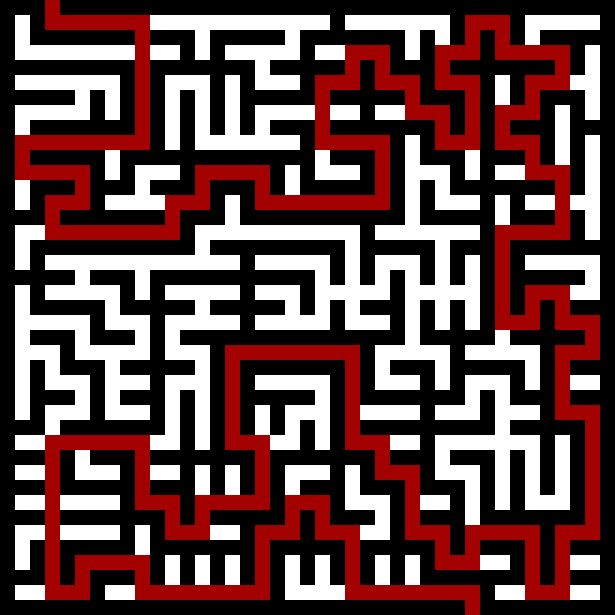
\includegraphics{figurer/middels_lost.png}};
\end{slide}

\begin{slide}
    \node [inner sep=0pt, outer sep=0pt, draw, line width=3mm] at (0, 0) {
\includegraphics[height=700pt]{figurer/vanskelig.png}};
\end{slide}

\begin{slide}
    \node [inner sep=0pt, outer sep=0pt, draw, line width=3mm] at (0, 0) {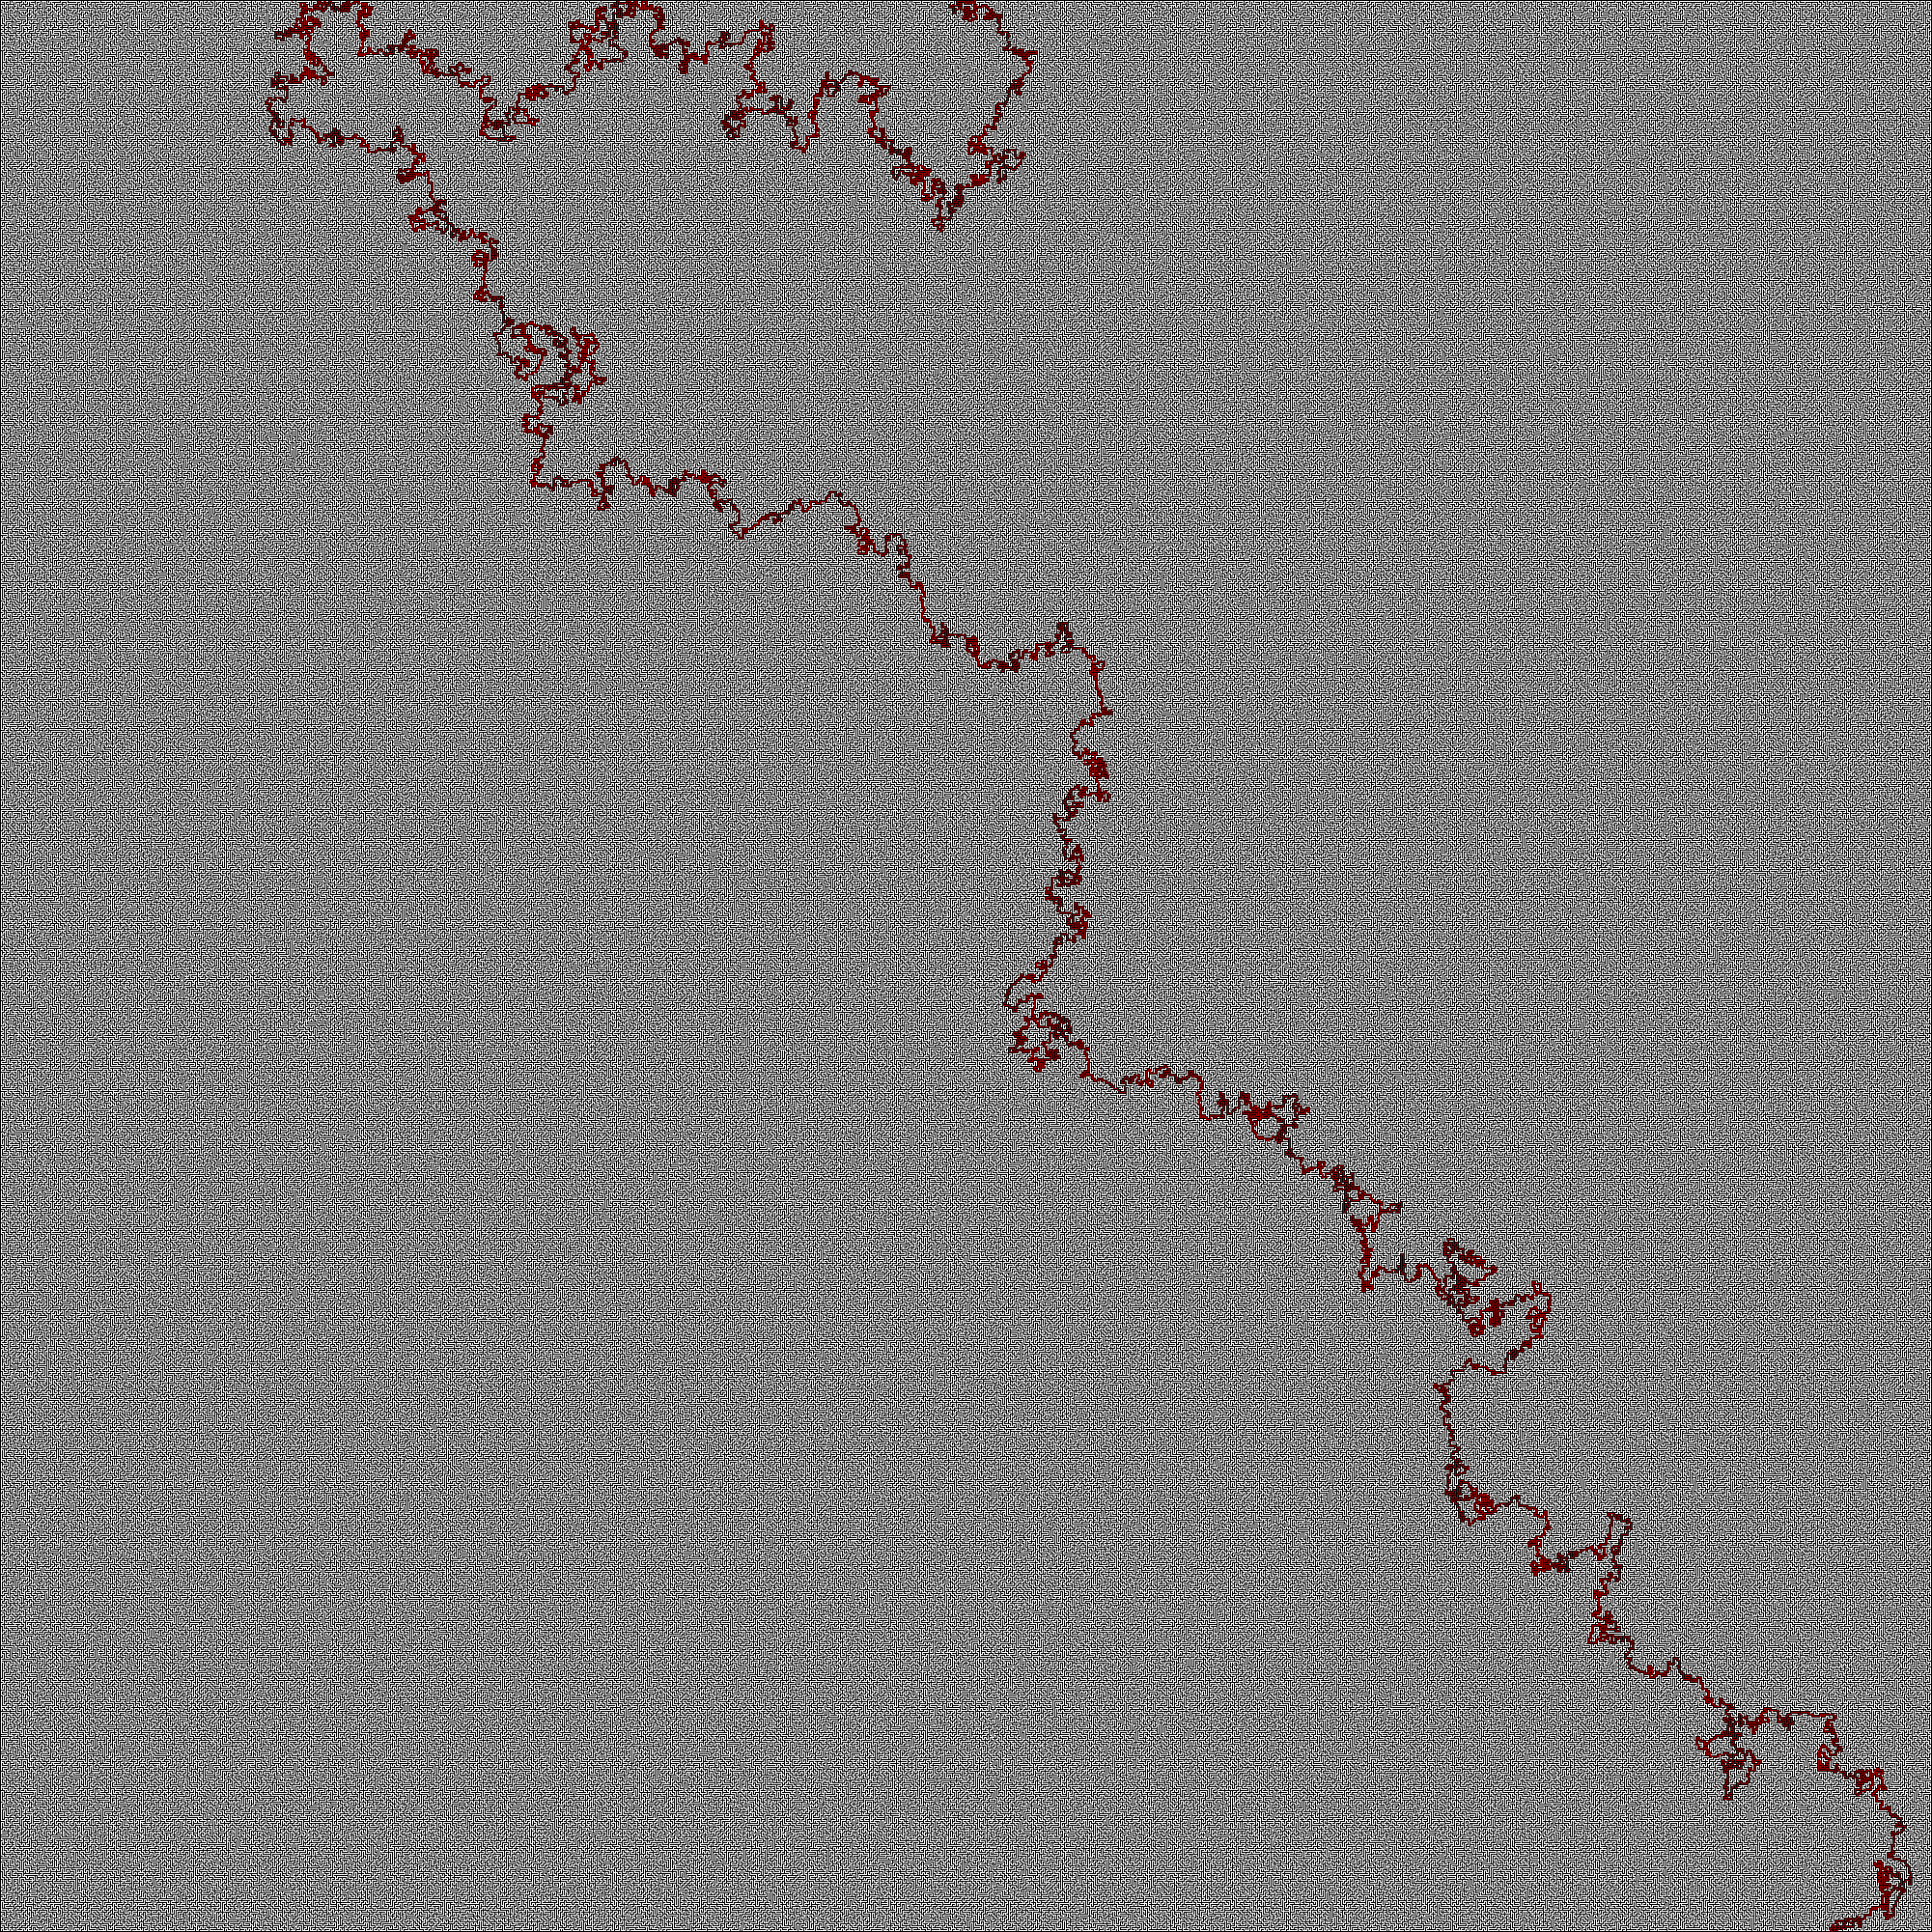
\includegraphics[height=700pt]{figurer/vanskelig_lost.png}};
\end{slide}

\begin{slide}
    \node [align=center, text width=1025pt, scale=2.3, color=highlight, fill=gray] at (0, 0) {\texttt{01011100 01100100 01101111 01100011 01110101 01101101 01100101 01101110 01110100 01100011 01101100 01100001 01110011 01110011 01011011 01100001 00110100 01110000 01100001 01110000 01100101 01110010 01011101 01111011 01100001 01110010 01110100 01101001 01100011 01101100 01100101 01111101 00001010 00001010 01011100 01110101 01110011 01100101 01110000 01100001 01100011 01101011 01100001 01100111 01100101 01111011 01100101 01100001 01101010 01111101 00001010 00001010 01011100 01110100 01101001 01110100 01101100 01100101 01111011 01001101 01100001 01101110 01110101 01110011 00100000 01100110 01101111 01110010 00100000 01110000 01110010 01100101 01110011 01100101 01101110 01110100 01100001 01110011 01101010 01101111 01101110 00100000 01100110 01110010 01100101 01100100 01100001 01100111 00100000 00110010 00111001 00101110 00100000 01101110 01101111 01110110 01100101 01101101 01100010 01100101 01110010 01011100 01011100 01010100 01010000 01000100 00110100 00110001 00110001 00110100 01111101 00001010 01011100 01100001 01110101 01110100 01101000 01101111 01110010 01111011 01000101 01110010 01101001 01101011 00100000 01000001 01101110 01100100 01110010 11101001 00100000 01001010 01100001 01101011 01101111 01100010 01110011 01100101 01101110 01111101 00001010 01011100 01100100 01100001 01110100 01100101 01111011 01111101 00001010 00001010 01011100 01100100 01100101 01100110 01101001 01101110 01100101 01100011 01101111 01101100 01101111 01110010 01111011 01110000 01110010 01101001 01101101 01100001 01110010 01111001 01111101 01111011 01001000 01010100 01001101 01001100 01111101 01111011 01000110 01000110 00111000 00110000 00110000 00110000 01111101 00001010 01011100 01100100 01100101 01100110 01101001 01101110 01100101 01100011 01101111 01101100 01101111 01110010 01111011 01110000 01110010 01101001 01101101 01100001 01110010 01111001 00101101 01100100 01100001 01110010 01101011 01111101 01111011 01001000 01010100 01001101 01001100 01111101 01111011 01000001 00110011 00110000 00110000 00110000 00110000 01111101 00001010 01011100 01100100 01100101 01100110 01101001 01101110 01100101 01100011 01101111 01101100 01101111 01110010 01111011 01110011 01100101 01100011 01101111 01101110 01100100 01100001 01110010 01111001 01111101 01111011 01001000 01010100 01001101 01001100 01111101 01111011 00110000 00110000 01000001 01000110 01000010 00110101 01111101 00001010 01011100 01100100 01100101 01100110 01101001 01101110 01100101 01100011 01101111 01101100 01101111 01110010 01111011 01110011 01100101 01100011 01101111 01101110 01100100 01100001 01110010 01111001 00101101 01100100 01100001 01110010 01101011 01111101 01111011 01001000 01010100 01001101 01001100 01111101 01111011 00110000 00110000 00110100 00110111 00110111 00110111 01111101 00001010 01011100 01100100 01100101 01100110 01101001 01101110 01100101 01100011 01101111 01101100 01101111 01110010 01111011 01101000 01101001 01100111 01101000 01101100 01101001 01100111 01101000 01110100 01111101 01111011 01001000 01010100 01001101 01001100 01111101 01111011 01000101 01000110 01000100 00110010 00111000 01000100 01111101 00001010 00001010 01011100 01101110 01100101 01110111 01100011 01101111 01101101 01101101 01100001 01101110 01100100 01111011 01011100 01101000 01101100 01111101 01011011 00110010 01011101 01011011 01110000 01110010 01101001 01101101 01100001 01110010 01111001 00101101 01100100 01100001 01110010 01101011 01011101 01111011 01011100 01110100 01100101 01111000 01110100 01100011 01101111 01101100 01101111 01110010 01111011 00100011 00110001 01111101 01111011 00100011 00110010 01111101 01111101 00001010 00001010 01011100 01100010 01100101 01100111 01101001 01101110 01111011 01100100 01101111 01100011 01110101 01101101 01100101 01101110 01110100 01111101 00001010 01011100 01101101 01100001 01101011 01100101 01110100 01101001 01110100 01101100 01100101 00001010 00001010 01000100 01100101 01110100 01110100 01100101 00100000 01100101 01110010 00100000 01100101 01101110 00100000 01101100 01100001 01100010 01111001 01110010 01101001 01101110 01110100 00101110 00100000 01010110 01101001 00100000 01110011 01110100 01100001 01110010 01110100 01100101 01110010 00100000 01110000 11100101 00100000 01110100 01101111 01110000 01110000 01100101 01101110 00101100 00100000 01101111 01100111 00100000 01101101 11100101 01101100 01100101 01110100 00100000 01100101 01110010 00100000 11100101 00100000 01100110 01101001 01101110 01101110 01100101 00100000 01110110 01100101 01101001 01100101 01101110 00100000 01110100 01101001 01101100 00100000 01100010 01110101 01101110 01101110 01100101 01101110 00101110 00100000 01000100 01100101 01101110 00100000 01100101 01110010 00100000 01110010 01101001 01101101 01100101 01101100 01101001 01100111 00100000 01101100 01100101 01110100 01110100 00100000 00101101 00101101 00100000 01101101 01100001 01101110 01100111 01100101 00100000 01101000 01100001 01110010 00100000 01101110 01101111 01101011 00100000 01100001 01101100 01101100 01100101 01110010 01100101 01100100 01100101 00100000 01110011 01100101 01110100 01110100 00100000 01011100 01101000 01101100 01111011 01101100 11111000 01110011 01101110 01101001 01101110 01100111 01100101 01101110 01111101 00101110 00001010 00001010 01001100 01100001 01100010 01111001 01110010 01101001 01101110 01110100 01100101 01110010 00100000 01101011 01100001 01101110 00100000 01110011 01100101 01101100 01110110 01100110 11111000 01101100 01100111 01100101 01101100 01101001 01100111 00100000 01110110 11100110 01110010 01100101 00100000 01110110 01100001 01101110 01110011 01101011 01100101 01101100 01101001 01100111 01100101 01110010 01100101 00101110 00100000 01011100 01101000 01101100 01111011 01000100 01100101 01101110 01101110 01100101 01111101 00100000 01100101 01110010 00100000 01110011 01110100 11111000 01110010 01110010 01100101 00101100 00100000 01101111 01100111 00100000 01100100 01100101 01110100 00100000 01101000 01100001 01100100 01100100 01100101 00100000 01110100 01100001 01110100 01110100 00100000 01100101 01101110 00100000 01110011 01110100 01110101 01101110 01100100 00100000 11100101 00100000 01100110 01101001 01101110 01101110 01100101 00100000 01100001 01110100 00100000 01011100 01101000 01101100 01111011 01100100 01100101 01110100 01110100 01100101 01111101 00100000 01100101 01110010 00100000 01101100 11111000 01110011 01101110 01101001 01101110 01100111 01100101 01101110 00101110 00001010 00001010 01011100 01101000 01101100 01111011 01000100 01100101 01101110 01101110 01100101 01111101 00100000 01101100 01100001 01100010 01111001 01110010 01101001 01101110 01110100 01100101 01101110 00100000 01100101 01110010 00100000 01110011 11100101 00100000 01110011 01110100 01101111 01110010 00100000 01100001 01110100 00100000 01110110 01101001 00100000 01101001 01101011 01101011 01100101 00100000 01100101 01101110 01100111 01100001 01101110 01100111 00100000 01100111 01110010 01100101 01101001 01100101 01110010 00100000 11100101 00100000 01110011 01100101 00100000 01100001 01110100 00100000 01100100 01100101 01110100 00100000 01011100 01100101 01101101 01110000 01101000 01111011 01100101 01110010 01111101 00100000 01100101 01101110 00101110 00100000 11000101 00100000 01100110 01101001 01101110 01101110 01100101 00100000 01011100 01101000 01101100 01111011 01101100 11111000 01110011 01101110 01101001 01101110 01100111 01100101 01101110 01111101 00100000 01101000 01100001 01100100 01100100 01100101 00100000 01110100 01100001 01110100 01110100 00100000 01100110 01101100 01100101 01110010 01100101 00100000 01100100 01100001 01100111 01100101 01110010 00101100 00100000 01101111 01101101 00100000 01101101 01100001 01101110 00100000 01101001 00100000 01100100 01100101 01110100 00100000 01101000 01100101 01101100 01100101 00100000 01110100 01100001 01110100 01110100 00100000 01101000 01100001 01100100 01100100 01100101 00100000 01100110 11100101 01110100 01110100 00100000 01100100 01100101 01110100 00100000 01110100 01101001 01101100 00101110 00100000 01001110 01101111 01100101 01101110 00100000 01100111 01100001 01101110 01100111 01100101 01110010 00100000 01100101 01110010 00100000 01110110 01101001 00100000 01100100 01100101 01110010 01101001 01101101 01101111 01110100 00100000 01101110 11111000 01100100 01110100 00100000 01110100 01101001 01101100 00100000 11100101 00100000 01101100 11111000 01110011 01100101 00100000 01101100 01100001 01100010 01111001 01110010 01101001 01101110 01110100 01100101 01110010 00100000 01100001 01110110 00100000 01100100 01100101 01101110 01101110 01100101 00100000 01110011 01110100 11111000 01110010 01110010 01100101 01101100 01110011 01100101 01101110 00101100 00100000 01101111 01100111 00100000 01100100 01100001 00100000 01100010 01110010 01110101 01101011 01100101 01110010 00100000 01110110 01101001 00100000 01100100 01100001 01110100 01100001 01101101 01100001 01110011 01101011 01101001 01101110 01100101 01110010 00101110 00001010 00001010 01011100 01100101 01101110 01100100 01111011 01100100 01101111 01100011 01110101 01101101 01100101 01101110 01110100 01111101}};
\end{slide}

\begin{slide}
    \node (enkel) [draw, line width=3mm, inner sep=0pt] at (0, 0) {
\includegraphics{figurer/enkel.png}};
\end{slide}

\begin{slide}
    \coordinate (A) at (-9, -9);
    \coordinate (B) at (9, 9);
    \node [draw, line width=3mm, inner sep=0pt] at (0, 0) {
\includegraphics{figurer/enkel.png}};
    \begin{scope}[scale=.98]
        \draw [line width=2.9mm, color=orange] (-9, -9) rectangle (9, 9);
        \foreach \x in {-9, -7.2, -5.4, ..., 9.1} { 
            \draw[orange, line width=2mm] (\x, -9) -- (\x, 9);
            \draw[orange, line width=2mm] (-9, \x) -- (9, \x); 
        }
    \end{scope}
\end{slide}

\begin{slide}
    \tikzset{data/.style={color=orange, line width=2mm}}
    \coordinate (A) at (-9, -9);
    \coordinate (B) at (9, 9);
    \node [draw, line width=3mm, inner sep=0pt] at (0, 0) {
\includegraphics{figurer/enkel.png}};

    \begin{scope}[scale=.98]
        \draw [line width=2.9mm, color=orange] (-9, -9) rectangle (9, 9);
        % Vertical walls
        \foreach \x in {-9, 7.2} {
            \foreach \y in {-9, -7.2, ..., 9} {
                \draw[color=orange, line width=2mm] (\x, \y) rectangle node[pos=0.5, scale=3] {\texttt{0}} ++(1.8, 1.8);
            }
        }
        % Bottom line
        \foreach \x in {-7.2, -5.4, -3.6, -1.8, 0, 1.8, 5.4} {
            \draw[data] (\x, -9) rectangle node[pos=0.5, scale=3] {\texttt{0}} ++(1.8, 1.8);
        }
        \draw[data] (3.6, -9) rectangle node[pos=0.5, scale=3] {\texttt{1}} ++(1.8, 1.8);
    
        % Second line
        \foreach \x in {-7.2, -5.4, ..., 5.5} {
            \draw[data] (\x, -7.2) rectangle node[pos=0.5, scale=3] {\texttt{1}} ++(1.8, 1.8);
        }
    
        % Third line
        % Walls
        \foreach \x in {-5.4, -1.8, 1.8, 3.6} {
            \draw[data] (\x, -5.4) rectangle node[pos=0.5, scale=3] {\texttt{0}} ++(1.8, 1.8);
        }
        % Floor
        \foreach \x in {-7.2, -3.6, 0, 5.4} {
            \draw[data] (\x, -5.4) rectangle node[pos=0.5, scale=3] {\texttt{1}} ++(1.8, 1.8);
        }
    
        % Fourth line
        % Walls
        \foreach \x in {-7.2, -5.4, -3.6, -1.8, 1.8, 3.6, 5.4} {
            \draw[data] (\x, -3.6) rectangle node[pos=0.5, scale=3] {\texttt{0}} ++(1.8, 1.8);
        }
        % Floor
        \foreach \x in {0} {
            \draw[data] (\x, -3.6) rectangle node[pos=0.5, scale=3] {\texttt{1}} ++(1.8, 1.8);
        }
    
        % Fifth line
        % Walls
        \foreach \x in {1.8} {
            \draw[data] (\x, -1.8) rectangle node[pos=0.5, scale=3] {\texttt{0}} ++(1.8, 1.8);
        }
        % Floor
        \foreach \x in {-7.2, -5.4, ..., 0.1, 3.6, 5.4} {
            \draw[data] (\x, -1.8) rectangle node[pos=0.5, scale=3] {\texttt{1}} ++(1.8, 1.8);
        }
    
        % Sixth line
        % Walls
        \foreach \x in {-5.4, -1.8, 1.8, 3.6} {
            \draw[data] (\x, 0) rectangle node[pos=0.5, scale=3] {\texttt{0}} ++(1.8, 1.8);
        }
        % Floor
        \foreach \x in {-7.2, -3.6, 0, 5.4} {
            \draw[data] (\x, 0) rectangle node[pos=0.5, scale=3] {\texttt{1}} ++(1.8, 1.8);
        }
    
        % Seventh line
        % Walls
        \foreach \x in {-1.8, 3.6} {
            \draw[data] (\x, 1.8) rectangle node[pos=0.5, scale=3] {\texttt{0}} ++(1.8, 1.8);
        }
        % Floor
        \foreach \x in {-7.2, -5.4, -3.6, 0, 1.8, 5.4} {
            \draw[data] (\x, 1.8) rectangle node[pos=0.5, scale=3] {\texttt{1}} ++(1.8, 1.8);
        }
    
        % Seventh line
        % Walls
        \foreach \x in {-5.4, -3.6, -1.8, 0, 3.6} {
            \draw[data] (\x, 3.6) rectangle node[pos=0.5, scale=3] {\texttt{0}} ++(1.8, 1.8);
        }
        % Floor
        \foreach \x in {-7.2, 1.8, 5.4} {
            \draw[data] (\x, 3.6) rectangle node[pos=0.5, scale=3] {\texttt{1}} ++(1.8, 1.8);
        }
    
        % Eight line
        % Floor
        \foreach \x in {-7.2, -5.4, ..., 5.5} {
            \draw[data] (\x, 5.4) rectangle node[pos=0.5, scale=3] {\texttt{1}} ++(1.8, 1.8);
        }
    
        % Top line
        % Walls
        \foreach \x in {-7.2, -5.4, -1.8, 0, 1.8, 3.6, 5.4} {
            \draw[data] (\x, 7.2) rectangle node[pos=0.5, scale=3] {\texttt{0}} ++(1.8, 1.8);
        }
        % Floor
        \foreach \x in {-3.6} {
            \draw[data] (\x, 7.2) rectangle node[pos=0.5, scale=3] {\texttt{1}} ++(1.8, 1.8);
        }
    \end{scope}
\end{slide}

\begin{slide}
    \tikzset{data/.style={color=black, line width=2mm}}
    \begin{scope}[scale=.98]
        \draw [line width=2.9mm, color=black] (-9, -9) rectangle (9, 9);
        % Vertical walls
        \foreach \x in {-9, 7.2} {
            \foreach \y in {-9, -7.2, ..., 9} {
                \draw[data] (\x, \y) rectangle node[pos=0.5, scale=3] {\texttt{0}} ++(1.8, 1.8);
            }
        }
        % Bottom line
        \foreach \x in {-7.2, -5.4, -3.6, -1.8, 0, 1.8, 5.4} {
            \draw[data] (\x, -9) rectangle node[pos=0.5, scale=3] {\texttt{0}} ++(1.8, 1.8);
        }
        \draw[data] (3.6, -9) rectangle node[pos=0.5, scale=3] {\texttt{1}} ++(1.8, 1.8);
    
        % Second line
        \foreach \x in {-7.2, -5.4, ..., 5.5} {
            \draw[data] (\x, -7.2) rectangle node[pos=0.5, scale=3] {\texttt{1}} ++(1.8, 1.8);
        }
    
        % Third line
        % Walls
        \foreach \x in {-5.4, -1.8, 1.8, 3.6} {
            \draw[data] (\x, -5.4) rectangle node[pos=0.5, scale=3] {\texttt{0}} ++(1.8, 1.8);
        }
        % Floor
        \foreach \x in {-7.2, -3.6, 0, 5.4} {
            \draw[data] (\x, -5.4) rectangle node[pos=0.5, scale=3] {\texttt{1}} ++(1.8, 1.8);
        }
    
        % Fourth line
        % Walls
        \foreach \x in {-7.2, -5.4, -3.6, -1.8, 1.8, 3.6, 5.4} {
            \draw[data] (\x, -3.6) rectangle node[pos=0.5, scale=3] {\texttt{0}} ++(1.8, 1.8);
        }
        % Floor
        \foreach \x in {0} {
            \draw[data] (\x, -3.6) rectangle node[pos=0.5, scale=3] {\texttt{1}} ++(1.8, 1.8);
        }
    
        % Fifth line
        % Walls
        \foreach \x in {1.8} {
            \draw[data] (\x, -1.8) rectangle node[pos=0.5, scale=3] {\texttt{0}} ++(1.8, 1.8);
        }
        % Floor
        \foreach \x in {-7.2, -5.4, ..., 0.1, 3.6, 5.4} {
            \draw[data] (\x, -1.8) rectangle node[pos=0.5, scale=3] {\texttt{1}} ++(1.8, 1.8);
        }
    
        % Sixth line
        % Walls
        \foreach \x in {-5.4, -1.8, 1.8, 3.6} {
            \draw[data] (\x, 0) rectangle node[pos=0.5, scale=3] {\texttt{0}} ++(1.8, 1.8);
        }
        % Floor
        \foreach \x in {-7.2, -3.6, 0, 5.4} {
            \draw[data] (\x, 0) rectangle node[pos=0.5, scale=3] {\texttt{1}} ++(1.8, 1.8);
        }
    
        % Seventh line
        % Walls
        \foreach \x in {-1.8, 3.6} {
            \draw[data] (\x, 1.8) rectangle node[pos=0.5, scale=3] {\texttt{0}} ++(1.8, 1.8);
        }
        % Floor
        \foreach \x in {-7.2, -5.4, -3.6, 0, 1.8, 5.4} {
            \draw[data] (\x, 1.8) rectangle node[pos=0.5, scale=3] {\texttt{1}} ++(1.8, 1.8);
        }
    
        % Seventh line
        % Walls
        \foreach \x in {-5.4, -3.6, -1.8, 0, 3.6} {
            \draw[data] (\x, 3.6) rectangle node[pos=0.5, scale=3] {\texttt{0}} ++(1.8, 1.8);
        }
        % Floor
        \foreach \x in {-7.2, 1.8, 5.4} {
            \draw[data] (\x, 3.6) rectangle node[pos=0.5, scale=3] {\texttt{1}} ++(1.8, 1.8);
        }
    
        % Eight line
        % Floor
        \foreach \x in {-7.2, -5.4, ..., 5.5} {
            \draw[data] (\x, 5.4) rectangle node[pos=0.5, scale=3] {\texttt{1}} ++(1.8, 1.8);
        }
    
        % Top line
        % Walls
        \foreach \x in {-7.2, -5.4, -1.8, 0, 1.8, 3.6, 5.4} {
            \draw[data] (\x, 7.2) rectangle node[pos=0.5, scale=3] {\texttt{0}} ++(1.8, 1.8);
        }
        % Floor
        \foreach \x in {-3.6} {
            \draw[data] (\x, 7.2) rectangle node[pos=0.5, scale=3] {\texttt{1}} ++(1.8, 1.8);
        }
    \end{scope}
\end{slide}

\begin{slide}
    \tikzset{data/.style={color=black, line width=2mm}}

    \node [opacity=0.3] at (0, 0) {
\includegraphics{figurer/enkel.png}};

    \begin{scope}[scale=.98]
        \draw [line width=2.9mm, color=black] (-9, -9) rectangle (9, 9);
        % Vertical walls
        \foreach \x in {-9, 7.2} {
            \foreach \y in {-9, -7.2, ..., 9} {
                \draw[data] (\x, \y) rectangle node[pos=0.5, scale=3] {\texttt{0}} ++(1.8, 1.8);
            }
        }
        % Bottom line
        \foreach \x in {-7.2, -5.4, -3.6, -1.8, 0, 1.8, 5.4} {
            \draw[data] (\x, -9) rectangle node[pos=0.5, scale=3] {\texttt{0}} ++(1.8, 1.8);
        }
        \draw[data] (3.6, -9) rectangle node[pos=0.5, scale=3] {\texttt{1}} ++(1.8, 1.8);
    
        % Second line
        \foreach \x in {-7.2, -5.4, ..., 5.5} {
            \draw[data] (\x, -7.2) rectangle node[pos=0.5, scale=3] {\texttt{1}} ++(1.8, 1.8);
        }
    
        % Third line
        % Walls
        \foreach \x in {-5.4, -1.8, 1.8, 3.6} {
            \draw[data] (\x, -5.4) rectangle node[pos=0.5, scale=3] {\texttt{0}} ++(1.8, 1.8);
        }
        % Floor
        \foreach \x in {-7.2, -3.6, 0, 5.4} {
            \draw[data] (\x, -5.4) rectangle node[pos=0.5, scale=3] {\texttt{1}} ++(1.8, 1.8);
        }
    
        % Fourth line
        % Walls
        \foreach \x in {-7.2, -5.4, -3.6, -1.8, 1.8, 3.6, 5.4} {
            \draw[data] (\x, -3.6) rectangle node[pos=0.5, scale=3] {\texttt{0}} ++(1.8, 1.8);
        }
        % Floor
        \foreach \x in {0} {
            \draw[data] (\x, -3.6) rectangle node[pos=0.5, scale=3] {\texttt{1}} ++(1.8, 1.8);
        }
    
        % Fifth line
        % Walls
        \foreach \x in {1.8} {
            \draw[data] (\x, -1.8) rectangle node[pos=0.5, scale=3] {\texttt{0}} ++(1.8, 1.8);
        }
        % Floor
        \foreach \x in {-7.2, -5.4, ..., 0.1, 3.6, 5.4} {
            \draw[data] (\x, -1.8) rectangle node[pos=0.5, scale=3] {\texttt{1}} ++(1.8, 1.8);
        }
    
        % Sixth line
        % Walls
        \foreach \x in {-5.4, -1.8, 1.8, 3.6} {
            \draw[data] (\x, 0) rectangle node[pos=0.5, scale=3] {\texttt{0}} ++(1.8, 1.8);
        }
        % Floor
        \foreach \x in {-7.2, -3.6, 0, 5.4} {
            \draw[data] (\x, 0) rectangle node[pos=0.5, scale=3] {\texttt{1}} ++(1.8, 1.8);
        }
    
        % Seventh line
        % Walls
        \foreach \x in {-1.8, 3.6} {
            \draw[data] (\x, 1.8) rectangle node[pos=0.5, scale=3] {\texttt{0}} ++(1.8, 1.8);
        }
        % Floor
        \foreach \x in {-7.2, -5.4, -3.6, 0, 1.8, 5.4} {
            \draw[data] (\x, 1.8) rectangle node[pos=0.5, scale=3] {\texttt{1}} ++(1.8, 1.8);
        }
    
        % Seventh line
        % Walls
        \foreach \x in {-5.4, -3.6, -1.8, 0, 3.6} {
            \draw[data] (\x, 3.6) rectangle node[pos=0.5, scale=3] {\texttt{0}} ++(1.8, 1.8);
        }
        % Floor
        \foreach \x in {-7.2, 1.8, 5.4} {
            \draw[data] (\x, 3.6) rectangle node[pos=0.5, scale=3] {\texttt{1}} ++(1.8, 1.8);
        }
    
        % Eight line
        % Floor
        \foreach \x in {-7.2, -5.4, ..., 5.5} {
            \draw[data] (\x, 5.4) rectangle node[pos=0.5, scale=3] {\texttt{1}} ++(1.8, 1.8);
        }
    
        % Top line
        % Walls
        \foreach \x in {-7.2, -5.4, -1.8, 0, 1.8, 3.6, 5.4} {
            \draw[data] (\x, 7.2) rectangle node[pos=0.5, scale=3] {\texttt{0}} ++(1.8, 1.8);
        }
        % Floor
        \foreach \x in {-3.6} {
            \draw[data] (\x, 7.2) rectangle node[pos=0.5, scale=3] {\texttt{1}} ++(1.8, 1.8);
        }
    \end{scope}
\end{slide}

\begin{slide}
    \tikzset{data/.style={color=black, line width=2mm}}
    \node [opacity=0.3] at (0, 0) {
\includegraphics{figurer/enkel.png}};

    \begin{scope}[scale=.98]
        \fill[color=orange] (-3.6, 7.2) rectangle ++(1.8, 1.8);

        \draw [line width=2.9mm, color=black] (-9, -9) rectangle (9, 9);
        % Vertical walls
        \foreach \x in {-9, 7.2} {
            \foreach \y in {-9, -7.2, ..., 9} {
                \draw[data] (\x, \y) rectangle node[pos=0.5, scale=3] {\texttt{0}} ++(1.8, 1.8);
            }
        }
        % Bottom line
        \foreach \x in {-7.2, -5.4, -3.6, -1.8, 0, 1.8, 5.4} {
            \draw[data] (\x, -9) rectangle node[pos=0.5, scale=3] {\texttt{0}} ++(1.8, 1.8);
        }
        \draw[data] (3.6, -9) rectangle node[pos=0.5, scale=3] {\texttt{1}} ++(1.8, 1.8);
    
        % Second line
        \foreach \x in {-7.2, -5.4, ..., 5.5} {
            \draw[data] (\x, -7.2) rectangle node[pos=0.5, scale=3] {\texttt{1}} ++(1.8, 1.8);
        }
    
        % Third line
        % Walls
        \foreach \x in {-5.4, -1.8, 1.8, 3.6} {
            \draw[data] (\x, -5.4) rectangle node[pos=0.5, scale=3] {\texttt{0}} ++(1.8, 1.8);
        }
        % Floor
        \foreach \x in {-7.2, -3.6, 0, 5.4} {
            \draw[data] (\x, -5.4) rectangle node[pos=0.5, scale=3] {\texttt{1}} ++(1.8, 1.8);
        }
    
        % Fourth line
        % Walls
        \foreach \x in {-7.2, -5.4, -3.6, -1.8, 1.8, 3.6, 5.4} {
            \draw[data] (\x, -3.6) rectangle node[pos=0.5, scale=3] {\texttt{0}} ++(1.8, 1.8);
        }
        % Floor
        \foreach \x in {0} {
            \draw[data] (\x, -3.6) rectangle node[pos=0.5, scale=3] {\texttt{1}} ++(1.8, 1.8);
        }
    
        % Fifth line
        % Walls
        \foreach \x in {1.8} {
            \draw[data] (\x, -1.8) rectangle node[pos=0.5, scale=3] {\texttt{0}} ++(1.8, 1.8);
        }
        % Floor
        \foreach \x in {-7.2, -5.4, ..., 0.1, 3.6, 5.4} {
            \draw[data] (\x, -1.8) rectangle node[pos=0.5, scale=3] {\texttt{1}} ++(1.8, 1.8);
        }
    
        % Sixth line
        % Walls
        \foreach \x in {-5.4, -1.8, 1.8, 3.6} {
            \draw[data] (\x, 0) rectangle node[pos=0.5, scale=3] {\texttt{0}} ++(1.8, 1.8);
        }
        % Floor
        \foreach \x in {-7.2, -3.6, 0, 5.4} {
            \draw[data] (\x, 0) rectangle node[pos=0.5, scale=3] {\texttt{1}} ++(1.8, 1.8);
        }
    
        % Seventh line
        % Walls
        \foreach \x in {-1.8, 3.6} {
            \draw[data] (\x, 1.8) rectangle node[pos=0.5, scale=3] {\texttt{0}} ++(1.8, 1.8);
        }
        % Floor
        \foreach \x in {-7.2, -5.4, -3.6, 0, 1.8, 5.4} {
            \draw[data] (\x, 1.8) rectangle node[pos=0.5, scale=3] {\texttt{1}} ++(1.8, 1.8);
        }
    
        % Seventh line
        % Walls
        \foreach \x in {-5.4, -3.6, -1.8, 0, 3.6} {
            \draw[data] (\x, 3.6) rectangle node[pos=0.5, scale=3] {\texttt{0}} ++(1.8, 1.8);
        }
        % Floor
        \foreach \x in {-7.2, 1.8, 5.4} {
            \draw[data] (\x, 3.6) rectangle node[pos=0.5, scale=3] {\texttt{1}} ++(1.8, 1.8);
        }
    
        % Eight line
        % Floor
        \foreach \x in {-7.2, -5.4, ..., 5.5} {
            \draw[data] (\x, 5.4) rectangle node[pos=0.5, scale=3] {\texttt{1}} ++(1.8, 1.8);
        }
    
        % Top line
        % Walls
        \foreach \x in {-7.2, -5.4, -1.8, 0, 1.8, 3.6, 5.4} {
            \draw[data] (\x, 7.2) rectangle node[pos=0.5, scale=3] {\texttt{0}} ++(1.8, 1.8);
        }
        % Floor
        \foreach \x in {-3.6} {
            \draw[data] (\x, 7.2) rectangle node[pos=0.5, scale=3] {\texttt{1}} ++(1.8, 1.8);
        }
    \end{scope}
\end{slide}

\begin{slide}
    \tikzset{data/.style={color=black, line width=2mm}}
    \node [opacity=0.3] at (0, 0) {
\includegraphics{figurer/enkel.png}};

    \begin{scope}[scale=.98]
        \fill[color=orange] (-3.6, 7.2) rectangle ++(1.8, 1.8);
        \fill[color=orange] (3.6, -9) rectangle ++(1.8, 1.8);

        \draw [line width=2.9mm, color=black] (-9, -9) rectangle (9, 9);
        % Vertical walls
        \foreach \x in {-9, 7.2} {
            \foreach \y in {-9, -7.2, ..., 9} {
                \draw[data] (\x, \y) rectangle node[pos=0.5, scale=3] {\texttt{0}} ++(1.8, 1.8);
            }
        }
        % Bottom line
        \foreach \x in {-7.2, -5.4, -3.6, -1.8, 0, 1.8, 5.4} {
            \draw[data] (\x, -9) rectangle node[pos=0.5, scale=3] {\texttt{0}} ++(1.8, 1.8);
        }
        \draw[data] (3.6, -9) rectangle node[pos=0.5, scale=3] {\texttt{1}} ++(1.8, 1.8);
    
        % Second line
        \foreach \x in {-7.2, -5.4, ..., 5.5} {
            \draw[data] (\x, -7.2) rectangle node[pos=0.5, scale=3] {\texttt{1}} ++(1.8, 1.8);
        }
    
        % Third line
        % Walls
        \foreach \x in {-5.4, -1.8, 1.8, 3.6} {
            \draw[data] (\x, -5.4) rectangle node[pos=0.5, scale=3] {\texttt{0}} ++(1.8, 1.8);
        }
        % Floor
        \foreach \x in {-7.2, -3.6, 0, 5.4} {
            \draw[data] (\x, -5.4) rectangle node[pos=0.5, scale=3] {\texttt{1}} ++(1.8, 1.8);
        }
    
        % Fourth line
        % Walls
        \foreach \x in {-7.2, -5.4, -3.6, -1.8, 1.8, 3.6, 5.4} {
            \draw[data] (\x, -3.6) rectangle node[pos=0.5, scale=3] {\texttt{0}} ++(1.8, 1.8);
        }
        % Floor
        \foreach \x in {0} {
            \draw[data] (\x, -3.6) rectangle node[pos=0.5, scale=3] {\texttt{1}} ++(1.8, 1.8);
        }
    
        % Fifth line
        % Walls
        \foreach \x in {1.8} {
            \draw[data] (\x, -1.8) rectangle node[pos=0.5, scale=3] {\texttt{0}} ++(1.8, 1.8);
        }
        % Floor
        \foreach \x in {-7.2, -5.4, ..., 0.1, 3.6, 5.4} {
            \draw[data] (\x, -1.8) rectangle node[pos=0.5, scale=3] {\texttt{1}} ++(1.8, 1.8);
        }
    
        % Sixth line
        % Walls
        \foreach \x in {-5.4, -1.8, 1.8, 3.6} {
            \draw[data] (\x, 0) rectangle node[pos=0.5, scale=3] {\texttt{0}} ++(1.8, 1.8);
        }
        % Floor
        \foreach \x in {-7.2, -3.6, 0, 5.4} {
            \draw[data] (\x, 0) rectangle node[pos=0.5, scale=3] {\texttt{1}} ++(1.8, 1.8);
        }
    
        % Seventh line
        % Walls
        \foreach \x in {-1.8, 3.6} {
            \draw[data] (\x, 1.8) rectangle node[pos=0.5, scale=3] {\texttt{0}} ++(1.8, 1.8);
        }
        % Floor
        \foreach \x in {-7.2, -5.4, -3.6, 0, 1.8, 5.4} {
            \draw[data] (\x, 1.8) rectangle node[pos=0.5, scale=3] {\texttt{1}} ++(1.8, 1.8);
        }
    
        % Seventh line
        % Walls
        \foreach \x in {-5.4, -3.6, -1.8, 0, 3.6} {
            \draw[data] (\x, 3.6) rectangle node[pos=0.5, scale=3] {\texttt{0}} ++(1.8, 1.8);
        }
        % Floor
        \foreach \x in {-7.2, 1.8, 5.4} {
            \draw[data] (\x, 3.6) rectangle node[pos=0.5, scale=3] {\texttt{1}} ++(1.8, 1.8);
        }
    
        % Eight line
        % Floor
        \foreach \x in {-7.2, -5.4, ..., 5.5} {
            \draw[data] (\x, 5.4) rectangle node[pos=0.5, scale=3] {\texttt{1}} ++(1.8, 1.8);
        }
    
        % Top line
        % Walls
        \foreach \x in {-7.2, -5.4, -1.8, 0, 1.8, 3.6, 5.4} {
            \draw[data] (\x, 7.2) rectangle node[pos=0.5, scale=3] {\texttt{0}} ++(1.8, 1.8);
        }
        % Floor
        \foreach \x in {-3.6} {
            \draw[data] (\x, 7.2) rectangle node[pos=0.5, scale=3] {\texttt{1}} ++(1.8, 1.8);
        }
    \end{scope}
\end{slide}

\begin{slide}
    \tikzset{data/.style={color=black, line width=2mm}}
    \node [opacity=0.3] at (0, 0) {
\includegraphics{figurer/enkel.png}};

    \begin{scope}[scale=.98]
        \fill[color=orange] (-3.6, 7.2) rectangle ++(1.8, 1.8);
        \fill[color=orange] (3.6, -9) rectangle ++(1.8, 1.8);
        
        \fill[color=secondary] (-3.6, 5.4) rectangle ++(1.8, 1.8);

        \begin{scope}
                \draw [line width=2.9mm, color=black] (-9, -9) rectangle (9, 9);
                % Vertical walls
                \foreach \x in {-9, 7.2} {
                    \foreach \y in {-9, -7.2, ..., 9} {
                        \draw[data] (\x, \y) rectangle node[pos=0.5, scale=3] {\texttt{0}} ++(1.8, 1.8);
                    }
                }
                % Bottom line
                \foreach \x in {-7.2, -5.4, -3.6, -1.8, 0, 1.8, 5.4} {
                    \draw[data] (\x, -9) rectangle node[pos=0.5, scale=3] {\texttt{0}} ++(1.8, 1.8);
                }
                \draw[data] (3.6, -9) rectangle node[pos=0.5, scale=3] {\texttt{1}} ++(1.8, 1.8);
            
                % Second line
                \foreach \x in {-7.2, -5.4, ..., 5.5} {
                    \draw[data] (\x, -7.2) rectangle node[pos=0.5, scale=3] {\texttt{1}} ++(1.8, 1.8);
                }
            
                % Third line
                % Walls
                \foreach \x in {-5.4, -1.8, 1.8, 3.6} {
                    \draw[data] (\x, -5.4) rectangle node[pos=0.5, scale=3] {\texttt{0}} ++(1.8, 1.8);
                }
                % Floor
                \foreach \x in {-7.2, -3.6, 0, 5.4} {
                    \draw[data] (\x, -5.4) rectangle node[pos=0.5, scale=3] {\texttt{1}} ++(1.8, 1.8);
                }
            
                % Fourth line
                % Walls
                \foreach \x in {-7.2, -5.4, -3.6, -1.8, 1.8, 3.6, 5.4} {
                    \draw[data] (\x, -3.6) rectangle node[pos=0.5, scale=3] {\texttt{0}} ++(1.8, 1.8);
                }
                % Floor
                \foreach \x in {0} {
                    \draw[data] (\x, -3.6) rectangle node[pos=0.5, scale=3] {\texttt{1}} ++(1.8, 1.8);
                }
            
                % Fifth line
                % Walls
                \foreach \x in {1.8} {
                    \draw[data] (\x, -1.8) rectangle node[pos=0.5, scale=3] {\texttt{0}} ++(1.8, 1.8);
                }
                % Floor
                \foreach \x in {-7.2, -5.4, ..., 0.1, 3.6, 5.4} {
                    \draw[data] (\x, -1.8) rectangle node[pos=0.5, scale=3] {\texttt{1}} ++(1.8, 1.8);
                }
            
                % Sixth line
                % Walls
                \foreach \x in {-5.4, -1.8, 1.8, 3.6} {
                    \draw[data] (\x, 0) rectangle node[pos=0.5, scale=3] {\texttt{0}} ++(1.8, 1.8);
                }
                % Floor
                \foreach \x in {-7.2, -3.6, 0, 5.4} {
                    \draw[data] (\x, 0) rectangle node[pos=0.5, scale=3] {\texttt{1}} ++(1.8, 1.8);
                }
            
                % Seventh line
                % Walls
                \foreach \x in {-1.8, 3.6} {
                    \draw[data] (\x, 1.8) rectangle node[pos=0.5, scale=3] {\texttt{0}} ++(1.8, 1.8);
                }
                % Floor
                \foreach \x in {-7.2, -5.4, -3.6, 0, 1.8, 5.4} {
                    \draw[data] (\x, 1.8) rectangle node[pos=0.5, scale=3] {\texttt{1}} ++(1.8, 1.8);
                }
            
                % Seventh line
                % Walls
                \foreach \x in {-5.4, -3.6, -1.8, 0, 3.6} {
                    \draw[data] (\x, 3.6) rectangle node[pos=0.5, scale=3] {\texttt{0}} ++(1.8, 1.8);
                }
                % Floor
                \foreach \x in {-7.2, 1.8, 5.4} {
                    \draw[data] (\x, 3.6) rectangle node[pos=0.5, scale=3] {\texttt{1}} ++(1.8, 1.8);
                }
            
                % Eight line
                % Floor
                \foreach \x in {-7.2, -5.4, ..., 5.5} {
                    \draw[data] (\x, 5.4) rectangle node[pos=0.5, scale=3] {\texttt{1}} ++(1.8, 1.8);
                }
            
                % Top line
                % Walls
                \foreach \x in {-7.2, -5.4, -1.8, 0, 1.8, 3.6, 5.4} {
                    \draw[data] (\x, 7.2) rectangle node[pos=0.5, scale=3] {\texttt{0}} ++(1.8, 1.8);
                }
                % Floor
                \foreach \x in {-3.6} {
                    \draw[data] (\x, 7.2) rectangle node[pos=0.5, scale=3] {\texttt{1}} ++(1.8, 1.8);
                }
            \end{scope}
        \end{scope}
\end{slide}

\begin{slide}
    \tikzset{data/.style={color=black, line width=2mm}}
    \node [opacity=0.3] at (0, 0) {
\includegraphics{figurer/enkel.png}};

    \begin{scope}[scale=.98]
        \fill[color=orange] (-3.6, 7.2) rectangle ++(1.8, 1.8);
        \fill[color=orange] (3.6, -9) rectangle ++(1.8, 1.8);
        
        \fill[color=secondary] (-5.4, 5.4) rectangle ++(1.8, 1.8);
        \fill[color=secondary] (-3.6, 5.4) rectangle ++(1.8, 1.8);

        \begin{scope}
                \draw [line width=2.9mm, color=black] (-9, -9) rectangle (9, 9);
                % Vertical walls
                \foreach \x in {-9, 7.2} {
                    \foreach \y in {-9, -7.2, ..., 9} {
                        \draw[data] (\x, \y) rectangle node[pos=0.5, scale=3] {\texttt{0}} ++(1.8, 1.8);
                    }
                }
                % Bottom line
                \foreach \x in {-7.2, -5.4, -3.6, -1.8, 0, 1.8, 5.4} {
                    \draw[data] (\x, -9) rectangle node[pos=0.5, scale=3] {\texttt{0}} ++(1.8, 1.8);
                }
                \draw[data] (3.6, -9) rectangle node[pos=0.5, scale=3] {\texttt{1}} ++(1.8, 1.8);
            
                % Second line
                \foreach \x in {-7.2, -5.4, ..., 5.5} {
                    \draw[data] (\x, -7.2) rectangle node[pos=0.5, scale=3] {\texttt{1}} ++(1.8, 1.8);
                }
            
                % Third line
                % Walls
                \foreach \x in {-5.4, -1.8, 1.8, 3.6} {
                    \draw[data] (\x, -5.4) rectangle node[pos=0.5, scale=3] {\texttt{0}} ++(1.8, 1.8);
                }
                % Floor
                \foreach \x in {-7.2, -3.6, 0, 5.4} {
                    \draw[data] (\x, -5.4) rectangle node[pos=0.5, scale=3] {\texttt{1}} ++(1.8, 1.8);
                }
            
                % Fourth line
                % Walls
                \foreach \x in {-7.2, -5.4, -3.6, -1.8, 1.8, 3.6, 5.4} {
                    \draw[data] (\x, -3.6) rectangle node[pos=0.5, scale=3] {\texttt{0}} ++(1.8, 1.8);
                }
                % Floor
                \foreach \x in {0} {
                    \draw[data] (\x, -3.6) rectangle node[pos=0.5, scale=3] {\texttt{1}} ++(1.8, 1.8);
                }
            
                % Fifth line
                % Walls
                \foreach \x in {1.8} {
                    \draw[data] (\x, -1.8) rectangle node[pos=0.5, scale=3] {\texttt{0}} ++(1.8, 1.8);
                }
                % Floor
                \foreach \x in {-7.2, -5.4, ..., 0.1, 3.6, 5.4} {
                    \draw[data] (\x, -1.8) rectangle node[pos=0.5, scale=3] {\texttt{1}} ++(1.8, 1.8);
                }
            
                % Sixth line
                % Walls
                \foreach \x in {-5.4, -1.8, 1.8, 3.6} {
                    \draw[data] (\x, 0) rectangle node[pos=0.5, scale=3] {\texttt{0}} ++(1.8, 1.8);
                }
                % Floor
                \foreach \x in {-7.2, -3.6, 0, 5.4} {
                    \draw[data] (\x, 0) rectangle node[pos=0.5, scale=3] {\texttt{1}} ++(1.8, 1.8);
                }
            
                % Seventh line
                % Walls
                \foreach \x in {-1.8, 3.6} {
                    \draw[data] (\x, 1.8) rectangle node[pos=0.5, scale=3] {\texttt{0}} ++(1.8, 1.8);
                }
                % Floor
                \foreach \x in {-7.2, -5.4, -3.6, 0, 1.8, 5.4} {
                    \draw[data] (\x, 1.8) rectangle node[pos=0.5, scale=3] {\texttt{1}} ++(1.8, 1.8);
                }
            
                % Seventh line
                % Walls
                \foreach \x in {-5.4, -3.6, -1.8, 0, 3.6} {
                    \draw[data] (\x, 3.6) rectangle node[pos=0.5, scale=3] {\texttt{0}} ++(1.8, 1.8);
                }
                % Floor
                \foreach \x in {-7.2, 1.8, 5.4} {
                    \draw[data] (\x, 3.6) rectangle node[pos=0.5, scale=3] {\texttt{1}} ++(1.8, 1.8);
                }
            
                % Eight line
                % Floor
                \foreach \x in {-7.2, -5.4, ..., 5.5} {
                    \draw[data] (\x, 5.4) rectangle node[pos=0.5, scale=3] {\texttt{1}} ++(1.8, 1.8);
                }
            
                % Top line
                % Walls
                \foreach \x in {-7.2, -5.4, -1.8, 0, 1.8, 3.6, 5.4} {
                    \draw[data] (\x, 7.2) rectangle node[pos=0.5, scale=3] {\texttt{0}} ++(1.8, 1.8);
                }
                % Floor
                \foreach \x in {-3.6} {
                    \draw[data] (\x, 7.2) rectangle node[pos=0.5, scale=3] {\texttt{1}} ++(1.8, 1.8);
                }
            \end{scope}
        \end{scope}
\end{slide}

\begin{slide}
    \tikzset{data/.style={color=black, line width=2mm}}
    \node [opacity=0.3] at (0, 0) {
\includegraphics{figurer/enkel.png}};

    \begin{scope}[scale=.98]
        \fill[color=orange] (-3.6, 7.2) rectangle ++(1.8, 1.8);
        \fill[color=orange] (3.6, -9) rectangle ++(1.8, 1.8);
        
        \fill[color=secondary] (-5.4, 5.4) rectangle ++(1.8, 1.8);
        \fill[color=secondary] (-3.6, 5.4) rectangle ++(1.8, 1.8);
        \fill[color=secondary] (-1.8, 5.4) rectangle ++(1.8, 1.8);

        \begin{scope}
                \draw [line width=2.9mm, color=black] (-9, -9) rectangle (9, 9);
                % Vertical walls
                \foreach \x in {-9, 7.2} {
                    \foreach \y in {-9, -7.2, ..., 9} {
                        \draw[data] (\x, \y) rectangle node[pos=0.5, scale=3] {\texttt{0}} ++(1.8, 1.8);
                    }
                }
                % Bottom line
                \foreach \x in {-7.2, -5.4, -3.6, -1.8, 0, 1.8, 5.4} {
                    \draw[data] (\x, -9) rectangle node[pos=0.5, scale=3] {\texttt{0}} ++(1.8, 1.8);
                }
                \draw[data] (3.6, -9) rectangle node[pos=0.5, scale=3] {\texttt{1}} ++(1.8, 1.8);
            
                % Second line
                \foreach \x in {-7.2, -5.4, ..., 5.5} {
                    \draw[data] (\x, -7.2) rectangle node[pos=0.5, scale=3] {\texttt{1}} ++(1.8, 1.8);
                }
            
                % Third line
                % Walls
                \foreach \x in {-5.4, -1.8, 1.8, 3.6} {
                    \draw[data] (\x, -5.4) rectangle node[pos=0.5, scale=3] {\texttt{0}} ++(1.8, 1.8);
                }
                % Floor
                \foreach \x in {-7.2, -3.6, 0, 5.4} {
                    \draw[data] (\x, -5.4) rectangle node[pos=0.5, scale=3] {\texttt{1}} ++(1.8, 1.8);
                }
            
                % Fourth line
                % Walls
                \foreach \x in {-7.2, -5.4, -3.6, -1.8, 1.8, 3.6, 5.4} {
                    \draw[data] (\x, -3.6) rectangle node[pos=0.5, scale=3] {\texttt{0}} ++(1.8, 1.8);
                }
                % Floor
                \foreach \x in {0} {
                    \draw[data] (\x, -3.6) rectangle node[pos=0.5, scale=3] {\texttt{1}} ++(1.8, 1.8);
                }
            
                % Fifth line
                % Walls
                \foreach \x in {1.8} {
                    \draw[data] (\x, -1.8) rectangle node[pos=0.5, scale=3] {\texttt{0}} ++(1.8, 1.8);
                }
                % Floor
                \foreach \x in {-7.2, -5.4, ..., 0.1, 3.6, 5.4} {
                    \draw[data] (\x, -1.8) rectangle node[pos=0.5, scale=3] {\texttt{1}} ++(1.8, 1.8);
                }
            
                % Sixth line
                % Walls
                \foreach \x in {-5.4, -1.8, 1.8, 3.6} {
                    \draw[data] (\x, 0) rectangle node[pos=0.5, scale=3] {\texttt{0}} ++(1.8, 1.8);
                }
                % Floor
                \foreach \x in {-7.2, -3.6, 0, 5.4} {
                    \draw[data] (\x, 0) rectangle node[pos=0.5, scale=3] {\texttt{1}} ++(1.8, 1.8);
                }
            
                % Seventh line
                % Walls
                \foreach \x in {-1.8, 3.6} {
                    \draw[data] (\x, 1.8) rectangle node[pos=0.5, scale=3] {\texttt{0}} ++(1.8, 1.8);
                }
                % Floor
                \foreach \x in {-7.2, -5.4, -3.6, 0, 1.8, 5.4} {
                    \draw[data] (\x, 1.8) rectangle node[pos=0.5, scale=3] {\texttt{1}} ++(1.8, 1.8);
                }
            
                % Seventh line
                % Walls
                \foreach \x in {-5.4, -3.6, -1.8, 0, 3.6} {
                    \draw[data] (\x, 3.6) rectangle node[pos=0.5, scale=3] {\texttt{0}} ++(1.8, 1.8);
                }
                % Floor
                \foreach \x in {-7.2, 1.8, 5.4} {
                    \draw[data] (\x, 3.6) rectangle node[pos=0.5, scale=3] {\texttt{1}} ++(1.8, 1.8);
                }
            
                % Eight line
                % Floor
                \foreach \x in {-7.2, -5.4, ..., 5.5} {
                    \draw[data] (\x, 5.4) rectangle node[pos=0.5, scale=3] {\texttt{1}} ++(1.8, 1.8);
                }
            
                % Top line
                % Walls
                \foreach \x in {-7.2, -5.4, -1.8, 0, 1.8, 3.6, 5.4} {
                    \draw[data] (\x, 7.2) rectangle node[pos=0.5, scale=3] {\texttt{0}} ++(1.8, 1.8);
                }
                % Floor
                \foreach \x in {-3.6} {
                    \draw[data] (\x, 7.2) rectangle node[pos=0.5, scale=3] {\texttt{1}} ++(1.8, 1.8);
                }
            \end{scope}
        \end{scope}
\end{slide}

\begin{slide}
    \tikzset{data/.style={color=black, line width=2mm}}
    \node [opacity=0.3] at (0, 0) {
\includegraphics{figurer/enkel.png}};

    \begin{scope}[scale=.98]
        \fill[color=orange] (-3.6, 7.2) rectangle ++(1.8, 1.8);
        \fill[color=orange] (3.6, -9) rectangle ++(1.8, 1.8);
        
        \fill[color=secondary] (-7.2, 5.4) rectangle ++(1.8, 1.8);
        \fill[color=secondary] (-5.4, 5.4) rectangle ++(1.8, 1.8);
        \fill[color=secondary] (-3.6, 5.4) rectangle ++(1.8, 1.8);
        \fill[color=secondary] (-1.8, 5.4) rectangle ++(1.8, 1.8);


        \begin{scope}
                \draw [line width=2.9mm, color=black] (-9, -9) rectangle (9, 9);
                % Vertical walls
                \foreach \x in {-9, 7.2} {
                    \foreach \y in {-9, -7.2, ..., 9} {
                        \draw[data] (\x, \y) rectangle node[pos=0.5, scale=3] {\texttt{0}} ++(1.8, 1.8);
                    }
                }
                % Bottom line
                \foreach \x in {-7.2, -5.4, -3.6, -1.8, 0, 1.8, 5.4} {
                    \draw[data] (\x, -9) rectangle node[pos=0.5, scale=3] {\texttt{0}} ++(1.8, 1.8);
                }
                \draw[data] (3.6, -9) rectangle node[pos=0.5, scale=3] {\texttt{1}} ++(1.8, 1.8);
            
                % Second line
                \foreach \x in {-7.2, -5.4, ..., 5.5} {
                    \draw[data] (\x, -7.2) rectangle node[pos=0.5, scale=3] {\texttt{1}} ++(1.8, 1.8);
                }
            
                % Third line
                % Walls
                \foreach \x in {-5.4, -1.8, 1.8, 3.6} {
                    \draw[data] (\x, -5.4) rectangle node[pos=0.5, scale=3] {\texttt{0}} ++(1.8, 1.8);
                }
                % Floor
                \foreach \x in {-7.2, -3.6, 0, 5.4} {
                    \draw[data] (\x, -5.4) rectangle node[pos=0.5, scale=3] {\texttt{1}} ++(1.8, 1.8);
                }
            
                % Fourth line
                % Walls
                \foreach \x in {-7.2, -5.4, -3.6, -1.8, 1.8, 3.6, 5.4} {
                    \draw[data] (\x, -3.6) rectangle node[pos=0.5, scale=3] {\texttt{0}} ++(1.8, 1.8);
                }
                % Floor
                \foreach \x in {0} {
                    \draw[data] (\x, -3.6) rectangle node[pos=0.5, scale=3] {\texttt{1}} ++(1.8, 1.8);
                }
            
                % Fifth line
                % Walls
                \foreach \x in {1.8} {
                    \draw[data] (\x, -1.8) rectangle node[pos=0.5, scale=3] {\texttt{0}} ++(1.8, 1.8);
                }
                % Floor
                \foreach \x in {-7.2, -5.4, ..., 0.1, 3.6, 5.4} {
                    \draw[data] (\x, -1.8) rectangle node[pos=0.5, scale=3] {\texttt{1}} ++(1.8, 1.8);
                }
            
                % Sixth line
                % Walls
                \foreach \x in {-5.4, -1.8, 1.8, 3.6} {
                    \draw[data] (\x, 0) rectangle node[pos=0.5, scale=3] {\texttt{0}} ++(1.8, 1.8);
                }
                % Floor
                \foreach \x in {-7.2, -3.6, 0, 5.4} {
                    \draw[data] (\x, 0) rectangle node[pos=0.5, scale=3] {\texttt{1}} ++(1.8, 1.8);
                }
            
                % Seventh line
                % Walls
                \foreach \x in {-1.8, 3.6} {
                    \draw[data] (\x, 1.8) rectangle node[pos=0.5, scale=3] {\texttt{0}} ++(1.8, 1.8);
                }
                % Floor
                \foreach \x in {-7.2, -5.4, -3.6, 0, 1.8, 5.4} {
                    \draw[data] (\x, 1.8) rectangle node[pos=0.5, scale=3] {\texttt{1}} ++(1.8, 1.8);
                }
            
                % Seventh line
                % Walls
                \foreach \x in {-5.4, -3.6, -1.8, 0, 3.6} {
                    \draw[data] (\x, 3.6) rectangle node[pos=0.5, scale=3] {\texttt{0}} ++(1.8, 1.8);
                }
                % Floor
                \foreach \x in {-7.2, 1.8, 5.4} {
                    \draw[data] (\x, 3.6) rectangle node[pos=0.5, scale=3] {\texttt{1}} ++(1.8, 1.8);
                }
            
                % Eight line
                % Floor
                \foreach \x in {-7.2, -5.4, ..., 5.5} {
                    \draw[data] (\x, 5.4) rectangle node[pos=0.5, scale=3] {\texttt{1}} ++(1.8, 1.8);
                }
            
                % Top line
                % Walls
                \foreach \x in {-7.2, -5.4, -1.8, 0, 1.8, 3.6, 5.4} {
                    \draw[data] (\x, 7.2) rectangle node[pos=0.5, scale=3] {\texttt{0}} ++(1.8, 1.8);
                }
                % Floor
                \foreach \x in {-3.6} {
                    \draw[data] (\x, 7.2) rectangle node[pos=0.5, scale=3] {\texttt{1}} ++(1.8, 1.8);
                }
            \end{scope}
        \end{scope}
\end{slide}

\begin{slide}
    \tikzset{data/.style={color=black, line width=2mm}}
    \node [opacity=0.3] at (0, 0) {
\includegraphics{figurer/enkel.png}};

    \begin{scope}[scale=.98]
        \fill[color=orange] (-3.6, 7.2) rectangle ++(1.8, 1.8);
        \fill[color=orange] (3.6, -9) rectangle ++(1.8, 1.8);
        
        \fill[color=secondary] (-7.2, 5.4) rectangle ++(1.8, 1.8);
        \fill[color=secondary] (-5.4, 5.4) rectangle ++(1.8, 1.8);
        \fill[color=secondary] (-3.6, 5.4) rectangle ++(1.8, 1.8);
        \fill[color=secondary] (-1.8, 5.4) rectangle ++(1.8, 1.8);
        \fill[color=secondary] (0, 5.4) rectangle ++(1.8, 1.8);

        \begin{scope}
                \draw [line width=2.9mm, color=black] (-9, -9) rectangle (9, 9);
                % Vertical walls
                \foreach \x in {-9, 7.2} {
                    \foreach \y in {-9, -7.2, ..., 9} {
                        \draw[data] (\x, \y) rectangle node[pos=0.5, scale=3] {\texttt{0}} ++(1.8, 1.8);
                    }
                }
                % Bottom line
                \foreach \x in {-7.2, -5.4, -3.6, -1.8, 0, 1.8, 5.4} {
                    \draw[data] (\x, -9) rectangle node[pos=0.5, scale=3] {\texttt{0}} ++(1.8, 1.8);
                }
                \draw[data] (3.6, -9) rectangle node[pos=0.5, scale=3] {\texttt{1}} ++(1.8, 1.8);
            
                % Second line
                \foreach \x in {-7.2, -5.4, ..., 5.5} {
                    \draw[data] (\x, -7.2) rectangle node[pos=0.5, scale=3] {\texttt{1}} ++(1.8, 1.8);
                }
            
                % Third line
                % Walls
                \foreach \x in {-5.4, -1.8, 1.8, 3.6} {
                    \draw[data] (\x, -5.4) rectangle node[pos=0.5, scale=3] {\texttt{0}} ++(1.8, 1.8);
                }
                % Floor
                \foreach \x in {-7.2, -3.6, 0, 5.4} {
                    \draw[data] (\x, -5.4) rectangle node[pos=0.5, scale=3] {\texttt{1}} ++(1.8, 1.8);
                }
            
                % Fourth line
                % Walls
                \foreach \x in {-7.2, -5.4, -3.6, -1.8, 1.8, 3.6, 5.4} {
                    \draw[data] (\x, -3.6) rectangle node[pos=0.5, scale=3] {\texttt{0}} ++(1.8, 1.8);
                }
                % Floor
                \foreach \x in {0} {
                    \draw[data] (\x, -3.6) rectangle node[pos=0.5, scale=3] {\texttt{1}} ++(1.8, 1.8);
                }
            
                % Fifth line
                % Walls
                \foreach \x in {1.8} {
                    \draw[data] (\x, -1.8) rectangle node[pos=0.5, scale=3] {\texttt{0}} ++(1.8, 1.8);
                }
                % Floor
                \foreach \x in {-7.2, -5.4, ..., 0.1, 3.6, 5.4} {
                    \draw[data] (\x, -1.8) rectangle node[pos=0.5, scale=3] {\texttt{1}} ++(1.8, 1.8);
                }
            
                % Sixth line
                % Walls
                \foreach \x in {-5.4, -1.8, 1.8, 3.6} {
                    \draw[data] (\x, 0) rectangle node[pos=0.5, scale=3] {\texttt{0}} ++(1.8, 1.8);
                }
                % Floor
                \foreach \x in {-7.2, -3.6, 0, 5.4} {
                    \draw[data] (\x, 0) rectangle node[pos=0.5, scale=3] {\texttt{1}} ++(1.8, 1.8);
                }
            
                % Seventh line
                % Walls
                \foreach \x in {-1.8, 3.6} {
                    \draw[data] (\x, 1.8) rectangle node[pos=0.5, scale=3] {\texttt{0}} ++(1.8, 1.8);
                }
                % Floor
                \foreach \x in {-7.2, -5.4, -3.6, 0, 1.8, 5.4} {
                    \draw[data] (\x, 1.8) rectangle node[pos=0.5, scale=3] {\texttt{1}} ++(1.8, 1.8);
                }
            
                % Seventh line
                % Walls
                \foreach \x in {-5.4, -3.6, -1.8, 0, 3.6} {
                    \draw[data] (\x, 3.6) rectangle node[pos=0.5, scale=3] {\texttt{0}} ++(1.8, 1.8);
                }
                % Floor
                \foreach \x in {-7.2, 1.8, 5.4} {
                    \draw[data] (\x, 3.6) rectangle node[pos=0.5, scale=3] {\texttt{1}} ++(1.8, 1.8);
                }
            
                % Eight line
                % Floor
                \foreach \x in {-7.2, -5.4, ..., 5.5} {
                    \draw[data] (\x, 5.4) rectangle node[pos=0.5, scale=3] {\texttt{1}} ++(1.8, 1.8);
                }
            
                % Top line
                % Walls
                \foreach \x in {-7.2, -5.4, -1.8, 0, 1.8, 3.6, 5.4} {
                    \draw[data] (\x, 7.2) rectangle node[pos=0.5, scale=3] {\texttt{0}} ++(1.8, 1.8);
                }
                % Floor
                \foreach \x in {-3.6} {
                    \draw[data] (\x, 7.2) rectangle node[pos=0.5, scale=3] {\texttt{1}} ++(1.8, 1.8);
                }
            \end{scope}
        \end{scope}
\end{slide}

\begin{slide}
    \tikzset{data/.style={color=black, line width=2mm}}
    \node [opacity=0.3] at (0, 0) {
\includegraphics{figurer/enkel.png}};

    \begin{scope}[scale=.98]
        \fill[color=orange] (-3.6, 7.2) rectangle ++(1.8, 1.8);
        \fill[color=orange] (3.6, -9) rectangle ++(1.8, 1.8);
        
        \fill[color=secondary] (-7.2, 5.4) rectangle ++(1.8, 1.8);
        \fill[color=secondary] (-5.4, 5.4) rectangle ++(1.8, 1.8);
        \fill[color=secondary] (-3.6, 5.4) rectangle ++(1.8, 1.8);
        \fill[color=secondary] (-1.8, 5.4) rectangle ++(1.8, 1.8);
        \fill[color=secondary] (0, 5.4) rectangle ++(1.8, 1.8);
        \fill[color=secondary] (-7.2, 3.6) rectangle ++(1.8, 1.8);


        \begin{scope}
                \draw [line width=2.9mm, color=black] (-9, -9) rectangle (9, 9);
                % Vertical walls
                \foreach \x in {-9, 7.2} {
                    \foreach \y in {-9, -7.2, ..., 9} {
                        \draw[data] (\x, \y) rectangle node[pos=0.5, scale=3] {\texttt{0}} ++(1.8, 1.8);
                    }
                }
                % Bottom line
                \foreach \x in {-7.2, -5.4, -3.6, -1.8, 0, 1.8, 5.4} {
                    \draw[data] (\x, -9) rectangle node[pos=0.5, scale=3] {\texttt{0}} ++(1.8, 1.8);
                }
                \draw[data] (3.6, -9) rectangle node[pos=0.5, scale=3] {\texttt{1}} ++(1.8, 1.8);
            
                % Second line
                \foreach \x in {-7.2, -5.4, ..., 5.5} {
                    \draw[data] (\x, -7.2) rectangle node[pos=0.5, scale=3] {\texttt{1}} ++(1.8, 1.8);
                }
            
                % Third line
                % Walls
                \foreach \x in {-5.4, -1.8, 1.8, 3.6} {
                    \draw[data] (\x, -5.4) rectangle node[pos=0.5, scale=3] {\texttt{0}} ++(1.8, 1.8);
                }
                % Floor
                \foreach \x in {-7.2, -3.6, 0, 5.4} {
                    \draw[data] (\x, -5.4) rectangle node[pos=0.5, scale=3] {\texttt{1}} ++(1.8, 1.8);
                }
            
                % Fourth line
                % Walls
                \foreach \x in {-7.2, -5.4, -3.6, -1.8, 1.8, 3.6, 5.4} {
                    \draw[data] (\x, -3.6) rectangle node[pos=0.5, scale=3] {\texttt{0}} ++(1.8, 1.8);
                }
                % Floor
                \foreach \x in {0} {
                    \draw[data] (\x, -3.6) rectangle node[pos=0.5, scale=3] {\texttt{1}} ++(1.8, 1.8);
                }
            
                % Fifth line
                % Walls
                \foreach \x in {1.8} {
                    \draw[data] (\x, -1.8) rectangle node[pos=0.5, scale=3] {\texttt{0}} ++(1.8, 1.8);
                }
                % Floor
                \foreach \x in {-7.2, -5.4, ..., 0.1, 3.6, 5.4} {
                    \draw[data] (\x, -1.8) rectangle node[pos=0.5, scale=3] {\texttt{1}} ++(1.8, 1.8);
                }
            
                % Sixth line
                % Walls
                \foreach \x in {-5.4, -1.8, 1.8, 3.6} {
                    \draw[data] (\x, 0) rectangle node[pos=0.5, scale=3] {\texttt{0}} ++(1.8, 1.8);
                }
                % Floor
                \foreach \x in {-7.2, -3.6, 0, 5.4} {
                    \draw[data] (\x, 0) rectangle node[pos=0.5, scale=3] {\texttt{1}} ++(1.8, 1.8);
                }
            
                % Seventh line
                % Walls
                \foreach \x in {-1.8, 3.6} {
                    \draw[data] (\x, 1.8) rectangle node[pos=0.5, scale=3] {\texttt{0}} ++(1.8, 1.8);
                }
                % Floor
                \foreach \x in {-7.2, -5.4, -3.6, 0, 1.8, 5.4} {
                    \draw[data] (\x, 1.8) rectangle node[pos=0.5, scale=3] {\texttt{1}} ++(1.8, 1.8);
                }
            
                % Seventh line
                % Walls
                \foreach \x in {-5.4, -3.6, -1.8, 0, 3.6} {
                    \draw[data] (\x, 3.6) rectangle node[pos=0.5, scale=3] {\texttt{0}} ++(1.8, 1.8);
                }
                % Floor
                \foreach \x in {-7.2, 1.8, 5.4} {
                    \draw[data] (\x, 3.6) rectangle node[pos=0.5, scale=3] {\texttt{1}} ++(1.8, 1.8);
                }
            
                % Eight line
                % Floor
                \foreach \x in {-7.2, -5.4, ..., 5.5} {
                    \draw[data] (\x, 5.4) rectangle node[pos=0.5, scale=3] {\texttt{1}} ++(1.8, 1.8);
                }
            
                % Top line
                % Walls
                \foreach \x in {-7.2, -5.4, -1.8, 0, 1.8, 3.6, 5.4} {
                    \draw[data] (\x, 7.2) rectangle node[pos=0.5, scale=3] {\texttt{0}} ++(1.8, 1.8);
                }
                % Floor
                \foreach \x in {-3.6} {
                    \draw[data] (\x, 7.2) rectangle node[pos=0.5, scale=3] {\texttt{1}} ++(1.8, 1.8);
                }
            \end{scope}
        \end{scope}
\end{slide}

\begin{slide}
    \tikzset{data/.style={color=black, line width=2mm}}
    \node [opacity=0.3] at (0, 0) {
\includegraphics{figurer/enkel.png}};

    \begin{scope}[scale=.98]
        \fill[color=orange] (-3.6, 7.2) rectangle ++(1.8, 1.8);
        \fill[color=orange] (3.6, -9) rectangle ++(1.8, 1.8);
        
        \fill[color=secondary] (-7.2, 5.4) rectangle ++(1.8, 1.8);
        \fill[color=secondary] (-5.4, 5.4) rectangle ++(1.8, 1.8);
        \fill[color=secondary] (-3.6, 5.4) rectangle ++(1.8, 1.8);
        \fill[color=secondary] (-1.8, 5.4) rectangle ++(1.8, 1.8);
        \fill[color=secondary] (0, 5.4) rectangle ++(1.8, 1.8);
        \fill[color=secondary] (-7.2, 3.6) rectangle ++(1.8, 1.8);
        \fill[color=secondary] (1.8, 5.4) rectangle ++(1.8, 1.8);

        \begin{scope}
                \draw [line width=2.9mm, color=black] (-9, -9) rectangle (9, 9);
                % Vertical walls
                \foreach \x in {-9, 7.2} {
                    \foreach \y in {-9, -7.2, ..., 9} {
                        \draw[data] (\x, \y) rectangle node[pos=0.5, scale=3] {\texttt{0}} ++(1.8, 1.8);
                    }
                }
                % Bottom line
                \foreach \x in {-7.2, -5.4, -3.6, -1.8, 0, 1.8, 5.4} {
                    \draw[data] (\x, -9) rectangle node[pos=0.5, scale=3] {\texttt{0}} ++(1.8, 1.8);
                }
                \draw[data] (3.6, -9) rectangle node[pos=0.5, scale=3] {\texttt{1}} ++(1.8, 1.8);
            
                % Second line
                \foreach \x in {-7.2, -5.4, ..., 5.5} {
                    \draw[data] (\x, -7.2) rectangle node[pos=0.5, scale=3] {\texttt{1}} ++(1.8, 1.8);
                }
            
                % Third line
                % Walls
                \foreach \x in {-5.4, -1.8, 1.8, 3.6} {
                    \draw[data] (\x, -5.4) rectangle node[pos=0.5, scale=3] {\texttt{0}} ++(1.8, 1.8);
                }
                % Floor
                \foreach \x in {-7.2, -3.6, 0, 5.4} {
                    \draw[data] (\x, -5.4) rectangle node[pos=0.5, scale=3] {\texttt{1}} ++(1.8, 1.8);
                }
            
                % Fourth line
                % Walls
                \foreach \x in {-7.2, -5.4, -3.6, -1.8, 1.8, 3.6, 5.4} {
                    \draw[data] (\x, -3.6) rectangle node[pos=0.5, scale=3] {\texttt{0}} ++(1.8, 1.8);
                }
                % Floor
                \foreach \x in {0} {
                    \draw[data] (\x, -3.6) rectangle node[pos=0.5, scale=3] {\texttt{1}} ++(1.8, 1.8);
                }
            
                % Fifth line
                % Walls
                \foreach \x in {1.8} {
                    \draw[data] (\x, -1.8) rectangle node[pos=0.5, scale=3] {\texttt{0}} ++(1.8, 1.8);
                }
                % Floor
                \foreach \x in {-7.2, -5.4, ..., 0.1, 3.6, 5.4} {
                    \draw[data] (\x, -1.8) rectangle node[pos=0.5, scale=3] {\texttt{1}} ++(1.8, 1.8);
                }
            
                % Sixth line
                % Walls
                \foreach \x in {-5.4, -1.8, 1.8, 3.6} {
                    \draw[data] (\x, 0) rectangle node[pos=0.5, scale=3] {\texttt{0}} ++(1.8, 1.8);
                }
                % Floor
                \foreach \x in {-7.2, -3.6, 0, 5.4} {
                    \draw[data] (\x, 0) rectangle node[pos=0.5, scale=3] {\texttt{1}} ++(1.8, 1.8);
                }
            
                % Seventh line
                % Walls
                \foreach \x in {-1.8, 3.6} {
                    \draw[data] (\x, 1.8) rectangle node[pos=0.5, scale=3] {\texttt{0}} ++(1.8, 1.8);
                }
                % Floor
                \foreach \x in {-7.2, -5.4, -3.6, 0, 1.8, 5.4} {
                    \draw[data] (\x, 1.8) rectangle node[pos=0.5, scale=3] {\texttt{1}} ++(1.8, 1.8);
                }
            
                % Seventh line
                % Walls
                \foreach \x in {-5.4, -3.6, -1.8, 0, 3.6} {
                    \draw[data] (\x, 3.6) rectangle node[pos=0.5, scale=3] {\texttt{0}} ++(1.8, 1.8);
                }
                % Floor
                \foreach \x in {-7.2, 1.8, 5.4} {
                    \draw[data] (\x, 3.6) rectangle node[pos=0.5, scale=3] {\texttt{1}} ++(1.8, 1.8);
                }
            
                % Eight line
                % Floor
                \foreach \x in {-7.2, -5.4, ..., 5.5} {
                    \draw[data] (\x, 5.4) rectangle node[pos=0.5, scale=3] {\texttt{1}} ++(1.8, 1.8);
                }
            
                % Top line
                % Walls
                \foreach \x in {-7.2, -5.4, -1.8, 0, 1.8, 3.6, 5.4} {
                    \draw[data] (\x, 7.2) rectangle node[pos=0.5, scale=3] {\texttt{0}} ++(1.8, 1.8);
                }
                % Floor
                \foreach \x in {-3.6} {
                    \draw[data] (\x, 7.2) rectangle node[pos=0.5, scale=3] {\texttt{1}} ++(1.8, 1.8);
                }
            \end{scope}
        \end{scope}
\end{slide}


\begin{slide}
    \tikzset{data/.style={color=black, line width=2mm}}
    \node [opacity=0.3] at (0, 0) {
\includegraphics{figurer/enkel.png}};

    \begin{scope}[scale=.98]
        \fill[color=orange] (-3.6, 7.2) rectangle ++(1.8, 1.8);
        \fill[color=orange] (3.6, -9) rectangle ++(1.8, 1.8);
        
        \fill[color=secondary] (-7.2, 5.4) rectangle ++(1.8, 1.8);
        \fill[color=secondary] (-5.4, 5.4) rectangle ++(1.8, 1.8);
        \fill[color=secondary] (-3.6, 5.4) rectangle ++(1.8, 1.8);
        \fill[color=secondary] (-1.8, 5.4) rectangle ++(1.8, 1.8);
        \fill[color=secondary] (0, 5.4) rectangle ++(1.8, 1.8);
        \fill[color=secondary] (-7.2, 3.6) rectangle ++(1.8, 1.8);
        \fill[color=secondary] (1.8, 5.4) rectangle ++(1.8, 1.8);
        \fill[color=secondary] (1.8, 5.4) rectangle ++(1.8, 1.8);
        \fill[color=secondary] (-7.2, 1.8) rectangle ++(1.8, 1.8);

        \begin{scope}
                \draw [line width=2.9mm, color=black] (-9, -9) rectangle (9, 9);
                % Vertical walls
                \foreach \x in {-9, 7.2} {
                    \foreach \y in {-9, -7.2, ..., 9} {
                        \draw[data] (\x, \y) rectangle node[pos=0.5, scale=3] {\texttt{0}} ++(1.8, 1.8);
                    }
                }
                % Bottom line
                \foreach \x in {-7.2, -5.4, -3.6, -1.8, 0, 1.8, 5.4} {
                    \draw[data] (\x, -9) rectangle node[pos=0.5, scale=3] {\texttt{0}} ++(1.8, 1.8);
                }
                \draw[data] (3.6, -9) rectangle node[pos=0.5, scale=3] {\texttt{1}} ++(1.8, 1.8);
            
                % Second line
                \foreach \x in {-7.2, -5.4, ..., 5.5} {
                    \draw[data] (\x, -7.2) rectangle node[pos=0.5, scale=3] {\texttt{1}} ++(1.8, 1.8);
                }
            
                % Third line
                % Walls
                \foreach \x in {-5.4, -1.8, 1.8, 3.6} {
                    \draw[data] (\x, -5.4) rectangle node[pos=0.5, scale=3] {\texttt{0}} ++(1.8, 1.8);
                }
                % Floor
                \foreach \x in {-7.2, -3.6, 0, 5.4} {
                    \draw[data] (\x, -5.4) rectangle node[pos=0.5, scale=3] {\texttt{1}} ++(1.8, 1.8);
                }
            
                % Fourth line
                % Walls
                \foreach \x in {-7.2, -5.4, -3.6, -1.8, 1.8, 3.6, 5.4} {
                    \draw[data] (\x, -3.6) rectangle node[pos=0.5, scale=3] {\texttt{0}} ++(1.8, 1.8);
                }
                % Floor
                \foreach \x in {0} {
                    \draw[data] (\x, -3.6) rectangle node[pos=0.5, scale=3] {\texttt{1}} ++(1.8, 1.8);
                }
            
                % Fifth line
                % Walls
                \foreach \x in {1.8} {
                    \draw[data] (\x, -1.8) rectangle node[pos=0.5, scale=3] {\texttt{0}} ++(1.8, 1.8);
                }
                % Floor
                \foreach \x in {-7.2, -5.4, ..., 0.1, 3.6, 5.4} {
                    \draw[data] (\x, -1.8) rectangle node[pos=0.5, scale=3] {\texttt{1}} ++(1.8, 1.8);
                }
            
                % Sixth line
                % Walls
                \foreach \x in {-5.4, -1.8, 1.8, 3.6} {
                    \draw[data] (\x, 0) rectangle node[pos=0.5, scale=3] {\texttt{0}} ++(1.8, 1.8);
                }
                % Floor
                \foreach \x in {-7.2, -3.6, 0, 5.4} {
                    \draw[data] (\x, 0) rectangle node[pos=0.5, scale=3] {\texttt{1}} ++(1.8, 1.8);
                }
            
                % Seventh line
                % Walls
                \foreach \x in {-1.8, 3.6} {
                    \draw[data] (\x, 1.8) rectangle node[pos=0.5, scale=3] {\texttt{0}} ++(1.8, 1.8);
                }
                % Floor
                \foreach \x in {-7.2, -5.4, -3.6, 0, 1.8, 5.4} {
                    \draw[data] (\x, 1.8) rectangle node[pos=0.5, scale=3] {\texttt{1}} ++(1.8, 1.8);
                }
            
                % Seventh line
                % Walls
                \foreach \x in {-5.4, -3.6, -1.8, 0, 3.6} {
                    \draw[data] (\x, 3.6) rectangle node[pos=0.5, scale=3] {\texttt{0}} ++(1.8, 1.8);
                }
                % Floor
                \foreach \x in {-7.2, 1.8, 5.4} {
                    \draw[data] (\x, 3.6) rectangle node[pos=0.5, scale=3] {\texttt{1}} ++(1.8, 1.8);
                }
            
                % Eight line
                % Floor
                \foreach \x in {-7.2, -5.4, ..., 5.5} {
                    \draw[data] (\x, 5.4) rectangle node[pos=0.5, scale=3] {\texttt{1}} ++(1.8, 1.8);
                }
            
                % Top line
                % Walls
                \foreach \x in {-7.2, -5.4, -1.8, 0, 1.8, 3.6, 5.4} {
                    \draw[data] (\x, 7.2) rectangle node[pos=0.5, scale=3] {\texttt{0}} ++(1.8, 1.8);
                }
                % Floor
                \foreach \x in {-3.6} {
                    \draw[data] (\x, 7.2) rectangle node[pos=0.5, scale=3] {\texttt{1}} ++(1.8, 1.8);
                }
            \end{scope}
        \end{scope}
\end{slide}

\begin{slide}
    \tikzset{data/.style={color=black, line width=2mm}}
    \node [opacity=0.3] at (0, 0) {
\includegraphics{figurer/enkel.png}};

    \begin{scope}[scale=.98]
        \fill[color=orange] (-3.6, 7.2) rectangle ++(1.8, 1.8);
        \fill[color=orange] (3.6, -9) rectangle ++(1.8, 1.8);
        
        \fill[color=secondary] (-7.2, 5.4) rectangle ++(1.8, 1.8);
        \fill[color=secondary] (-5.4, 5.4) rectangle ++(1.8, 1.8);
        \fill[color=secondary] (-3.6, 5.4) rectangle ++(1.8, 1.8);
        \fill[color=secondary] (-1.8, 5.4) rectangle ++(1.8, 1.8);
        \fill[color=secondary] (0, 5.4) rectangle ++(1.8, 1.8);
        \fill[color=secondary] (-7.2, 3.6) rectangle ++(1.8, 1.8);
        \fill[color=secondary] (1.8, 5.4) rectangle ++(1.8, 1.8);
        \fill[color=secondary] (1.8, 5.4) rectangle ++(1.8, 1.8);
        \fill[color=secondary] (-7.2, 1.8) rectangle ++(1.8, 1.8);
        \fill[color=secondary] (1.8, 3.6) rectangle ++(1.8, 1.8);

        \begin{scope}
                \draw [line width=2.9mm, color=black] (-9, -9) rectangle (9, 9);
                % Vertical walls
                \foreach \x in {-9, 7.2} {
                    \foreach \y in {-9, -7.2, ..., 9} {
                        \draw[data] (\x, \y) rectangle node[pos=0.5, scale=3] {\texttt{0}} ++(1.8, 1.8);
                    }
                }
                % Bottom line
                \foreach \x in {-7.2, -5.4, -3.6, -1.8, 0, 1.8, 5.4} {
                    \draw[data] (\x, -9) rectangle node[pos=0.5, scale=3] {\texttt{0}} ++(1.8, 1.8);
                }
                \draw[data] (3.6, -9) rectangle node[pos=0.5, scale=3] {\texttt{1}} ++(1.8, 1.8);
            
                % Second line
                \foreach \x in {-7.2, -5.4, ..., 5.5} {
                    \draw[data] (\x, -7.2) rectangle node[pos=0.5, scale=3] {\texttt{1}} ++(1.8, 1.8);
                }
            
                % Third line
                % Walls
                \foreach \x in {-5.4, -1.8, 1.8, 3.6} {
                    \draw[data] (\x, -5.4) rectangle node[pos=0.5, scale=3] {\texttt{0}} ++(1.8, 1.8);
                }
                % Floor
                \foreach \x in {-7.2, -3.6, 0, 5.4} {
                    \draw[data] (\x, -5.4) rectangle node[pos=0.5, scale=3] {\texttt{1}} ++(1.8, 1.8);
                }
            
                % Fourth line
                % Walls
                \foreach \x in {-7.2, -5.4, -3.6, -1.8, 1.8, 3.6, 5.4} {
                    \draw[data] (\x, -3.6) rectangle node[pos=0.5, scale=3] {\texttt{0}} ++(1.8, 1.8);
                }
                % Floor
                \foreach \x in {0} {
                    \draw[data] (\x, -3.6) rectangle node[pos=0.5, scale=3] {\texttt{1}} ++(1.8, 1.8);
                }
            
                % Fifth line
                % Walls
                \foreach \x in {1.8} {
                    \draw[data] (\x, -1.8) rectangle node[pos=0.5, scale=3] {\texttt{0}} ++(1.8, 1.8);
                }
                % Floor
                \foreach \x in {-7.2, -5.4, ..., 0.1, 3.6, 5.4} {
                    \draw[data] (\x, -1.8) rectangle node[pos=0.5, scale=3] {\texttt{1}} ++(1.8, 1.8);
                }
            
                % Sixth line
                % Walls
                \foreach \x in {-5.4, -1.8, 1.8, 3.6} {
                    \draw[data] (\x, 0) rectangle node[pos=0.5, scale=3] {\texttt{0}} ++(1.8, 1.8);
                }
                % Floor
                \foreach \x in {-7.2, -3.6, 0, 5.4} {
                    \draw[data] (\x, 0) rectangle node[pos=0.5, scale=3] {\texttt{1}} ++(1.8, 1.8);
                }
            
                % Seventh line
                % Walls
                \foreach \x in {-1.8, 3.6} {
                    \draw[data] (\x, 1.8) rectangle node[pos=0.5, scale=3] {\texttt{0}} ++(1.8, 1.8);
                }
                % Floor
                \foreach \x in {-7.2, -5.4, -3.6, 0, 1.8, 5.4} {
                    \draw[data] (\x, 1.8) rectangle node[pos=0.5, scale=3] {\texttt{1}} ++(1.8, 1.8);
                }
            
                % Seventh line
                % Walls
                \foreach \x in {-5.4, -3.6, -1.8, 0, 3.6} {
                    \draw[data] (\x, 3.6) rectangle node[pos=0.5, scale=3] {\texttt{0}} ++(1.8, 1.8);
                }
                % Floor
                \foreach \x in {-7.2, 1.8, 5.4} {
                    \draw[data] (\x, 3.6) rectangle node[pos=0.5, scale=3] {\texttt{1}} ++(1.8, 1.8);
                }
            
                % Eight line
                % Floor
                \foreach \x in {-7.2, -5.4, ..., 5.5} {
                    \draw[data] (\x, 5.4) rectangle node[pos=0.5, scale=3] {\texttt{1}} ++(1.8, 1.8);
                }
            
                % Top line
                % Walls
                \foreach \x in {-7.2, -5.4, -1.8, 0, 1.8, 3.6, 5.4} {
                    \draw[data] (\x, 7.2) rectangle node[pos=0.5, scale=3] {\texttt{0}} ++(1.8, 1.8);
                }
                % Floor
                \foreach \x in {-3.6} {
                    \draw[data] (\x, 7.2) rectangle node[pos=0.5, scale=3] {\texttt{1}} ++(1.8, 1.8);
                }
            \end{scope}
        \end{scope}
\end{slide}

\begin{slide}
    \tikzset{data/.style={color=black, line width=2mm}}
    \node [opacity=0.3] at (0, 0) {
\includegraphics{figurer/enkel.png}};

    \begin{scope}[scale=.98]
        \fill[color=orange] (-3.6, 7.2) rectangle ++(1.8, 1.8);
        \fill[color=orange] (3.6, -9) rectangle ++(1.8, 1.8);
        
        \fill[color=secondary] (-7.2, 5.4) rectangle ++(1.8, 1.8);
        \fill[color=secondary] (-5.4, 5.4) rectangle ++(1.8, 1.8);
        \fill[color=secondary] (-3.6, 5.4) rectangle ++(1.8, 1.8);
        \fill[color=secondary] (-1.8, 5.4) rectangle ++(1.8, 1.8);
        \fill[color=secondary] (0, 5.4) rectangle ++(1.8, 1.8);
        \fill[color=secondary] (-7.2, 3.6) rectangle ++(1.8, 1.8);
        \fill[color=secondary] (1.8, 5.4) rectangle ++(1.8, 1.8);
        \fill[color=secondary] (1.8, 5.4) rectangle ++(1.8, 1.8);
        \fill[color=secondary] (-7.2, 1.8) rectangle ++(1.8, 1.8);
        \fill[color=secondary] (1.8, 3.6) rectangle ++(1.8, 1.8);
        \fill[color=secondary] (3.6, 5.4) rectangle ++(1.8, 1.8);

        \begin{scope}
                \draw [line width=2.9mm, color=black] (-9, -9) rectangle (9, 9);
                % Vertical walls
                \foreach \x in {-9, 7.2} {
                    \foreach \y in {-9, -7.2, ..., 9} {
                        \draw[data] (\x, \y) rectangle node[pos=0.5, scale=3] {\texttt{0}} ++(1.8, 1.8);
                    }
                }
                % Bottom line
                \foreach \x in {-7.2, -5.4, -3.6, -1.8, 0, 1.8, 5.4} {
                    \draw[data] (\x, -9) rectangle node[pos=0.5, scale=3] {\texttt{0}} ++(1.8, 1.8);
                }
                \draw[data] (3.6, -9) rectangle node[pos=0.5, scale=3] {\texttt{1}} ++(1.8, 1.8);
            
                % Second line
                \foreach \x in {-7.2, -5.4, ..., 5.5} {
                    \draw[data] (\x, -7.2) rectangle node[pos=0.5, scale=3] {\texttt{1}} ++(1.8, 1.8);
                }
            
                % Third line
                % Walls
                \foreach \x in {-5.4, -1.8, 1.8, 3.6} {
                    \draw[data] (\x, -5.4) rectangle node[pos=0.5, scale=3] {\texttt{0}} ++(1.8, 1.8);
                }
                % Floor
                \foreach \x in {-7.2, -3.6, 0, 5.4} {
                    \draw[data] (\x, -5.4) rectangle node[pos=0.5, scale=3] {\texttt{1}} ++(1.8, 1.8);
                }
            
                % Fourth line
                % Walls
                \foreach \x in {-7.2, -5.4, -3.6, -1.8, 1.8, 3.6, 5.4} {
                    \draw[data] (\x, -3.6) rectangle node[pos=0.5, scale=3] {\texttt{0}} ++(1.8, 1.8);
                }
                % Floor
                \foreach \x in {0} {
                    \draw[data] (\x, -3.6) rectangle node[pos=0.5, scale=3] {\texttt{1}} ++(1.8, 1.8);
                }
            
                % Fifth line
                % Walls
                \foreach \x in {1.8} {
                    \draw[data] (\x, -1.8) rectangle node[pos=0.5, scale=3] {\texttt{0}} ++(1.8, 1.8);
                }
                % Floor
                \foreach \x in {-7.2, -5.4, ..., 0.1, 3.6, 5.4} {
                    \draw[data] (\x, -1.8) rectangle node[pos=0.5, scale=3] {\texttt{1}} ++(1.8, 1.8);
                }
            
                % Sixth line
                % Walls
                \foreach \x in {-5.4, -1.8, 1.8, 3.6} {
                    \draw[data] (\x, 0) rectangle node[pos=0.5, scale=3] {\texttt{0}} ++(1.8, 1.8);
                }
                % Floor
                \foreach \x in {-7.2, -3.6, 0, 5.4} {
                    \draw[data] (\x, 0) rectangle node[pos=0.5, scale=3] {\texttt{1}} ++(1.8, 1.8);
                }
            
                % Seventh line
                % Walls
                \foreach \x in {-1.8, 3.6} {
                    \draw[data] (\x, 1.8) rectangle node[pos=0.5, scale=3] {\texttt{0}} ++(1.8, 1.8);
                }
                % Floor
                \foreach \x in {-7.2, -5.4, -3.6, 0, 1.8, 5.4} {
                    \draw[data] (\x, 1.8) rectangle node[pos=0.5, scale=3] {\texttt{1}} ++(1.8, 1.8);
                }
            
                % Seventh line
                % Walls
                \foreach \x in {-5.4, -3.6, -1.8, 0, 3.6} {
                    \draw[data] (\x, 3.6) rectangle node[pos=0.5, scale=3] {\texttt{0}} ++(1.8, 1.8);
                }
                % Floor
                \foreach \x in {-7.2, 1.8, 5.4} {
                    \draw[data] (\x, 3.6) rectangle node[pos=0.5, scale=3] {\texttt{1}} ++(1.8, 1.8);
                }
            
                % Eight line
                % Floor
                \foreach \x in {-7.2, -5.4, ..., 5.5} {
                    \draw[data] (\x, 5.4) rectangle node[pos=0.5, scale=3] {\texttt{1}} ++(1.8, 1.8);
                }
            
                % Top line
                % Walls
                \foreach \x in {-7.2, -5.4, -1.8, 0, 1.8, 3.6, 5.4} {
                    \draw[data] (\x, 7.2) rectangle node[pos=0.5, scale=3] {\texttt{0}} ++(1.8, 1.8);
                }
                % Floor
                \foreach \x in {-3.6} {
                    \draw[data] (\x, 7.2) rectangle node[pos=0.5, scale=3] {\texttt{1}} ++(1.8, 1.8);
                }
            \end{scope}
        \end{scope}
\end{slide}

\begin{slide}
    \tikzset{data/.style={color=black, line width=2mm}}
    \node [opacity=0.3] at (0, 0) {
\includegraphics{figurer/enkel.png}};

    \begin{scope}[scale=.98]
        \fill[color=orange] (-3.6, 7.2) rectangle ++(1.8, 1.8);
        \fill[color=orange] (3.6, -9) rectangle ++(1.8, 1.8);
        
        \fill[color=secondary] (-7.2, 5.4) rectangle ++(1.8, 1.8);
        \fill[color=secondary] (-5.4, 5.4) rectangle ++(1.8, 1.8);
        \fill[color=secondary] (-3.6, 5.4) rectangle ++(1.8, 1.8);
        \fill[color=secondary] (-1.8, 5.4) rectangle ++(1.8, 1.8);
        \fill[color=secondary] (0, 5.4) rectangle ++(1.8, 1.8);
        \fill[color=secondary] (-7.2, 3.6) rectangle ++(1.8, 1.8);
        \fill[color=secondary] (1.8, 5.4) rectangle ++(1.8, 1.8);
        \fill[color=secondary] (1.8, 5.4) rectangle ++(1.8, 1.8);
        \fill[color=secondary] (-7.2, 1.8) rectangle ++(1.8, 1.8);
        \fill[color=secondary] (1.8, 3.6) rectangle ++(1.8, 1.8);
        \fill[color=secondary] (3.6, 5.4) rectangle ++(1.8, 1.8);
        \fill[color=secondary] (-7.2, 0) rectangle ++(1.8, 1.8);

        \begin{scope}
                \draw [line width=2.9mm, color=black] (-9, -9) rectangle (9, 9);
                % Vertical walls
                \foreach \x in {-9, 7.2} {
                    \foreach \y in {-9, -7.2, ..., 9} {
                        \draw[data] (\x, \y) rectangle node[pos=0.5, scale=3] {\texttt{0}} ++(1.8, 1.8);
                    }
                }
                % Bottom line
                \foreach \x in {-7.2, -5.4, -3.6, -1.8, 0, 1.8, 5.4} {
                    \draw[data] (\x, -9) rectangle node[pos=0.5, scale=3] {\texttt{0}} ++(1.8, 1.8);
                }
                \draw[data] (3.6, -9) rectangle node[pos=0.5, scale=3] {\texttt{1}} ++(1.8, 1.8);
            
                % Second line
                \foreach \x in {-7.2, -5.4, ..., 5.5} {
                    \draw[data] (\x, -7.2) rectangle node[pos=0.5, scale=3] {\texttt{1}} ++(1.8, 1.8);
                }
            
                % Third line
                % Walls
                \foreach \x in {-5.4, -1.8, 1.8, 3.6} {
                    \draw[data] (\x, -5.4) rectangle node[pos=0.5, scale=3] {\texttt{0}} ++(1.8, 1.8);
                }
                % Floor
                \foreach \x in {-7.2, -3.6, 0, 5.4} {
                    \draw[data] (\x, -5.4) rectangle node[pos=0.5, scale=3] {\texttt{1}} ++(1.8, 1.8);
                }
            
                % Fourth line
                % Walls
                \foreach \x in {-7.2, -5.4, -3.6, -1.8, 1.8, 3.6, 5.4} {
                    \draw[data] (\x, -3.6) rectangle node[pos=0.5, scale=3] {\texttt{0}} ++(1.8, 1.8);
                }
                % Floor
                \foreach \x in {0} {
                    \draw[data] (\x, -3.6) rectangle node[pos=0.5, scale=3] {\texttt{1}} ++(1.8, 1.8);
                }
            
                % Fifth line
                % Walls
                \foreach \x in {1.8} {
                    \draw[data] (\x, -1.8) rectangle node[pos=0.5, scale=3] {\texttt{0}} ++(1.8, 1.8);
                }
                % Floor
                \foreach \x in {-7.2, -5.4, ..., 0.1, 3.6, 5.4} {
                    \draw[data] (\x, -1.8) rectangle node[pos=0.5, scale=3] {\texttt{1}} ++(1.8, 1.8);
                }
            
                % Sixth line
                % Walls
                \foreach \x in {-5.4, -1.8, 1.8, 3.6} {
                    \draw[data] (\x, 0) rectangle node[pos=0.5, scale=3] {\texttt{0}} ++(1.8, 1.8);
                }
                % Floor
                \foreach \x in {-7.2, -3.6, 0, 5.4} {
                    \draw[data] (\x, 0) rectangle node[pos=0.5, scale=3] {\texttt{1}} ++(1.8, 1.8);
                }
            
                % Seventh line
                % Walls
                \foreach \x in {-1.8, 3.6} {
                    \draw[data] (\x, 1.8) rectangle node[pos=0.5, scale=3] {\texttt{0}} ++(1.8, 1.8);
                }
                % Floor
                \foreach \x in {-7.2, -5.4, -3.6, 0, 1.8, 5.4} {
                    \draw[data] (\x, 1.8) rectangle node[pos=0.5, scale=3] {\texttt{1}} ++(1.8, 1.8);
                }
            
                % Seventh line
                % Walls
                \foreach \x in {-5.4, -3.6, -1.8, 0, 3.6} {
                    \draw[data] (\x, 3.6) rectangle node[pos=0.5, scale=3] {\texttt{0}} ++(1.8, 1.8);
                }
                % Floor
                \foreach \x in {-7.2, 1.8, 5.4} {
                    \draw[data] (\x, 3.6) rectangle node[pos=0.5, scale=3] {\texttt{1}} ++(1.8, 1.8);
                }
            
                % Eight line
                % Floor
                \foreach \x in {-7.2, -5.4, ..., 5.5} {
                    \draw[data] (\x, 5.4) rectangle node[pos=0.5, scale=3] {\texttt{1}} ++(1.8, 1.8);
                }
            
                % Top line
                % Walls
                \foreach \x in {-7.2, -5.4, -1.8, 0, 1.8, 3.6, 5.4} {
                    \draw[data] (\x, 7.2) rectangle node[pos=0.5, scale=3] {\texttt{0}} ++(1.8, 1.8);
                }
                % Floor
                \foreach \x in {-3.6} {
                    \draw[data] (\x, 7.2) rectangle node[pos=0.5, scale=3] {\texttt{1}} ++(1.8, 1.8);
                }
            \end{scope}
        \end{scope}
\end{slide}

\begin{slide}
    \tikzset{data/.style={color=black, line width=2mm}}
    \node [opacity=0.3] at (0, 0) {
\includegraphics{figurer/enkel.png}};

    \begin{scope}[scale=.98]
        \fill[color=orange] (-3.6, 7.2) rectangle ++(1.8, 1.8);
        \fill[color=orange] (3.6, -9) rectangle ++(1.8, 1.8);
        
        \fill[color=secondary] (-7.2, 5.4) rectangle ++(1.8, 1.8);
        \fill[color=secondary] (-5.4, 5.4) rectangle ++(1.8, 1.8);
        \fill[color=secondary] (-3.6, 5.4) rectangle ++(1.8, 1.8);
        \fill[color=secondary] (-1.8, 5.4) rectangle ++(1.8, 1.8);
        \fill[color=secondary] (0, 5.4) rectangle ++(1.8, 1.8);
        \fill[color=secondary] (-7.2, 3.6) rectangle ++(1.8, 1.8);
        \fill[color=secondary] (1.8, 5.4) rectangle ++(1.8, 1.8);
        \fill[color=secondary] (1.8, 5.4) rectangle ++(1.8, 1.8);
        \fill[color=secondary] (-7.2, 1.8) rectangle ++(1.8, 1.8);
        \fill[color=secondary] (1.8, 3.6) rectangle ++(1.8, 1.8);
        \fill[color=secondary] (3.6, 5.4) rectangle ++(1.8, 1.8);
        \fill[color=secondary] (-7.2, 0) rectangle ++(1.8, 1.8);
        \fill[color=secondary] (-5.4, 1.8) rectangle ++(1.8, 1.8);

        \begin{scope}
                \draw [line width=2.9mm, color=black] (-9, -9) rectangle (9, 9);
                % Vertical walls
                \foreach \x in {-9, 7.2} {
                    \foreach \y in {-9, -7.2, ..., 9} {
                        \draw[data] (\x, \y) rectangle node[pos=0.5, scale=3] {\texttt{0}} ++(1.8, 1.8);
                    }
                }
                % Bottom line
                \foreach \x in {-7.2, -5.4, -3.6, -1.8, 0, 1.8, 5.4} {
                    \draw[data] (\x, -9) rectangle node[pos=0.5, scale=3] {\texttt{0}} ++(1.8, 1.8);
                }
                \draw[data] (3.6, -9) rectangle node[pos=0.5, scale=3] {\texttt{1}} ++(1.8, 1.8);
            
                % Second line
                \foreach \x in {-7.2, -5.4, ..., 5.5} {
                    \draw[data] (\x, -7.2) rectangle node[pos=0.5, scale=3] {\texttt{1}} ++(1.8, 1.8);
                }
            
                % Third line
                % Walls
                \foreach \x in {-5.4, -1.8, 1.8, 3.6} {
                    \draw[data] (\x, -5.4) rectangle node[pos=0.5, scale=3] {\texttt{0}} ++(1.8, 1.8);
                }
                % Floor
                \foreach \x in {-7.2, -3.6, 0, 5.4} {
                    \draw[data] (\x, -5.4) rectangle node[pos=0.5, scale=3] {\texttt{1}} ++(1.8, 1.8);
                }
            
                % Fourth line
                % Walls
                \foreach \x in {-7.2, -5.4, -3.6, -1.8, 1.8, 3.6, 5.4} {
                    \draw[data] (\x, -3.6) rectangle node[pos=0.5, scale=3] {\texttt{0}} ++(1.8, 1.8);
                }
                % Floor
                \foreach \x in {0} {
                    \draw[data] (\x, -3.6) rectangle node[pos=0.5, scale=3] {\texttt{1}} ++(1.8, 1.8);
                }
            
                % Fifth line
                % Walls
                \foreach \x in {1.8} {
                    \draw[data] (\x, -1.8) rectangle node[pos=0.5, scale=3] {\texttt{0}} ++(1.8, 1.8);
                }
                % Floor
                \foreach \x in {-7.2, -5.4, ..., 0.1, 3.6, 5.4} {
                    \draw[data] (\x, -1.8) rectangle node[pos=0.5, scale=3] {\texttt{1}} ++(1.8, 1.8);
                }
            
                % Sixth line
                % Walls
                \foreach \x in {-5.4, -1.8, 1.8, 3.6} {
                    \draw[data] (\x, 0) rectangle node[pos=0.5, scale=3] {\texttt{0}} ++(1.8, 1.8);
                }
                % Floor
                \foreach \x in {-7.2, -3.6, 0, 5.4} {
                    \draw[data] (\x, 0) rectangle node[pos=0.5, scale=3] {\texttt{1}} ++(1.8, 1.8);
                }
            
                % Seventh line
                % Walls
                \foreach \x in {-1.8, 3.6} {
                    \draw[data] (\x, 1.8) rectangle node[pos=0.5, scale=3] {\texttt{0}} ++(1.8, 1.8);
                }
                % Floor
                \foreach \x in {-7.2, -5.4, -3.6, 0, 1.8, 5.4} {
                    \draw[data] (\x, 1.8) rectangle node[pos=0.5, scale=3] {\texttt{1}} ++(1.8, 1.8);
                }
            
                % Seventh line
                % Walls
                \foreach \x in {-5.4, -3.6, -1.8, 0, 3.6} {
                    \draw[data] (\x, 3.6) rectangle node[pos=0.5, scale=3] {\texttt{0}} ++(1.8, 1.8);
                }
                % Floor
                \foreach \x in {-7.2, 1.8, 5.4} {
                    \draw[data] (\x, 3.6) rectangle node[pos=0.5, scale=3] {\texttt{1}} ++(1.8, 1.8);
                }
            
                % Eight line
                % Floor
                \foreach \x in {-7.2, -5.4, ..., 5.5} {
                    \draw[data] (\x, 5.4) rectangle node[pos=0.5, scale=3] {\texttt{1}} ++(1.8, 1.8);
                }
            
                % Top line
                % Walls
                \foreach \x in {-7.2, -5.4, -1.8, 0, 1.8, 3.6, 5.4} {
                    \draw[data] (\x, 7.2) rectangle node[pos=0.5, scale=3] {\texttt{0}} ++(1.8, 1.8);
                }
                % Floor
                \foreach \x in {-3.6} {
                    \draw[data] (\x, 7.2) rectangle node[pos=0.5, scale=3] {\texttt{1}} ++(1.8, 1.8);
                }
            \end{scope}
        \end{scope}
\end{slide}

\begin{slide}
    \tikzset{data/.style={color=black, line width=2mm}}
    \node [opacity=0.3] at (0, 0) {
\includegraphics{figurer/enkel.png}};

    \begin{scope}[scale=.98]
        \fill[color=orange] (-3.6, 7.2) rectangle ++(1.8, 1.8);
        \fill[color=orange] (3.6, -9) rectangle ++(1.8, 1.8);
        
        \fill[color=secondary] (-7.2, 5.4) rectangle ++(1.8, 1.8);
        \fill[color=secondary] (-5.4, 5.4) rectangle ++(1.8, 1.8);
        \fill[color=secondary] (-3.6, 5.4) rectangle ++(1.8, 1.8);
        \fill[color=secondary] (-1.8, 5.4) rectangle ++(1.8, 1.8);
        \fill[color=secondary] (0, 5.4) rectangle ++(1.8, 1.8);
        \fill[color=secondary] (-7.2, 3.6) rectangle ++(1.8, 1.8);
        \fill[color=secondary] (1.8, 5.4) rectangle ++(1.8, 1.8);
        \fill[color=secondary] (1.8, 5.4) rectangle ++(1.8, 1.8);
        \fill[color=secondary] (-7.2, 1.8) rectangle ++(1.8, 1.8);
        \fill[color=secondary] (1.8, 3.6) rectangle ++(1.8, 1.8);
        \fill[color=secondary] (3.6, 5.4) rectangle ++(1.8, 1.8);
        \fill[color=secondary] (-7.2, 0) rectangle ++(1.8, 1.8);
        \fill[color=secondary] (-5.4, 1.8) rectangle ++(1.8, 1.8);
        \fill[color=secondary] (1.8, 1.8) rectangle ++(1.8, 1.8);

        \begin{scope}
                \draw [line width=2.9mm, color=black] (-9, -9) rectangle (9, 9);
                % Vertical walls
                \foreach \x in {-9, 7.2} {
                    \foreach \y in {-9, -7.2, ..., 9} {
                        \draw[data] (\x, \y) rectangle node[pos=0.5, scale=3] {\texttt{0}} ++(1.8, 1.8);
                    }
                }
                % Bottom line
                \foreach \x in {-7.2, -5.4, -3.6, -1.8, 0, 1.8, 5.4} {
                    \draw[data] (\x, -9) rectangle node[pos=0.5, scale=3] {\texttt{0}} ++(1.8, 1.8);
                }
                \draw[data] (3.6, -9) rectangle node[pos=0.5, scale=3] {\texttt{1}} ++(1.8, 1.8);
            
                % Second line
                \foreach \x in {-7.2, -5.4, ..., 5.5} {
                    \draw[data] (\x, -7.2) rectangle node[pos=0.5, scale=3] {\texttt{1}} ++(1.8, 1.8);
                }
            
                % Third line
                % Walls
                \foreach \x in {-5.4, -1.8, 1.8, 3.6} {
                    \draw[data] (\x, -5.4) rectangle node[pos=0.5, scale=3] {\texttt{0}} ++(1.8, 1.8);
                }
                % Floor
                \foreach \x in {-7.2, -3.6, 0, 5.4} {
                    \draw[data] (\x, -5.4) rectangle node[pos=0.5, scale=3] {\texttt{1}} ++(1.8, 1.8);
                }
            
                % Fourth line
                % Walls
                \foreach \x in {-7.2, -5.4, -3.6, -1.8, 1.8, 3.6, 5.4} {
                    \draw[data] (\x, -3.6) rectangle node[pos=0.5, scale=3] {\texttt{0}} ++(1.8, 1.8);
                }
                % Floor
                \foreach \x in {0} {
                    \draw[data] (\x, -3.6) rectangle node[pos=0.5, scale=3] {\texttt{1}} ++(1.8, 1.8);
                }
            
                % Fifth line
                % Walls
                \foreach \x in {1.8} {
                    \draw[data] (\x, -1.8) rectangle node[pos=0.5, scale=3] {\texttt{0}} ++(1.8, 1.8);
                }
                % Floor
                \foreach \x in {-7.2, -5.4, ..., 0.1, 3.6, 5.4} {
                    \draw[data] (\x, -1.8) rectangle node[pos=0.5, scale=3] {\texttt{1}} ++(1.8, 1.8);
                }
            
                % Sixth line
                % Walls
                \foreach \x in {-5.4, -1.8, 1.8, 3.6} {
                    \draw[data] (\x, 0) rectangle node[pos=0.5, scale=3] {\texttt{0}} ++(1.8, 1.8);
                }
                % Floor
                \foreach \x in {-7.2, -3.6, 0, 5.4} {
                    \draw[data] (\x, 0) rectangle node[pos=0.5, scale=3] {\texttt{1}} ++(1.8, 1.8);
                }
            
                % Seventh line
                % Walls
                \foreach \x in {-1.8, 3.6} {
                    \draw[data] (\x, 1.8) rectangle node[pos=0.5, scale=3] {\texttt{0}} ++(1.8, 1.8);
                }
                % Floor
                \foreach \x in {-7.2, -5.4, -3.6, 0, 1.8, 5.4} {
                    \draw[data] (\x, 1.8) rectangle node[pos=0.5, scale=3] {\texttt{1}} ++(1.8, 1.8);
                }
            
                % Seventh line
                % Walls
                \foreach \x in {-5.4, -3.6, -1.8, 0, 3.6} {
                    \draw[data] (\x, 3.6) rectangle node[pos=0.5, scale=3] {\texttt{0}} ++(1.8, 1.8);
                }
                % Floor
                \foreach \x in {-7.2, 1.8, 5.4} {
                    \draw[data] (\x, 3.6) rectangle node[pos=0.5, scale=3] {\texttt{1}} ++(1.8, 1.8);
                }
            
                % Eight line
                % Floor
                \foreach \x in {-7.2, -5.4, ..., 5.5} {
                    \draw[data] (\x, 5.4) rectangle node[pos=0.5, scale=3] {\texttt{1}} ++(1.8, 1.8);
                }
            
                % Top line
                % Walls
                \foreach \x in {-7.2, -5.4, -1.8, 0, 1.8, 3.6, 5.4} {
                    \draw[data] (\x, 7.2) rectangle node[pos=0.5, scale=3] {\texttt{0}} ++(1.8, 1.8);
                }
                % Floor
                \foreach \x in {-3.6} {
                    \draw[data] (\x, 7.2) rectangle node[pos=0.5, scale=3] {\texttt{1}} ++(1.8, 1.8);
                }
            \end{scope}
        \end{scope}
\end{slide}

\begin{slide}
    \tikzset{data/.style={color=black, line width=2mm}}
    \node [opacity=0.3] at (0, 0) {
\includegraphics{figurer/enkel.png}};

    \begin{scope}[scale=.98]
        \fill[color=orange] (-3.6, 7.2) rectangle ++(1.8, 1.8);
        \fill[color=orange] (3.6, -9) rectangle ++(1.8, 1.8);
        
        \fill[color=secondary] (-7.2, 5.4) rectangle ++(1.8, 1.8);
        \fill[color=secondary] (-5.4, 5.4) rectangle ++(1.8, 1.8);
        \fill[color=secondary] (-3.6, 5.4) rectangle ++(1.8, 1.8);
        \fill[color=secondary] (-1.8, 5.4) rectangle ++(1.8, 1.8);
        \fill[color=secondary] (0, 5.4) rectangle ++(1.8, 1.8);
        \fill[color=secondary] (-7.2, 3.6) rectangle ++(1.8, 1.8);
        \fill[color=secondary] (1.8, 5.4) rectangle ++(1.8, 1.8);
        \fill[color=secondary] (1.8, 5.4) rectangle ++(1.8, 1.8);
        \fill[color=secondary] (-7.2, 1.8) rectangle ++(1.8, 1.8);
        \fill[color=secondary] (1.8, 3.6) rectangle ++(1.8, 1.8);
        \fill[color=secondary] (3.6, 5.4) rectangle ++(1.8, 1.8);
        \fill[color=secondary] (-7.2, 0) rectangle ++(1.8, 1.8);
        \fill[color=secondary] (-5.4, 1.8) rectangle ++(1.8, 1.8);
        \fill[color=secondary] (1.8, 1.8) rectangle ++(1.8, 1.8);
        \fill[color=secondary] (5.4, 5.4) rectangle ++(1.8, 1.8);

        \begin{scope}
                \draw [line width=2.9mm, color=black] (-9, -9) rectangle (9, 9);
                % Vertical walls
                \foreach \x in {-9, 7.2} {
                    \foreach \y in {-9, -7.2, ..., 9} {
                        \draw[data] (\x, \y) rectangle node[pos=0.5, scale=3] {\texttt{0}} ++(1.8, 1.8);
                    }
                }
                % Bottom line
                \foreach \x in {-7.2, -5.4, -3.6, -1.8, 0, 1.8, 5.4} {
                    \draw[data] (\x, -9) rectangle node[pos=0.5, scale=3] {\texttt{0}} ++(1.8, 1.8);
                }
                \draw[data] (3.6, -9) rectangle node[pos=0.5, scale=3] {\texttt{1}} ++(1.8, 1.8);
            
                % Second line
                \foreach \x in {-7.2, -5.4, ..., 5.5} {
                    \draw[data] (\x, -7.2) rectangle node[pos=0.5, scale=3] {\texttt{1}} ++(1.8, 1.8);
                }
            
                % Third line
                % Walls
                \foreach \x in {-5.4, -1.8, 1.8, 3.6} {
                    \draw[data] (\x, -5.4) rectangle node[pos=0.5, scale=3] {\texttt{0}} ++(1.8, 1.8);
                }
                % Floor
                \foreach \x in {-7.2, -3.6, 0, 5.4} {
                    \draw[data] (\x, -5.4) rectangle node[pos=0.5, scale=3] {\texttt{1}} ++(1.8, 1.8);
                }
            
                % Fourth line
                % Walls
                \foreach \x in {-7.2, -5.4, -3.6, -1.8, 1.8, 3.6, 5.4} {
                    \draw[data] (\x, -3.6) rectangle node[pos=0.5, scale=3] {\texttt{0}} ++(1.8, 1.8);
                }
                % Floor
                \foreach \x in {0} {
                    \draw[data] (\x, -3.6) rectangle node[pos=0.5, scale=3] {\texttt{1}} ++(1.8, 1.8);
                }
            
                % Fifth line
                % Walls
                \foreach \x in {1.8} {
                    \draw[data] (\x, -1.8) rectangle node[pos=0.5, scale=3] {\texttt{0}} ++(1.8, 1.8);
                }
                % Floor
                \foreach \x in {-7.2, -5.4, ..., 0.1, 3.6, 5.4} {
                    \draw[data] (\x, -1.8) rectangle node[pos=0.5, scale=3] {\texttt{1}} ++(1.8, 1.8);
                }
            
                % Sixth line
                % Walls
                \foreach \x in {-5.4, -1.8, 1.8, 3.6} {
                    \draw[data] (\x, 0) rectangle node[pos=0.5, scale=3] {\texttt{0}} ++(1.8, 1.8);
                }
                % Floor
                \foreach \x in {-7.2, -3.6, 0, 5.4} {
                    \draw[data] (\x, 0) rectangle node[pos=0.5, scale=3] {\texttt{1}} ++(1.8, 1.8);
                }
            
                % Seventh line
                % Walls
                \foreach \x in {-1.8, 3.6} {
                    \draw[data] (\x, 1.8) rectangle node[pos=0.5, scale=3] {\texttt{0}} ++(1.8, 1.8);
                }
                % Floor
                \foreach \x in {-7.2, -5.4, -3.6, 0, 1.8, 5.4} {
                    \draw[data] (\x, 1.8) rectangle node[pos=0.5, scale=3] {\texttt{1}} ++(1.8, 1.8);
                }
            
                % Seventh line
                % Walls
                \foreach \x in {-5.4, -3.6, -1.8, 0, 3.6} {
                    \draw[data] (\x, 3.6) rectangle node[pos=0.5, scale=3] {\texttt{0}} ++(1.8, 1.8);
                }
                % Floor
                \foreach \x in {-7.2, 1.8, 5.4} {
                    \draw[data] (\x, 3.6) rectangle node[pos=0.5, scale=3] {\texttt{1}} ++(1.8, 1.8);
                }
            
                % Eight line
                % Floor
                \foreach \x in {-7.2, -5.4, ..., 5.5} {
                    \draw[data] (\x, 5.4) rectangle node[pos=0.5, scale=3] {\texttt{1}} ++(1.8, 1.8);
                }
            
                % Top line
                % Walls
                \foreach \x in {-7.2, -5.4, -1.8, 0, 1.8, 3.6, 5.4} {
                    \draw[data] (\x, 7.2) rectangle node[pos=0.5, scale=3] {\texttt{0}} ++(1.8, 1.8);
                }
                % Floor
                \foreach \x in {-3.6} {
                    \draw[data] (\x, 7.2) rectangle node[pos=0.5, scale=3] {\texttt{1}} ++(1.8, 1.8);
                }
            \end{scope}
        \end{scope}
\end{slide}

% Skip ahead ...
\begin{slide}
    \node at (0, 0) {
\includegraphics[width=1025pt]{figurer/many_hours_later.png}};
\end{slide}

% Almost solved
\begin{slide}
    \tikzset{data/.style={color=black, line width=2mm}}

    \node [opacity=0.3] at (0, 0) {
\includegraphics{figurer/enkel.png}};

    \begin{scope}[scale=.98]
        \draw [line width=2.9mm, color=black] (-9, -9) rectangle (9, 9);
        % Vertical walls
        \foreach \x in {-9, 7.2} {
            \foreach \y in {-9, -7.2, ..., 9} {
                \draw[data] (\x, \y) rectangle node[pos=0.5, scale=3] {\texttt{0}} ++(1.8, 1.8);
            }
        }
        % Bottom line
        \foreach \x in {-7.2, -5.4, -3.6, -1.8, 0, 1.8, 5.4} {
            \draw[data] (\x, -9) rectangle node[pos=0.5, scale=3] {\texttt{0}} ++(1.8, 1.8);
        }
        \draw[data, fill=primary] (3.6, -9) rectangle node[pos=0.5, scale=3] {\texttt{1}} ++(1.8, 1.8);
    
        % Second line
        \foreach \x in {-7.2, -5.4, ..., 5.5} {
            \draw[data] (\x, -7.2) rectangle node[pos=0.5, scale=3] {\texttt{1}} ++(1.8, 1.8);
        }

        \foreach \x in {-7.2, -5.4, ..., 1.9} {
            \draw[data, fill=secondary] (\x, -7.2) rectangle node[pos=0.5, scale=3] {\texttt{1}} ++(1.8, 1.8);
        }
    
        % Third line
        % Walls
        \foreach \x in {-5.4, -1.8, 1.8, 3.6} {
            \draw[data] (\x, -5.4) rectangle node[pos=0.5, scale=3] {\texttt{0}} ++(1.8, 1.8);
        }
        % Floor
        \foreach \x in {5.4} {
            \draw[data] (\x, -5.4) rectangle node[pos=0.5, scale=3] {\texttt{1}} ++(1.8, 1.8);
        }

        \foreach \x in {-7.2, -3.6, 0} {
            \draw[data, fill=secondary] (\x, -5.4) rectangle node[pos=0.5, scale=3] {\texttt{1}} ++(1.8, 1.8);
        }
    
        % Fourth line
        % Walls
        \foreach \x in {-7.2, -5.4, -3.6, -1.8, 1.8, 3.6, 5.4} {
            \draw[data] (\x, -3.6) rectangle node[pos=0.5, scale=3] {\texttt{0}} ++(1.8, 1.8);
        }
        % Floor
        \foreach \x in {0} {
            \draw[data, fill=secondary] (\x, -3.6) rectangle node[pos=0.5, scale=3] {\texttt{1}} ++(1.8, 1.8);
        }
    
        % Fifth line
        % Walls
        \foreach \x in {1.8} {
            \draw[data] (\x, -1.8) rectangle node[pos=0.5, scale=3] {\texttt{0}} ++(1.8, 1.8);
        }
        % Floor
        \foreach \x in {-7.2, -5.4, ..., 0.1, 3.6, 5.4} {
            \draw[data, fill=secondary] (\x, -1.8) rectangle node[pos=0.5, scale=3] {\texttt{1}} ++(1.8, 1.8);
        }
    
        % Sixth line
        % Walls
        \foreach \x in {-5.4, -1.8, 1.8, 3.6} {
            \draw[data] (\x, 0) rectangle node[pos=0.5, scale=3] {\texttt{0}} ++(1.8, 1.8);
        }
        % Floor
        \foreach \x in {-7.2, -3.6, 0, 5.4} {
            \draw[data, fill=secondary] (\x, 0) rectangle node[pos=0.5, scale=3] {\texttt{1}} ++(1.8, 1.8);
        }
    
        % Seventh line
        % Walls
        \foreach \x in {-1.8, 3.6} {
            \draw[data] (\x, 1.8) rectangle node[pos=0.5, scale=3] {\texttt{0}} ++(1.8, 1.8);
        }
        % Floor
        \foreach \x in {-7.2, -5.4, -3.6, 0, 1.8, 5.4} {
            \draw[data, fill=secondary] (\x, 1.8) rectangle node[pos=0.5, scale=3] {\texttt{1}} ++(1.8, 1.8);
        }
    
        % Seventh line
        % Walls
        \foreach \x in {-5.4, -3.6, -1.8, 0, 3.6} {
            \draw[data] (\x, 3.6) rectangle node[pos=0.5, scale=3] {\texttt{0}} ++(1.8, 1.8);
        }
        % Floor
        \foreach \x in {-7.2, 1.8, 5.4} {
            \draw[data, fill=secondary] (\x, 3.6) rectangle node[pos=0.5, scale=3] {\texttt{1}} ++(1.8, 1.8);
        }
    
        % Eight line
        % Floor
        \foreach \x in {-7.2, -5.4, ..., 5.5} {
            \draw[data, fill=secondary] (\x, 5.4) rectangle node[pos=0.5, scale=3] {\texttt{1}} ++(1.8, 1.8);
        }
    
        % Top line
        % Walls
        \foreach \x in {-7.2, -5.4, -1.8, 0, 1.8, 3.6, 5.4} {
            \draw[data] (\x, 7.2) rectangle node[pos=0.5, scale=3] {\texttt{0}} ++(1.8, 1.8);
        }
        % Floor
        \foreach \x in {-3.6} {
            \draw[data, fill=primary] (\x, 7.2) rectangle node[pos=0.5, scale=3] {\texttt{1}} ++(1.8, 1.8);
        }
    \end{scope}
\end{slide}

\begin{slide}
    \tikzset{data/.style={color=black, line width=2mm}}

    \node [opacity=0.3] at (0, 0) {
\includegraphics{figurer/enkel.png}};

    \begin{scope}[scale=.98]
        \draw [line width=2.9mm, color=black] (-9, -9) rectangle (9, 9);
        % Vertical walls
        \foreach \x in {-9, 7.2} {
            \foreach \y in {-9, -7.2, ..., 9} {
                \draw[data] (\x, \y) rectangle node[pos=0.5, scale=3] {\texttt{0}} ++(1.8, 1.8);
            }
        }
        % Bottom line
        \foreach \x in {-7.2, -5.4, -3.6, -1.8, 0, 1.8, 5.4} {
            \draw[data] (\x, -9) rectangle node[pos=0.5, scale=3] {\texttt{0}} ++(1.8, 1.8);
        }
        \draw[data, fill=primary] (3.6, -9) rectangle node[pos=0.5, scale=3] {\texttt{1}} ++(1.8, 1.8);
    
        % Second line
        \foreach \x in {-7.2, -5.4, ..., 5.5} {
            \draw[data] (\x, -7.2) rectangle node[pos=0.5, scale=3] {\texttt{1}} ++(1.8, 1.8);
        }

        \foreach \x in {-7.2, -5.4, ..., 3.9} {
            \draw[data, fill=secondary] (\x, -7.2) rectangle node[pos=0.5, scale=3] {\texttt{1}} ++(1.8, 1.8);
        }
    
        % Third line
        % Walls
        \foreach \x in {-5.4, -1.8, 1.8, 3.6} {
            \draw[data] (\x, -5.4) rectangle node[pos=0.5, scale=3] {\texttt{0}} ++(1.8, 1.8);
        }
        % Floor
        \foreach \x in {5.4} {
            \draw[data] (\x, -5.4) rectangle node[pos=0.5, scale=3] {\texttt{1}} ++(1.8, 1.8);
        }

        \foreach \x in {-7.2, -3.6, 0} {
            \draw[data, fill=secondary] (\x, -5.4) rectangle node[pos=0.5, scale=3] {\texttt{1}} ++(1.8, 1.8);
        }
    
        % Fourth line
        % Walls
        \foreach \x in {-7.2, -5.4, -3.6, -1.8, 1.8, 3.6, 5.4} {
            \draw[data] (\x, -3.6) rectangle node[pos=0.5, scale=3] {\texttt{0}} ++(1.8, 1.8);
        }
        % Floor
        \foreach \x in {0} {
            \draw[data, fill=secondary] (\x, -3.6) rectangle node[pos=0.5, scale=3] {\texttt{1}} ++(1.8, 1.8);
        }
    
        % Fifth line
        % Walls
        \foreach \x in {1.8} {
            \draw[data] (\x, -1.8) rectangle node[pos=0.5, scale=3] {\texttt{0}} ++(1.8, 1.8);
        }
        % Floor
        \foreach \x in {-7.2, -5.4, ..., 0.1, 3.6, 5.4} {
            \draw[data, fill=secondary] (\x, -1.8) rectangle node[pos=0.5, scale=3] {\texttt{1}} ++(1.8, 1.8);
        }
    
        % Sixth line
        % Walls
        \foreach \x in {-5.4, -1.8, 1.8, 3.6} {
            \draw[data] (\x, 0) rectangle node[pos=0.5, scale=3] {\texttt{0}} ++(1.8, 1.8);
        }
        % Floor
        \foreach \x in {-7.2, -3.6, 0, 5.4} {
            \draw[data, fill=secondary] (\x, 0) rectangle node[pos=0.5, scale=3] {\texttt{1}} ++(1.8, 1.8);
        }
    
        % Seventh line
        % Walls
        \foreach \x in {-1.8, 3.6} {
            \draw[data] (\x, 1.8) rectangle node[pos=0.5, scale=3] {\texttt{0}} ++(1.8, 1.8);
        }
        % Floor
        \foreach \x in {-7.2, -5.4, -3.6, 0, 1.8, 5.4} {
            \draw[data, fill=secondary] (\x, 1.8) rectangle node[pos=0.5, scale=3] {\texttt{1}} ++(1.8, 1.8);
        }
    
        % Seventh line
        % Walls
        \foreach \x in {-5.4, -3.6, -1.8, 0, 3.6} {
            \draw[data] (\x, 3.6) rectangle node[pos=0.5, scale=3] {\texttt{0}} ++(1.8, 1.8);
        }
        % Floor
        \foreach \x in {-7.2, 1.8, 5.4} {
            \draw[data, fill=secondary] (\x, 3.6) rectangle node[pos=0.5, scale=3] {\texttt{1}} ++(1.8, 1.8);
        }
    
        % Eight line
        % Floor
        \foreach \x in {-7.2, -5.4, ..., 5.5} {
            \draw[data, fill=secondary] (\x, 5.4) rectangle node[pos=0.5, scale=3] {\texttt{1}} ++(1.8, 1.8);
        }
    
        % Top line
        % Walls
        \foreach \x in {-7.2, -5.4, -1.8, 0, 1.8, 3.6, 5.4} {
            \draw[data] (\x, 7.2) rectangle node[pos=0.5, scale=3] {\texttt{0}} ++(1.8, 1.8);
        }
        % Floor
        \foreach \x in {-3.6} {
            \draw[data, fill=primary] (\x, 7.2) rectangle node[pos=0.5, scale=3] {\texttt{1}} ++(1.8, 1.8);
        }
    \end{scope}
\end{slide}


\begin{slide}
    \tikzset{data/.style={color=black, line width=2mm}}

    \node [opacity=0.3] at (0, 0) {
\includegraphics{figurer/enkel.png}};

    \begin{scope}[scale=.98]
        \draw [line width=2.9mm, color=black] (-9, -9) rectangle (9, 9);
        % Vertical walls
        \foreach \x in {-9, 7.2} {
            \foreach \y in {-9, -7.2, ..., 9} {
                \draw[data] (\x, \y) rectangle node[pos=0.5, scale=3] {\texttt{0}} ++(1.8, 1.8);
            }
        }
        % Bottom line
        \foreach \x in {-7.2, -5.4, -3.6, -1.8, 0, 1.8, 5.4} {
            \draw[data] (\x, -9) rectangle node[pos=0.5, scale=3] {\texttt{0}} ++(1.8, 1.8);
        }
        \draw[data, fill=primary-dark] (3.6, -9) rectangle node[pos=0.5, scale=3, color=white] {\texttt{1}} ++(1.8, 1.8);
    
        % Second line
        \foreach \x in {-7.2, -5.4, ..., 5.5} {
            \draw[data] (\x, -7.2) rectangle node[pos=0.5, scale=3] {\texttt{1}} ++(1.8, 1.8);
        }

        \foreach \x in {-7.2, -5.4, ..., 3.9} {
            \draw[data, fill=secondary] (\x, -7.2) rectangle node[pos=0.5, scale=3] {\texttt{1}} ++(1.8, 1.8);
        }
    
        % Third line
        % Walls
        \foreach \x in {-5.4, -1.8, 1.8, 3.6} {
            \draw[data] (\x, -5.4) rectangle node[pos=0.5, scale=3] {\texttt{0}} ++(1.8, 1.8);
        }
        % Floor
        \foreach \x in {5.4} {
            \draw[data] (\x, -5.4) rectangle node[pos=0.5, scale=3] {\texttt{1}} ++(1.8, 1.8);
        }

        \foreach \x in {-7.2, -3.6, 0} {
            \draw[data, fill=secondary] (\x, -5.4) rectangle node[pos=0.5, scale=3] {\texttt{1}} ++(1.8, 1.8);
        }
    
        % Fourth line
        % Walls
        \foreach \x in {-7.2, -5.4, -3.6, -1.8, 1.8, 3.6, 5.4} {
            \draw[data] (\x, -3.6) rectangle node[pos=0.5, scale=3] {\texttt{0}} ++(1.8, 1.8);
        }
        % Floor
        \foreach \x in {0} {
            \draw[data, fill=secondary] (\x, -3.6) rectangle node[pos=0.5, scale=3] {\texttt{1}} ++(1.8, 1.8);
        }
    
        % Fifth line
        % Walls
        \foreach \x in {1.8} {
            \draw[data] (\x, -1.8) rectangle node[pos=0.5, scale=3] {\texttt{0}} ++(1.8, 1.8);
        }
        % Floor
        \foreach \x in {-7.2, -5.4, ..., 0.1, 3.6, 5.4} {
            \draw[data, fill=secondary] (\x, -1.8) rectangle node[pos=0.5, scale=3] {\texttt{1}} ++(1.8, 1.8);
        }
    
        % Sixth line
        % Walls
        \foreach \x in {-5.4, -1.8, 1.8, 3.6} {
            \draw[data] (\x, 0) rectangle node[pos=0.5, scale=3] {\texttt{0}} ++(1.8, 1.8);
        }
        % Floor
        \foreach \x in {-7.2, -3.6, 0, 5.4} {
            \draw[data, fill=secondary] (\x, 0) rectangle node[pos=0.5, scale=3] {\texttt{1}} ++(1.8, 1.8);
        }
    
        % Seventh line
        % Walls
        \foreach \x in {-1.8, 3.6} {
            \draw[data] (\x, 1.8) rectangle node[pos=0.5, scale=3] {\texttt{0}} ++(1.8, 1.8);
        }
        % Floor
        \foreach \x in {-7.2, -5.4, -3.6, 0, 1.8, 5.4} {
            \draw[data, fill=secondary] (\x, 1.8) rectangle node[pos=0.5, scale=3] {\texttt{1}} ++(1.8, 1.8);
        }
    
        % Seventh line
        % Walls
        \foreach \x in {-5.4, -3.6, -1.8, 0, 3.6} {
            \draw[data] (\x, 3.6) rectangle node[pos=0.5, scale=3] {\texttt{0}} ++(1.8, 1.8);
        }
        % Floor
        \foreach \x in {-7.2, 1.8, 5.4} {
            \draw[data, fill=secondary] (\x, 3.6) rectangle node[pos=0.5, scale=3] {\texttt{1}} ++(1.8, 1.8);
        }
    
        % Eight line
        % Floor
        \foreach \x in {-7.2, -5.4, ..., 5.5} {
            \draw[data, fill=secondary] (\x, 5.4) rectangle node[pos=0.5, scale=3] {\texttt{1}} ++(1.8, 1.8);
        }
    
        % Top line
        % Walls
        \foreach \x in {-7.2, -5.4, -1.8, 0, 1.8, 3.6, 5.4} {
            \draw[data] (\x, 7.2) rectangle node[pos=0.5, scale=3] {\texttt{0}} ++(1.8, 1.8);
        }
        % Floor
        \foreach \x in {-3.6} {
            \draw[data, fill=primary] (\x, 7.2) rectangle node[pos=0.5, scale=3] {\texttt{1}} ++(1.8, 1.8);
        }
    \end{scope}
\end{slide}

\begin{slide}
    \tikzset{data/.style={color=black, line width=2mm}}

    \node [opacity=0.3] at (0, 0) {
\includegraphics{figurer/enkel.png}};

    \begin{scope}[scale=.98]
        \draw [line width=2.9mm, color=black] (-9, -9) rectangle (9, 9);
        % Vertical walls
        \foreach \x in {-9, 7.2} {
            \foreach \y in {-9, -7.2, ..., 9} {
                \draw[data] (\x, \y) rectangle node[pos=0.5, scale=3] {\texttt{0}} ++(1.8, 1.8);
            }
        }
        % Bottom line
        \foreach \x in {-7.2, -5.4, -3.6, -1.8, 0, 1.8, 5.4} {
            \draw[data] (\x, -9) rectangle node[pos=0.5, scale=3] {\texttt{0}} ++(1.8, 1.8);
        }
        \draw[data, fill=primary-dark] (3.6, -9) rectangle node[pos=0.5, scale=3, color=white] {\texttt{1}} ++(1.8, 1.8);
    
        % Second line
        \foreach \x in {-7.2, -5.4, ..., 5.5} {
            \draw[data] (\x, -7.2) rectangle node[pos=0.5, scale=3] {\texttt{1}} ++(1.8, 1.8);
        }

        \foreach \x in {-7.2, -5.4, ..., 3} {
            \draw[data, fill=secondary] (\x, -7.2) rectangle node[pos=0.5, scale=3] {\texttt{1}} ++(1.8, 1.8);
        }
        \draw[data, fill=primary-dark] (3.6, -7.2) rectangle node[pos=0.5, scale=3, color=white] {\texttt{1}} ++(1.8, 1.8);
    
        % Third line
        % Walls
        \foreach \x in {-5.4, -1.8, 1.8, 3.6} {
            \draw[data] (\x, -5.4) rectangle node[pos=0.5, scale=3] {\texttt{0}} ++(1.8, 1.8);
        }
        % Floor
        \foreach \x in {5.4} {
            \draw[data] (\x, -5.4) rectangle node[pos=0.5, scale=3] {\texttt{1}} ++(1.8, 1.8);
        }

        \foreach \x in {-7.2, -3.6, 0} {
            \draw[data, fill=secondary] (\x, -5.4) rectangle node[pos=0.5, scale=3] {\texttt{1}} ++(1.8, 1.8);
        }
    
        % Fourth line
        % Walls
        \foreach \x in {-7.2, -5.4, -3.6, -1.8, 1.8, 3.6, 5.4} {
            \draw[data] (\x, -3.6) rectangle node[pos=0.5, scale=3] {\texttt{0}} ++(1.8, 1.8);
        }
        % Floor
        \foreach \x in {0} {
            \draw[data, fill=secondary] (\x, -3.6) rectangle node[pos=0.5, scale=3] {\texttt{1}} ++(1.8, 1.8);
        }
    
        % Fifth line
        % Walls
        \foreach \x in {1.8} {
            \draw[data] (\x, -1.8) rectangle node[pos=0.5, scale=3] {\texttt{0}} ++(1.8, 1.8);
        }
        % Floor
        \foreach \x in {-7.2, -5.4, ..., 0.1, 3.6, 5.4} {
            \draw[data, fill=secondary] (\x, -1.8) rectangle node[pos=0.5, scale=3] {\texttt{1}} ++(1.8, 1.8);
        }
    
        % Sixth line
        % Walls
        \foreach \x in {-5.4, -1.8, 1.8, 3.6} {
            \draw[data] (\x, 0) rectangle node[pos=0.5, scale=3] {\texttt{0}} ++(1.8, 1.8);
        }
        % Floor
        \foreach \x in {-7.2, -3.6, 0, 5.4} {
            \draw[data, fill=secondary] (\x, 0) rectangle node[pos=0.5, scale=3] {\texttt{1}} ++(1.8, 1.8);
        }
    
        % Seventh line
        % Walls
        \foreach \x in {-1.8, 3.6} {
            \draw[data] (\x, 1.8) rectangle node[pos=0.5, scale=3] {\texttt{0}} ++(1.8, 1.8);
        }
        % Floor
        \foreach \x in {-7.2, -5.4, -3.6, 0, 1.8, 5.4} {
            \draw[data, fill=secondary] (\x, 1.8) rectangle node[pos=0.5, scale=3] {\texttt{1}} ++(1.8, 1.8);
        }
    
        % Seventh line
        % Walls
        \foreach \x in {-5.4, -3.6, -1.8, 0, 3.6} {
            \draw[data] (\x, 3.6) rectangle node[pos=0.5, scale=3] {\texttt{0}} ++(1.8, 1.8);
        }
        % Floor
        \foreach \x in {-7.2, 1.8, 5.4} {
            \draw[data, fill=secondary] (\x, 3.6) rectangle node[pos=0.5, scale=3] {\texttt{1}} ++(1.8, 1.8);
        }
    
        % Eight line
        % Floor
        \foreach \x in {-7.2, -5.4, ..., 5.5} {
            \draw[data, fill=secondary] (\x, 5.4) rectangle node[pos=0.5, scale=3] {\texttt{1}} ++(1.8, 1.8);
        }
    
        % Top line
        % Walls
        \foreach \x in {-7.2, -5.4, -1.8, 0, 1.8, 3.6, 5.4} {
            \draw[data] (\x, 7.2) rectangle node[pos=0.5, scale=3] {\texttt{0}} ++(1.8, 1.8);
        }
        % Floor
        \foreach \x in {-3.6} {
            \draw[data, fill=primary] (\x, 7.2) rectangle node[pos=0.5, scale=3] {\texttt{1}} ++(1.8, 1.8);
        }
    \end{scope}
\end{slide}

\begin{slide}
    \tikzset{data/.style={color=black, line width=2mm}}

    \node [opacity=0.3] at (0, 0) {
\includegraphics{figurer/enkel.png}};

    \begin{scope}[scale=.98]
        \draw [line width=2.9mm, color=black] (-9, -9) rectangle (9, 9);
        % Vertical walls
        \foreach \x in {-9, 7.2} {
            \foreach \y in {-9, -7.2, ..., 9} {
                \draw[data] (\x, \y) rectangle node[pos=0.5, scale=3] {\texttt{0}} ++(1.8, 1.8);
            }
        }
        % Bottom line
        \foreach \x in {-7.2, -5.4, -3.6, -1.8, 0, 1.8, 5.4} {
            \draw[data] (\x, -9) rectangle node[pos=0.5, scale=3] {\texttt{0}} ++(1.8, 1.8);
        }
        \draw[data, fill=primary-dark] (3.6, -9) rectangle node[pos=0.5, scale=3, color=white] {\texttt{1}} ++(1.8, 1.8);
    
        % Second line
        \foreach \x in {-7.2, -5.4, ..., 5.5} {
            \draw[data] (\x, -7.2) rectangle node[pos=0.5, scale=3] {\texttt{1}} ++(1.8, 1.8);
        }

        \foreach \x in {-7.2, -5.4, ..., 3} {
            \draw[data, fill=secondary] (\x, -7.2) rectangle node[pos=0.5, scale=3] {\texttt{1}} ++(1.8, 1.8);
        }
        \draw[data, fill=primary-dark] (3.6, -7.2) rectangle node[pos=0.5, scale=3, color=white] {\texttt{1}} ++(1.8, 1.8);
    
        % Third line
        % Walls
        \foreach \x in {-5.4, -1.8, 1.8, 3.6} {
            \draw[data] (\x, -5.4) rectangle node[pos=0.5, scale=3] {\texttt{0}} ++(1.8, 1.8);
        }
        % Floor
        \foreach \x in {5.4} {
            \draw[data] (\x, -5.4) rectangle node[pos=0.5, scale=3] {\texttt{1}} ++(1.8, 1.8);
        }

        \foreach \x in {-7.2, -3.6, 0} {
            \draw[data, fill=secondary] (\x, -5.4) rectangle node[pos=0.5, scale=3] {\texttt{1}} ++(1.8, 1.8);
        }
    
        % Fourth line
        % Walls
        \foreach \x in {-7.2, -5.4, -3.6, -1.8, 1.8, 3.6, 5.4} {
            \draw[data] (\x, -3.6) rectangle node[pos=0.5, scale=3] {\texttt{0}} ++(1.8, 1.8);
        }
        % Floor
        \foreach \x in {0} {
            \draw[data, fill=secondary] (\x, -3.6) rectangle node[pos=0.5, scale=3] {\texttt{1}} ++(1.8, 1.8);
        }
    
        % Fifth line
        % Walls
        \foreach \x in {1.8} {
            \draw[data] (\x, -1.8) rectangle node[pos=0.5, scale=3] {\texttt{0}} ++(1.8, 1.8);
        }
        % Floor
        \foreach \x in {-7.2, -5.4, ..., 0.1, 3.6, 5.4} {
            \draw[data, fill=secondary] (\x, -1.8) rectangle node[pos=0.5, scale=3] {\texttt{1}} ++(1.8, 1.8);
        }
    
        % Sixth line
        % Walls
        \foreach \x in {-5.4, -1.8, 1.8, 3.6} {
            \draw[data] (\x, 0) rectangle node[pos=0.5, scale=3] {\texttt{0}} ++(1.8, 1.8);
        }
        % Floor
        \foreach \x in {-7.2, -3.6, 0, 5.4} {
            \draw[data, fill=secondary] (\x, 0) rectangle node[pos=0.5, scale=3] {\texttt{1}} ++(1.8, 1.8);
        }
    
        % Seventh line
        % Walls
        \foreach \x in {-1.8, 3.6} {
            \draw[data] (\x, 1.8) rectangle node[pos=0.5, scale=3] {\texttt{0}} ++(1.8, 1.8);
        }
        % Floor
        \foreach \x in {-7.2, -5.4, -3.6, 0, 1.8, 5.4} {
            \draw[data, fill=secondary] (\x, 1.8) rectangle node[pos=0.5, scale=3] {\texttt{1}} ++(1.8, 1.8);
        }
    
        % Seventh line
        % Walls
        \foreach \x in {-5.4, -3.6, -1.8, 0, 3.6} {
            \draw[data] (\x, 3.6) rectangle node[pos=0.5, scale=3] {\texttt{0}} ++(1.8, 1.8);
        }
        % Floor
        \foreach \x in {-7.2, 1.8, 5.4} {
            \draw[data, fill=secondary] (\x, 3.6) rectangle node[pos=0.5, scale=3] {\texttt{1}} ++(1.8, 1.8);
        }
    
        % Eight line
        % Floor
        \foreach \x in {-7.2, -5.4, ..., 5.5} {
            \draw[data, fill=secondary] (\x, 5.4) rectangle node[pos=0.5, scale=3] {\texttt{1}} ++(1.8, 1.8);
        }
    
        % Top line
        % Walls
        \foreach \x in {-7.2, -5.4, -1.8, 0, 1.8, 3.6, 5.4} {
            \draw[data] (\x, 7.2) rectangle node[pos=0.5, scale=3] {\texttt{0}} ++(1.8, 1.8);
        }
        % Floor
        \foreach \x in {-3.6} {
            \draw[data, fill=primary] (\x, 7.2) rectangle node[pos=0.5, scale=3] {\texttt{1}} ++(1.8, 1.8);
        }

        \draw[data, fill=primary-dark] (1.8, -7.2) rectangle node[pos=0.5, scale=3, color=white] {\texttt{1}} ++(1.8, 1.8);
        % \draw[data, fill=primary-dark] (0, -7.2) rectangle node[pos=0.5, scale=3, color=white] {\texttt{1}} ++(1.8, 1.8);
        % \draw[data, fill=primary-dark] (0, -5.4) rectangle node[pos=0.5, scale=3, color=white] {\texttt{1}} ++(1.8, 1.8);
        % \draw[data, fill=primary-dark] (0, -3.6) rectangle node[pos=0.5, scale=3, color=white] {\texttt{1}} ++(1.8, 1.8);
        % \draw[data, fill=primary-dark] (0, -1.8) rectangle node[pos=0.5, scale=3, color=white] {\texttt{1}} ++(1.8, 1.8);
        % \draw[data, fill=primary-dark] (0, 0) rectangle node[pos=0.5, scale=3, color=white] {\texttt{1}} ++(1.8, 1.8);
        % \draw[data, fill=primary-dark] (0, 1.8) rectangle node[pos=0.5, scale=3, color=white] {\texttt{1}} ++(1.8, 1.8);
        % \draw[data, fill=primary-dark] (1.8, 1.8) rectangle node[pos=0.5, scale=3, color=white] {\texttt{1}} ++(1.8, 1.8);
        % \draw[data, fill=primary-dark] (1.8, 3.6) rectangle node[pos=0.5, scale=3, color=white] {\texttt{1}} ++(1.8, 1.8);
        % \draw[data, fill=primary-dark] (1.8, 5.4) rectangle node[pos=0.5, scale=3, color=white] {\texttt{1}} ++(1.8, 1.8);
        % \draw[data, fill=primary-dark] (0, 5.4) rectangle node[pos=0.5, scale=3, color=white] {\texttt{1}} ++(1.8, 1.8);
        % \draw[data, fill=primary-dark] (-1.8, 5.4) rectangle node[pos=0.5, scale=3, color=white] {\texttt{1}} ++(1.8, 1.8);
        % \draw[data, fill=primary-dark] (-3.6, 5.4) rectangle node[pos=0.5, scale=3, color=white] {\texttt{1}} ++(1.8, 1.8);
        % \draw[data, fill=primary-dark] (-3.6, 7.2) rectangle node[pos=0.5, scale=3, color=white] {\texttt{1}} ++(1.8, 1.8);
    \end{scope}
\end{slide}

\begin{slide}
    \tikzset{data/.style={color=black, line width=2mm}}

    \node [opacity=0.3] at (0, 0) {
\includegraphics{figurer/enkel.png}};

    \begin{scope}[scale=.98]
        \draw [line width=2.9mm, color=black] (-9, -9) rectangle (9, 9);
        % Vertical walls
        \foreach \x in {-9, 7.2} {
            \foreach \y in {-9, -7.2, ..., 9} {
                \draw[data] (\x, \y) rectangle node[pos=0.5, scale=3] {\texttt{0}} ++(1.8, 1.8);
            }
        }
        % Bottom line
        \foreach \x in {-7.2, -5.4, -3.6, -1.8, 0, 1.8, 5.4} {
            \draw[data] (\x, -9) rectangle node[pos=0.5, scale=3] {\texttt{0}} ++(1.8, 1.8);
        }
        \draw[data, fill=primary-dark] (3.6, -9) rectangle node[pos=0.5, scale=3, color=white] {\texttt{1}} ++(1.8, 1.8);
    
        % Second line
        \foreach \x in {-7.2, -5.4, ..., 5.5} {
            \draw[data] (\x, -7.2) rectangle node[pos=0.5, scale=3] {\texttt{1}} ++(1.8, 1.8);
        }

        \foreach \x in {-7.2, -5.4, ..., 3} {
            \draw[data, fill=secondary] (\x, -7.2) rectangle node[pos=0.5, scale=3] {\texttt{1}} ++(1.8, 1.8);
        }
        \draw[data, fill=primary-dark] (3.6, -7.2) rectangle node[pos=0.5, scale=3, color=white] {\texttt{1}} ++(1.8, 1.8);
    
        % Third line
        % Walls
        \foreach \x in {-5.4, -1.8, 1.8, 3.6} {
            \draw[data] (\x, -5.4) rectangle node[pos=0.5, scale=3] {\texttt{0}} ++(1.8, 1.8);
        }
        % Floor
        \foreach \x in {5.4} {
            \draw[data] (\x, -5.4) rectangle node[pos=0.5, scale=3] {\texttt{1}} ++(1.8, 1.8);
        }

        \foreach \x in {-7.2, -3.6, 0} {
            \draw[data, fill=secondary] (\x, -5.4) rectangle node[pos=0.5, scale=3] {\texttt{1}} ++(1.8, 1.8);
        }
    
        % Fourth line
        % Walls
        \foreach \x in {-7.2, -5.4, -3.6, -1.8, 1.8, 3.6, 5.4} {
            \draw[data] (\x, -3.6) rectangle node[pos=0.5, scale=3] {\texttt{0}} ++(1.8, 1.8);
        }
        % Floor
        \foreach \x in {0} {
            \draw[data, fill=secondary] (\x, -3.6) rectangle node[pos=0.5, scale=3] {\texttt{1}} ++(1.8, 1.8);
        }
    
        % Fifth line
        % Walls
        \foreach \x in {1.8} {
            \draw[data] (\x, -1.8) rectangle node[pos=0.5, scale=3] {\texttt{0}} ++(1.8, 1.8);
        }
        % Floor
        \foreach \x in {-7.2, -5.4, ..., 0.1, 3.6, 5.4} {
            \draw[data, fill=secondary] (\x, -1.8) rectangle node[pos=0.5, scale=3] {\texttt{1}} ++(1.8, 1.8);
        }
    
        % Sixth line
        % Walls
        \foreach \x in {-5.4, -1.8, 1.8, 3.6} {
            \draw[data] (\x, 0) rectangle node[pos=0.5, scale=3] {\texttt{0}} ++(1.8, 1.8);
        }
        % Floor
        \foreach \x in {-7.2, -3.6, 0, 5.4} {
            \draw[data, fill=secondary] (\x, 0) rectangle node[pos=0.5, scale=3] {\texttt{1}} ++(1.8, 1.8);
        }
    
        % Seventh line
        % Walls
        \foreach \x in {-1.8, 3.6} {
            \draw[data] (\x, 1.8) rectangle node[pos=0.5, scale=3] {\texttt{0}} ++(1.8, 1.8);
        }
        % Floor
        \foreach \x in {-7.2, -5.4, -3.6, 0, 1.8, 5.4} {
            \draw[data, fill=secondary] (\x, 1.8) rectangle node[pos=0.5, scale=3] {\texttt{1}} ++(1.8, 1.8);
        }
    
        % Seventh line
        % Walls
        \foreach \x in {-5.4, -3.6, -1.8, 0, 3.6} {
            \draw[data] (\x, 3.6) rectangle node[pos=0.5, scale=3] {\texttt{0}} ++(1.8, 1.8);
        }
        % Floor
        \foreach \x in {-7.2, 1.8, 5.4} {
            \draw[data, fill=secondary] (\x, 3.6) rectangle node[pos=0.5, scale=3] {\texttt{1}} ++(1.8, 1.8);
        }
    
        % Eight line
        % Floor
        \foreach \x in {-7.2, -5.4, ..., 5.5} {
            \draw[data, fill=secondary] (\x, 5.4) rectangle node[pos=0.5, scale=3] {\texttt{1}} ++(1.8, 1.8);
        }
    
        % Top line
        % Walls
        \foreach \x in {-7.2, -5.4, -1.8, 0, 1.8, 3.6, 5.4} {
            \draw[data] (\x, 7.2) rectangle node[pos=0.5, scale=3] {\texttt{0}} ++(1.8, 1.8);
        }
        % Floor
        \foreach \x in {-3.6} {
            \draw[data, fill=primary] (\x, 7.2) rectangle node[pos=0.5, scale=3] {\texttt{1}} ++(1.8, 1.8);
        }

        \draw[data, fill=primary-dark] (1.8, -7.2) rectangle node[pos=0.5, scale=3, color=white] {\texttt{1}} ++(1.8, 1.8);
        \draw[data, fill=primary-dark] (0, -7.2) rectangle node[pos=0.5, scale=3, color=white] {\texttt{1}} ++(1.8, 1.8);
        % \draw[data, fill=primary-dark] (0, -5.4) rectangle node[pos=0.5, scale=3, color=white] {\texttt{1}} ++(1.8, 1.8);
        % \draw[data, fill=primary-dark] (0, -3.6) rectangle node[pos=0.5, scale=3, color=white] {\texttt{1}} ++(1.8, 1.8);
        % \draw[data, fill=primary-dark] (0, -1.8) rectangle node[pos=0.5, scale=3, color=white] {\texttt{1}} ++(1.8, 1.8);
        % \draw[data, fill=primary-dark] (0, 0) rectangle node[pos=0.5, scale=3, color=white] {\texttt{1}} ++(1.8, 1.8);
        % \draw[data, fill=primary-dark] (0, 1.8) rectangle node[pos=0.5, scale=3, color=white] {\texttt{1}} ++(1.8, 1.8);
        % \draw[data, fill=primary-dark] (1.8, 1.8) rectangle node[pos=0.5, scale=3, color=white] {\texttt{1}} ++(1.8, 1.8);
        % \draw[data, fill=primary-dark] (1.8, 3.6) rectangle node[pos=0.5, scale=3, color=white] {\texttt{1}} ++(1.8, 1.8);
        % \draw[data, fill=primary-dark] (1.8, 5.4) rectangle node[pos=0.5, scale=3, color=white] {\texttt{1}} ++(1.8, 1.8);
        % \draw[data, fill=primary-dark] (0, 5.4) rectangle node[pos=0.5, scale=3, color=white] {\texttt{1}} ++(1.8, 1.8);
        % \draw[data, fill=primary-dark] (-1.8, 5.4) rectangle node[pos=0.5, scale=3, color=white] {\texttt{1}} ++(1.8, 1.8);
        % \draw[data, fill=primary-dark] (-3.6, 5.4) rectangle node[pos=0.5, scale=3, color=white] {\texttt{1}} ++(1.8, 1.8);
        % \draw[data, fill=primary-dark] (-3.6, 7.2) rectangle node[pos=0.5, scale=3, color=white] {\texttt{1}} ++(1.8, 1.8);
    \end{scope}
\end{slide}

\begin{slide}
    \tikzset{data/.style={color=black, line width=2mm}}

    \node [opacity=0.3] at (0, 0) {
\includegraphics{figurer/enkel.png}};

    \begin{scope}[scale=.98]
        \draw [line width=2.9mm, color=black] (-9, -9) rectangle (9, 9);
        % Vertical walls
        \foreach \x in {-9, 7.2} {
            \foreach \y in {-9, -7.2, ..., 9} {
                \draw[data] (\x, \y) rectangle node[pos=0.5, scale=3] {\texttt{0}} ++(1.8, 1.8);
            }
        }
        % Bottom line
        \foreach \x in {-7.2, -5.4, -3.6, -1.8, 0, 1.8, 5.4} {
            \draw[data] (\x, -9) rectangle node[pos=0.5, scale=3] {\texttt{0}} ++(1.8, 1.8);
        }
        \draw[data, fill=primary-dark] (3.6, -9) rectangle node[pos=0.5, scale=3, color=white] {\texttt{1}} ++(1.8, 1.8);
    
        % Second line
        \foreach \x in {-7.2, -5.4, ..., 5.5} {
            \draw[data] (\x, -7.2) rectangle node[pos=0.5, scale=3] {\texttt{1}} ++(1.8, 1.8);
        }

        \foreach \x in {-7.2, -5.4, ..., 3} {
            \draw[data, fill=secondary] (\x, -7.2) rectangle node[pos=0.5, scale=3] {\texttt{1}} ++(1.8, 1.8);
        }
        \draw[data, fill=primary-dark] (3.6, -7.2) rectangle node[pos=0.5, scale=3, color=white] {\texttt{1}} ++(1.8, 1.8);
    
        % Third line
        % Walls
        \foreach \x in {-5.4, -1.8, 1.8, 3.6} {
            \draw[data] (\x, -5.4) rectangle node[pos=0.5, scale=3] {\texttt{0}} ++(1.8, 1.8);
        }
        % Floor
        \foreach \x in {5.4} {
            \draw[data] (\x, -5.4) rectangle node[pos=0.5, scale=3] {\texttt{1}} ++(1.8, 1.8);
        }

        \foreach \x in {-7.2, -3.6, 0} {
            \draw[data, fill=secondary] (\x, -5.4) rectangle node[pos=0.5, scale=3] {\texttt{1}} ++(1.8, 1.8);
        }
    
        % Fourth line
        % Walls
        \foreach \x in {-7.2, -5.4, -3.6, -1.8, 1.8, 3.6, 5.4} {
            \draw[data] (\x, -3.6) rectangle node[pos=0.5, scale=3] {\texttt{0}} ++(1.8, 1.8);
        }
        % Floor
        \foreach \x in {0} {
            \draw[data, fill=secondary] (\x, -3.6) rectangle node[pos=0.5, scale=3] {\texttt{1}} ++(1.8, 1.8);
        }
    
        % Fifth line
        % Walls
        \foreach \x in {1.8} {
            \draw[data] (\x, -1.8) rectangle node[pos=0.5, scale=3] {\texttt{0}} ++(1.8, 1.8);
        }
        % Floor
        \foreach \x in {-7.2, -5.4, ..., 0.1, 3.6, 5.4} {
            \draw[data, fill=secondary] (\x, -1.8) rectangle node[pos=0.5, scale=3] {\texttt{1}} ++(1.8, 1.8);
        }
    
        % Sixth line
        % Walls
        \foreach \x in {-5.4, -1.8, 1.8, 3.6} {
            \draw[data] (\x, 0) rectangle node[pos=0.5, scale=3] {\texttt{0}} ++(1.8, 1.8);
        }
        % Floor
        \foreach \x in {-7.2, -3.6, 0, 5.4} {
            \draw[data, fill=secondary] (\x, 0) rectangle node[pos=0.5, scale=3] {\texttt{1}} ++(1.8, 1.8);
        }
    
        % Seventh line
        % Walls
        \foreach \x in {-1.8, 3.6} {
            \draw[data] (\x, 1.8) rectangle node[pos=0.5, scale=3] {\texttt{0}} ++(1.8, 1.8);
        }
        % Floor
        \foreach \x in {-7.2, -5.4, -3.6, 0, 1.8, 5.4} {
            \draw[data, fill=secondary] (\x, 1.8) rectangle node[pos=0.5, scale=3] {\texttt{1}} ++(1.8, 1.8);
        }
    
        % Seventh line
        % Walls
        \foreach \x in {-5.4, -3.6, -1.8, 0, 3.6} {
            \draw[data] (\x, 3.6) rectangle node[pos=0.5, scale=3] {\texttt{0}} ++(1.8, 1.8);
        }
        % Floor
        \foreach \x in {-7.2, 1.8, 5.4} {
            \draw[data, fill=secondary] (\x, 3.6) rectangle node[pos=0.5, scale=3] {\texttt{1}} ++(1.8, 1.8);
        }
    
        % Eight line
        % Floor
        \foreach \x in {-7.2, -5.4, ..., 5.5} {
            \draw[data, fill=secondary] (\x, 5.4) rectangle node[pos=0.5, scale=3] {\texttt{1}} ++(1.8, 1.8);
        }
    
        % Top line
        % Walls
        \foreach \x in {-7.2, -5.4, -1.8, 0, 1.8, 3.6, 5.4} {
            \draw[data] (\x, 7.2) rectangle node[pos=0.5, scale=3] {\texttt{0}} ++(1.8, 1.8);
        }
        % Floor
        \foreach \x in {-3.6} {
            \draw[data, fill=primary] (\x, 7.2) rectangle node[pos=0.5, scale=3] {\texttt{1}} ++(1.8, 1.8);
        }

        \draw[data, fill=primary-dark] (1.8, -7.2) rectangle node[pos=0.5, scale=3, color=white] {\texttt{1}} ++(1.8, 1.8);
        \draw[data, fill=primary-dark] (0, -7.2) rectangle node[pos=0.5, scale=3, color=white] {\texttt{1}} ++(1.8, 1.8);
        \draw[data, fill=primary-dark] (0, -5.4) rectangle node[pos=0.5, scale=3, color=white] {\texttt{1}} ++(1.8, 1.8);
        % \draw[data, fill=primary-dark] (0, -3.6) rectangle node[pos=0.5, scale=3, color=white] {\texttt{1}} ++(1.8, 1.8);
        % \draw[data, fill=primary-dark] (0, -1.8) rectangle node[pos=0.5, scale=3, color=white] {\texttt{1}} ++(1.8, 1.8);
        % \draw[data, fill=primary-dark] (0, 0) rectangle node[pos=0.5, scale=3, color=white] {\texttt{1}} ++(1.8, 1.8);
        % \draw[data, fill=primary-dark] (0, 1.8) rectangle node[pos=0.5, scale=3, color=white] {\texttt{1}} ++(1.8, 1.8);
        % \draw[data, fill=primary-dark] (1.8, 1.8) rectangle node[pos=0.5, scale=3, color=white] {\texttt{1}} ++(1.8, 1.8);
        % \draw[data, fill=primary-dark] (1.8, 3.6) rectangle node[pos=0.5, scale=3, color=white] {\texttt{1}} ++(1.8, 1.8);
        % \draw[data, fill=primary-dark] (1.8, 5.4) rectangle node[pos=0.5, scale=3, color=white] {\texttt{1}} ++(1.8, 1.8);
        % \draw[data, fill=primary-dark] (0, 5.4) rectangle node[pos=0.5, scale=3, color=white] {\texttt{1}} ++(1.8, 1.8);
        % \draw[data, fill=primary-dark] (-1.8, 5.4) rectangle node[pos=0.5, scale=3, color=white] {\texttt{1}} ++(1.8, 1.8);
        % \draw[data, fill=primary-dark] (-3.6, 5.4) rectangle node[pos=0.5, scale=3, color=white] {\texttt{1}} ++(1.8, 1.8);
        % \draw[data, fill=primary-dark] (-3.6, 7.2) rectangle node[pos=0.5, scale=3, color=white] {\texttt{1}} ++(1.8, 1.8);
    \end{scope}
\end{slide}

\begin{slide}
    \tikzset{data/.style={color=black, line width=2mm}}

    \node [opacity=0.3] at (0, 0) {
\includegraphics{figurer/enkel.png}};

    \begin{scope}[scale=.98]
        \draw [line width=2.9mm, color=black] (-9, -9) rectangle (9, 9);
        % Vertical walls
        \foreach \x in {-9, 7.2} {
            \foreach \y in {-9, -7.2, ..., 9} {
                \draw[data] (\x, \y) rectangle node[pos=0.5, scale=3] {\texttt{0}} ++(1.8, 1.8);
            }
        }
        % Bottom line
        \foreach \x in {-7.2, -5.4, -3.6, -1.8, 0, 1.8, 5.4} {
            \draw[data] (\x, -9) rectangle node[pos=0.5, scale=3] {\texttt{0}} ++(1.8, 1.8);
        }
        \draw[data, fill=primary-dark] (3.6, -9) rectangle node[pos=0.5, scale=3, color=white] {\texttt{1}} ++(1.8, 1.8);
    
        % Second line
        \foreach \x in {-7.2, -5.4, ..., 5.5} {
            \draw[data] (\x, -7.2) rectangle node[pos=0.5, scale=3] {\texttt{1}} ++(1.8, 1.8);
        }

        \foreach \x in {-7.2, -5.4, ..., 3} {
            \draw[data, fill=secondary] (\x, -7.2) rectangle node[pos=0.5, scale=3] {\texttt{1}} ++(1.8, 1.8);
        }
        \draw[data, fill=primary-dark] (3.6, -7.2) rectangle node[pos=0.5, scale=3, color=white] {\texttt{1}} ++(1.8, 1.8);
    
        % Third line
        % Walls
        \foreach \x in {-5.4, -1.8, 1.8, 3.6} {
            \draw[data] (\x, -5.4) rectangle node[pos=0.5, scale=3] {\texttt{0}} ++(1.8, 1.8);
        }
        % Floor
        \foreach \x in {5.4} {
            \draw[data] (\x, -5.4) rectangle node[pos=0.5, scale=3] {\texttt{1}} ++(1.8, 1.8);
        }

        \foreach \x in {-7.2, -3.6, 0} {
            \draw[data, fill=secondary] (\x, -5.4) rectangle node[pos=0.5, scale=3] {\texttt{1}} ++(1.8, 1.8);
        }
    
        % Fourth line
        % Walls
        \foreach \x in {-7.2, -5.4, -3.6, -1.8, 1.8, 3.6, 5.4} {
            \draw[data] (\x, -3.6) rectangle node[pos=0.5, scale=3] {\texttt{0}} ++(1.8, 1.8);
        }
        % Floor
        \foreach \x in {0} {
            \draw[data, fill=secondary] (\x, -3.6) rectangle node[pos=0.5, scale=3] {\texttt{1}} ++(1.8, 1.8);
        }
    
        % Fifth line
        % Walls
        \foreach \x in {1.8} {
            \draw[data] (\x, -1.8) rectangle node[pos=0.5, scale=3] {\texttt{0}} ++(1.8, 1.8);
        }
        % Floor
        \foreach \x in {-7.2, -5.4, ..., 0.1, 3.6, 5.4} {
            \draw[data, fill=secondary] (\x, -1.8) rectangle node[pos=0.5, scale=3] {\texttt{1}} ++(1.8, 1.8);
        }
    
        % Sixth line
        % Walls
        \foreach \x in {-5.4, -1.8, 1.8, 3.6} {
            \draw[data] (\x, 0) rectangle node[pos=0.5, scale=3] {\texttt{0}} ++(1.8, 1.8);
        }
        % Floor
        \foreach \x in {-7.2, -3.6, 0, 5.4} {
            \draw[data, fill=secondary] (\x, 0) rectangle node[pos=0.5, scale=3] {\texttt{1}} ++(1.8, 1.8);
        }
    
        % Seventh line
        % Walls
        \foreach \x in {-1.8, 3.6} {
            \draw[data] (\x, 1.8) rectangle node[pos=0.5, scale=3] {\texttt{0}} ++(1.8, 1.8);
        }
        % Floor
        \foreach \x in {-7.2, -5.4, -3.6, 0, 1.8, 5.4} {
            \draw[data, fill=secondary] (\x, 1.8) rectangle node[pos=0.5, scale=3] {\texttt{1}} ++(1.8, 1.8);
        }
    
        % Seventh line
        % Walls
        \foreach \x in {-5.4, -3.6, -1.8, 0, 3.6} {
            \draw[data] (\x, 3.6) rectangle node[pos=0.5, scale=3] {\texttt{0}} ++(1.8, 1.8);
        }
        % Floor
        \foreach \x in {-7.2, 1.8, 5.4} {
            \draw[data, fill=secondary] (\x, 3.6) rectangle node[pos=0.5, scale=3] {\texttt{1}} ++(1.8, 1.8);
        }
    
        % Eight line
        % Floor
        \foreach \x in {-7.2, -5.4, ..., 5.5} {
            \draw[data, fill=secondary] (\x, 5.4) rectangle node[pos=0.5, scale=3] {\texttt{1}} ++(1.8, 1.8);
        }
    
        % Top line
        % Walls
        \foreach \x in {-7.2, -5.4, -1.8, 0, 1.8, 3.6, 5.4} {
            \draw[data] (\x, 7.2) rectangle node[pos=0.5, scale=3] {\texttt{0}} ++(1.8, 1.8);
        }
        % Floor
        \foreach \x in {-3.6} {
            \draw[data, fill=primary] (\x, 7.2) rectangle node[pos=0.5, scale=3] {\texttt{1}} ++(1.8, 1.8);
        }

        \draw[data, fill=primary-dark] (1.8, -7.2) rectangle node[pos=0.5, scale=3, color=white] {\texttt{1}} ++(1.8, 1.8);
        \draw[data, fill=primary-dark] (0, -7.2) rectangle node[pos=0.5, scale=3, color=white] {\texttt{1}} ++(1.8, 1.8);
        \draw[data, fill=primary-dark] (0, -5.4) rectangle node[pos=0.5, scale=3, color=white] {\texttt{1}} ++(1.8, 1.8);
        \draw[data, fill=primary-dark] (0, -3.6) rectangle node[pos=0.5, scale=3, color=white] {\texttt{1}} ++(1.8, 1.8);
        % \draw[data, fill=primary-dark] (0, -1.8) rectangle node[pos=0.5, scale=3, color=white] {\texttt{1}} ++(1.8, 1.8);
        % \draw[data, fill=primary-dark] (0, 0) rectangle node[pos=0.5, scale=3, color=white] {\texttt{1}} ++(1.8, 1.8);
        % \draw[data, fill=primary-dark] (0, 1.8) rectangle node[pos=0.5, scale=3, color=white] {\texttt{1}} ++(1.8, 1.8);
        % \draw[data, fill=primary-dark] (1.8, 1.8) rectangle node[pos=0.5, scale=3, color=white] {\texttt{1}} ++(1.8, 1.8);
        % \draw[data, fill=primary-dark] (1.8, 3.6) rectangle node[pos=0.5, scale=3, color=white] {\texttt{1}} ++(1.8, 1.8);
        % \draw[data, fill=primary-dark] (1.8, 5.4) rectangle node[pos=0.5, scale=3, color=white] {\texttt{1}} ++(1.8, 1.8);
        % \draw[data, fill=primary-dark] (0, 5.4) rectangle node[pos=0.5, scale=3, color=white] {\texttt{1}} ++(1.8, 1.8);
        % \draw[data, fill=primary-dark] (-1.8, 5.4) rectangle node[pos=0.5, scale=3, color=white] {\texttt{1}} ++(1.8, 1.8);
        % \draw[data, fill=primary-dark] (-3.6, 5.4) rectangle node[pos=0.5, scale=3, color=white] {\texttt{1}} ++(1.8, 1.8);
        % \draw[data, fill=primary-dark] (-3.6, 7.2) rectangle node[pos=0.5, scale=3, color=white] {\texttt{1}} ++(1.8, 1.8);
    \end{scope}
\end{slide}

\begin{slide}
    \tikzset{data/.style={color=black, line width=2mm}}

    \node [opacity=0.3] at (0, 0) {
\includegraphics{figurer/enkel.png}};

    \begin{scope}[scale=.98]
        \draw [line width=2.9mm, color=black] (-9, -9) rectangle (9, 9);
        % Vertical walls
        \foreach \x in {-9, 7.2} {
            \foreach \y in {-9, -7.2, ..., 9} {
                \draw[data] (\x, \y) rectangle node[pos=0.5, scale=3] {\texttt{0}} ++(1.8, 1.8);
            }
        }
        % Bottom line
        \foreach \x in {-7.2, -5.4, -3.6, -1.8, 0, 1.8, 5.4} {
            \draw[data] (\x, -9) rectangle node[pos=0.5, scale=3] {\texttt{0}} ++(1.8, 1.8);
        }
        \draw[data, fill=primary-dark] (3.6, -9) rectangle node[pos=0.5, scale=3, color=white] {\texttt{1}} ++(1.8, 1.8);
    
        % Second line
        \foreach \x in {-7.2, -5.4, ..., 5.5} {
            \draw[data] (\x, -7.2) rectangle node[pos=0.5, scale=3] {\texttt{1}} ++(1.8, 1.8);
        }

        \foreach \x in {-7.2, -5.4, ..., 3} {
            \draw[data, fill=secondary] (\x, -7.2) rectangle node[pos=0.5, scale=3] {\texttt{1}} ++(1.8, 1.8);
        }
        \draw[data, fill=primary-dark] (3.6, -7.2) rectangle node[pos=0.5, scale=3, color=white] {\texttt{1}} ++(1.8, 1.8);
    
        % Third line
        % Walls
        \foreach \x in {-5.4, -1.8, 1.8, 3.6} {
            \draw[data] (\x, -5.4) rectangle node[pos=0.5, scale=3] {\texttt{0}} ++(1.8, 1.8);
        }
        % Floor
        \foreach \x in {5.4} {
            \draw[data] (\x, -5.4) rectangle node[pos=0.5, scale=3] {\texttt{1}} ++(1.8, 1.8);
        }

        \foreach \x in {-7.2, -3.6, 0} {
            \draw[data, fill=secondary] (\x, -5.4) rectangle node[pos=0.5, scale=3] {\texttt{1}} ++(1.8, 1.8);
        }
    
        % Fourth line
        % Walls
        \foreach \x in {-7.2, -5.4, -3.6, -1.8, 1.8, 3.6, 5.4} {
            \draw[data] (\x, -3.6) rectangle node[pos=0.5, scale=3] {\texttt{0}} ++(1.8, 1.8);
        }
        % Floor
        \foreach \x in {0} {
            \draw[data, fill=secondary] (\x, -3.6) rectangle node[pos=0.5, scale=3] {\texttt{1}} ++(1.8, 1.8);
        }
    
        % Fifth line
        % Walls
        \foreach \x in {1.8} {
            \draw[data] (\x, -1.8) rectangle node[pos=0.5, scale=3] {\texttt{0}} ++(1.8, 1.8);
        }
        % Floor
        \foreach \x in {-7.2, -5.4, ..., 0.1, 3.6, 5.4} {
            \draw[data, fill=secondary] (\x, -1.8) rectangle node[pos=0.5, scale=3] {\texttt{1}} ++(1.8, 1.8);
        }
    
        % Sixth line
        % Walls
        \foreach \x in {-5.4, -1.8, 1.8, 3.6} {
            \draw[data] (\x, 0) rectangle node[pos=0.5, scale=3] {\texttt{0}} ++(1.8, 1.8);
        }
        % Floor
        \foreach \x in {-7.2, -3.6, 0, 5.4} {
            \draw[data, fill=secondary] (\x, 0) rectangle node[pos=0.5, scale=3] {\texttt{1}} ++(1.8, 1.8);
        }
    
        % Seventh line
        % Walls
        \foreach \x in {-1.8, 3.6} {
            \draw[data] (\x, 1.8) rectangle node[pos=0.5, scale=3] {\texttt{0}} ++(1.8, 1.8);
        }
        % Floor
        \foreach \x in {-7.2, -5.4, -3.6, 0, 1.8, 5.4} {
            \draw[data, fill=secondary] (\x, 1.8) rectangle node[pos=0.5, scale=3] {\texttt{1}} ++(1.8, 1.8);
        }
    
        % Seventh line
        % Walls
        \foreach \x in {-5.4, -3.6, -1.8, 0, 3.6} {
            \draw[data] (\x, 3.6) rectangle node[pos=0.5, scale=3] {\texttt{0}} ++(1.8, 1.8);
        }
        % Floor
        \foreach \x in {-7.2, 1.8, 5.4} {
            \draw[data, fill=secondary] (\x, 3.6) rectangle node[pos=0.5, scale=3] {\texttt{1}} ++(1.8, 1.8);
        }
    
        % Eight line
        % Floor
        \foreach \x in {-7.2, -5.4, ..., 5.5} {
            \draw[data, fill=secondary] (\x, 5.4) rectangle node[pos=0.5, scale=3] {\texttt{1}} ++(1.8, 1.8);
        }
    
        % Top line
        % Walls
        \foreach \x in {-7.2, -5.4, -1.8, 0, 1.8, 3.6, 5.4} {
            \draw[data] (\x, 7.2) rectangle node[pos=0.5, scale=3] {\texttt{0}} ++(1.8, 1.8);
        }
        % Floor
        \foreach \x in {-3.6} {
            \draw[data, fill=primary] (\x, 7.2) rectangle node[pos=0.5, scale=3] {\texttt{1}} ++(1.8, 1.8);
        }

        \draw[data, fill=primary-dark] (1.8, -7.2) rectangle node[pos=0.5, scale=3, color=white] {\texttt{1}} ++(1.8, 1.8);
        \draw[data, fill=primary-dark] (0, -7.2) rectangle node[pos=0.5, scale=3, color=white] {\texttt{1}} ++(1.8, 1.8);
        \draw[data, fill=primary-dark] (0, -5.4) rectangle node[pos=0.5, scale=3, color=white] {\texttt{1}} ++(1.8, 1.8);
        \draw[data, fill=primary-dark] (0, -3.6) rectangle node[pos=0.5, scale=3, color=white] {\texttt{1}} ++(1.8, 1.8);
        \draw[data, fill=primary-dark] (0, -1.8) rectangle node[pos=0.5, scale=3, color=white] {\texttt{1}} ++(1.8, 1.8);
        % \draw[data, fill=primary-dark] (0, 0) rectangle node[pos=0.5, scale=3, color=white] {\texttt{1}} ++(1.8, 1.8);
        % \draw[data, fill=primary-dark] (0, 1.8) rectangle node[pos=0.5, scale=3, color=white] {\texttt{1}} ++(1.8, 1.8);
        % \draw[data, fill=primary-dark] (1.8, 1.8) rectangle node[pos=0.5, scale=3, color=white] {\texttt{1}} ++(1.8, 1.8);
        % \draw[data, fill=primary-dark] (1.8, 3.6) rectangle node[pos=0.5, scale=3, color=white] {\texttt{1}} ++(1.8, 1.8);
        % \draw[data, fill=primary-dark] (1.8, 5.4) rectangle node[pos=0.5, scale=3, color=white] {\texttt{1}} ++(1.8, 1.8);
        % \draw[data, fill=primary-dark] (0, 5.4) rectangle node[pos=0.5, scale=3, color=white] {\texttt{1}} ++(1.8, 1.8);
        % \draw[data, fill=primary-dark] (-1.8, 5.4) rectangle node[pos=0.5, scale=3, color=white] {\texttt{1}} ++(1.8, 1.8);
        % \draw[data, fill=primary-dark] (-3.6, 5.4) rectangle node[pos=0.5, scale=3, color=white] {\texttt{1}} ++(1.8, 1.8);
        % \draw[data, fill=primary-dark] (-3.6, 7.2) rectangle node[pos=0.5, scale=3, color=white] {\texttt{1}} ++(1.8, 1.8);
    \end{scope}
\end{slide}

\begin{slide}
    \tikzset{data/.style={color=black, line width=2mm}}

    \node [opacity=0.3] at (0, 0) {
\includegraphics{figurer/enkel.png}};

    \begin{scope}[scale=.98]
        \draw [line width=2.9mm, color=black] (-9, -9) rectangle (9, 9);
        % Vertical walls
        \foreach \x in {-9, 7.2} {
            \foreach \y in {-9, -7.2, ..., 9} {
                \draw[data] (\x, \y) rectangle node[pos=0.5, scale=3] {\texttt{0}} ++(1.8, 1.8);
            }
        }
        % Bottom line
        \foreach \x in {-7.2, -5.4, -3.6, -1.8, 0, 1.8, 5.4} {
            \draw[data] (\x, -9) rectangle node[pos=0.5, scale=3] {\texttt{0}} ++(1.8, 1.8);
        }
        \draw[data, fill=primary-dark] (3.6, -9) rectangle node[pos=0.5, scale=3, color=white] {\texttt{1}} ++(1.8, 1.8);
    
        % Second line
        \foreach \x in {-7.2, -5.4, ..., 5.5} {
            \draw[data] (\x, -7.2) rectangle node[pos=0.5, scale=3] {\texttt{1}} ++(1.8, 1.8);
        }

        \foreach \x in {-7.2, -5.4, ..., 3} {
            \draw[data, fill=secondary] (\x, -7.2) rectangle node[pos=0.5, scale=3] {\texttt{1}} ++(1.8, 1.8);
        }
        \draw[data, fill=primary-dark] (3.6, -7.2) rectangle node[pos=0.5, scale=3, color=white] {\texttt{1}} ++(1.8, 1.8);
    
        % Third line
        % Walls
        \foreach \x in {-5.4, -1.8, 1.8, 3.6} {
            \draw[data] (\x, -5.4) rectangle node[pos=0.5, scale=3] {\texttt{0}} ++(1.8, 1.8);
        }
        % Floor
        \foreach \x in {5.4} {
            \draw[data] (\x, -5.4) rectangle node[pos=0.5, scale=3] {\texttt{1}} ++(1.8, 1.8);
        }

        \foreach \x in {-7.2, -3.6, 0} {
            \draw[data, fill=secondary] (\x, -5.4) rectangle node[pos=0.5, scale=3] {\texttt{1}} ++(1.8, 1.8);
        }
    
        % Fourth line
        % Walls
        \foreach \x in {-7.2, -5.4, -3.6, -1.8, 1.8, 3.6, 5.4} {
            \draw[data] (\x, -3.6) rectangle node[pos=0.5, scale=3] {\texttt{0}} ++(1.8, 1.8);
        }
        % Floor
        \foreach \x in {0} {
            \draw[data, fill=secondary] (\x, -3.6) rectangle node[pos=0.5, scale=3] {\texttt{1}} ++(1.8, 1.8);
        }
    
        % Fifth line
        % Walls
        \foreach \x in {1.8} {
            \draw[data] (\x, -1.8) rectangle node[pos=0.5, scale=3] {\texttt{0}} ++(1.8, 1.8);
        }
        % Floor
        \foreach \x in {-7.2, -5.4, ..., 0.1, 3.6, 5.4} {
            \draw[data, fill=secondary] (\x, -1.8) rectangle node[pos=0.5, scale=3] {\texttt{1}} ++(1.8, 1.8);
        }
    
        % Sixth line
        % Walls
        \foreach \x in {-5.4, -1.8, 1.8, 3.6} {
            \draw[data] (\x, 0) rectangle node[pos=0.5, scale=3] {\texttt{0}} ++(1.8, 1.8);
        }
        % Floor
        \foreach \x in {-7.2, -3.6, 0, 5.4} {
            \draw[data, fill=secondary] (\x, 0) rectangle node[pos=0.5, scale=3] {\texttt{1}} ++(1.8, 1.8);
        }
    
        % Seventh line
        % Walls
        \foreach \x in {-1.8, 3.6} {
            \draw[data] (\x, 1.8) rectangle node[pos=0.5, scale=3] {\texttt{0}} ++(1.8, 1.8);
        }
        % Floor
        \foreach \x in {-7.2, -5.4, -3.6, 0, 1.8, 5.4} {
            \draw[data, fill=secondary] (\x, 1.8) rectangle node[pos=0.5, scale=3] {\texttt{1}} ++(1.8, 1.8);
        }
    
        % Seventh line
        % Walls
        \foreach \x in {-5.4, -3.6, -1.8, 0, 3.6} {
            \draw[data] (\x, 3.6) rectangle node[pos=0.5, scale=3] {\texttt{0}} ++(1.8, 1.8);
        }
        % Floor
        \foreach \x in {-7.2, 1.8, 5.4} {
            \draw[data, fill=secondary] (\x, 3.6) rectangle node[pos=0.5, scale=3] {\texttt{1}} ++(1.8, 1.8);
        }
    
        % Eight line
        % Floor
        \foreach \x in {-7.2, -5.4, ..., 5.5} {
            \draw[data, fill=secondary] (\x, 5.4) rectangle node[pos=0.5, scale=3] {\texttt{1}} ++(1.8, 1.8);
        }
    
        % Top line
        % Walls
        \foreach \x in {-7.2, -5.4, -1.8, 0, 1.8, 3.6, 5.4} {
            \draw[data] (\x, 7.2) rectangle node[pos=0.5, scale=3] {\texttt{0}} ++(1.8, 1.8);
        }
        % Floor
        \foreach \x in {-3.6} {
            \draw[data, fill=primary] (\x, 7.2) rectangle node[pos=0.5, scale=3] {\texttt{1}} ++(1.8, 1.8);
        }

        \draw[data, fill=primary-dark] (1.8, -7.2) rectangle node[pos=0.5, scale=3, color=white] {\texttt{1}} ++(1.8, 1.8);
        \draw[data, fill=primary-dark] (0, -7.2) rectangle node[pos=0.5, scale=3, color=white] {\texttt{1}} ++(1.8, 1.8);
        \draw[data, fill=primary-dark] (0, -5.4) rectangle node[pos=0.5, scale=3, color=white] {\texttt{1}} ++(1.8, 1.8);
        \draw[data, fill=primary-dark] (0, -3.6) rectangle node[pos=0.5, scale=3, color=white] {\texttt{1}} ++(1.8, 1.8);
        \draw[data, fill=primary-dark] (0, -1.8) rectangle node[pos=0.5, scale=3, color=white] {\texttt{1}} ++(1.8, 1.8);
        \draw[data, fill=primary-dark] (0, 0) rectangle node[pos=0.5, scale=3, color=white] {\texttt{1}} ++(1.8, 1.8);
        % \draw[data, fill=primary-dark] (0, 1.8) rectangle node[pos=0.5, scale=3, color=white] {\texttt{1}} ++(1.8, 1.8);
        % \draw[data, fill=primary-dark] (1.8, 1.8) rectangle node[pos=0.5, scale=3, color=white] {\texttt{1}} ++(1.8, 1.8);
        % \draw[data, fill=primary-dark] (1.8, 3.6) rectangle node[pos=0.5, scale=3, color=white] {\texttt{1}} ++(1.8, 1.8);
        % \draw[data, fill=primary-dark] (1.8, 5.4) rectangle node[pos=0.5, scale=3, color=white] {\texttt{1}} ++(1.8, 1.8);
        % \draw[data, fill=primary-dark] (0, 5.4) rectangle node[pos=0.5, scale=3, color=white] {\texttt{1}} ++(1.8, 1.8);
        % \draw[data, fill=primary-dark] (-1.8, 5.4) rectangle node[pos=0.5, scale=3, color=white] {\texttt{1}} ++(1.8, 1.8);
        % \draw[data, fill=primary-dark] (-3.6, 5.4) rectangle node[pos=0.5, scale=3, color=white] {\texttt{1}} ++(1.8, 1.8);
        % \draw[data, fill=primary-dark] (-3.6, 7.2) rectangle node[pos=0.5, scale=3, color=white] {\texttt{1}} ++(1.8, 1.8);
    \end{scope}
\end{slide}

\begin{slide}
    \tikzset{data/.style={color=black, line width=2mm}}

    \node [opacity=0.3] at (0, 0) {
\includegraphics{figurer/enkel.png}};

    \begin{scope}[scale=.98]
        \draw [line width=2.9mm, color=black] (-9, -9) rectangle (9, 9);
        % Vertical walls
        \foreach \x in {-9, 7.2} {
            \foreach \y in {-9, -7.2, ..., 9} {
                \draw[data] (\x, \y) rectangle node[pos=0.5, scale=3] {\texttt{0}} ++(1.8, 1.8);
            }
        }
        % Bottom line
        \foreach \x in {-7.2, -5.4, -3.6, -1.8, 0, 1.8, 5.4} {
            \draw[data] (\x, -9) rectangle node[pos=0.5, scale=3] {\texttt{0}} ++(1.8, 1.8);
        }
        \draw[data, fill=primary-dark] (3.6, -9) rectangle node[pos=0.5, scale=3, color=white] {\texttt{1}} ++(1.8, 1.8);
    
        % Second line
        \foreach \x in {-7.2, -5.4, ..., 5.5} {
            \draw[data] (\x, -7.2) rectangle node[pos=0.5, scale=3] {\texttt{1}} ++(1.8, 1.8);
        }

        \foreach \x in {-7.2, -5.4, ..., 3} {
            \draw[data, fill=secondary] (\x, -7.2) rectangle node[pos=0.5, scale=3] {\texttt{1}} ++(1.8, 1.8);
        }
        \draw[data, fill=primary-dark] (3.6, -7.2) rectangle node[pos=0.5, scale=3, color=white] {\texttt{1}} ++(1.8, 1.8);
    
        % Third line
        % Walls
        \foreach \x in {-5.4, -1.8, 1.8, 3.6} {
            \draw[data] (\x, -5.4) rectangle node[pos=0.5, scale=3] {\texttt{0}} ++(1.8, 1.8);
        }
        % Floor
        \foreach \x in {5.4} {
            \draw[data] (\x, -5.4) rectangle node[pos=0.5, scale=3] {\texttt{1}} ++(1.8, 1.8);
        }

        \foreach \x in {-7.2, -3.6, 0} {
            \draw[data, fill=secondary] (\x, -5.4) rectangle node[pos=0.5, scale=3] {\texttt{1}} ++(1.8, 1.8);
        }
    
        % Fourth line
        % Walls
        \foreach \x in {-7.2, -5.4, -3.6, -1.8, 1.8, 3.6, 5.4} {
            \draw[data] (\x, -3.6) rectangle node[pos=0.5, scale=3] {\texttt{0}} ++(1.8, 1.8);
        }
        % Floor
        \foreach \x in {0} {
            \draw[data, fill=secondary] (\x, -3.6) rectangle node[pos=0.5, scale=3] {\texttt{1}} ++(1.8, 1.8);
        }
    
        % Fifth line
        % Walls
        \foreach \x in {1.8} {
            \draw[data] (\x, -1.8) rectangle node[pos=0.5, scale=3] {\texttt{0}} ++(1.8, 1.8);
        }
        % Floor
        \foreach \x in {-7.2, -5.4, ..., 0.1, 3.6, 5.4} {
            \draw[data, fill=secondary] (\x, -1.8) rectangle node[pos=0.5, scale=3] {\texttt{1}} ++(1.8, 1.8);
        }
    
        % Sixth line
        % Walls
        \foreach \x in {-5.4, -1.8, 1.8, 3.6} {
            \draw[data] (\x, 0) rectangle node[pos=0.5, scale=3] {\texttt{0}} ++(1.8, 1.8);
        }
        % Floor
        \foreach \x in {-7.2, -3.6, 0, 5.4} {
            \draw[data, fill=secondary] (\x, 0) rectangle node[pos=0.5, scale=3] {\texttt{1}} ++(1.8, 1.8);
        }
    
        % Seventh line
        % Walls
        \foreach \x in {-1.8, 3.6} {
            \draw[data] (\x, 1.8) rectangle node[pos=0.5, scale=3] {\texttt{0}} ++(1.8, 1.8);
        }
        % Floor
        \foreach \x in {-7.2, -5.4, -3.6, 0, 1.8, 5.4} {
            \draw[data, fill=secondary] (\x, 1.8) rectangle node[pos=0.5, scale=3] {\texttt{1}} ++(1.8, 1.8);
        }
    
        % Seventh line
        % Walls
        \foreach \x in {-5.4, -3.6, -1.8, 0, 3.6} {
            \draw[data] (\x, 3.6) rectangle node[pos=0.5, scale=3] {\texttt{0}} ++(1.8, 1.8);
        }
        % Floor
        \foreach \x in {-7.2, 1.8, 5.4} {
            \draw[data, fill=secondary] (\x, 3.6) rectangle node[pos=0.5, scale=3] {\texttt{1}} ++(1.8, 1.8);
        }
    
        % Eight line
        % Floor
        \foreach \x in {-7.2, -5.4, ..., 5.5} {
            \draw[data, fill=secondary] (\x, 5.4) rectangle node[pos=0.5, scale=3] {\texttt{1}} ++(1.8, 1.8);
        }
    
        % Top line
        % Walls
        \foreach \x in {-7.2, -5.4, -1.8, 0, 1.8, 3.6, 5.4} {
            \draw[data] (\x, 7.2) rectangle node[pos=0.5, scale=3] {\texttt{0}} ++(1.8, 1.8);
        }
        % Floor
        \foreach \x in {-3.6} {
            \draw[data, fill=primary] (\x, 7.2) rectangle node[pos=0.5, scale=3] {\texttt{1}} ++(1.8, 1.8);
        }

        \draw[data, fill=primary-dark] (1.8, -7.2) rectangle node[pos=0.5, scale=3, color=white] {\texttt{1}} ++(1.8, 1.8);
        \draw[data, fill=primary-dark] (0, -7.2) rectangle node[pos=0.5, scale=3, color=white] {\texttt{1}} ++(1.8, 1.8);
        \draw[data, fill=primary-dark] (0, -5.4) rectangle node[pos=0.5, scale=3, color=white] {\texttt{1}} ++(1.8, 1.8);
        \draw[data, fill=primary-dark] (0, -3.6) rectangle node[pos=0.5, scale=3, color=white] {\texttt{1}} ++(1.8, 1.8);
        \draw[data, fill=primary-dark] (0, -1.8) rectangle node[pos=0.5, scale=3, color=white] {\texttt{1}} ++(1.8, 1.8);
        \draw[data, fill=primary-dark] (0, 0) rectangle node[pos=0.5, scale=3, color=white] {\texttt{1}} ++(1.8, 1.8);
        \draw[data, fill=primary-dark] (0, 1.8) rectangle node[pos=0.5, scale=3, color=white] {\texttt{1}} ++(1.8, 1.8);
        % \draw[data, fill=primary-dark] (1.8, 1.8) rectangle node[pos=0.5, scale=3, color=white] {\texttt{1}} ++(1.8, 1.8);
        % \draw[data, fill=primary-dark] (1.8, 3.6) rectangle node[pos=0.5, scale=3, color=white] {\texttt{1}} ++(1.8, 1.8);
        % \draw[data, fill=primary-dark] (1.8, 5.4) rectangle node[pos=0.5, scale=3, color=white] {\texttt{1}} ++(1.8, 1.8);
        % \draw[data, fill=primary-dark] (0, 5.4) rectangle node[pos=0.5, scale=3, color=white] {\texttt{1}} ++(1.8, 1.8);
        % \draw[data, fill=primary-dark] (-1.8, 5.4) rectangle node[pos=0.5, scale=3, color=white] {\texttt{1}} ++(1.8, 1.8);
        % \draw[data, fill=primary-dark] (-3.6, 5.4) rectangle node[pos=0.5, scale=3, color=white] {\texttt{1}} ++(1.8, 1.8);
        % \draw[data, fill=primary-dark] (-3.6, 7.2) rectangle node[pos=0.5, scale=3, color=white] {\texttt{1}} ++(1.8, 1.8);
    \end{scope}
\end{slide}

\begin{slide}
    \tikzset{data/.style={color=black, line width=2mm}}

    \node [opacity=0.3] at (0, 0) {
\includegraphics{figurer/enkel.png}};

    \begin{scope}[scale=.98]
        \draw [line width=2.9mm, color=black] (-9, -9) rectangle (9, 9);
        % Vertical walls
        \foreach \x in {-9, 7.2} {
            \foreach \y in {-9, -7.2, ..., 9} {
                \draw[data] (\x, \y) rectangle node[pos=0.5, scale=3] {\texttt{0}} ++(1.8, 1.8);
            }
        }
        % Bottom line
        \foreach \x in {-7.2, -5.4, -3.6, -1.8, 0, 1.8, 5.4} {
            \draw[data] (\x, -9) rectangle node[pos=0.5, scale=3] {\texttt{0}} ++(1.8, 1.8);
        }
        \draw[data, fill=primary-dark] (3.6, -9) rectangle node[pos=0.5, scale=3, color=white] {\texttt{1}} ++(1.8, 1.8);
    
        % Second line
        \foreach \x in {-7.2, -5.4, ..., 5.5} {
            \draw[data] (\x, -7.2) rectangle node[pos=0.5, scale=3] {\texttt{1}} ++(1.8, 1.8);
        }

        \foreach \x in {-7.2, -5.4, ..., 3} {
            \draw[data, fill=secondary] (\x, -7.2) rectangle node[pos=0.5, scale=3] {\texttt{1}} ++(1.8, 1.8);
        }
        \draw[data, fill=primary-dark] (3.6, -7.2) rectangle node[pos=0.5, scale=3, color=white] {\texttt{1}} ++(1.8, 1.8);
    
        % Third line
        % Walls
        \foreach \x in {-5.4, -1.8, 1.8, 3.6} {
            \draw[data] (\x, -5.4) rectangle node[pos=0.5, scale=3] {\texttt{0}} ++(1.8, 1.8);
        }
        % Floor
        \foreach \x in {5.4} {
            \draw[data] (\x, -5.4) rectangle node[pos=0.5, scale=3] {\texttt{1}} ++(1.8, 1.8);
        }

        \foreach \x in {-7.2, -3.6, 0} {
            \draw[data, fill=secondary] (\x, -5.4) rectangle node[pos=0.5, scale=3] {\texttt{1}} ++(1.8, 1.8);
        }
    
        % Fourth line
        % Walls
        \foreach \x in {-7.2, -5.4, -3.6, -1.8, 1.8, 3.6, 5.4} {
            \draw[data] (\x, -3.6) rectangle node[pos=0.5, scale=3] {\texttt{0}} ++(1.8, 1.8);
        }
        % Floor
        \foreach \x in {0} {
            \draw[data, fill=secondary] (\x, -3.6) rectangle node[pos=0.5, scale=3] {\texttt{1}} ++(1.8, 1.8);
        }
    
        % Fifth line
        % Walls
        \foreach \x in {1.8} {
            \draw[data] (\x, -1.8) rectangle node[pos=0.5, scale=3] {\texttt{0}} ++(1.8, 1.8);
        }
        % Floor
        \foreach \x in {-7.2, -5.4, ..., 0.1, 3.6, 5.4} {
            \draw[data, fill=secondary] (\x, -1.8) rectangle node[pos=0.5, scale=3] {\texttt{1}} ++(1.8, 1.8);
        }
    
        % Sixth line
        % Walls
        \foreach \x in {-5.4, -1.8, 1.8, 3.6} {
            \draw[data] (\x, 0) rectangle node[pos=0.5, scale=3] {\texttt{0}} ++(1.8, 1.8);
        }
        % Floor
        \foreach \x in {-7.2, -3.6, 0, 5.4} {
            \draw[data, fill=secondary] (\x, 0) rectangle node[pos=0.5, scale=3] {\texttt{1}} ++(1.8, 1.8);
        }
    
        % Seventh line
        % Walls
        \foreach \x in {-1.8, 3.6} {
            \draw[data] (\x, 1.8) rectangle node[pos=0.5, scale=3] {\texttt{0}} ++(1.8, 1.8);
        }
        % Floor
        \foreach \x in {-7.2, -5.4, -3.6, 0, 1.8, 5.4} {
            \draw[data, fill=secondary] (\x, 1.8) rectangle node[pos=0.5, scale=3] {\texttt{1}} ++(1.8, 1.8);
        }
    
        % Seventh line
        % Walls
        \foreach \x in {-5.4, -3.6, -1.8, 0, 3.6} {
            \draw[data] (\x, 3.6) rectangle node[pos=0.5, scale=3] {\texttt{0}} ++(1.8, 1.8);
        }
        % Floor
        \foreach \x in {-7.2, 1.8, 5.4} {
            \draw[data, fill=secondary] (\x, 3.6) rectangle node[pos=0.5, scale=3] {\texttt{1}} ++(1.8, 1.8);
        }
    
        % Eight line
        % Floor
        \foreach \x in {-7.2, -5.4, ..., 5.5} {
            \draw[data, fill=secondary] (\x, 5.4) rectangle node[pos=0.5, scale=3] {\texttt{1}} ++(1.8, 1.8);
        }
    
        % Top line
        % Walls
        \foreach \x in {-7.2, -5.4, -1.8, 0, 1.8, 3.6, 5.4} {
            \draw[data] (\x, 7.2) rectangle node[pos=0.5, scale=3] {\texttt{0}} ++(1.8, 1.8);
        }
        % Floor
        \foreach \x in {-3.6} {
            \draw[data, fill=primary] (\x, 7.2) rectangle node[pos=0.5, scale=3] {\texttt{1}} ++(1.8, 1.8);
        }

        \draw[data, fill=primary-dark] (1.8, -7.2) rectangle node[pos=0.5, scale=3, color=white] {\texttt{1}} ++(1.8, 1.8);
        \draw[data, fill=primary-dark] (0, -7.2) rectangle node[pos=0.5, scale=3, color=white] {\texttt{1}} ++(1.8, 1.8);
        \draw[data, fill=primary-dark] (0, -5.4) rectangle node[pos=0.5, scale=3, color=white] {\texttt{1}} ++(1.8, 1.8);
        \draw[data, fill=primary-dark] (0, -3.6) rectangle node[pos=0.5, scale=3, color=white] {\texttt{1}} ++(1.8, 1.8);
        \draw[data, fill=primary-dark] (0, -1.8) rectangle node[pos=0.5, scale=3, color=white] {\texttt{1}} ++(1.8, 1.8);
        \draw[data, fill=primary-dark] (0, 0) rectangle node[pos=0.5, scale=3, color=white] {\texttt{1}} ++(1.8, 1.8);
        \draw[data, fill=primary-dark] (0, 1.8) rectangle node[pos=0.5, scale=3, color=white] {\texttt{1}} ++(1.8, 1.8);
        \draw[data, fill=primary-dark] (1.8, 1.8) rectangle node[pos=0.5, scale=3, color=white] {\texttt{1}} ++(1.8, 1.8);
        % \draw[data, fill=primary-dark] (1.8, 3.6) rectangle node[pos=0.5, scale=3, color=white] {\texttt{1}} ++(1.8, 1.8);
        % \draw[data, fill=primary-dark] (1.8, 5.4) rectangle node[pos=0.5, scale=3, color=white] {\texttt{1}} ++(1.8, 1.8);
        % \draw[data, fill=primary-dark] (0, 5.4) rectangle node[pos=0.5, scale=3, color=white] {\texttt{1}} ++(1.8, 1.8);
        % \draw[data, fill=primary-dark] (-1.8, 5.4) rectangle node[pos=0.5, scale=3, color=white] {\texttt{1}} ++(1.8, 1.8);
        % \draw[data, fill=primary-dark] (-3.6, 5.4) rectangle node[pos=0.5, scale=3, color=white] {\texttt{1}} ++(1.8, 1.8);
        % \draw[data, fill=primary-dark] (-3.6, 7.2) rectangle node[pos=0.5, scale=3, color=white] {\texttt{1}} ++(1.8, 1.8);
    \end{scope}
\end{slide}

\begin{slide}
    \tikzset{data/.style={color=black, line width=2mm}}

    \node [opacity=0.3] at (0, 0) {
\includegraphics{figurer/enkel.png}};

    \begin{scope}[scale=.98]
        \draw [line width=2.9mm, color=black] (-9, -9) rectangle (9, 9);
        % Vertical walls
        \foreach \x in {-9, 7.2} {
            \foreach \y in {-9, -7.2, ..., 9} {
                \draw[data] (\x, \y) rectangle node[pos=0.5, scale=3] {\texttt{0}} ++(1.8, 1.8);
            }
        }
        % Bottom line
        \foreach \x in {-7.2, -5.4, -3.6, -1.8, 0, 1.8, 5.4} {
            \draw[data] (\x, -9) rectangle node[pos=0.5, scale=3] {\texttt{0}} ++(1.8, 1.8);
        }
        \draw[data, fill=primary-dark] (3.6, -9) rectangle node[pos=0.5, scale=3, color=white] {\texttt{1}} ++(1.8, 1.8);
    
        % Second line
        \foreach \x in {-7.2, -5.4, ..., 5.5} {
            \draw[data] (\x, -7.2) rectangle node[pos=0.5, scale=3] {\texttt{1}} ++(1.8, 1.8);
        }

        \foreach \x in {-7.2, -5.4, ..., 3} {
            \draw[data, fill=secondary] (\x, -7.2) rectangle node[pos=0.5, scale=3] {\texttt{1}} ++(1.8, 1.8);
        }
        \draw[data, fill=primary-dark] (3.6, -7.2) rectangle node[pos=0.5, scale=3, color=white] {\texttt{1}} ++(1.8, 1.8);
    
        % Third line
        % Walls
        \foreach \x in {-5.4, -1.8, 1.8, 3.6} {
            \draw[data] (\x, -5.4) rectangle node[pos=0.5, scale=3] {\texttt{0}} ++(1.8, 1.8);
        }
        % Floor
        \foreach \x in {5.4} {
            \draw[data] (\x, -5.4) rectangle node[pos=0.5, scale=3] {\texttt{1}} ++(1.8, 1.8);
        }

        \foreach \x in {-7.2, -3.6, 0} {
            \draw[data, fill=secondary] (\x, -5.4) rectangle node[pos=0.5, scale=3] {\texttt{1}} ++(1.8, 1.8);
        }
    
        % Fourth line
        % Walls
        \foreach \x in {-7.2, -5.4, -3.6, -1.8, 1.8, 3.6, 5.4} {
            \draw[data] (\x, -3.6) rectangle node[pos=0.5, scale=3] {\texttt{0}} ++(1.8, 1.8);
        }
        % Floor
        \foreach \x in {0} {
            \draw[data, fill=secondary] (\x, -3.6) rectangle node[pos=0.5, scale=3] {\texttt{1}} ++(1.8, 1.8);
        }
    
        % Fifth line
        % Walls
        \foreach \x in {1.8} {
            \draw[data] (\x, -1.8) rectangle node[pos=0.5, scale=3] {\texttt{0}} ++(1.8, 1.8);
        }
        % Floor
        \foreach \x in {-7.2, -5.4, ..., 0.1, 3.6, 5.4} {
            \draw[data, fill=secondary] (\x, -1.8) rectangle node[pos=0.5, scale=3] {\texttt{1}} ++(1.8, 1.8);
        }
    
        % Sixth line
        % Walls
        \foreach \x in {-5.4, -1.8, 1.8, 3.6} {
            \draw[data] (\x, 0) rectangle node[pos=0.5, scale=3] {\texttt{0}} ++(1.8, 1.8);
        }
        % Floor
        \foreach \x in {-7.2, -3.6, 0, 5.4} {
            \draw[data, fill=secondary] (\x, 0) rectangle node[pos=0.5, scale=3] {\texttt{1}} ++(1.8, 1.8);
        }
    
        % Seventh line
        % Walls
        \foreach \x in {-1.8, 3.6} {
            \draw[data] (\x, 1.8) rectangle node[pos=0.5, scale=3] {\texttt{0}} ++(1.8, 1.8);
        }
        % Floor
        \foreach \x in {-7.2, -5.4, -3.6, 0, 1.8, 5.4} {
            \draw[data, fill=secondary] (\x, 1.8) rectangle node[pos=0.5, scale=3] {\texttt{1}} ++(1.8, 1.8);
        }
    
        % Seventh line
        % Walls
        \foreach \x in {-5.4, -3.6, -1.8, 0, 3.6} {
            \draw[data] (\x, 3.6) rectangle node[pos=0.5, scale=3] {\texttt{0}} ++(1.8, 1.8);
        }
        % Floor
        \foreach \x in {-7.2, 1.8, 5.4} {
            \draw[data, fill=secondary] (\x, 3.6) rectangle node[pos=0.5, scale=3] {\texttt{1}} ++(1.8, 1.8);
        }
    
        % Eight line
        % Floor
        \foreach \x in {-7.2, -5.4, ..., 5.5} {
            \draw[data, fill=secondary] (\x, 5.4) rectangle node[pos=0.5, scale=3] {\texttt{1}} ++(1.8, 1.8);
        }
    
        % Top line
        % Walls
        \foreach \x in {-7.2, -5.4, -1.8, 0, 1.8, 3.6, 5.4} {
            \draw[data] (\x, 7.2) rectangle node[pos=0.5, scale=3] {\texttt{0}} ++(1.8, 1.8);
        }
        % Floor
        \foreach \x in {-3.6} {
            \draw[data, fill=primary] (\x, 7.2) rectangle node[pos=0.5, scale=3] {\texttt{1}} ++(1.8, 1.8);
        }

        \draw[data, fill=primary-dark] (1.8, -7.2) rectangle node[pos=0.5, scale=3, color=white] {\texttt{1}} ++(1.8, 1.8);
        \draw[data, fill=primary-dark] (0, -7.2) rectangle node[pos=0.5, scale=3, color=white] {\texttt{1}} ++(1.8, 1.8);
        \draw[data, fill=primary-dark] (0, -5.4) rectangle node[pos=0.5, scale=3, color=white] {\texttt{1}} ++(1.8, 1.8);
        \draw[data, fill=primary-dark] (0, -3.6) rectangle node[pos=0.5, scale=3, color=white] {\texttt{1}} ++(1.8, 1.8);
        \draw[data, fill=primary-dark] (0, -1.8) rectangle node[pos=0.5, scale=3, color=white] {\texttt{1}} ++(1.8, 1.8);
        \draw[data, fill=primary-dark] (0, 0) rectangle node[pos=0.5, scale=3, color=white] {\texttt{1}} ++(1.8, 1.8);
        \draw[data, fill=primary-dark] (0, 1.8) rectangle node[pos=0.5, scale=3, color=white] {\texttt{1}} ++(1.8, 1.8);
        \draw[data, fill=primary-dark] (1.8, 1.8) rectangle node[pos=0.5, scale=3, color=white] {\texttt{1}} ++(1.8, 1.8);
        \draw[data, fill=primary-dark] (1.8, 3.6) rectangle node[pos=0.5, scale=3, color=white] {\texttt{1}} ++(1.8, 1.8);
        % \draw[data, fill=primary-dark] (1.8, 5.4) rectangle node[pos=0.5, scale=3, color=white] {\texttt{1}} ++(1.8, 1.8);
        % \draw[data, fill=primary-dark] (0, 5.4) rectangle node[pos=0.5, scale=3, color=white] {\texttt{1}} ++(1.8, 1.8);
        % \draw[data, fill=primary-dark] (-1.8, 5.4) rectangle node[pos=0.5, scale=3, color=white] {\texttt{1}} ++(1.8, 1.8);
        % \draw[data, fill=primary-dark] (-3.6, 5.4) rectangle node[pos=0.5, scale=3, color=white] {\texttt{1}} ++(1.8, 1.8);
        % \draw[data, fill=primary-dark] (-3.6, 7.2) rectangle node[pos=0.5, scale=3, color=white] {\texttt{1}} ++(1.8, 1.8);
    \end{scope}
\end{slide}

\begin{slide}
    \tikzset{data/.style={color=black, line width=2mm}}

    \node [opacity=0.3] at (0, 0) {
\includegraphics{figurer/enkel.png}};

    \begin{scope}[scale=.98]
        \draw [line width=2.9mm, color=black] (-9, -9) rectangle (9, 9);
        % Vertical walls
        \foreach \x in {-9, 7.2} {
            \foreach \y in {-9, -7.2, ..., 9} {
                \draw[data] (\x, \y) rectangle node[pos=0.5, scale=3] {\texttt{0}} ++(1.8, 1.8);
            }
        }
        % Bottom line
        \foreach \x in {-7.2, -5.4, -3.6, -1.8, 0, 1.8, 5.4} {
            \draw[data] (\x, -9) rectangle node[pos=0.5, scale=3] {\texttt{0}} ++(1.8, 1.8);
        }
        \draw[data, fill=primary-dark] (3.6, -9) rectangle node[pos=0.5, scale=3, color=white] {\texttt{1}} ++(1.8, 1.8);
    
        % Second line
        \foreach \x in {-7.2, -5.4, ..., 5.5} {
            \draw[data] (\x, -7.2) rectangle node[pos=0.5, scale=3] {\texttt{1}} ++(1.8, 1.8);
        }

        \foreach \x in {-7.2, -5.4, ..., 3} {
            \draw[data, fill=secondary] (\x, -7.2) rectangle node[pos=0.5, scale=3] {\texttt{1}} ++(1.8, 1.8);
        }
        \draw[data, fill=primary-dark] (3.6, -7.2) rectangle node[pos=0.5, scale=3, color=white] {\texttt{1}} ++(1.8, 1.8);
    
        % Third line
        % Walls
        \foreach \x in {-5.4, -1.8, 1.8, 3.6} {
            \draw[data] (\x, -5.4) rectangle node[pos=0.5, scale=3] {\texttt{0}} ++(1.8, 1.8);
        }
        % Floor
        \foreach \x in {5.4} {
            \draw[data] (\x, -5.4) rectangle node[pos=0.5, scale=3] {\texttt{1}} ++(1.8, 1.8);
        }

        \foreach \x in {-7.2, -3.6, 0} {
            \draw[data, fill=secondary] (\x, -5.4) rectangle node[pos=0.5, scale=3] {\texttt{1}} ++(1.8, 1.8);
        }
    
        % Fourth line
        % Walls
        \foreach \x in {-7.2, -5.4, -3.6, -1.8, 1.8, 3.6, 5.4} {
            \draw[data] (\x, -3.6) rectangle node[pos=0.5, scale=3] {\texttt{0}} ++(1.8, 1.8);
        }
        % Floor
        \foreach \x in {0} {
            \draw[data, fill=secondary] (\x, -3.6) rectangle node[pos=0.5, scale=3] {\texttt{1}} ++(1.8, 1.8);
        }
    
        % Fifth line
        % Walls
        \foreach \x in {1.8} {
            \draw[data] (\x, -1.8) rectangle node[pos=0.5, scale=3] {\texttt{0}} ++(1.8, 1.8);
        }
        % Floor
        \foreach \x in {-7.2, -5.4, ..., 0.1, 3.6, 5.4} {
            \draw[data, fill=secondary] (\x, -1.8) rectangle node[pos=0.5, scale=3] {\texttt{1}} ++(1.8, 1.8);
        }
    
        % Sixth line
        % Walls
        \foreach \x in {-5.4, -1.8, 1.8, 3.6} {
            \draw[data] (\x, 0) rectangle node[pos=0.5, scale=3] {\texttt{0}} ++(1.8, 1.8);
        }
        % Floor
        \foreach \x in {-7.2, -3.6, 0, 5.4} {
            \draw[data, fill=secondary] (\x, 0) rectangle node[pos=0.5, scale=3] {\texttt{1}} ++(1.8, 1.8);
        }
    
        % Seventh line
        % Walls
        \foreach \x in {-1.8, 3.6} {
            \draw[data] (\x, 1.8) rectangle node[pos=0.5, scale=3] {\texttt{0}} ++(1.8, 1.8);
        }
        % Floor
        \foreach \x in {-7.2, -5.4, -3.6, 0, 1.8, 5.4} {
            \draw[data, fill=secondary] (\x, 1.8) rectangle node[pos=0.5, scale=3] {\texttt{1}} ++(1.8, 1.8);
        }
    
        % Seventh line
        % Walls
        \foreach \x in {-5.4, -3.6, -1.8, 0, 3.6} {
            \draw[data] (\x, 3.6) rectangle node[pos=0.5, scale=3] {\texttt{0}} ++(1.8, 1.8);
        }
        % Floor
        \foreach \x in {-7.2, 1.8, 5.4} {
            \draw[data, fill=secondary] (\x, 3.6) rectangle node[pos=0.5, scale=3] {\texttt{1}} ++(1.8, 1.8);
        }
    
        % Eight line
        % Floor
        \foreach \x in {-7.2, -5.4, ..., 5.5} {
            \draw[data, fill=secondary] (\x, 5.4) rectangle node[pos=0.5, scale=3] {\texttt{1}} ++(1.8, 1.8);
        }
    
        % Top line
        % Walls
        \foreach \x in {-7.2, -5.4, -1.8, 0, 1.8, 3.6, 5.4} {
            \draw[data] (\x, 7.2) rectangle node[pos=0.5, scale=3] {\texttt{0}} ++(1.8, 1.8);
        }
        % Floor
        \foreach \x in {-3.6} {
            \draw[data, fill=primary] (\x, 7.2) rectangle node[pos=0.5, scale=3] {\texttt{1}} ++(1.8, 1.8);
        }

        \draw[data, fill=primary-dark] (1.8, -7.2) rectangle node[pos=0.5, scale=3, color=white] {\texttt{1}} ++(1.8, 1.8);
        \draw[data, fill=primary-dark] (0, -7.2) rectangle node[pos=0.5, scale=3, color=white] {\texttt{1}} ++(1.8, 1.8);
        \draw[data, fill=primary-dark] (0, -5.4) rectangle node[pos=0.5, scale=3, color=white] {\texttt{1}} ++(1.8, 1.8);
        \draw[data, fill=primary-dark] (0, -3.6) rectangle node[pos=0.5, scale=3, color=white] {\texttt{1}} ++(1.8, 1.8);
        \draw[data, fill=primary-dark] (0, -1.8) rectangle node[pos=0.5, scale=3, color=white] {\texttt{1}} ++(1.8, 1.8);
        \draw[data, fill=primary-dark] (0, 0) rectangle node[pos=0.5, scale=3, color=white] {\texttt{1}} ++(1.8, 1.8);
        \draw[data, fill=primary-dark] (0, 1.8) rectangle node[pos=0.5, scale=3, color=white] {\texttt{1}} ++(1.8, 1.8);
        \draw[data, fill=primary-dark] (1.8, 1.8) rectangle node[pos=0.5, scale=3, color=white] {\texttt{1}} ++(1.8, 1.8);
        \draw[data, fill=primary-dark] (1.8, 3.6) rectangle node[pos=0.5, scale=3, color=white] {\texttt{1}} ++(1.8, 1.8);
        \draw[data, fill=primary-dark] (1.8, 5.4) rectangle node[pos=0.5, scale=3, color=white] {\texttt{1}} ++(1.8, 1.8);
        % \draw[data, fill=primary-dark] (0, 5.4) rectangle node[pos=0.5, scale=3, color=white] {\texttt{1}} ++(1.8, 1.8);
        % \draw[data, fill=primary-dark] (-1.8, 5.4) rectangle node[pos=0.5, scale=3, color=white] {\texttt{1}} ++(1.8, 1.8);
        % \draw[data, fill=primary-dark] (-3.6, 5.4) rectangle node[pos=0.5, scale=3, color=white] {\texttt{1}} ++(1.8, 1.8);
        % \draw[data, fill=primary-dark] (-3.6, 7.2) rectangle node[pos=0.5, scale=3, color=white] {\texttt{1}} ++(1.8, 1.8);
    \end{scope}
\end{slide}

\begin{slide}
    \tikzset{data/.style={color=black, line width=2mm}}

    \node [opacity=0.3] at (0, 0) {
\includegraphics{figurer/enkel.png}};

    \begin{scope}[scale=.98]
        \draw [line width=2.9mm, color=black] (-9, -9) rectangle (9, 9);
        % Vertical walls
        \foreach \x in {-9, 7.2} {
            \foreach \y in {-9, -7.2, ..., 9} {
                \draw[data] (\x, \y) rectangle node[pos=0.5, scale=3] {\texttt{0}} ++(1.8, 1.8);
            }
        }
        % Bottom line
        \foreach \x in {-7.2, -5.4, -3.6, -1.8, 0, 1.8, 5.4} {
            \draw[data] (\x, -9) rectangle node[pos=0.5, scale=3] {\texttt{0}} ++(1.8, 1.8);
        }
        \draw[data, fill=primary-dark] (3.6, -9) rectangle node[pos=0.5, scale=3, color=white] {\texttt{1}} ++(1.8, 1.8);
    
        % Second line
        \foreach \x in {-7.2, -5.4, ..., 5.5} {
            \draw[data] (\x, -7.2) rectangle node[pos=0.5, scale=3] {\texttt{1}} ++(1.8, 1.8);
        }

        \foreach \x in {-7.2, -5.4, ..., 3} {
            \draw[data, fill=secondary] (\x, -7.2) rectangle node[pos=0.5, scale=3] {\texttt{1}} ++(1.8, 1.8);
        }
        \draw[data, fill=primary-dark] (3.6, -7.2) rectangle node[pos=0.5, scale=3, color=white] {\texttt{1}} ++(1.8, 1.8);
    
        % Third line
        % Walls
        \foreach \x in {-5.4, -1.8, 1.8, 3.6} {
            \draw[data] (\x, -5.4) rectangle node[pos=0.5, scale=3] {\texttt{0}} ++(1.8, 1.8);
        }
        % Floor
        \foreach \x in {5.4} {
            \draw[data] (\x, -5.4) rectangle node[pos=0.5, scale=3] {\texttt{1}} ++(1.8, 1.8);
        }

        \foreach \x in {-7.2, -3.6, 0} {
            \draw[data, fill=secondary] (\x, -5.4) rectangle node[pos=0.5, scale=3] {\texttt{1}} ++(1.8, 1.8);
        }
    
        % Fourth line
        % Walls
        \foreach \x in {-7.2, -5.4, -3.6, -1.8, 1.8, 3.6, 5.4} {
            \draw[data] (\x, -3.6) rectangle node[pos=0.5, scale=3] {\texttt{0}} ++(1.8, 1.8);
        }
        % Floor
        \foreach \x in {0} {
            \draw[data, fill=secondary] (\x, -3.6) rectangle node[pos=0.5, scale=3] {\texttt{1}} ++(1.8, 1.8);
        }
    
        % Fifth line
        % Walls
        \foreach \x in {1.8} {
            \draw[data] (\x, -1.8) rectangle node[pos=0.5, scale=3] {\texttt{0}} ++(1.8, 1.8);
        }
        % Floor
        \foreach \x in {-7.2, -5.4, ..., 0.1, 3.6, 5.4} {
            \draw[data, fill=secondary] (\x, -1.8) rectangle node[pos=0.5, scale=3] {\texttt{1}} ++(1.8, 1.8);
        }
    
        % Sixth line
        % Walls
        \foreach \x in {-5.4, -1.8, 1.8, 3.6} {
            \draw[data] (\x, 0) rectangle node[pos=0.5, scale=3] {\texttt{0}} ++(1.8, 1.8);
        }
        % Floor
        \foreach \x in {-7.2, -3.6, 0, 5.4} {
            \draw[data, fill=secondary] (\x, 0) rectangle node[pos=0.5, scale=3] {\texttt{1}} ++(1.8, 1.8);
        }
    
        % Seventh line
        % Walls
        \foreach \x in {-1.8, 3.6} {
            \draw[data] (\x, 1.8) rectangle node[pos=0.5, scale=3] {\texttt{0}} ++(1.8, 1.8);
        }
        % Floor
        \foreach \x in {-7.2, -5.4, -3.6, 0, 1.8, 5.4} {
            \draw[data, fill=secondary] (\x, 1.8) rectangle node[pos=0.5, scale=3] {\texttt{1}} ++(1.8, 1.8);
        }
    
        % Seventh line
        % Walls
        \foreach \x in {-5.4, -3.6, -1.8, 0, 3.6} {
            \draw[data] (\x, 3.6) rectangle node[pos=0.5, scale=3] {\texttt{0}} ++(1.8, 1.8);
        }
        % Floor
        \foreach \x in {-7.2, 1.8, 5.4} {
            \draw[data, fill=secondary] (\x, 3.6) rectangle node[pos=0.5, scale=3] {\texttt{1}} ++(1.8, 1.8);
        }
    
        % Eight line
        % Floor
        \foreach \x in {-7.2, -5.4, ..., 5.5} {
            \draw[data, fill=secondary] (\x, 5.4) rectangle node[pos=0.5, scale=3] {\texttt{1}} ++(1.8, 1.8);
        }
    
        % Top line
        % Walls
        \foreach \x in {-7.2, -5.4, -1.8, 0, 1.8, 3.6, 5.4} {
            \draw[data] (\x, 7.2) rectangle node[pos=0.5, scale=3] {\texttt{0}} ++(1.8, 1.8);
        }
        % Floor
        \foreach \x in {-3.6} {
            \draw[data, fill=primary] (\x, 7.2) rectangle node[pos=0.5, scale=3] {\texttt{1}} ++(1.8, 1.8);
        }

        \draw[data, fill=primary-dark] (1.8, -7.2) rectangle node[pos=0.5, scale=3, color=white] {\texttt{1}} ++(1.8, 1.8);
        \draw[data, fill=primary-dark] (0, -7.2) rectangle node[pos=0.5, scale=3, color=white] {\texttt{1}} ++(1.8, 1.8);
        \draw[data, fill=primary-dark] (0, -5.4) rectangle node[pos=0.5, scale=3, color=white] {\texttt{1}} ++(1.8, 1.8);
        \draw[data, fill=primary-dark] (0, -3.6) rectangle node[pos=0.5, scale=3, color=white] {\texttt{1}} ++(1.8, 1.8);
        \draw[data, fill=primary-dark] (0, -1.8) rectangle node[pos=0.5, scale=3, color=white] {\texttt{1}} ++(1.8, 1.8);
        \draw[data, fill=primary-dark] (0, 0) rectangle node[pos=0.5, scale=3, color=white] {\texttt{1}} ++(1.8, 1.8);
        \draw[data, fill=primary-dark] (0, 1.8) rectangle node[pos=0.5, scale=3, color=white] {\texttt{1}} ++(1.8, 1.8);
        \draw[data, fill=primary-dark] (1.8, 1.8) rectangle node[pos=0.5, scale=3, color=white] {\texttt{1}} ++(1.8, 1.8);
        \draw[data, fill=primary-dark] (1.8, 3.6) rectangle node[pos=0.5, scale=3, color=white] {\texttt{1}} ++(1.8, 1.8);
        \draw[data, fill=primary-dark] (1.8, 5.4) rectangle node[pos=0.5, scale=3, color=white] {\texttt{1}} ++(1.8, 1.8);
        \draw[data, fill=primary-dark] (0, 5.4) rectangle node[pos=0.5, scale=3, color=white] {\texttt{1}} ++(1.8, 1.8);
        % \draw[data, fill=primary-dark] (-1.8, 5.4) rectangle node[pos=0.5, scale=3, color=white] {\texttt{1}} ++(1.8, 1.8);
        % \draw[data, fill=primary-dark] (-3.6, 5.4) rectangle node[pos=0.5, scale=3, color=white] {\texttt{1}} ++(1.8, 1.8);
        % \draw[data, fill=primary-dark] (-3.6, 7.2) rectangle node[pos=0.5, scale=3, color=white] {\texttt{1}} ++(1.8, 1.8);
    \end{scope}
\end{slide}

\begin{slide}
    \tikzset{data/.style={color=black, line width=2mm}}

    \node [opacity=0.3] at (0, 0) {
\includegraphics{figurer/enkel.png}};

    \begin{scope}[scale=.98]
        \draw [line width=2.9mm, color=black] (-9, -9) rectangle (9, 9);
        % Vertical walls
        \foreach \x in {-9, 7.2} {
            \foreach \y in {-9, -7.2, ..., 9} {
                \draw[data] (\x, \y) rectangle node[pos=0.5, scale=3] {\texttt{0}} ++(1.8, 1.8);
            }
        }
        % Bottom line
        \foreach \x in {-7.2, -5.4, -3.6, -1.8, 0, 1.8, 5.4} {
            \draw[data] (\x, -9) rectangle node[pos=0.5, scale=3] {\texttt{0}} ++(1.8, 1.8);
        }
        \draw[data, fill=primary-dark] (3.6, -9) rectangle node[pos=0.5, scale=3, color=white] {\texttt{1}} ++(1.8, 1.8);
    
        % Second line
        \foreach \x in {-7.2, -5.4, ..., 5.5} {
            \draw[data] (\x, -7.2) rectangle node[pos=0.5, scale=3] {\texttt{1}} ++(1.8, 1.8);
        }

        \foreach \x in {-7.2, -5.4, ..., 3} {
            \draw[data, fill=secondary] (\x, -7.2) rectangle node[pos=0.5, scale=3] {\texttt{1}} ++(1.8, 1.8);
        }
        \draw[data, fill=primary-dark] (3.6, -7.2) rectangle node[pos=0.5, scale=3, color=white] {\texttt{1}} ++(1.8, 1.8);
    
        % Third line
        % Walls
        \foreach \x in {-5.4, -1.8, 1.8, 3.6} {
            \draw[data] (\x, -5.4) rectangle node[pos=0.5, scale=3] {\texttt{0}} ++(1.8, 1.8);
        }
        % Floor
        \foreach \x in {5.4} {
            \draw[data] (\x, -5.4) rectangle node[pos=0.5, scale=3] {\texttt{1}} ++(1.8, 1.8);
        }

        \foreach \x in {-7.2, -3.6, 0} {
            \draw[data, fill=secondary] (\x, -5.4) rectangle node[pos=0.5, scale=3] {\texttt{1}} ++(1.8, 1.8);
        }
    
        % Fourth line
        % Walls
        \foreach \x in {-7.2, -5.4, -3.6, -1.8, 1.8, 3.6, 5.4} {
            \draw[data] (\x, -3.6) rectangle node[pos=0.5, scale=3] {\texttt{0}} ++(1.8, 1.8);
        }
        % Floor
        \foreach \x in {0} {
            \draw[data, fill=secondary] (\x, -3.6) rectangle node[pos=0.5, scale=3] {\texttt{1}} ++(1.8, 1.8);
        }
    
        % Fifth line
        % Walls
        \foreach \x in {1.8} {
            \draw[data] (\x, -1.8) rectangle node[pos=0.5, scale=3] {\texttt{0}} ++(1.8, 1.8);
        }
        % Floor
        \foreach \x in {-7.2, -5.4, ..., 0.1, 3.6, 5.4} {
            \draw[data, fill=secondary] (\x, -1.8) rectangle node[pos=0.5, scale=3] {\texttt{1}} ++(1.8, 1.8);
        }
    
        % Sixth line
        % Walls
        \foreach \x in {-5.4, -1.8, 1.8, 3.6} {
            \draw[data] (\x, 0) rectangle node[pos=0.5, scale=3] {\texttt{0}} ++(1.8, 1.8);
        }
        % Floor
        \foreach \x in {-7.2, -3.6, 0, 5.4} {
            \draw[data, fill=secondary] (\x, 0) rectangle node[pos=0.5, scale=3] {\texttt{1}} ++(1.8, 1.8);
        }
    
        % Seventh line
        % Walls
        \foreach \x in {-1.8, 3.6} {
            \draw[data] (\x, 1.8) rectangle node[pos=0.5, scale=3] {\texttt{0}} ++(1.8, 1.8);
        }
        % Floor
        \foreach \x in {-7.2, -5.4, -3.6, 0, 1.8, 5.4} {
            \draw[data, fill=secondary] (\x, 1.8) rectangle node[pos=0.5, scale=3] {\texttt{1}} ++(1.8, 1.8);
        }
    
        % Seventh line
        % Walls
        \foreach \x in {-5.4, -3.6, -1.8, 0, 3.6} {
            \draw[data] (\x, 3.6) rectangle node[pos=0.5, scale=3] {\texttt{0}} ++(1.8, 1.8);
        }
        % Floor
        \foreach \x in {-7.2, 1.8, 5.4} {
            \draw[data, fill=secondary] (\x, 3.6) rectangle node[pos=0.5, scale=3] {\texttt{1}} ++(1.8, 1.8);
        }
    
        % Eight line
        % Floor
        \foreach \x in {-7.2, -5.4, ..., 5.5} {
            \draw[data, fill=secondary] (\x, 5.4) rectangle node[pos=0.5, scale=3] {\texttt{1}} ++(1.8, 1.8);
        }
    
        % Top line
        % Walls
        \foreach \x in {-7.2, -5.4, -1.8, 0, 1.8, 3.6, 5.4} {
            \draw[data] (\x, 7.2) rectangle node[pos=0.5, scale=3] {\texttt{0}} ++(1.8, 1.8);
        }
        % Floor
        \foreach \x in {-3.6} {
            \draw[data, fill=primary] (\x, 7.2) rectangle node[pos=0.5, scale=3] {\texttt{1}} ++(1.8, 1.8);
        }

        \draw[data, fill=primary-dark] (1.8, -7.2) rectangle node[pos=0.5, scale=3, color=white] {\texttt{1}} ++(1.8, 1.8);
        \draw[data, fill=primary-dark] (0, -7.2) rectangle node[pos=0.5, scale=3, color=white] {\texttt{1}} ++(1.8, 1.8);
        \draw[data, fill=primary-dark] (0, -5.4) rectangle node[pos=0.5, scale=3, color=white] {\texttt{1}} ++(1.8, 1.8);
        \draw[data, fill=primary-dark] (0, -3.6) rectangle node[pos=0.5, scale=3, color=white] {\texttt{1}} ++(1.8, 1.8);
        \draw[data, fill=primary-dark] (0, -1.8) rectangle node[pos=0.5, scale=3, color=white] {\texttt{1}} ++(1.8, 1.8);
        \draw[data, fill=primary-dark] (0, 0) rectangle node[pos=0.5, scale=3, color=white] {\texttt{1}} ++(1.8, 1.8);
        \draw[data, fill=primary-dark] (0, 1.8) rectangle node[pos=0.5, scale=3, color=white] {\texttt{1}} ++(1.8, 1.8);
        \draw[data, fill=primary-dark] (1.8, 1.8) rectangle node[pos=0.5, scale=3, color=white] {\texttt{1}} ++(1.8, 1.8);
        \draw[data, fill=primary-dark] (1.8, 3.6) rectangle node[pos=0.5, scale=3, color=white] {\texttt{1}} ++(1.8, 1.8);
        \draw[data, fill=primary-dark] (1.8, 5.4) rectangle node[pos=0.5, scale=3, color=white] {\texttt{1}} ++(1.8, 1.8);
        \draw[data, fill=primary-dark] (0, 5.4) rectangle node[pos=0.5, scale=3, color=white] {\texttt{1}} ++(1.8, 1.8);
        \draw[data, fill=primary-dark] (-1.8, 5.4) rectangle node[pos=0.5, scale=3, color=white] {\texttt{1}} ++(1.8, 1.8);
        % \draw[data, fill=primary-dark] (-3.6, 5.4) rectangle node[pos=0.5, scale=3, color=white] {\texttt{1}} ++(1.8, 1.8);
        % \draw[data, fill=primary-dark] (-3.6, 7.2) rectangle node[pos=0.5, scale=3, color=white] {\texttt{1}} ++(1.8, 1.8);
    \end{scope}
\end{slide}

\begin{slide}
    \tikzset{data/.style={color=black, line width=2mm}}

    \node [opacity=0.3] at (0, 0) {
\includegraphics{figurer/enkel.png}};

    \begin{scope}[scale=.98]
        \draw [line width=2.9mm, color=black] (-9, -9) rectangle (9, 9);
        % Vertical walls
        \foreach \x in {-9, 7.2} {
            \foreach \y in {-9, -7.2, ..., 9} {
                \draw[data] (\x, \y) rectangle node[pos=0.5, scale=3] {\texttt{0}} ++(1.8, 1.8);
            }
        }
        % Bottom line
        \foreach \x in {-7.2, -5.4, -3.6, -1.8, 0, 1.8, 5.4} {
            \draw[data] (\x, -9) rectangle node[pos=0.5, scale=3] {\texttt{0}} ++(1.8, 1.8);
        }
        \draw[data, fill=primary-dark] (3.6, -9) rectangle node[pos=0.5, scale=3, color=white] {\texttt{1}} ++(1.8, 1.8);
    
        % Second line
        \foreach \x in {-7.2, -5.4, ..., 5.5} {
            \draw[data] (\x, -7.2) rectangle node[pos=0.5, scale=3] {\texttt{1}} ++(1.8, 1.8);
        }

        \foreach \x in {-7.2, -5.4, ..., 3} {
            \draw[data, fill=secondary] (\x, -7.2) rectangle node[pos=0.5, scale=3] {\texttt{1}} ++(1.8, 1.8);
        }
        \draw[data, fill=primary-dark] (3.6, -7.2) rectangle node[pos=0.5, scale=3, color=white] {\texttt{1}} ++(1.8, 1.8);
    
        % Third line
        % Walls
        \foreach \x in {-5.4, -1.8, 1.8, 3.6} {
            \draw[data] (\x, -5.4) rectangle node[pos=0.5, scale=3] {\texttt{0}} ++(1.8, 1.8);
        }
        % Floor
        \foreach \x in {5.4} {
            \draw[data] (\x, -5.4) rectangle node[pos=0.5, scale=3] {\texttt{1}} ++(1.8, 1.8);
        }

        \foreach \x in {-7.2, -3.6, 0} {
            \draw[data, fill=secondary] (\x, -5.4) rectangle node[pos=0.5, scale=3] {\texttt{1}} ++(1.8, 1.8);
        }
    
        % Fourth line
        % Walls
        \foreach \x in {-7.2, -5.4, -3.6, -1.8, 1.8, 3.6, 5.4} {
            \draw[data] (\x, -3.6) rectangle node[pos=0.5, scale=3] {\texttt{0}} ++(1.8, 1.8);
        }
        % Floor
        \foreach \x in {0} {
            \draw[data, fill=secondary] (\x, -3.6) rectangle node[pos=0.5, scale=3] {\texttt{1}} ++(1.8, 1.8);
        }
    
        % Fifth line
        % Walls
        \foreach \x in {1.8} {
            \draw[data] (\x, -1.8) rectangle node[pos=0.5, scale=3] {\texttt{0}} ++(1.8, 1.8);
        }
        % Floor
        \foreach \x in {-7.2, -5.4, ..., 0.1, 3.6, 5.4} {
            \draw[data, fill=secondary] (\x, -1.8) rectangle node[pos=0.5, scale=3] {\texttt{1}} ++(1.8, 1.8);
        }
    
        % Sixth line
        % Walls
        \foreach \x in {-5.4, -1.8, 1.8, 3.6} {
            \draw[data] (\x, 0) rectangle node[pos=0.5, scale=3] {\texttt{0}} ++(1.8, 1.8);
        }
        % Floor
        \foreach \x in {-7.2, -3.6, 0, 5.4} {
            \draw[data, fill=secondary] (\x, 0) rectangle node[pos=0.5, scale=3] {\texttt{1}} ++(1.8, 1.8);
        }
    
        % Seventh line
        % Walls
        \foreach \x in {-1.8, 3.6} {
            \draw[data] (\x, 1.8) rectangle node[pos=0.5, scale=3] {\texttt{0}} ++(1.8, 1.8);
        }
        % Floor
        \foreach \x in {-7.2, -5.4, -3.6, 0, 1.8, 5.4} {
            \draw[data, fill=secondary] (\x, 1.8) rectangle node[pos=0.5, scale=3] {\texttt{1}} ++(1.8, 1.8);
        }
    
        % Seventh line
        % Walls
        \foreach \x in {-5.4, -3.6, -1.8, 0, 3.6} {
            \draw[data] (\x, 3.6) rectangle node[pos=0.5, scale=3] {\texttt{0}} ++(1.8, 1.8);
        }
        % Floor
        \foreach \x in {-7.2, 1.8, 5.4} {
            \draw[data, fill=secondary] (\x, 3.6) rectangle node[pos=0.5, scale=3] {\texttt{1}} ++(1.8, 1.8);
        }
    
        % Eight line
        % Floor
        \foreach \x in {-7.2, -5.4, ..., 5.5} {
            \draw[data, fill=secondary] (\x, 5.4) rectangle node[pos=0.5, scale=3] {\texttt{1}} ++(1.8, 1.8);
        }
    
        % Top line
        % Walls
        \foreach \x in {-7.2, -5.4, -1.8, 0, 1.8, 3.6, 5.4} {
            \draw[data] (\x, 7.2) rectangle node[pos=0.5, scale=3] {\texttt{0}} ++(1.8, 1.8);
        }
        % Floor
        \foreach \x in {-3.6} {
            \draw[data, fill=primary] (\x, 7.2) rectangle node[pos=0.5, scale=3] {\texttt{1}} ++(1.8, 1.8);
        }

        \draw[data, fill=primary-dark] (1.8, -7.2) rectangle node[pos=0.5, scale=3, color=white] {\texttt{1}} ++(1.8, 1.8);
        \draw[data, fill=primary-dark] (0, -7.2) rectangle node[pos=0.5, scale=3, color=white] {\texttt{1}} ++(1.8, 1.8);
        \draw[data, fill=primary-dark] (0, -5.4) rectangle node[pos=0.5, scale=3, color=white] {\texttt{1}} ++(1.8, 1.8);
        \draw[data, fill=primary-dark] (0, -3.6) rectangle node[pos=0.5, scale=3, color=white] {\texttt{1}} ++(1.8, 1.8);
        \draw[data, fill=primary-dark] (0, -1.8) rectangle node[pos=0.5, scale=3, color=white] {\texttt{1}} ++(1.8, 1.8);
        \draw[data, fill=primary-dark] (0, 0) rectangle node[pos=0.5, scale=3, color=white] {\texttt{1}} ++(1.8, 1.8);
        \draw[data, fill=primary-dark] (0, 1.8) rectangle node[pos=0.5, scale=3, color=white] {\texttt{1}} ++(1.8, 1.8);
        \draw[data, fill=primary-dark] (1.8, 1.8) rectangle node[pos=0.5, scale=3, color=white] {\texttt{1}} ++(1.8, 1.8);
        \draw[data, fill=primary-dark] (1.8, 3.6) rectangle node[pos=0.5, scale=3, color=white] {\texttt{1}} ++(1.8, 1.8);
        \draw[data, fill=primary-dark] (1.8, 5.4) rectangle node[pos=0.5, scale=3, color=white] {\texttt{1}} ++(1.8, 1.8);
        \draw[data, fill=primary-dark] (0, 5.4) rectangle node[pos=0.5, scale=3, color=white] {\texttt{1}} ++(1.8, 1.8);
        \draw[data, fill=primary-dark] (-1.8, 5.4) rectangle node[pos=0.5, scale=3, color=white] {\texttt{1}} ++(1.8, 1.8);
        \draw[data, fill=primary-dark] (-3.6, 5.4) rectangle node[pos=0.5, scale=3, color=white] {\texttt{1}} ++(1.8, 1.8);
        % \draw[data, fill=primary-dark] (-3.6, 7.2) rectangle node[pos=0.5, scale=3, color=white] {\texttt{1}} ++(1.8, 1.8);
    \end{scope}
\end{slide}

\begin{slide}
    \tikzset{data/.style={color=black, line width=2mm}}

    \node [opacity=0.3] at (0, 0) {
\includegraphics{figurer/enkel.png}};

    \begin{scope}[scale=.98]
        \draw [line width=2.9mm, color=black] (-9, -9) rectangle (9, 9);
        % Vertical walls
        \foreach \x in {-9, 7.2} {
            \foreach \y in {-9, -7.2, ..., 9} {
                \draw[data] (\x, \y) rectangle node[pos=0.5, scale=3] {\texttt{0}} ++(1.8, 1.8);
            }
        }
        % Bottom line
        \foreach \x in {-7.2, -5.4, -3.6, -1.8, 0, 1.8, 5.4} {
            \draw[data] (\x, -9) rectangle node[pos=0.5, scale=3] {\texttt{0}} ++(1.8, 1.8);
        }
        \draw[data, fill=primary-dark] (3.6, -9) rectangle node[pos=0.5, scale=3, color=white] {\texttt{1}} ++(1.8, 1.8);
    
        % Second line
        \foreach \x in {-7.2, -5.4, ..., 5.5} {
            \draw[data] (\x, -7.2) rectangle node[pos=0.5, scale=3] {\texttt{1}} ++(1.8, 1.8);
        }

        \foreach \x in {-7.2, -5.4, ..., 3} {
            \draw[data, fill=secondary] (\x, -7.2) rectangle node[pos=0.5, scale=3] {\texttt{1}} ++(1.8, 1.8);
        }
        \draw[data, fill=primary-dark] (3.6, -7.2) rectangle node[pos=0.5, scale=3, color=white] {\texttt{1}} ++(1.8, 1.8);
    
        % Third line
        % Walls
        \foreach \x in {-5.4, -1.8, 1.8, 3.6} {
            \draw[data] (\x, -5.4) rectangle node[pos=0.5, scale=3] {\texttt{0}} ++(1.8, 1.8);
        }
        % Floor
        \foreach \x in {5.4} {
            \draw[data] (\x, -5.4) rectangle node[pos=0.5, scale=3] {\texttt{1}} ++(1.8, 1.8);
        }

        \foreach \x in {-7.2, -3.6, 0} {
            \draw[data, fill=secondary] (\x, -5.4) rectangle node[pos=0.5, scale=3] {\texttt{1}} ++(1.8, 1.8);
        }
    
        % Fourth line
        % Walls
        \foreach \x in {-7.2, -5.4, -3.6, -1.8, 1.8, 3.6, 5.4} {
            \draw[data] (\x, -3.6) rectangle node[pos=0.5, scale=3] {\texttt{0}} ++(1.8, 1.8);
        }
        % Floor
        \foreach \x in {0} {
            \draw[data, fill=secondary] (\x, -3.6) rectangle node[pos=0.5, scale=3] {\texttt{1}} ++(1.8, 1.8);
        }
    
        % Fifth line
        % Walls
        \foreach \x in {1.8} {
            \draw[data] (\x, -1.8) rectangle node[pos=0.5, scale=3] {\texttt{0}} ++(1.8, 1.8);
        }
        % Floor
        \foreach \x in {-7.2, -5.4, ..., 0.1, 3.6, 5.4} {
            \draw[data, fill=secondary] (\x, -1.8) rectangle node[pos=0.5, scale=3] {\texttt{1}} ++(1.8, 1.8);
        }
    
        % Sixth line
        % Walls
        \foreach \x in {-5.4, -1.8, 1.8, 3.6} {
            \draw[data] (\x, 0) rectangle node[pos=0.5, scale=3] {\texttt{0}} ++(1.8, 1.8);
        }
        % Floor
        \foreach \x in {-7.2, -3.6, 0, 5.4} {
            \draw[data, fill=secondary] (\x, 0) rectangle node[pos=0.5, scale=3] {\texttt{1}} ++(1.8, 1.8);
        }
    
        % Seventh line
        % Walls
        \foreach \x in {-1.8, 3.6} {
            \draw[data] (\x, 1.8) rectangle node[pos=0.5, scale=3] {\texttt{0}} ++(1.8, 1.8);
        }
        % Floor
        \foreach \x in {-7.2, -5.4, -3.6, 0, 1.8, 5.4} {
            \draw[data, fill=secondary] (\x, 1.8) rectangle node[pos=0.5, scale=3] {\texttt{1}} ++(1.8, 1.8);
        }
    
        % Seventh line
        % Walls
        \foreach \x in {-5.4, -3.6, -1.8, 0, 3.6} {
            \draw[data] (\x, 3.6) rectangle node[pos=0.5, scale=3] {\texttt{0}} ++(1.8, 1.8);
        }
        % Floor
        \foreach \x in {-7.2, 1.8, 5.4} {
            \draw[data, fill=secondary] (\x, 3.6) rectangle node[pos=0.5, scale=3] {\texttt{1}} ++(1.8, 1.8);
        }
    
        % Eight line
        % Floor
        \foreach \x in {-7.2, -5.4, ..., 5.5} {
            \draw[data, fill=secondary] (\x, 5.4) rectangle node[pos=0.5, scale=3] {\texttt{1}} ++(1.8, 1.8);
        }
    
        % Top line
        % Walls
        \foreach \x in {-7.2, -5.4, -1.8, 0, 1.8, 3.6, 5.4} {
            \draw[data] (\x, 7.2) rectangle node[pos=0.5, scale=3] {\texttt{0}} ++(1.8, 1.8);
        }
        % Floor
        \foreach \x in {-3.6} {
            \draw[data, fill=primary] (\x, 7.2) rectangle node[pos=0.5, scale=3] {\texttt{1}} ++(1.8, 1.8);
        }

        \draw[data, fill=primary-dark] (1.8, -7.2) rectangle node[pos=0.5, scale=3, color=white] {\texttt{1}} ++(1.8, 1.8);
        \draw[data, fill=primary-dark] (0, -7.2) rectangle node[pos=0.5, scale=3, color=white] {\texttt{1}} ++(1.8, 1.8);
        \draw[data, fill=primary-dark] (0, -5.4) rectangle node[pos=0.5, scale=3, color=white] {\texttt{1}} ++(1.8, 1.8);
        \draw[data, fill=primary-dark] (0, -3.6) rectangle node[pos=0.5, scale=3, color=white] {\texttt{1}} ++(1.8, 1.8);
        \draw[data, fill=primary-dark] (0, -1.8) rectangle node[pos=0.5, scale=3, color=white] {\texttt{1}} ++(1.8, 1.8);
        \draw[data, fill=primary-dark] (0, 0) rectangle node[pos=0.5, scale=3, color=white] {\texttt{1}} ++(1.8, 1.8);
        \draw[data, fill=primary-dark] (0, 1.8) rectangle node[pos=0.5, scale=3, color=white] {\texttt{1}} ++(1.8, 1.8);
        \draw[data, fill=primary-dark] (1.8, 1.8) rectangle node[pos=0.5, scale=3, color=white] {\texttt{1}} ++(1.8, 1.8);
        \draw[data, fill=primary-dark] (1.8, 3.6) rectangle node[pos=0.5, scale=3, color=white] {\texttt{1}} ++(1.8, 1.8);
        \draw[data, fill=primary-dark] (1.8, 5.4) rectangle node[pos=0.5, scale=3, color=white] {\texttt{1}} ++(1.8, 1.8);
        \draw[data, fill=primary-dark] (0, 5.4) rectangle node[pos=0.5, scale=3, color=white] {\texttt{1}} ++(1.8, 1.8);
        \draw[data, fill=primary-dark] (-1.8, 5.4) rectangle node[pos=0.5, scale=3, color=white] {\texttt{1}} ++(1.8, 1.8);
        \draw[data, fill=primary-dark] (-3.6, 5.4) rectangle node[pos=0.5, scale=3, color=white] {\texttt{1}} ++(1.8, 1.8);
        \draw[data, fill=primary-dark] (-3.6, 7.2) rectangle node[pos=0.5, scale=3, color=white] {\texttt{1}} ++(1.8, 1.8);
    \end{scope}
\end{slide}

\begin{slide}
    \tikzset{data/.style={color=black, line width=2mm}}

    \node [opacity=0.3] at (0, 0) {
\includegraphics{figurer/enkel.png}};

    \begin{scope}[scale=.98]
        \draw [line width=2.9mm, color=black] (-9, -9) rectangle (9, 9);
        % Vertical walls
        \foreach \x in {-9, 7.2} {
            \foreach \y in {-9, -7.2, ..., 9} {
                \draw[data] (\x, \y) rectangle node[pos=0.5, scale=3] {\texttt{0}} ++(1.8, 1.8);
            }
        }
        % Bottom line
        \foreach \x in {-7.2, -5.4, -3.6, -1.8, 0, 1.8, 5.4} {
            \draw[data] (\x, -9) rectangle node[pos=0.5, scale=3] {\texttt{0}} ++(1.8, 1.8);
        }
        \draw[data, fill=primary-dark] (3.6, -9) rectangle node[pos=0.5, scale=3, color=white] {\texttt{1}} ++(1.8, 1.8);
    
        % Second line
        \foreach \x in {-7.2, -5.4, ..., 5.5} {
            \draw[data] (\x, -7.2) rectangle node[pos=0.5, scale=3] {\texttt{1}} ++(1.8, 1.8);
        }

        \foreach \x in {-7.2, -5.4, ..., 3} {
            \draw[data] (\x, -7.2) rectangle node[pos=0.5, scale=3] {\texttt{1}} ++(1.8, 1.8);
        }
        \draw[data, fill=primary-dark] (3.6, -7.2) rectangle node[pos=0.5, scale=3, color=white] {\texttt{1}} ++(1.8, 1.8);
    
        % Third line
        % Walls
        \foreach \x in {-5.4, -1.8, 1.8, 3.6} {
            \draw[data] (\x, -5.4) rectangle node[pos=0.5, scale=3] {\texttt{0}} ++(1.8, 1.8);
        }
        % Floor
        \foreach \x in {5.4} {
            \draw[data] (\x, -5.4) rectangle node[pos=0.5, scale=3] {\texttt{1}} ++(1.8, 1.8);
        }

        \foreach \x in {-7.2, -3.6, 0} {
            \draw[data] (\x, -5.4) rectangle node[pos=0.5, scale=3] {\texttt{1}} ++(1.8, 1.8);
        }
    
        % Fourth line
        % Walls
        \foreach \x in {-7.2, -5.4, -3.6, -1.8, 1.8, 3.6, 5.4} {
            \draw[data] (\x, -3.6) rectangle node[pos=0.5, scale=3] {\texttt{0}} ++(1.8, 1.8);
        }
        % Floor
        \foreach \x in {0} {
            \draw[data] (\x, -3.6) rectangle node[pos=0.5, scale=3] {\texttt{1}} ++(1.8, 1.8);
        }
    
        % Fifth line
        % Walls
        \foreach \x in {1.8} {
            \draw[data] (\x, -1.8) rectangle node[pos=0.5, scale=3] {\texttt{0}} ++(1.8, 1.8);
        }
        % Floor
        \foreach \x in {-7.2, -5.4, ..., 0.1, 3.6, 5.4} {
            \draw[data] (\x, -1.8) rectangle node[pos=0.5, scale=3] {\texttt{1}} ++(1.8, 1.8);
        }
    
        % Sixth line
        % Walls
        \foreach \x in {-5.4, -1.8, 1.8, 3.6} {
            \draw[data] (\x, 0) rectangle node[pos=0.5, scale=3] {\texttt{0}} ++(1.8, 1.8);
        }
        % Floor
        \foreach \x in {-7.2, -3.6, 0, 5.4} {
            \draw[data] (\x, 0) rectangle node[pos=0.5, scale=3] {\texttt{1}} ++(1.8, 1.8);
        }
    
        % Seventh line
        % Walls
        \foreach \x in {-1.8, 3.6} {
            \draw[data] (\x, 1.8) rectangle node[pos=0.5, scale=3] {\texttt{0}} ++(1.8, 1.8);
        }
        % Floor
        \foreach \x in {-7.2, -5.4, -3.6, 0, 1.8, 5.4} {
            \draw[data] (\x, 1.8) rectangle node[pos=0.5, scale=3] {\texttt{1}} ++(1.8, 1.8);
        }
    
        % Seventh line
        % Walls
        \foreach \x in {-5.4, -3.6, -1.8, 0, 3.6} {
            \draw[data] (\x, 3.6) rectangle node[pos=0.5, scale=3] {\texttt{0}} ++(1.8, 1.8);
        }
        % Floor
        \foreach \x in {-7.2, 1.8, 5.4} {
            \draw[data] (\x, 3.6) rectangle node[pos=0.5, scale=3] {\texttt{1}} ++(1.8, 1.8);
        }
    
        % Eight line
        % Floor
        \foreach \x in {-7.2, -5.4, ..., 5.5} {
            \draw[data] (\x, 5.4) rectangle node[pos=0.5, scale=3] {\texttt{1}} ++(1.8, 1.8);
        }
    
        % Top line
        % Walls
        \foreach \x in {-7.2, -5.4, -1.8, 0, 1.8, 3.6, 5.4} {
            \draw[data] (\x, 7.2) rectangle node[pos=0.5, scale=3] {\texttt{0}} ++(1.8, 1.8);
        }
        % Floor
        \foreach \x in {-3.6} {
            \draw[data, fill=primary] (\x, 7.2) rectangle node[pos=0.5, scale=3] {\texttt{1}} ++(1.8, 1.8);
        }

        \draw[data, fill=primary-dark] (1.8, -7.2) rectangle node[pos=0.5, scale=3, color=white] {\texttt{1}} ++(1.8, 1.8);
        \draw[data, fill=primary-dark] (0, -7.2) rectangle node[pos=0.5, scale=3, color=white] {\texttt{1}} ++(1.8, 1.8);
        \draw[data, fill=primary-dark] (0, -5.4) rectangle node[pos=0.5, scale=3, color=white] {\texttt{1}} ++(1.8, 1.8);
        \draw[data, fill=primary-dark] (0, -3.6) rectangle node[pos=0.5, scale=3, color=white] {\texttt{1}} ++(1.8, 1.8);
        \draw[data, fill=primary-dark] (0, -1.8) rectangle node[pos=0.5, scale=3, color=white] {\texttt{1}} ++(1.8, 1.8);
        \draw[data, fill=primary-dark] (0, 0) rectangle node[pos=0.5, scale=3, color=white] {\texttt{1}} ++(1.8, 1.8);
        \draw[data, fill=primary-dark] (0, 1.8) rectangle node[pos=0.5, scale=3, color=white] {\texttt{1}} ++(1.8, 1.8);
        \draw[data, fill=primary-dark] (1.8, 1.8) rectangle node[pos=0.5, scale=3, color=white] {\texttt{1}} ++(1.8, 1.8);
        \draw[data, fill=primary-dark] (1.8, 3.6) rectangle node[pos=0.5, scale=3, color=white] {\texttt{1}} ++(1.8, 1.8);
        \draw[data, fill=primary-dark] (1.8, 5.4) rectangle node[pos=0.5, scale=3, color=white] {\texttt{1}} ++(1.8, 1.8);
        \draw[data, fill=primary-dark] (0, 5.4) rectangle node[pos=0.5, scale=3, color=white] {\texttt{1}} ++(1.8, 1.8);
        \draw[data, fill=primary-dark] (-1.8, 5.4) rectangle node[pos=0.5, scale=3, color=white] {\texttt{1}} ++(1.8, 1.8);
        \draw[data, fill=primary-dark] (-3.6, 5.4) rectangle node[pos=0.5, scale=3, color=white] {\texttt{1}} ++(1.8, 1.8);
        \draw[data, fill=primary-dark] (-3.6, 7.2) rectangle node[pos=0.5, scale=3, color=white] {\texttt{1}} ++(1.8, 1.8);
    \end{scope}
\end{slide}

\begin{slide}
    \node[title] at (0, 0) {\textb{Men ...}};
\end{slide}

\begin{slide}
    \node[subtitle, align=center, text width=250pt] {
        \begin{enumerate}[\itshape i\normalfont)]
            \setlength{\itemsep}{10pt}
            \item Dette tar fryktelig lang tid.\color{white}
            \item Om det er flere løsninger, er det ingen garanti for at vi finner den beste.
        \end{enumerate}
    };
\end{slide}

\begin{slide}
    \node[subtitle, align=center, text width=250pt] {
        \begin{enumerate}[\itshape i\normalfont)]
            \setlength{\itemsep}{10pt}
            \item Dette tar fryktelig lang tid.
            \item Om det er flere løsninger, er det ingen garanti for at vi finner den beste.
        \end{enumerate}
    };
\end{slide}

\begin{slide}
    \filldraw[line width=3mm] (-10, 6) rectangle (10, 2);
    \foreach \x in {-10, -6, ..., 6}
        \draw[line width=3mm] (\x, -2) rectangle ++(4, 4);
    \filldraw[line width=3mm] (-10, -6) rectangle (10, -2);
\end{slide}

\begin{slide}
    \filldraw[line width=3mm] (-10, 6) rectangle (10, 2);
    \foreach \x in {-10, -6, ..., 6}
        \draw[line width=3mm] (\x, -2) rectangle ++(4, 4);
    \filldraw[line width=3mm] (-10, -6) rectangle (10, -2);

    \draw[line width=4mm, color=white] (-8, 0) -- (8, 0);
    \fill[line width=3mm] (-8, 0) circle (.4);
    \fill[line width=3mm] (8, 0) circle (.4);
    \draw[line width=2mm] (-8, 0) -- (8, 0);
\end{slide}

\begin{slide}
    \filldraw[line width=3mm] (-10, 6) rectangle (10, 2);
    \foreach \x in {-10, -6, ..., 6}
        \draw[line width=3mm] (\x, -2) rectangle ++(4, 4);
    \filldraw[line width=3mm] (-10, -6) rectangle (10, -2);
    \filldraw[line width=3mm, draw=black, fill=white] (-2, -6) rectangle ++(4, 4);
    \draw[line width=4mm, color=white] (-8, 0) -- (8, 0);
    \fill[line width=3mm] (-8, 0) circle (.4);
    \fill[line width=3mm] (8, 0) circle (.4);
    \draw[line width=2mm] (-8, 0) -- (8, 0);
\end{slide}

\begin{slide}
    \filldraw[line width=3mm] (-10, 6) rectangle (10, 2);
    \foreach \x in {-10, -6, ..., 6}
        \draw[line width=3mm] (\x, -2) rectangle ++(4, 4);
    \filldraw[line width=3mm] (-10, -6) rectangle (10, -2);
    \filldraw[line width=3mm, draw=black, fill=white] (-2, -6) rectangle ++(4, 4);
    \draw[line width=4mm, color=white] (-8, 0) -- (8, 0);
    \draw[line width=4mm, color=white] (0, 0) -- (0, -7);
    \fill[line width=3mm] (-8, 0) circle (.4);
    \fill[line width=3mm] (8, 0) circle (.4);
    \fill[line width=3mm] (0, 0) circle (.4);
    \draw[line width=2mm] (-8, 0) -- (8, 0);
    \draw[line width=2mm] (0, 0) -- (0, -5) edge[dash pattern=on 0.2mm off 4mm, line cap=round] (0, -8);
\end{slide}

\begin{slide}
    \filldraw[line width=3mm] (-10, 6) rectangle (10, 2);
    \foreach \x in {-10, -6, ..., 6}
        \draw[line width=3mm] (\x, -2) rectangle ++(4, 4);
    \filldraw[line width=3mm] (-10, -6) rectangle (10, -2);
    \filldraw[line width=3mm, draw=black, fill=white] (-2, -6) rectangle ++(4, 4);
    \filldraw[line width=3mm, draw=black, fill=white] (-2, 2) rectangle ++(4, 4);
    \draw[line width=4mm, color=white] (-8, 0) -- (8, 0);
    \draw[line width=4mm, color=white] (0, 0) -- (0, -8);
    \fill[line width=3mm] (-8, 0) circle (.4);
    \fill[line width=3mm] (8, 0) circle (.4);
    \fill[line width=3mm] (0, 0) circle (.4);
    \draw[line width=2mm] (-8, 0) -- (8, 0);
    \draw[line width=2mm] (0, 0) -- (0, -5) edge[dash pattern=on 0.2mm off 4mm, line cap=round] (0, -8);
\end{slide}

\begin{slide}
    \filldraw[line width=3mm] (-10, 6) rectangle (10, 2);
    \foreach \x in {-10, -6, ..., 6}
        \draw[line width=3mm] (\x, -2) rectangle ++(4, 4);
    \filldraw[line width=3mm] (-10, -6) rectangle (10, -2);
    \filldraw[line width=3mm, draw=black, fill=white] (-2, -6) rectangle ++(4, 4);
    \filldraw[line width=3mm, draw=black, fill=white] (-2, 2) rectangle ++(4, 4);
    \draw[line width=4mm, color=white] (-8, 0) -- (8, 0);
    \draw[line width=4mm, color=white] (0, 8) -- (0, -8);
    \fill[line width=3mm] (-8, 0) circle (.4);
    \fill[line width=3mm] (8, 0) circle (.4);
    \fill[line width=3mm] (0, 0) circle (.4);
    \draw[line width=2mm] (-8, 0) -- (8, 0);
    \draw[line width=2mm] (0, 0) -- (0, -5) edge[dash pattern=on 0.2mm off 4mm, line cap=round] (0, -8);
    \draw[line width=2mm] (0, 0) -- (0, 5) edge[dash pattern=on 0.2mm off 4mm, line cap=round] (0, 8);
\end{slide}


\begin{slide}
    \coordinate (A) at (-9, -9);
    \coordinate (B) at (9, 9);
    \node [draw, line width=3mm, inner sep=0pt, opacity=0.3] at (0, 0) {
\includegraphics{figurer/enkel.png}};
    \begin{scope}[scale=.98]
        \draw [line width=2.9mm] (-9, -9) rectangle (9, 9);
        \foreach \x in {-9, -7.2, -5.4, ..., 9.1} { 
            \draw[line width=2mm] (\x, -9) -- (\x, 9);
            \draw[line width=2mm] (-9, \x) -- (9, \x); 
        }
        \draw[line width=2mm, fill=primary] (-3.6, 7.2) rectangle ++(1.8, 1.8);
        \draw[line width=2mm, fill=primary] (3.6, -9) rectangle ++(1.8, 1.8);
    \end{scope}
\end{slide}

\begin{slide}
    \coordinate (A) at (-9, -9);
    \coordinate (B) at (9, 9);
    \node [draw, line width=3mm, inner sep=0pt, opacity=0.3] at (0, 0) {
\includegraphics{figurer/enkel.png}};
    \begin{scope}[scale=.98]
        \draw [line width=2.9mm] (-9, -9) rectangle (9, 9);
        \foreach \x in {-9, -7.2, -5.4, ..., 9.1} { 
            \draw[line width=2mm] (\x, -9) -- (\x, 9);
            \draw[line width=2mm] (-9, \x) -- (9, \x); 
        }
        \draw[line width=2mm, fill=primary] (-3.6, 7.2) rectangle ++(1.8, 1.8);
        \draw[line width=2mm, fill=primary] (3.6, -9) rectangle ++(1.8, 1.8);

        \node [point] at (-2.7, 8.1) {};
    \end{scope}
\end{slide}

\begin{slide}
    \coordinate (A) at (-9, -9);
    \coordinate (B) at (9, 9);
    \node [draw, line width=3mm, inner sep=0pt, opacity=0.3] at (0, 0) {
\includegraphics{figurer/enkel.png}};
    \begin{scope}[scale=.98]
        \draw [line width=2.9mm] (-9, -9) rectangle (9, 9);
        \foreach \x in {-9, -7.2, -5.4, ..., 9.1} { 
            \draw[line width=2mm] (\x, -9) -- (\x, 9);
            \draw[line width=2mm] (-9, \x) -- (9, \x); 
        }
        \draw[line width=2mm, fill=primary] (-3.6, 7.2) rectangle ++(1.8, 1.8);
        \draw[line width=2mm, fill=primary] (3.6, -9) rectangle ++(1.8, 1.8);

        \node [point] at (-2.7, 8.1) {};
        \node [point] at (4.5, -8.1) {};
    \end{scope}
\end{slide}

\begin{slide}
    \node [draw, line width=3mm, inner sep=0pt, opacity=0.3] at (0, 0) {
\includegraphics{figurer/enkel.png}};
    \begin{scope}[scale=.98]
        \draw [line width=2.9mm] (-9, -9) rectangle (9, 9);
        \foreach \x in {-9, -7.2, -5.4, ..., 9.1} { 
            \draw[line width=2mm] (\x, -9) -- (\x, 9);
            \draw[line width=2mm] (-9, \x) -- (9, \x); 
        }
        \draw[line width=2mm, fill=primary] (-3.6, 7.2) rectangle ++(1.8, 1.8);
        \draw[line width=2mm, fill=primary] (3.6, -9) rectangle ++(1.8, 1.8);

        \node [point] at (-2.7, 8.1) {};
        \node [point] at (4.5, -8.1) {};

        \draw [line width=2mm, fill=highlight] (-7.2, 5.4) rectangle ++(1.8, 1.8);
    \end{scope}
\end{slide}

\begin{slide}
    \node [draw, line width=3mm, inner sep=0pt, opacity=0.3] at (0, 0) {\includegraphics{figurer/enkel.png}};
    \begin{scope}[scale=.98]
        \draw [line width=2.9mm] (-9, -9) rectangle (9, 9);
        \foreach \x in {-9, -7.2, -5.4, ..., 9.1} { 
            \draw[line width=2mm] (\x, -9) -- (\x, 9);
            \draw[line width=2mm] (-9, \x) -- (9, \x); 
        }
        \draw[line width=2mm, fill=primary] (-3.6, 7.2) rectangle ++(1.8, 1.8);
        \draw[line width=2mm, fill=primary] (3.6, -9) rectangle ++(1.8, 1.8);

        \node [point] at (-2.7, 8.1) {};
        \node [point] at (4.5, -8.1) {};

        \draw [line width=2mm, fill=highlight] (-7.2, 5.4) rectangle ++(1.8, 1.8);
        \node [point] at (-6.3, 6.3) {};
    \end{scope}
\end{slide}

\begin{slide}
    \node [draw, line width=3mm, inner sep=0pt, opacity=0.3] at (0, 0) {\includegraphics{figurer/enkel.png}};
    \begin{scope}[scale=.98]
        \draw [line width=2.9mm] (-9, -9) rectangle (9, 9);
        \foreach \x in {-9, -7.2, -5.4, ..., 9.1} { 
            \draw[line width=2mm] (\x, -9) -- (\x, 9);
            \draw[line width=2mm] (-9, \x) -- (9, \x); 
        }
        \draw[line width=2mm, fill=primary] (-3.6, 7.2) rectangle ++(1.8, 1.8);
        \draw[line width=2mm, fill=primary] (3.6, -9) rectangle ++(1.8, 1.8);

        \node [point] at (-2.7, 8.1) {};
        \node [point] at (4.5, -8.1) {};

        \draw [line width=2mm, fill=highlight] (-5.4, 5.4) rectangle ++(1.8, 1.8);
        \node [point] at (-6.3, 6.3) {};
    \end{scope}
\end{slide}

\begin{slide}
    \node [draw, line width=3mm, inner sep=0pt, opacity=0.3] at (0, 0) {\includegraphics{figurer/enkel.png}};
    \begin{scope}[scale=.98]
        \draw [line width=2.9mm] (-9, -9) rectangle (9, 9);
        \foreach \x in {-9, -7.2, -5.4, ..., 9.1} { 
            \draw[line width=2mm] (\x, -9) -- (\x, 9);
            \draw[line width=2mm] (-9, \x) -- (9, \x); 
        }
        \draw[line width=2mm, fill=primary] (-3.6, 7.2) rectangle ++(1.8, 1.8);
        \draw[line width=2mm, fill=primary] (3.6, -9) rectangle ++(1.8, 1.8);

        \node [point] at (-2.7, 8.1) {};
        \node [point] at (4.5, -8.1) {};

        \draw [line width=2mm, fill=highlight] (-3.6, 5.4) rectangle ++(1.8, 1.8);
        \node [point] at (-6.3, 6.3) {};
    \end{scope}
\end{slide}

\begin{slide}
    \node [draw, line width=3mm, inner sep=0pt, opacity=0.3] at (0, 0) {\includegraphics{figurer/enkel.png}};
    \begin{scope}[scale=.98]
        \draw [line width=2.9mm] (-9, -9) rectangle (9, 9);
        \foreach \x in {-9, -7.2, -5.4, ..., 9.1} { 
            \draw[line width=2mm] (\x, -9) -- (\x, 9);
            \draw[line width=2mm] (-9, \x) -- (9, \x); 
        }
        \draw[line width=2mm, fill=primary] (-3.6, 7.2) rectangle ++(1.8, 1.8);
        \draw[line width=2mm, fill=primary] (3.6, -9) rectangle ++(1.8, 1.8);

        \node [point] at (-2.7, 8.1) {};
        \node [point] at (4.5, -8.1) {};

        \draw [line width=2mm, fill=highlight] (-3.6, 5.4) rectangle ++(1.8, 1.8);
        \node [point] at (-6.3, 6.3) {};
        \node [point] at (-2.7, 6.3) {};
    \end{scope}
\end{slide}

\begin{slide}
    \node [draw, line width=3mm, inner sep=0pt, opacity=0.3] at (0, 0) {\includegraphics{figurer/enkel.png}};
    \begin{scope}[scale=.98]
        \draw [line width=2.9mm] (-9, -9) rectangle (9, 9);
        \foreach \x in {-9, -7.2, -5.4, ..., 9.1} { 
            \draw[line width=2mm] (\x, -9) -- (\x, 9);
            \draw[line width=2mm] (-9, \x) -- (9, \x); 
        }
        % White stroke
        \draw [line width=2.5mm, color=white] (-2.7, 6.3) -- (-2.7, 8.1);
        
        \fill[fill=primary] (-3.5, 7.3) rectangle ++(1.6, 1.55);
        \fill[fill=primary] (3.7, -8.85) rectangle ++(1.6, 1.55);
        \fill [fill=highlight] (-3.5, 5.5) rectangle ++(1.6, 1.6);

        \draw [line width=1.5mm, color=black] (-2.7, 6.3) -- (-2.7, 8.1);

        \node [point] at (-2.7, 8.1) {};
        \node [point] at (4.5, -8.1) {};

        \node [point] at (-6.3, 6.3) {};
        \node [point] at (-2.7, 6.3) {};

    \end{scope}
\end{slide}

\begin{slide}
    \node [draw, line width=3mm, inner sep=0pt, opacity=0.3] at (0, 0) {\includegraphics{figurer/enkel.png}};
    \begin{scope}[scale=.98]
        \draw [line width=2.9mm] (-9, -9) rectangle (9, 9);

        \fill[line width=2mm, fill=primary] (3.7, -8.9) rectangle ++(1.7, 1.7);
        
        \foreach \x in {-9, -7.2, -5.4, ..., 9.1} { 
            \draw[line width=2mm] (\x, -9) -- (\x, 9);
            \draw[line width=2mm] (-9, \x) -- (9, \x); 
            }

        % White strokes
        \draw [line width=2.5mm, color=white] (-2.7, 6.3) -- (-2.7, 8.1);
        \draw [line width=2.5mm, color=white] (-2.7, 6.3) -- (-6.3, 6.3);
        
        \fill[fill=primary] (-3.5, 7.3) rectangle ++(1.6, 1.55);
        \fill [fill=highlight] (-3.5, 5.5) rectangle ++(1.6, 1.6);

        \draw [line width=1.5mm, color=black] (-2.7, 6.3) -- (-2.7, 8.1);

        \draw [line width=1.5mm, color=black] (-2.7, 6.3) -- (-6.3, 6.3);

        \node [point] at (-2.7, 8.1) {};
        \node [point] at (4.5, -8.1) {};

        \node [point] at (-6.3, 6.3) {};
        \node [point] at (-2.7, 6.3) {};

    \end{scope}
\end{slide}

\begin{slide}
    \node [draw, line width=3mm, inner sep=0pt, opacity=0.3] at (0, 0) {\includegraphics{figurer/enkel.png}};
    \begin{scope}[scale=.98]
        \draw [line width=2.9mm] (-9, -9) rectangle (9, 9);

        \fill[line width=2mm, fill=primary] (3.7, -8.9) rectangle ++(1.7, 1.7);
        
        \foreach \x in {-9, -7.2, -5.4, ..., 9.1} { 
            \draw[line width=2mm] (\x, -9) -- (\x, 9);
            \draw[line width=2mm] (-9, \x) -- (9, \x); 
            }

        % White strokes
        \draw [line width=2.5mm, color=white] (-2.7, 6.3) -- (-2.7, 8.1);
        \draw [line width=2.5mm, color=white] (-2.7, 6.3) -- (-6.3, 6.3);
        
        \fill[fill=primary] (-3.5, 7.3) rectangle ++(1.6, 1.55);
        \fill [fill=highlight] (-1.7, 5.5) rectangle ++(1.6, 1.6);

        \draw [line width=1.5mm, color=black] (-2.7, 6.3) -- (-2.7, 8.1);

        \draw [line width=1.5mm, color=black] (-2.7, 6.3) -- (-6.3, 6.3);

        \node [point] at (-2.7, 8.1) {};
        \node [point] at (4.5, -8.1) {};

        \node [point] at (-6.3, 6.3) {};
        \node [point] at (-2.7, 6.3) {};

    \end{scope}
\end{slide}

\begin{slide}
    \node [draw, line width=3mm, inner sep=0pt, opacity=0.3] at (0, 0) {\includegraphics{figurer/enkel.png}};
    \begin{scope}[scale=.98]
        \draw [line width=2.9mm] (-9, -9) rectangle (9, 9);

        \fill[line width=2mm, fill=primary] (3.7, -8.9) rectangle ++(1.7, 1.7);
        
        \foreach \x in {-9, -7.2, -5.4, ..., 9.1} { 
            \draw[line width=2mm] (\x, -9) -- (\x, 9);
            \draw[line width=2mm] (-9, \x) -- (9, \x); 
            }

        % White strokes
        \draw [line width=2.5mm, color=white] (-2.7, 6.3) -- (-2.7, 8.1);
        \draw [line width=2.5mm, color=white] (-2.7, 6.3) -- (-6.3, 6.3);
        
        \fill[fill=primary] (-3.5, 7.3) rectangle ++(1.6, 1.55);
        \fill [fill=highlight] (0.1, 5.5) rectangle ++(1.6, 1.6);

        \draw [line width=1.5mm, color=black] (-2.7, 6.3) -- (-2.7, 8.1);

        \draw [line width=1.5mm, color=black] (-2.7, 6.3) -- (-6.3, 6.3);

        \node [point] at (-2.7, 8.1) {};
        \node [point] at (4.5, -8.1) {};

        \node [point] at (-6.3, 6.3) {};
        \node [point] at (-2.7, 6.3) {};

    \end{scope}
\end{slide}

\begin{slide}
    \node [draw, line width=3mm, inner sep=0pt, opacity=0.3] at (0, 0) {\includegraphics{figurer/enkel.png}};
    \begin{scope}[scale=.98]
        \draw [line width=2.9mm] (-9, -9) rectangle (9, 9);

        \fill[line width=2mm, fill=primary] (3.7, -8.9) rectangle ++(1.7, 1.7);
        
        \foreach \x in {-9, -7.2, -5.4, ..., 9.1} { 
            \draw[line width=2mm] (\x, -9) -- (\x, 9);
            \draw[line width=2mm] (-9, \x) -- (9, \x); 
            }

        % White strokes
        \draw [line width=2.5mm, color=white] (-2.7, 6.3) -- (-2.7, 8.1);
        \draw [line width=2.5mm, color=white] (-2.7, 6.3) -- (-6.3, 6.3);
        
        \fill[fill=primary] (-3.5, 7.3) rectangle ++(1.6, 1.55);
        \fill [fill=highlight] (1.9, 5.5) rectangle ++(1.6, 1.6);

        \draw [line width=1.5mm, color=black] (-2.7, 6.3) -- (-2.7, 8.1);

        \draw [line width=1.5mm, color=black] (-2.7, 6.3) -- (-6.3, 6.3);

        \node [point] at (-2.7, 8.1) {};
        \node [point] at (4.5, -8.1) {};

        \node [point] at (-6.3, 6.3) {};
        \node [point] at (-2.7, 6.3) {};

    \end{scope}
\end{slide}

\begin{slide}
    \node [draw, line width=3mm, inner sep=0pt, opacity=0.3] at (0, 0) {\includegraphics{figurer/enkel.png}};
    \begin{scope}[scale=.98]
        \draw [line width=2.9mm] (-9, -9) rectangle (9, 9);

        \fill[line width=2mm, fill=primary] (3.7, -8.9) rectangle ++(1.7, 1.7);
        
        \foreach \x in {-9, -7.2, -5.4, ..., 9.1} { 
            \draw[line width=2mm] (\x, -9) -- (\x, 9);
            \draw[line width=2mm] (-9, \x) -- (9, \x); 
            }

        % White strokes
        \draw [line width=2.5mm, color=white] (-2.7, 6.3) -- (-2.7, 8.1);
        \draw [line width=2.5mm, color=white] (-2.7, 6.3) -- (-6.3, 6.3);
        
        \fill[fill=primary] (-3.5, 7.3) rectangle ++(1.6, 1.55);
        \fill [fill=highlight] (1.9, 5.5) rectangle ++(1.6, 1.6);

        \draw [line width=1.5mm, color=black] (-2.7, 6.3) -- (-2.7, 8.1);

        \draw [line width=1.5mm, color=black] (-2.7, 6.3) -- (-6.3, 6.3);

        \node [point] at (-2.7, 8.1) {};
        \node [point] at (4.5, -8.1) {};

        \node [point] at (-6.3, 6.3) {};
        \node [point] at (-2.7, 6.3) {};
        \node [point] at (2.7, 6.3) {};

    \end{scope}
\end{slide}

\begin{slide}
    \node [draw, line width=3mm, inner sep=0pt, opacity=0.3] at (0, 0) {\includegraphics{figurer/enkel.png}};
    \begin{scope}[scale=.98]
        \draw [line width=2.9mm] (-9, -9) rectangle (9, 9);

        \fill[line width=2mm, fill=primary] (3.7, -8.9) rectangle ++(1.7, 1.7);
        
        \foreach \x in {-9, -7.2, -5.4, ..., 9.1} { 
            \draw[line width=2mm] (\x, -9) -- (\x, 9);
            \draw[line width=2mm] (-9, \x) -- (9, \x); 
            }

        % White strokes
        \draw [line width=2.5mm, color=white] (-2.7, 6.3) -- (-2.7, 8.1);
        \draw [line width=2.5mm, color=white] (-2.7, 6.3) -- (-6.3, 6.3);
        \draw [line width=2.5mm, color=white] (-2.7, 6.3) -- (2.7, 6.3);

        \fill[fill=primary] (-3.5, 7.3) rectangle ++(1.6, 1.55);
        \fill [fill=highlight] (1.9, 5.5) rectangle ++(1.6, 1.6);

        \draw [line width=1.5mm, color=black] (-2.7, 6.3) -- (-2.7, 8.1);

        \draw [line width=1.5mm, color=black] (-2.7, 6.3) -- (-6.3, 6.3);
        \draw [line width=1.5mm, color=black] (-2.7, 6.3) -- (2.7, 6.3);

        \node [point] at (-2.7, 8.1) {};
        \node [point] at (4.5, -8.1) {};

        \node [point] at (-6.3, 6.3) {};
        \node [point] at (-2.7, 6.3) {};
        \node [point] at (2.7, 6.3) {};

    \end{scope}
\end{slide}

\begin{slide}
    \node [draw, line width=3mm, inner sep=0pt, opacity=0.3] at (0, 0) {\includegraphics{figurer/enkel.png}};
    \begin{scope}[scale=.98]
        \draw [line width=2.9mm] (-9, -9) rectangle (9, 9);

        \fill[line width=2mm, fill=primary] (3.7, -8.9) rectangle ++(1.7, 1.7);
        
        \foreach \x in {-9, -7.2, -5.4, ..., 9.1} { 
            \draw[line width=2mm] (\x, -9) -- (\x, 9);
            \draw[line width=2mm] (-9, \x) -- (9, \x); 
            }

        % White strokes
        \draw [line width=2.5mm, color=white] (-2.7, 6.3) -- (-2.7, 8.1);
        \draw [line width=2.5mm, color=white] (-2.7, 6.3) -- (-6.3, 6.3);
        \draw [line width=2.5mm, color=white] (-2.7, 6.3) -- (2.7, 6.3);

        \fill[fill=primary] (-3.5, 7.3) rectangle ++(1.6, 1.55);
        \fill [fill=highlight] (3.7, 5.5) rectangle ++(1.6, 1.6);

        \draw [line width=1.5mm, color=black] (-2.7, 6.3) -- (-2.7, 8.1);

        \draw [line width=1.5mm, color=black] (-2.7, 6.3) -- (-6.3, 6.3);
        \draw [line width=1.5mm, color=black] (-2.7, 6.3) -- (2.7, 6.3);

        \node [point] at (-2.7, 8.1) {};
        \node [point] at (4.5, -8.1) {};

        \node [point] at (-6.3, 6.3) {};
        \node [point] at (-2.7, 6.3) {};
        \node [point] at (2.7, 6.3) {};

    \end{scope}
\end{slide}

\begin{slide}
    \node [draw, line width=3mm, inner sep=0pt, opacity=0.3] at (0, 0) {\includegraphics{figurer/enkel.png}};
    \begin{scope}[scale=.98]
        \draw [line width=2.9mm] (-9, -9) rectangle (9, 9);

        \fill[line width=2mm, fill=primary] (3.7, -8.9) rectangle ++(1.7, 1.7);
        
        \foreach \x in {-9, -7.2, -5.4, ..., 9.1} { 
            \draw[line width=2mm] (\x, -9) -- (\x, 9);
            \draw[line width=2mm] (-9, \x) -- (9, \x); 
            }

        % White strokes
        \draw [line width=2.5mm, color=white] (-2.7, 6.3) -- (-2.7, 8.1);
        \draw [line width=2.5mm, color=white] (-2.7, 6.3) -- (-6.3, 6.3);
        \draw [line width=2.5mm, color=white] (-2.7, 6.3) -- (2.7, 6.3);

        \fill[fill=primary] (-3.5, 7.3) rectangle ++(1.6, 1.55);
        \fill [fill=highlight] (5.5, 5.5) rectangle ++(1.6, 1.6);

        \draw [line width=1.5mm, color=black] (-2.7, 6.3) -- (-2.7, 8.1);

        \draw [line width=1.5mm, color=black] (-2.7, 6.3) -- (-6.3, 6.3);
        \draw [line width=1.5mm, color=black] (-2.7, 6.3) -- (2.7, 6.3);

        \node [point] at (-2.7, 8.1) {};
        \node [point] at (4.5, -8.1) {};

        \node [point] at (-6.3, 6.3) {};
        \node [point] at (-2.7, 6.3) {};
        \node [point] at (2.7, 6.3) {};

    \end{scope}
\end{slide}

\begin{slide}
    \node [draw, line width=3mm, inner sep=0pt, opacity=0.3] at (0, 0) {\includegraphics{figurer/enkel.png}};
    \begin{scope}[scale=.98]
        \draw [line width=2.9mm] (-9, -9) rectangle (9, 9);

        \fill[line width=2mm, fill=primary] (3.7, -8.9) rectangle ++(1.7, 1.7);
        
        \foreach \x in {-9, -7.2, -5.4, ..., 9.1} { 
            \draw[line width=2mm] (\x, -9) -- (\x, 9);
            \draw[line width=2mm] (-9, \x) -- (9, \x); 
            }

        % White strokes
        \draw [line width=2.5mm, color=white] (-2.7, 6.3) -- (-2.7, 8.1);
        \draw [line width=2.5mm, color=white] (-2.7, 6.3) -- (-6.3, 6.3);
        \draw [line width=2.5mm, color=white] (-2.7, 6.3) -- (2.7, 6.3);
        \draw [line width=2.5mm, color=white] (-2.7, 6.3) -- (6.3, 6.3);

        \fill[fill=primary] (-3.5, 7.3) rectangle ++(1.6, 1.55);
        \fill [fill=highlight] (5.5, 5.5) rectangle ++(1.6, 1.6);

        \draw [line width=1.5mm, color=black] (-2.7, 6.3) -- (-2.7, 8.1);

        \draw [line width=1.5mm, color=black] (-2.7, 6.3) -- (-6.3, 6.3);
        \draw [line width=1.5mm, color=black] (-2.7, 6.3) -- (2.7, 6.3);
        \draw [line width=1.5mm, color=black] (-2.7, 6.3) -- (6.3, 6.3);

        \node [point] at (-2.7, 8.1) {};
        \node [point] at (4.5, -8.1) {};

        \node [point] at (-6.3, 6.3) {};
        \node [point] at (-2.7, 6.3) {};
        \node [point] at (2.7, 6.3) {};
        \node [point] at (6.3, 6.3) {};

    \end{scope}
\end{slide}

\begin{slide}
    \node [draw, line width=3mm, inner sep=0pt, opacity=0.3] at (0, 0) {\includegraphics{figurer/enkel.png}};
    \begin{scope}[scale=.98]
        \draw [line width=2.9mm] (-9, -9) rectangle (9, 9);

        \fill[line width=2mm, fill=primary] (3.7, -8.9) rectangle ++(1.7, 1.7);
        
        \foreach \x in {-9, -7.2, -5.4, ..., 9.1} { 
            \draw[line width=2mm] (\x, -9) -- (\x, 9);
            \draw[line width=2mm] (-9, \x) -- (9, \x); 
            }

        % White strokes
        \draw [line width=2.5mm, color=white] (-2.7, 6.3) -- (-2.7, 8.1);
        \draw [line width=2.5mm, color=white] (-2.7, 6.3) -- (-6.3, 6.3);
        \draw [line width=2.5mm, color=white] (-2.7, 6.3) -- (2.7, 6.3);
        \draw [line width=2.5mm, color=white] (-2.7, 6.3) -- (6.3, 6.3);

        \fill[fill=primary] (-3.5, 7.3) rectangle ++(1.6, 1.55);
        \fill [fill=highlight] (-7.1, 3.7) rectangle ++(1.6, 1.6);

        \draw [line width=1.5mm, color=black] (-2.7, 6.3) -- (-2.7, 8.1);

        \draw [line width=1.5mm, color=black] (-2.7, 6.3) -- (-6.3, 6.3);
        \draw [line width=1.5mm, color=black] (-2.7, 6.3) -- (2.7, 6.3);
        \draw [line width=1.5mm, color=black] (-2.7, 6.3) -- (6.3, 6.3);

        \node [point] at (-2.7, 8.1) {};
        \node [point] at (4.5, -8.1) {};

        \node [point] at (-6.3, 6.3) {};
        \node [point] at (-2.7, 6.3) {};
        \node [point] at (2.7, 6.3) {};
        \node [point] at (6.3, 6.3) {};

    \end{scope}
\end{slide}

\begin{slide}
    \node [draw, line width=3mm, inner sep=0pt, opacity=0.3] at (0, 0) {\includegraphics{figurer/enkel.png}};
    \begin{scope}[scale=.98]
        \draw [line width=2.9mm] (-9, -9) rectangle (9, 9);

        \fill[line width=2mm, fill=primary] (3.7, -8.9) rectangle ++(1.7, 1.7);
        
        \foreach \x in {-9, -7.2, -5.4, ..., 9.1} { 
            \draw[line width=2mm] (\x, -9) -- (\x, 9);
            \draw[line width=2mm] (-9, \x) -- (9, \x); 
            }

        % White strokes
        \draw [line width=2.5mm, color=white] (-2.7, 6.3) -- (-2.7, 8.1);
        \draw [line width=2.5mm, color=white] (-2.7, 6.3) -- (-6.3, 6.3);
        \draw [line width=2.5mm, color=white] (-2.7, 6.3) -- (2.7, 6.3);
        \draw [line width=2.5mm, color=white] (-2.7, 6.3) -- (6.3, 6.3);

        \fill[fill=primary] (-3.5, 7.3) rectangle ++(1.6, 1.55);
        \fill [fill=highlight] (1.9, 3.7) rectangle ++(1.6, 1.6);

        \draw [line width=1.5mm, color=black] (-2.7, 6.3) -- (-2.7, 8.1);

        \draw [line width=1.5mm, color=black] (-2.7, 6.3) -- (-6.3, 6.3);
        \draw [line width=1.5mm, color=black] (-2.7, 6.3) -- (2.7, 6.3);
        \draw [line width=1.5mm, color=black] (-2.7, 6.3) -- (6.3, 6.3);

        \node [point] at (-2.7, 8.1) {};
        \node [point] at (4.5, -8.1) {};

        \node [point] at (-6.3, 6.3) {};
        \node [point] at (-2.7, 6.3) {};
        \node [point] at (2.7, 6.3) {};
        \node [point] at (6.3, 6.3) {};

    \end{scope}
\end{slide}

\begin{slide}
    \node [draw, line width=3mm, inner sep=0pt, opacity=0.3] at (0, 0) {\includegraphics{figurer/enkel.png}};
    \begin{scope}[scale=.98]
        \draw [line width=2.9mm] (-9, -9) rectangle (9, 9);

        \fill[line width=2mm, fill=primary] (3.7, -8.9) rectangle ++(1.7, 1.7);
        
        \foreach \x in {-9, -7.2, -5.4, ..., 9.1} { 
            \draw[line width=2mm] (\x, -9) -- (\x, 9);
            \draw[line width=2mm] (-9, \x) -- (9, \x); 
            }

        % White strokes
        \draw [line width=2.5mm, color=white] (-2.7, 6.3) -- (-2.7, 8.1);
        \draw [line width=2.5mm, color=white] (-2.7, 6.3) -- (-6.3, 6.3);
        \draw [line width=2.5mm, color=white] (-2.7, 6.3) -- (2.7, 6.3);
        \draw [line width=2.5mm, color=white] (-2.7, 6.3) -- (6.3, 6.3);

        \fill[fill=primary] (-3.5, 7.3) rectangle ++(1.6, 1.55);
        \fill [fill=highlight] (5.5, 3.7) rectangle ++(1.6, 1.6);

        \draw [line width=1.5mm, color=black] (-2.7, 6.3) -- (-2.7, 8.1);

        \draw [line width=1.5mm, color=black] (-2.7, 6.3) -- (-6.3, 6.3);
        \draw [line width=1.5mm, color=black] (-2.7, 6.3) -- (2.7, 6.3);
        \draw [line width=1.5mm, color=black] (-2.7, 6.3) -- (6.3, 6.3);

        \node [point] at (-2.7, 8.1) {};
        \node [point] at (4.5, -8.1) {};

        \node [point] at (-6.3, 6.3) {};
        \node [point] at (-2.7, 6.3) {};
        \node [point] at (2.7, 6.3) {};
        \node [point] at (6.3, 6.3) {};

    \end{scope}
\end{slide}

\begin{slide}
    \node [draw, line width=3mm, inner sep=0pt, opacity=0.3] at (0, 0) {\includegraphics{figurer/enkel.png}};
    \begin{scope}[scale=.98]
        \draw [line width=2.9mm] (-9, -9) rectangle (9, 9);

        \fill[line width=2mm, fill=primary] (3.7, -8.9) rectangle ++(1.7, 1.7);
        
        \foreach \x in {-9, -7.2, -5.4, ..., 9.1} { 
            \draw[line width=2mm] (\x, -9) -- (\x, 9);
            \draw[line width=2mm] (-9, \x) -- (9, \x); 
            }

        % White strokes
        \draw [line width=2.5mm, color=white] (-2.7, 6.3) -- (-2.7, 8.1);
        \draw [line width=2.5mm, color=white] (-2.7, 6.3) -- (-6.3, 6.3);
        \draw [line width=2.5mm, color=white] (-2.7, 6.3) -- (2.7, 6.3);
        \draw [line width=2.5mm, color=white] (-2.7, 6.3) -- (6.3, 6.3);

        \fill[fill=primary] (-3.5, 7.3) rectangle ++(1.6, 1.55);
        \fill [fill=highlight] (-7.1, 1.9) rectangle ++(1.6, 1.6);

        \draw [line width=1.5mm, color=black] (-2.7, 6.3) -- (-2.7, 8.1);

        \draw [line width=1.5mm, color=black] (-2.7, 6.3) -- (-6.3, 6.3);
        \draw [line width=1.5mm, color=black] (-2.7, 6.3) -- (2.7, 6.3);
        \draw [line width=1.5mm, color=black] (-2.7, 6.3) -- (6.3, 6.3);

        \node [point] at (-2.7, 8.1) {};
        \node [point] at (4.5, -8.1) {};

        \node [point] at (-6.3, 6.3) {};
        \node [point] at (-2.7, 6.3) {};
        \node [point] at (2.7, 6.3) {};
        \node [point] at (6.3, 6.3) {};

    \end{scope}
\end{slide}

\begin{slide}
    \node [draw, line width=3mm, inner sep=0pt, opacity=0.3] at (0, 0) {\includegraphics{figurer/enkel.png}};
    \begin{scope}[scale=.98]
        \draw [line width=2.9mm] (-9, -9) rectangle (9, 9);

        \fill[line width=2mm, fill=primary] (3.7, -8.9) rectangle ++(1.7, 1.7);
        
        \foreach \x in {-9, -7.2, -5.4, ..., 9.1} { 
            \draw[line width=2mm] (\x, -9) -- (\x, 9);
            \draw[line width=2mm] (-9, \x) -- (9, \x); 
            }

        % White strokes
        \draw [line width=2.5mm, color=white] (-2.7, 6.3) -- (-2.7, 8.1);
        \draw [line width=2.5mm, color=white] (-2.7, 6.3) -- (-6.3, 6.3);
        \draw [line width=2.5mm, color=white] (-2.7, 6.3) -- (2.7, 6.3);
        \draw [line width=2.5mm, color=white] (-2.7, 6.3) -- (6.3, 6.3);

        \fill[fill=primary] (-3.5, 7.3) rectangle ++(1.6, 1.55);
        \fill [fill=highlight] (-7.1, 1.9) rectangle ++(1.6, 1.6);

        \draw [line width=1.5mm, color=black] (-2.7, 6.3) -- (-2.7, 8.1);

        \draw [line width=1.5mm, color=black] (-2.7, 6.3) -- (-6.3, 6.3);
        \draw [line width=1.5mm, color=black] (-2.7, 6.3) -- (2.7, 6.3);
        \draw [line width=1.5mm, color=black] (-2.7, 6.3) -- (6.3, 6.3);

        \node [point] at (-2.7, 8.1) {};
        \node [point] at (4.5, -8.1) {};

        \node [point] at (-6.3, 6.3) {};
        \node [point] at (-2.7, 6.3) {};
        \node [point] at (2.7, 6.3) {};
        \node [point] at (6.3, 6.3) {};

        \node [point] at (-6.3, 2.7) {};
    \end{scope}
\end{slide}

\begin{slide}
    \node [draw, line width=3mm, inner sep=0pt, opacity=0.3] at (0, 0) {\includegraphics{figurer/enkel.png}};
    \begin{scope}[scale=.98]
        \draw [line width=2.9mm] (-9, -9) rectangle (9, 9);

        \fill[line width=2mm, fill=primary] (3.7, -8.9) rectangle ++(1.7, 1.7);
        
        \foreach \x in {-9, -7.2, -5.4, ..., 9.1} { 
            \draw[line width=2mm] (\x, -9) -- (\x, 9);
            \draw[line width=2mm] (-9, \x) -- (9, \x); 
            }

        % White strokes
        \draw [line width=2.5mm, color=white] (-2.7, 6.3) -- (-2.7, 8.1);
        \draw [line width=2.5mm, color=white] (-2.7, 6.3) -- (-6.3, 6.3);
        \draw [line width=2.5mm, color=white] (-2.7, 6.3) -- (2.7, 6.3);
        \draw [line width=2.5mm, color=white] (-2.7, 6.3) -- (6.3, 6.3);
        \draw [line width=2.5mm, color=white] (-6.3, 2.7) -- (-6.3, 6.3);

        \fill[fill=primary] (-3.5, 7.3) rectangle ++(1.6, 1.55);
        \fill [fill=highlight] (-7.1, 1.9) rectangle ++(1.6, 1.6);

        \draw [line width=1.5mm, color=black] (-2.7, 6.3) -- (-2.7, 8.1);

        \draw [line width=1.5mm, color=black] (-2.7, 6.3) -- (-6.3, 6.3);
        \draw [line width=1.5mm, color=black] (-2.7, 6.3) -- (2.7, 6.3);
        \draw [line width=1.5mm, color=black] (-2.7, 6.3) -- (6.3, 6.3);
        \draw [line width=1.5mm, color=black] (-6.3, 2.7) -- (-6.3, 6.3);

        \node [point] at (-2.7, 8.1) {};
        \node [point] at (4.5, -8.1) {};

        \node [point] at (-6.3, 6.3) {};
        \node [point] at (-2.7, 6.3) {};
        \node [point] at (2.7, 6.3) {};
        \node [point] at (6.3, 6.3) {};

        \node [point] at (-6.3, 2.7) {};
    \end{scope}
\end{slide}

\begin{slide}
    \node [draw, line width=3mm, inner sep=0pt, opacity=0.3] at (0, 0) {\includegraphics{figurer/enkel.png}};
    \begin{scope}[scale=.98]
        \draw [line width=2.9mm] (-9, -9) rectangle (9, 9);

        \fill[line width=2mm, fill=primary] (3.7, -8.9) rectangle ++(1.7, 1.7);
        
        \foreach \x in {-9, -7.2, -5.4, ..., 9.1} { 
            \draw[line width=2mm] (\x, -9) -- (\x, 9);
            \draw[line width=2mm] (-9, \x) -- (9, \x); 
            }

        % White strokes
        \draw [line width=2.5mm, color=white] (-2.7, 6.3) -- (-2.7, 8.1);
        \draw [line width=2.5mm, color=white] (-2.7, 6.3) -- (-6.3, 6.3);
        \draw [line width=2.5mm, color=white] (-2.7, 6.3) -- (2.7, 6.3);
        \draw [line width=2.5mm, color=white] (-2.7, 6.3) -- (6.3, 6.3);
        \draw [line width=2.5mm, color=white] (-6.3, 2.7) -- (-6.3, 6.3);

        \fill[fill=primary] (-3.5, 7.3) rectangle ++(1.6, 1.55);
        \fill [fill=highlight] (-5.3, 1.9) rectangle ++(1.6, 1.6);

        \draw [line width=1.5mm, color=black] (-2.7, 6.3) -- (-2.7, 8.1);

        \draw [line width=1.5mm, color=black] (-2.7, 6.3) -- (-6.3, 6.3);
        \draw [line width=1.5mm, color=black] (-2.7, 6.3) -- (2.7, 6.3);
        \draw [line width=1.5mm, color=black] (-2.7, 6.3) -- (6.3, 6.3);
        \draw [line width=1.5mm, color=black] (-6.3, 2.7) -- (-6.3, 6.3);

        \node [point] at (-2.7, 8.1) {};
        \node [point] at (4.5, -8.1) {};

        \node [point] at (-6.3, 6.3) {};
        \node [point] at (-2.7, 6.3) {};
        \node [point] at (2.7, 6.3) {};
        \node [point] at (6.3, 6.3) {};

        \node [point] at (-6.3, 2.7) {};
    \end{scope}
\end{slide}

\begin{slide}
    \node [draw, line width=3mm, inner sep=0pt, opacity=0.3] at (0, 0) {\includegraphics{figurer/enkel.png}};
    \begin{scope}[scale=.98]
        \draw [line width=2.9mm] (-9, -9) rectangle (9, 9);

        \fill[line width=2mm, fill=primary] (3.7, -8.9) rectangle ++(1.7, 1.7);
        
        \foreach \x in {-9, -7.2, -5.4, ..., 9.1} { 
            \draw[line width=2mm] (\x, -9) -- (\x, 9);
            \draw[line width=2mm] (-9, \x) -- (9, \x); 
            }

        % White strokes
        \draw [line width=2.5mm, color=white] (-2.7, 6.3) -- (-2.7, 8.1);
        \draw [line width=2.5mm, color=white] (-2.7, 6.3) -- (-6.3, 6.3);
        \draw [line width=2.5mm, color=white] (-2.7, 6.3) -- (2.7, 6.3);
        \draw [line width=2.5mm, color=white] (-2.7, 6.3) -- (6.3, 6.3);
        \draw [line width=2.5mm, color=white] (-6.3, 2.7) -- (-6.3, 6.3);

        \fill[fill=primary] (-3.5, 7.3) rectangle ++(1.6, 1.55);
        \fill [fill=highlight] (-3.5, 1.9) rectangle ++(1.6, 1.6);

        \draw [line width=1.5mm, color=black] (-2.7, 6.3) -- (-2.7, 8.1);

        \draw [line width=1.5mm, color=black] (-2.7, 6.3) -- (-6.3, 6.3);
        \draw [line width=1.5mm, color=black] (-2.7, 6.3) -- (2.7, 6.3);
        \draw [line width=1.5mm, color=black] (-2.7, 6.3) -- (6.3, 6.3);
        \draw [line width=1.5mm, color=black] (-6.3, 2.7) -- (-6.3, 6.3);

        \node [point] at (-2.7, 8.1) {};
        \node [point] at (4.5, -8.1) {};

        \node [point] at (-6.3, 6.3) {};
        \node [point] at (-2.7, 6.3) {};
        \node [point] at (2.7, 6.3) {};
        \node [point] at (6.3, 6.3) {};

        \node [point] at (-6.3, 2.7) {};
    \end{scope}
\end{slide}

\begin{slide}
    \node [draw, line width=3mm, inner sep=0pt, opacity=0.3] at (0, 0) {\includegraphics{figurer/enkel.png}};
    \begin{scope}[scale=.98]
        \draw [line width=2.9mm] (-9, -9) rectangle (9, 9);

        \fill[line width=2mm, fill=primary] (3.7, -8.9) rectangle ++(1.7, 1.7);
        
        \foreach \x in {-9, -7.2, -5.4, ..., 9.1} { 
            \draw[line width=2mm] (\x, -9) -- (\x, 9);
            \draw[line width=2mm] (-9, \x) -- (9, \x); 
            }

        % White strokes
        \draw [line width=2.5mm, color=white] (-2.7, 6.3) -- (-2.7, 8.1);
        \draw [line width=2.5mm, color=white] (-2.7, 6.3) -- (-6.3, 6.3);
        \draw [line width=2.5mm, color=white] (-2.7, 6.3) -- (2.7, 6.3);
        \draw [line width=2.5mm, color=white] (-2.7, 6.3) -- (6.3, 6.3);
        \draw [line width=2.5mm, color=white] (-6.3, 2.7) -- (-6.3, 6.3);

        \fill[fill=primary] (-3.5, 7.3) rectangle ++(1.6, 1.55);
        \fill [fill=highlight] (-3.5, 1.9) rectangle ++(1.6, 1.6);

        \draw [line width=1.5mm, color=black] (-2.7, 6.3) -- (-2.7, 8.1);

        \draw [line width=1.5mm, color=black] (-2.7, 6.3) -- (-6.3, 6.3);
        \draw [line width=1.5mm, color=black] (-2.7, 6.3) -- (2.7, 6.3);
        \draw [line width=1.5mm, color=black] (-2.7, 6.3) -- (6.3, 6.3);
        \draw [line width=1.5mm, color=black] (-6.3, 2.7) -- (-6.3, 6.3);

        \node [point] at (-2.7, 8.1) {};
        \node [point] at (4.5, -8.1) {};

        \node [point] at (-6.3, 6.3) {};
        \node [point] at (-2.7, 6.3) {};
        \node [point] at (2.7, 6.3) {};
        \node [point] at (6.3, 6.3) {};

        \node [point] at (-6.3, 2.7) {};
        \node [point] at (-2.7, 2.7) {};
    \end{scope}
\end{slide}

\begin{slide}
    \node [draw, line width=3mm, inner sep=0pt, opacity=0.3] at (0, 0) {\includegraphics{figurer/enkel.png}};
    \begin{scope}[scale=.98]
        \draw [line width=2.9mm] (-9, -9) rectangle (9, 9);

        \fill[line width=2mm, fill=primary] (3.7, -8.9) rectangle ++(1.7, 1.7);
        
        \foreach \x in {-9, -7.2, -5.4, ..., 9.1} { 
            \draw[line width=2mm] (\x, -9) -- (\x, 9);
            \draw[line width=2mm] (-9, \x) -- (9, \x); 
            }

        % White strokes
        \draw [line width=2.5mm, color=white] (-2.7, 6.3) -- (-2.7, 8.1);
        \draw [line width=2.5mm, color=white] (-2.7, 6.3) -- (-6.3, 6.3);
        \draw [line width=2.5mm, color=white] (-2.7, 6.3) -- (2.7, 6.3);
        \draw [line width=2.5mm, color=white] (-2.7, 6.3) -- (6.3, 6.3);
        \draw [line width=2.5mm, color=white] (-6.3, 2.7) -- (-6.3, 6.3);
        \draw [line width=2.5mm, color=white] (-6.3, 2.7) -- (-2.7, 2.7);

        \fill[fill=primary] (-3.5, 7.3) rectangle ++(1.6, 1.55);
        \fill [fill=highlight] (-3.5, 1.9) rectangle ++(1.6, 1.6);

        \draw [line width=1.5mm, color=black] (-2.7, 6.3) -- (-2.7, 8.1);

        \draw [line width=1.5mm, color=black] (-2.7, 6.3) -- (-6.3, 6.3);
        \draw [line width=1.5mm, color=black] (-2.7, 6.3) -- (2.7, 6.3);
        \draw [line width=1.5mm, color=black] (-2.7, 6.3) -- (6.3, 6.3);
        \draw [line width=1.5mm, color=black] (-6.3, 2.7) -- (-6.3, 6.3);
        \draw [line width=1.5mm, color=black] (-6.3, 2.7) -- (-2.7, 2.7);

        \node [point] at (-2.7, 8.1) {};
        \node [point] at (4.5, -8.1) {};

        \node [point] at (-6.3, 6.3) {};
        \node [point] at (-2.7, 6.3) {};
        \node [point] at (2.7, 6.3) {};
        \node [point] at (6.3, 6.3) {};

        \node [point] at (-6.3, 2.7) {};
        \node [point] at (-2.7, 2.7) {};
    \end{scope}
\end{slide}

\begin{slide}
    \node [draw, line width=3mm, inner sep=0pt, opacity=0.3] at (0, 0) {\includegraphics{figurer/enkel.png}};
    \begin{scope}[scale=.98]
        \draw [line width=2.9mm] (-9, -9) rectangle (9, 9);

        \fill[line width=2mm, fill=primary] (3.7, -8.9) rectangle ++(1.7, 1.7);
        
        \foreach \x in {-9, -7.2, -5.4, ..., 9.1} { 
            \draw[line width=2mm] (\x, -9) -- (\x, 9);
            \draw[line width=2mm] (-9, \x) -- (9, \x); 
            }

        % White strokes
        \draw [line width=2.5mm, color=white] (-2.7, 6.3) -- (-2.7, 8.1);
        \draw [line width=2.5mm, color=white] (-2.7, 6.3) -- (-6.3, 6.3);
        \draw [line width=2.5mm, color=white] (-2.7, 6.3) -- (2.7, 6.3);
        \draw [line width=2.5mm, color=white] (-2.7, 6.3) -- (6.3, 6.3);
        \draw [line width=2.5mm, color=white] (-6.3, 2.7) -- (-6.3, 6.3);
        \draw [line width=2.5mm, color=white] (-6.3, 2.7) -- (-2.7, 2.7);

        \fill[fill=primary] (-3.5, 7.3) rectangle ++(1.6, 1.55);
        \fill [fill=highlight] (0.1, 1.9) rectangle ++(1.6, 1.6);

        \draw [line width=1.5mm, color=black] (-2.7, 6.3) -- (-2.7, 8.1);

        \draw [line width=1.5mm, color=black] (-2.7, 6.3) -- (-6.3, 6.3);
        \draw [line width=1.5mm, color=black] (-2.7, 6.3) -- (2.7, 6.3);
        \draw [line width=1.5mm, color=black] (-2.7, 6.3) -- (6.3, 6.3);
        \draw [line width=1.5mm, color=black] (-6.3, 2.7) -- (-6.3, 6.3);
        \draw [line width=1.5mm, color=black] (-6.3, 2.7) -- (-2.7, 2.7);

        \node [point] at (-2.7, 8.1) {};
        \node [point] at (4.5, -8.1) {};

        \node [point] at (-6.3, 6.3) {};
        \node [point] at (-2.7, 6.3) {};
        \node [point] at (2.7, 6.3) {};
        \node [point] at (6.3, 6.3) {};

        \node [point] at (-6.3, 2.7) {};
        \node [point] at (-2.7, 2.7) {};
    \end{scope}
\end{slide}

\begin{slide}
    \node [draw, line width=3mm, inner sep=0pt, opacity=0.3] at (0, 0) {\includegraphics{figurer/enkel.png}};
    \begin{scope}[scale=.98]
        \draw [line width=2.9mm] (-9, -9) rectangle (9, 9);

        \fill[line width=2mm, fill=primary] (3.7, -8.9) rectangle ++(1.7, 1.7);
        
        \foreach \x in {-9, -7.2, -5.4, ..., 9.1} { 
            \draw[line width=2mm] (\x, -9) -- (\x, 9);
            \draw[line width=2mm] (-9, \x) -- (9, \x); 
            }

        % White strokes
        \draw [line width=2.5mm, color=white] (-2.7, 6.3) -- (-2.7, 8.1);
        \draw [line width=2.5mm, color=white] (-2.7, 6.3) -- (-6.3, 6.3);
        \draw [line width=2.5mm, color=white] (-2.7, 6.3) -- (2.7, 6.3);
        \draw [line width=2.5mm, color=white] (-2.7, 6.3) -- (6.3, 6.3);
        \draw [line width=2.5mm, color=white] (-6.3, 2.7) -- (-6.3, 6.3);
        \draw [line width=2.5mm, color=white] (-6.3, 2.7) -- (-2.7, 2.7);

        \fill[fill=primary] (-3.5, 7.3) rectangle ++(1.6, 1.55);
        \fill [fill=highlight] (0.1, 1.9) rectangle ++(1.6, 1.6);

        \draw [line width=1.5mm, color=black] (-2.7, 6.3) -- (-2.7, 8.1);

        \draw [line width=1.5mm, color=black] (-2.7, 6.3) -- (-6.3, 6.3);
        \draw [line width=1.5mm, color=black] (-2.7, 6.3) -- (2.7, 6.3);
        \draw [line width=1.5mm, color=black] (-2.7, 6.3) -- (6.3, 6.3);
        \draw [line width=1.5mm, color=black] (-6.3, 2.7) -- (-6.3, 6.3);
        \draw [line width=1.5mm, color=black] (-6.3, 2.7) -- (-2.7, 2.7);

        \node [point] at (-2.7, 8.1) {};
        \node [point] at (4.5, -8.1) {};

        \node [point] at (-6.3, 6.3) {};
        \node [point] at (-2.7, 6.3) {};
        \node [point] at (2.7, 6.3) {};
        \node [point] at (6.3, 6.3) {};

        \node [point] at (-6.3, 2.7) {};
        \node [point] at (-2.7, 2.7) {};
        \node [point] at (0.9, 2.7) {};
    \end{scope}
\end{slide}

\begin{slide}
    \node [draw, line width=3mm, inner sep=0pt, opacity=0.3] at (0, 0) {\includegraphics{figurer/enkel.png}};
    \begin{scope}[scale=.98]
        \draw [line width=2.9mm] (-9, -9) rectangle (9, 9);

        \fill[line width=2mm, fill=primary] (3.7, -8.9) rectangle ++(1.7, 1.7);
        
        \foreach \x in {-9, -7.2, -5.4, ..., 9.1} { 
            \draw[line width=2mm] (\x, -9) -- (\x, 9);
            \draw[line width=2mm] (-9, \x) -- (9, \x); 
            }

        % White strokes
        \draw [line width=2.5mm, color=white] (-2.7, 6.3) -- (-2.7, 8.1);
        \draw [line width=2.5mm, color=white] (-2.7, 6.3) -- (-6.3, 6.3);
        \draw [line width=2.5mm, color=white] (-2.7, 6.3) -- (2.7, 6.3);
        \draw [line width=2.5mm, color=white] (-2.7, 6.3) -- (6.3, 6.3);
        \draw [line width=2.5mm, color=white] (-6.3, 2.7) -- (-6.3, 6.3);
        \draw [line width=2.5mm, color=white] (-6.3, 2.7) -- (-2.7, 2.7);

        \fill[fill=primary] (-3.5, 7.3) rectangle ++(1.6, 1.55);
        \fill [fill=highlight] (1.9, 1.9) rectangle ++(1.6, 1.6);

        \draw [line width=1.5mm, color=black] (-2.7, 6.3) -- (-2.7, 8.1);

        \draw [line width=1.5mm, color=black] (-2.7, 6.3) -- (-6.3, 6.3);
        \draw [line width=1.5mm, color=black] (-2.7, 6.3) -- (2.7, 6.3);
        \draw [line width=1.5mm, color=black] (-2.7, 6.3) -- (6.3, 6.3);
        \draw [line width=1.5mm, color=black] (-6.3, 2.7) -- (-6.3, 6.3);
        \draw [line width=1.5mm, color=black] (-6.3, 2.7) -- (-2.7, 2.7);

        \node [point] at (-2.7, 8.1) {};
        \node [point] at (4.5, -8.1) {};

        \node [point] at (-6.3, 6.3) {};
        \node [point] at (-2.7, 6.3) {};
        \node [point] at (2.7, 6.3) {};
        \node [point] at (6.3, 6.3) {};

        \node [point] at (-6.3, 2.7) {};
        \node [point] at (-2.7, 2.7) {};
        \node [point] at (0.9, 2.7) {};
    \end{scope}
\end{slide}

\begin{slide}
    \node [draw, line width=3mm, inner sep=0pt, opacity=0.3] at (0, 0) {\includegraphics{figurer/enkel.png}};
    \begin{scope}[scale=.98]
        \draw [line width=2.9mm] (-9, -9) rectangle (9, 9);

        \fill[line width=2mm, fill=primary] (3.7, -8.9) rectangle ++(1.7, 1.7);
        
        \foreach \x in {-9, -7.2, -5.4, ..., 9.1} { 
            \draw[line width=2mm] (\x, -9) -- (\x, 9);
            \draw[line width=2mm] (-9, \x) -- (9, \x); 
            }

        % White strokes
        \draw [line width=2.5mm, color=white] (-2.7, 6.3) -- (-2.7, 8.1);
        \draw [line width=2.5mm, color=white] (-2.7, 6.3) -- (-6.3, 6.3);
        \draw [line width=2.5mm, color=white] (-2.7, 6.3) -- (2.7, 6.3);
        \draw [line width=2.5mm, color=white] (-2.7, 6.3) -- (6.3, 6.3);
        \draw [line width=2.5mm, color=white] (-6.3, 2.7) -- (-6.3, 6.3);
        \draw [line width=2.5mm, color=white] (-6.3, 2.7) -- (-2.7, 2.7);

        \fill[fill=primary] (-3.5, 7.3) rectangle ++(1.6, 1.55);
        \fill [fill=highlight] (1.9, 1.9) rectangle ++(1.6, 1.6);

        \draw [line width=1.5mm, color=black] (-2.7, 6.3) -- (-2.7, 8.1);

        \draw [line width=1.5mm, color=black] (-2.7, 6.3) -- (-6.3, 6.3);
        \draw [line width=1.5mm, color=black] (-2.7, 6.3) -- (2.7, 6.3);
        \draw [line width=1.5mm, color=black] (-2.7, 6.3) -- (6.3, 6.3);
        \draw [line width=1.5mm, color=black] (-6.3, 2.7) -- (-6.3, 6.3);
        \draw [line width=1.5mm, color=black] (-6.3, 2.7) -- (-2.7, 2.7);

        \node [point] at (-2.7, 8.1) {};
        \node [point] at (4.5, -8.1) {};

        \node [point] at (-6.3, 6.3) {};
        \node [point] at (-2.7, 6.3) {};
        \node [point] at (2.7, 6.3) {};
        \node [point] at (6.3, 6.3) {};

        \node [point] at (-6.3, 2.7) {};
        \node [point] at (-2.7, 2.7) {};
        \node [point] at (0.9, 2.7) {};
        \node [point] at (2.7, 2.7) {};
    \end{scope}
\end{slide}

\begin{slide}
    \node [draw, line width=3mm, inner sep=0pt, opacity=0.3] at (0, 0) {\includegraphics{figurer/enkel.png}};
    \begin{scope}[scale=.98]
        \draw [line width=2.9mm] (-9, -9) rectangle (9, 9);

        \fill[line width=2mm, fill=primary] (3.7, -8.9) rectangle ++(1.7, 1.7);
        
        \foreach \x in {-9, -7.2, -5.4, ..., 9.1} { 
            \draw[line width=2mm] (\x, -9) -- (\x, 9);
            \draw[line width=2mm] (-9, \x) -- (9, \x); 
            }

        % White strokes
        \draw [line width=2.5mm, color=white] (-2.7, 6.3) -- (-2.7, 8.1);
        \draw [line width=2.5mm, color=white] (-2.7, 6.3) -- (-6.3, 6.3);
        \draw [line width=2.5mm, color=white] (-2.7, 6.3) -- (2.7, 6.3);
        \draw [line width=2.5mm, color=white] (-2.7, 6.3) -- (6.3, 6.3);
        \draw [line width=2.5mm, color=white] (-6.3, 2.7) -- (-6.3, 6.3);
        \draw [line width=2.5mm, color=white] (-6.3, 2.7) -- (-2.7, 2.7);
        \draw [line width=2.5mm, color=white] (2.7, 2.7) -- (2.7, 6.3);

        \fill[fill=primary] (-3.5, 7.3) rectangle ++(1.6, 1.55);
        \fill [fill=highlight] (1.9, 1.9) rectangle ++(1.6, 1.6);

        \draw [line width=1.5mm, color=black] (-2.7, 6.3) -- (-2.7, 8.1);

        \draw [line width=1.5mm, color=black] (-2.7, 6.3) -- (-6.3, 6.3);
        \draw [line width=1.5mm, color=black] (-2.7, 6.3) -- (2.7, 6.3);
        \draw [line width=1.5mm, color=black] (-2.7, 6.3) -- (6.3, 6.3);
        \draw [line width=1.5mm, color=black] (-6.3, 2.7) -- (-6.3, 6.3);
        \draw [line width=1.5mm, color=black] (-6.3, 2.7) -- (-2.7, 2.7);
        \draw [line width=1.5mm, color=black] (2.7, 2.7) -- (2.7, 6.3);

        \node [point] at (-2.7, 8.1) {};
        \node [point] at (4.5, -8.1) {};

        \node [point] at (-6.3, 6.3) {};
        \node [point] at (-2.7, 6.3) {};
        \node [point] at (2.7, 6.3) {};
        \node [point] at (6.3, 6.3) {};

        \node [point] at (-6.3, 2.7) {};
        \node [point] at (-2.7, 2.7) {};
        \node [point] at (0.9, 2.7) {};
        \node [point] at (2.7, 2.7) {};
    \end{scope}
\end{slide}

\begin{slide}
    \node [draw, line width=3mm, inner sep=0pt, opacity=0.3] at (0, 0) {\includegraphics{figurer/enkel.png}};
    \begin{scope}[scale=.98]
        \draw [line width=2.9mm] (-9, -9) rectangle (9, 9);

        \fill[line width=2mm, fill=primary] (3.7, -8.9) rectangle ++(1.7, 1.7);
        
        \foreach \x in {-9, -7.2, -5.4, ..., 9.1} { 
            \draw[line width=2mm] (\x, -9) -- (\x, 9);
            \draw[line width=2mm] (-9, \x) -- (9, \x); 
            }

        % White strokes
        \draw [line width=2.5mm, color=white] (-2.7, 6.3) -- (-2.7, 8.1);
        \draw [line width=2.5mm, color=white] (-2.7, 6.3) -- (-6.3, 6.3);
        \draw [line width=2.5mm, color=white] (-2.7, 6.3) -- (2.7, 6.3);
        \draw [line width=2.5mm, color=white] (-2.7, 6.3) -- (6.3, 6.3);
        \draw [line width=2.5mm, color=white] (-6.3, 2.7) -- (-6.3, 6.3);
        \draw [line width=2.5mm, color=white] (-6.3, 2.7) -- (-2.7, 2.7);
        \draw [line width=2.5mm, color=white] (2.7, 2.7) -- (2.7, 6.3);
        \draw [line width=2.5mm, color=white] (2.7, 2.7) -- (0.9, 2.7);

        \fill[fill=primary] (-3.5, 7.3) rectangle ++(1.6, 1.55);
        \fill [fill=highlight] (1.9, 1.9) rectangle ++(1.6, 1.6);

        \draw [line width=1.5mm, color=black] (-2.7, 6.3) -- (-2.7, 8.1);

        \draw [line width=1.5mm, color=black] (-2.7, 6.3) -- (-6.3, 6.3);
        \draw [line width=1.5mm, color=black] (-2.7, 6.3) -- (2.7, 6.3);
        \draw [line width=1.5mm, color=black] (-2.7, 6.3) -- (6.3, 6.3);
        \draw [line width=1.5mm, color=black] (-6.3, 2.7) -- (-6.3, 6.3);
        \draw [line width=1.5mm, color=black] (-6.3, 2.7) -- (-2.7, 2.7);
        \draw [line width=1.5mm, color=black] (2.7, 2.7) -- (2.7, 6.3);
        \draw [line width=1.5mm, color=black] (2.7, 2.7) -- (0.9, 2.7);

        \node [point] at (-2.7, 8.1) {};
        \node [point] at (4.5, -8.1) {};

        \node [point] at (-6.3, 6.3) {};
        \node [point] at (-2.7, 6.3) {};
        \node [point] at (2.7, 6.3) {};
        \node [point] at (6.3, 6.3) {};

        \node [point] at (-6.3, 2.7) {};
        \node [point] at (-2.7, 2.7) {};
        \node [point] at (0.9, 2.7) {};
        \node [point] at (2.7, 2.7) {};
    \end{scope}
\end{slide}

\begin{slide}
    \node [draw, line width=3mm, inner sep=0pt, opacity=0.3] at (0, 0) {\includegraphics{figurer/enkel.png}};
    \begin{scope}[scale=.98]
        \draw [line width=2.9mm] (-9, -9) rectangle (9, 9);

        \fill[line width=2mm, fill=primary] (3.7, -8.9) rectangle ++(1.7, 1.7);
        
        \foreach \x in {-9, -7.2, -5.4, ..., 9.1} { 
            \draw[line width=2mm] (\x, -9) -- (\x, 9);
            \draw[line width=2mm] (-9, \x) -- (9, \x); 
            }

        % White strokes
        \draw [line width=2.5mm, color=white] (-2.7, 6.3) -- (-2.7, 8.1);
        \draw [line width=2.5mm, color=white] (-2.7, 6.3) -- (-6.3, 6.3);
        \draw [line width=2.5mm, color=white] (-2.7, 6.3) -- (2.7, 6.3);
        \draw [line width=2.5mm, color=white] (-2.7, 6.3) -- (6.3, 6.3);
        \draw [line width=2.5mm, color=white] (-6.3, 2.7) -- (-6.3, 6.3);
        \draw [line width=2.5mm, color=white] (-6.3, 2.7) -- (-2.7, 2.7);
        \draw [line width=2.5mm, color=white] (2.7, 2.7) -- (2.7, 6.3);
        \draw [line width=2.5mm, color=white] (2.7, 2.7) -- (0.9, 2.7);

        \fill[fill=primary] (-3.5, 7.3) rectangle ++(1.6, 1.55);
        \fill [fill=highlight] (5.5, 1.9) rectangle ++(1.6, 1.6);

        \draw [line width=1.5mm, color=black] (-2.7, 6.3) -- (-2.7, 8.1);

        \draw [line width=1.5mm, color=black] (-2.7, 6.3) -- (-6.3, 6.3);
        \draw [line width=1.5mm, color=black] (-2.7, 6.3) -- (2.7, 6.3);
        \draw [line width=1.5mm, color=black] (-2.7, 6.3) -- (6.3, 6.3);
        \draw [line width=1.5mm, color=black] (-6.3, 2.7) -- (-6.3, 6.3);
        \draw [line width=1.5mm, color=black] (-6.3, 2.7) -- (-2.7, 2.7);
        \draw [line width=1.5mm, color=black] (2.7, 2.7) -- (2.7, 6.3);
        \draw [line width=1.5mm, color=black] (2.7, 2.7) -- (0.9, 2.7);

        \node [point] at (-2.7, 8.1) (2.4mm) {};
        \node [point] at (4.5, -8.1) (2.4mm) {};

        \node [point] at (-6.3, 6.3) (2.4mm) {};
        \node [point] at (-2.7, 6.3) (2.4mm) {};
        \node [point] at (2.7, 6.3) (2.4mm) {};
        \node [point] at (6.3, 6.3) (2.4mm) {};

        \node [point] at (-6.3, 2.7) (2.4mm) {};
        \node [point] at (-2.7, 2.7) (2.4mm) {};
        \node [point] at (0.9, 2.7) (2.4mm) {};
        \node [point] at (2.7, 2.7) (2.4mm) {};
    \end{scope}
\end{slide}

\begin{slide}
    \node at (0, 0) {\includegraphics[width=1026pt]{figurer/muchmuchmuchlater.jpg}};
\end{slide}

\begin{slide}
    \node [draw, line width=3mm, inner sep=0pt, opacity=0.3] at (0, 0) {\includegraphics{figurer/enkel.png}};
    \begin{scope}[scale=.98]
        \draw [line width=2.9mm] (-9, -9) rectangle (9, 9);

        
        \foreach \x in {-9, -7.2, -5.4, ..., 9.1} { 
            \draw[line width=2mm] (\x, -9) -- (\x, 9);
            \draw[line width=2mm] (-9, \x) -- (9, \x); 
            }
            
            % White strokes
            \draw [line width=2.5mm, color=white] (-2.7, 6.3) -- (-2.7, 8.1);
            \draw [line width=2.5mm, color=white] (-2.7, 6.3) -- (-6.3, 6.3);
            \draw [line width=2.5mm, color=white] (-2.7, 6.3) -- (2.7, 6.3);
            \draw [line width=2.5mm, color=white] (-2.7, 6.3) -- (6.3, 6.3);
            \draw [line width=2.5mm, color=white] (-6.3, 2.7) -- (-6.3, 6.3);
            \draw [line width=2.5mm, color=white] (-6.3, 2.7) -- (-2.7, 2.7);
            \draw [line width=2.5mm, color=white] (2.7, 2.7) -- (2.7, 6.3);
            \draw [line width=2.5mm, color=white] (2.7, 2.7) -- (0.9, 2.7);
            \draw [line width=2.5mm, color=white] (-6.3, 2.7) -- (-6.3, -0.9);
            \draw [line width=2.5mm, color=white] (-6.3, -0.9) -- (-2.7, -0.9);
            \draw [line width=2.5mm, color=white] (-2.7, -0.9) -- (-2.7, 2.7);
            \draw [line width=2.5mm, color=white] (-2.7, -0.9) -- (0.9, -0.9);
            \draw [line width=2.5mm, color=white] (0.9, -0.9) -- (0.9, 2.7);
            \draw [line width=2.5mm, color=white] (4.5, -0.9) -- (6.3, -0.9);
            \draw [line width=2.5mm, color=white] (6.3, -0.9) -- (6.3, 6.3);
            \draw [line width=2.5mm, color=white] (-6.3, -6.3) -- (-6.3, -4.5);
            \draw [line width=2.5mm, color=white] (-6.3, -6.3) -- (-2.7, -6.3);
            \draw [line width=2.5mm, color=white] (-2.7, -6.3) -- (-2.7, -4.5);
            \draw [line width=2.5mm, color=white] (-2.7, -6.3) -- (0.9, -6.3);
            \draw [line width=2.5mm, color=white] (0.9, -6.3) -- (0.9, 0.9);
            \draw [line width=2.5mm, color=white] (0.9, -6.3) -- (4.5, -6.3);
            \draw [line width=2.5mm, color=white] (4.5, -6.3) -- (4.5, -8.1);
            \draw [line width=2.5mm, color=white] (4.5, -6.3) -- (6.3, -6.3);
            \draw [line width=2.5mm, color=white] (6.3, -6.3) -- (6.3, -4.5);
            

        \fill[fill=primary] (3.7, -8.85) rectangle ++(1.6, 1.55);
        \fill[fill=primary] (-3.5, 7.3) rectangle ++(1.6, 1.55);

        \draw [line width=1.5mm, color=black] (-2.7, 6.3) -- (-2.7, 8.1);

        \draw [line width=1.5mm, color=black] (-2.7, 6.3) -- (-6.3, 6.3);
        \draw [line width=1.5mm, color=black] (-2.7, 6.3) -- (2.7, 6.3);
        \draw [line width=1.5mm, color=black] (-2.7, 6.3) -- (6.3, 6.3);
        \draw [line width=1.5mm, color=black] (-6.3, 2.7) -- (-6.3, 6.3);
        \draw [line width=1.5mm, color=black] (-6.3, 2.7) -- (-2.7, 2.7);
        \draw [line width=1.5mm, color=black] (2.7, 2.7) -- (2.7, 6.3);
        \draw [line width=1.5mm, color=black] (2.7, 2.7) -- (0.9, 2.7);
        \draw [line width=1.5mm, color=black] (-6.3, 2.7) -- (-6.3, -0.9);
        \draw [line width=1.5mm, color=black] (-6.3, -0.9) -- (-2.7, -0.9);
        \draw [line width=1.5mm, color=black] (-2.7, -0.9) -- (-2.7, 2.7);
        \draw [line width=1.5mm, color=black] (-2.7, -0.9) -- (0.9, -0.9);
        \draw [line width=1.5mm, color=black] (0.9, -0.9) -- (0.9, 2.7);
        \draw [line width=1.5mm, color=black] (4.5, -0.9) -- (6.3, -0.9);
        \draw [line width=1.5mm, color=black] (6.3, -0.9) -- (6.3, 6.3);
        \draw [line width=1.5mm, color=black] (-6.3, -6.3) -- (-6.3, -4.5);
        \draw [line width=1.5mm, color=black] (-6.3, -6.3) -- (-2.7, -6.3);
        \draw [line width=1.5mm, color=black] (-2.7, -6.3) -- (-2.7, -4.5);
        \draw [line width=1.5mm, color=black] (-2.7, -6.3) -- (0.9, -6.3);
        \draw [line width=1.5mm, color=black] (0.9, -6.3) -- (0.9, 0.9);
        \draw [line width=1.5mm, color=black] (0.9, -6.3) -- (4.5, -6.3);
        \draw [line width=1.5mm, color=black] (4.5, -6.3) -- (4.5, -8.1);
        \draw [line width=1.5mm, color=black] (4.5, -6.3) -- (6.3, -6.3);
        \draw [line width=1.5mm, color=black] (6.3, -6.3) -- (6.3, -4.5);


        \node (a)[point] at (-2.7, 8.1) {};
        \node (b) [point] at (4.5, -8.1) {};

        \node (c) [point] at (-6.3, 6.3) {};
        \node (d) [point] at (-2.7, 6.3) {};
        \node (e) [point] at (2.7, 6.3) {};
        \node (f) [point] at (6.3, 6.3) {};

        \node (g) [point] at (-6.3, 2.7) {};
        \node (h) [point] at (-2.7, 2.7) {};
        \node (i) [point] at (0.9, 2.7)  {};
        \node (j) [point] at (2.7, 2.7)  {};

        \node (k) [point] at (-6.3, -0.9) {};
        \node (l) [point] at (-2.7, -0.9) {};
        \node (m) [point] at (0.9, -0.9) {};
        \node (n) [point] at (4.5, -0.9) {};
        \node (o) [point] at (6.3, -0.9) {};

        \node (p) [point] at (-6.3, -4.5) {};
        \node (q) [point] at (-2.7, -4.5) {};
        \node (s) [point] at (6.3, -4.5) {};

        \node (t) [point] at (-6.3, -6.3) {};
        \node (t) [point] at (-2.7, -6.3) {};
        \node (t) [point] at (0.9, -6.3) {};
        \node (t) [point] at (4.5, -6.3) {};
        \node (t) [point] at (6.3, -6.3) {};
    \end{scope}
\end{slide}

\begin{slide}
    \begin{scope}[scale=.98]         

        \draw [line width=1.5mm, color=black] (-2.7, 6.3) -- (-2.7, 8.1);
        \draw [line width=1.5mm, color=black] (-2.7, 6.3) -- (-6.3, 6.3);
        \draw [line width=1.5mm, color=black] (-2.7, 6.3) -- (2.7, 6.3);
        \draw [line width=1.5mm, color=black] (-2.7, 6.3) -- (6.3, 6.3);
        \draw [line width=1.5mm, color=black] (-6.3, 2.7) -- (-6.3, 6.3);
        \draw [line width=1.5mm, color=black] (-6.3, 2.7) -- (-2.7, 2.7);
        \draw [line width=1.5mm, color=black] (2.7, 2.7) -- (2.7, 6.3);
        \draw [line width=1.5mm, color=black] (2.7, 2.7) -- (0.9, 2.7);
        \draw [line width=1.5mm, color=black] (-6.3, 2.7) -- (-6.3, -0.9);
        \draw [line width=1.5mm, color=black] (-6.3, -0.9) -- (-2.7, -0.9);
        \draw [line width=1.5mm, color=black] (-2.7, -0.9) -- (-2.7, 2.7);
        \draw [line width=1.5mm, color=black] (-2.7, -0.9) -- (0.9, -0.9);
        \draw [line width=1.5mm, color=black] (0.9, -0.9) -- (0.9, 2.7);
        \draw [line width=1.5mm, color=black] (4.5, -0.9) -- (6.3, -0.9);
        \draw [line width=1.5mm, color=black] (6.3, -0.9) -- (6.3, 6.3);
        \draw [line width=1.5mm, color=black] (-6.3, -6.3) -- (-6.3, -4.5);
        \draw [line width=1.5mm, color=black] (-6.3, -6.3) -- (-2.7, -6.3);
        \draw [line width=1.5mm, color=black] (-2.7, -6.3) -- (-2.7, -4.5);
        \draw [line width=1.5mm, color=black] (-2.7, -6.3) -- (0.9, -6.3);
        \draw [line width=1.5mm, color=black] (0.9, -6.3) -- (0.9, 0.9);
        \draw [line width=1.5mm, color=black] (0.9, -6.3) -- (4.5, -6.3);
        \draw [line width=1.5mm, color=black] (4.5, -6.3) -- (4.5, -8.1);
        \draw [line width=1.5mm, color=black] (4.5, -6.3) -- (6.3, -6.3);
        \draw [line width=1.5mm, color=black] (6.3, -6.3) -- (6.3, -4.5);


        
        \node (a)[point, fill=primary, minimum size=8mm] at (-2.7, 8.1) {};
        
        \node (b) [point, fill=primary, minimum size=8mm] at (4.5, -8.1) {};

        \node (c) [point] at (-6.3, 6.3) {};
        \node (d) [point] at (-2.7, 6.3) {};
        \node (e) [point] at (2.7, 6.3) {};
        \node (f) [point] at (6.3, 6.3) {};

        \node (g) [point] at (-6.3, 2.7) {};
        \node (h) [point] at (-2.7, 2.7) {};
        \node (i) [point] at (0.9, 2.7)  {};
        \node (j) [point] at (2.7, 2.7)  {};

        \node (k) [point] at (-6.3, -0.9) {};
        \node (l) [point] at (-2.7, -0.9) {};
        \node (m) [point] at (0.9, -0.9) {};
        \node (n) [point] at (4.5, -0.9) {};
        \node (o) [point] at (6.3, -0.9) {};

        \node (p) [point] at (-6.3, -4.5) {};
        \node (q) [point] at (-2.7, -4.5) {};
        \node (s) [point] at (6.3, -4.5) {};

        \node (t) [point] at (-6.3, -6.3) {};
        \node (u) [point] at (-2.7, -6.3) {};
        \node (v) [point] at (0.9, -6.3) {};
        \node (w) [point] at (4.5, -6.3) {};
        \node (x) [point] at (6.3, -6.3) {};
    \end{scope}
\end{slide}

\begin{slide}
    \begin{scope}[scale=.98]         
        \node (a) [point, fill=primary, minimum size=8mm] at (-2.7, 8.1) {};
        \node (b) [point, fill=primary, minimum size=8mm] at (4.5, -8.1) {};

        % \node (c) [point] at (-6.3, 6.3) {};
        \node (d) [point] at (-2.7, 6.3) {};
        \node (e) [point] at (2.7, 6.3) {};
        % \node (f) [point] at (6.3, 6.3) {};

        \node (g) [point] at (-6.3, 2.7) {};
        % \node (h) [point] at (-2.7, 2.7) {};
        % \node (i) [point] at (0.9, 2.7)  {};
        % \node (j) [point] at (2.7, 2.7)  {};

        % \node (k) [point] at (-6.3, -0.9) {};
        \node (l) [point] at (-2.7, -0.9) {};
        \node (m) [point] at (0.9, -0.9) {};
        \node (n) [point] at (4.5, -0.9) {};
        % \node (o) [point] at (6.3, -0.9) {};

        \node (p) [point] at (-6.3, -4.5) {};
        \node (q) [point] at (-2.7, -4.5) {};
        \node (r) [point] at (6.3, -4.5) {};

        % \node (s) [point] at (-6.3, -6.3) {};
        \node (t) [point] at (-2.7, -6.3) {};
        \node (u) [point] at (0.9, -6.3) {};
        \node (v) [point] at (4.5, -6.3) {};
        % \node (w) [point] at (6.3, -6.3) {};

        \draw [line width=1.5mm, rounded corners=5mm] (a) -- (d) -- (-6.3, 6.3) -- (g);
        \draw [line width=1.5mm] (d) -- (e);
        \draw [line width=1.5mm, rounded corners=5mm] (e) -- (6.3, 6.3) -- (6.3, -0.9) -- (n);
        \draw [line width=1.5mm, rounded corners=4mm] (e) -- (2.7, 2.7) -- (0.9, 2.7) -- (m);
        \draw [line width=1.5mm, rounded corners=5mm] (g) -- (-2.7, 2.7) -- (l);
        \draw [line width=1.5mm, rounded corners=5mm] (g) -- (-6.3, -0.9) -- (l);
        \draw [line width=1.5mm] (l) -- (m);
        \draw [line width=1.5mm] (m) -- (u);
        \draw [line width=1.5mm] (q) -- (t);
        \draw [line width=1.5mm, rounded corners=5mm] (t) -- (-6.3, -6.3) -- (p);
        \draw [line width=1.5mm] (t) -- (u);
        \draw [line width=1.5mm] (u) -- (v);
        \draw [line width=1.5mm, rounded corners=5mm] (v) -- (6.3, -6.3) -- (r);
        \draw [line width=1.5mm] (v) -- (b);
        
    \end{scope}
\end{slide}

\begin{slide}
    \begin{scope}[scale=.98]         
        \node (a) [point, fill=primary, minimum size=8mm] at (-2.7, 8.1) {};
        \node (b) [point, fill=primary, minimum size=8mm] at (4.5, -8.1) {};

        % \node (c) [point] at (-6.3, 6.3) {};
        \node (d) [point] at (-2.7, 6.3) {};
        \node (e) [point] at (2.7, 6.3) {};
        % \node (f) [point] at (6.3, 6.3) {};

        \node (g) [point] at (-6.3, 2.7) {};
        % \node (h) [point] at (-2.7, 2.7) {};
        % \node (i) [point] at (0.9, 2.7)  {};
        % \node (j) [point] at (2.7, 2.7)  {};

        % \node (k) [point] at (-6.3, -0.9) {};
        \node (l) [point] at (-2.7, -0.9) {};
        \node (m) [point] at (0.9, -0.9) {};
        \node (n) [point] at (4.5, -0.9) {};
        % \node (o) [point] at (6.3, -0.9) {};

        \node (p) [point] at (-6.3, -4.5) {};
        \node (q) [point] at (-2.7, -4.5) {};
        \node (r) [point] at (6.3, -4.5) {};

        % \node (s) [point] at (-6.3, -6.3) {};
        \node (t) [point] at (-2.7, -6.3) {};
        \node (u) [point] at (0.9, -6.3) {};
        \node (v) [point] at (4.5, -6.3) {};
        % \node (w) [point] at (6.3, -6.3) {};

        \draw [line width=1.5mm] (a) -- node[weight] {2} (d); 
        \draw [line width=1.5mm, rounded corners=5mm] (d) -- (-6.3, 6.3) node[weight] {5} -- (g);
        \draw [line width=1.5mm] (d) -- node[weight] {4} (e);
        \draw [line width=1.5mm, rounded corners=5mm] (e) -- (6.3, 6.3) -- node[weight] {8} (6.3, -0.9) -- (n);
        \draw [line width=1.5mm, rounded corners=4mm] (e) -- (2.7, 2.7) -- node[weight] {6} (0.9, 2.7) -- (m);
        \draw [line width=1.5mm, rounded corners=5mm] (g) -- (-2.7, 2.7) node[weight] {5} -- (l);
        \draw [line width=1.5mm, rounded corners=5mm] (g) -- (-6.3, -0.9) node[weight] {5} -- (l);
        \draw [line width=1.5mm] (l) -- node[weight] {3} (m);
        \draw [line width=1.5mm] (m) -- node[weight] {4} (u);
        \draw [line width=1.5mm] (q) -- node[weight] {2} (t);
        \draw [line width=1.5mm, rounded corners=5mm] (t) -- (-6.3, -6.3) node[weight] {4} -- (p);
        \draw [line width=1.5mm] (t) -- node[weight] {3} (u);
        \draw [line width=1.5mm] (u) -- node[weight] {3} (v);
        \draw [line width=1.5mm, rounded corners=5mm] (v) -- (6.3, -6.3) node[weight] {3} -- (r);
        \draw [line width=1.5mm] (v) -- node[weight] {2} (b); 
        
    \end{scope}
\end{slide}

\begin{slide}
    \begin{scope}[scale=.98]         
        \node (a) [point, fill=primary, minimum size=8mm] at (-2.7, 8.7) {};
        \node (b) [point, fill=primary, minimum size=8mm] at (4.5, -8.7) {};

        % \node (c) [point] at (-6.3, 6.3) {};
        \node (d) [point] at (-2.7, 6.3) {};
        \node (e) [point] at (2.7, 6.3) {};
        % \node (f) [point] at (6.3, 6.3) {};

        \node (g) [point] at (-6.3, 2.7) {};
        % \node (h) [point] at (-2.7, 2.7) {};
        % \node (i) [point] at (0.9, 2.7)  {};
        % \node (j) [point] at (2.7, 2.7)  {};

        % \node (k) [point] at (-6.3, -0.9) {};
        \node (l) [point] at (-2.7, -0.9) {};
        \node (m) [point] at (0.9, -0.9) {};
        \node (n) [point] at (4.5, -0.9) {};
        % \node (o) [point] at (6.3, -0.9) {};

        \node (p) [point] at (-6.3, -4.5) {};
        \node (q) [point] at (-2.7, -4.5) {};
        \node (r) [point] at (6.3, -4.5) {};

        % \node (s) [point] at (-6.3, -6.3) {};
        \node (t) [point] at (-2.7, -6.3) {};
        \node (u) [point] at (0.9, -6.3) {};
        \node (v) [point] at (4.5, -6.3) {};
        % \node (w) [point] at (6.3, -6.3) {};

        \draw [line width=1.5mm] (a) -- node[weight] {2} (d); 
        \draw [line width=1.5mm, rounded corners=5mm] (d) -- node[weight] {5} (-6.3, 6.3) -- (g);
        \draw [line width=1.5mm] (d) -- node[weight] {4} (e);
        \draw [line width=1.5mm, rounded corners=5mm] (e) -- (6.3, 6.3) -- node[weight] {8} (6.3, -0.9) -- (n);
        \draw [line width=1.5mm, rounded corners=4mm] (e) -- (2.7, 2.7) -- node[weight] {6} (0.9, 2.7) -- (m);
        \draw [line width=1.5mm, rounded corners=5mm] (g) -- (-2.7, 2.7) node[weight] {5} -- (l);
        \draw [line width=1.5mm, rounded corners=5mm] (g) -- (-6.3, -0.9) node[weight] {5} -- (l);
        \draw [line width=1.5mm] (l) -- node[weight] {3} (m);
        \draw [line width=1.5mm] (m) -- node[weight] {4} (u);
        \draw [line width=1.5mm] (q) -- node[weight] {2} (t);
        \draw [line width=1.5mm, rounded corners=5mm] (t) -- (-6.3, -6.3) node[weight] {4} -- (p);
        \draw [line width=1.5mm] (t) -- node[weight] {3} (u);
        \draw [line width=1.5mm] (u) -- node[weight] {3} (v);
        \draw [line width=1.5mm, rounded corners=5mm] (v) -- (6.3, -6.3) node[weight] {3} -- (r);
        \draw [line width=1.5mm] (v) -- node[weight] {2} (b); 
        
    \end{scope}
\end{slide}

\begin{slide}
    \begin{scope}[scale=.98]         
        % DISCOVERED NODES
        \fill [secondary] (-2.7, 8.7) circle (6mm); % a

        \node (a) [point, fill=primary, minimum size=8mm, label={[primary-dark, scale=2]above: {$0$}}] at (-2.7, 8.7) {};
        \node (b) [point, fill=primary, minimum size=8mm] at (4.5, -8.7) {};

        % \node (c) [point] at (-6.3, 6.3) {};
        \node (d) [point] at (-2.7, 6.3) {};
        \node (e) [point] at (2.7, 6.3) {};
        % \node (f) [point] at (6.3, 6.3) {};

        \node (g) [point] at (-6.3, 2.7) {};
        % \node (h) [point] at (-2.7, 2.7) {};
        % \node (i) [point] at (0.9, 2.7)  {};
        % \node (j) [point] at (2.7, 2.7)  {};

        % \node (k) [point] at (-6.3, -0.9) {};
        \node (l) [point] at (-2.7, -0.9) {};
        \node (m) [point] at (0.9, -0.9) {};
        \node (n) [point] at (4.5, -0.9) {};
        % \node (o) [point] at (6.3, -0.9) {};

        \node (p) [point] at (-6.3, -4.5) {};
        \node (q) [point] at (-2.7, -4.5) {};
        \node (r) [point] at (6.3, -4.5) {};

        % \node (s) [point] at (-6.3, -6.3) {};
        \node (t) [point] at (-2.7, -6.3) {};
        \node (u) [point] at (0.9, -6.3) {};
        \node (v) [point] at (4.5, -6.3) {};
        % \node (w) [point] at (6.3, -6.3) {};

        \draw [line width=1.5mm] (a) -- node[weight] {2} (d); 
        \draw [line width=1.5mm, rounded corners=5mm] (d) -- node[weight] {5} (-6.3, 6.3) -- (g);
        \draw [line width=1.5mm] (d) -- node[weight] {4} (e);
        \draw [line width=1.5mm, rounded corners=5mm] (e) -- (6.3, 6.3) -- node[weight] {8} (6.3, -0.9) -- (n);
        \draw [line width=1.5mm, rounded corners=4mm] (e) -- (2.7, 2.7) -- node[weight] {6} (0.9, 2.7) -- (m);
        \draw [line width=1.5mm, rounded corners=5mm] (g) -- (-2.7, 2.7) node[weight] {5} -- (l);
        \draw [line width=1.5mm, rounded corners=5mm] (g) -- (-6.3, -0.9) node[weight] {5} -- (l);
        \draw [line width=1.5mm] (l) -- node[weight] {3} (m);
        \draw [line width=1.5mm] (m) -- node[weight] {4} (u);
        \draw [line width=1.5mm] (q) -- node[weight] {2} (t);
        \draw [line width=1.5mm, rounded corners=5mm] (t) -- (-6.3, -6.3) node[weight] {4} -- (p);
        \draw [line width=1.5mm] (t) -- node[weight] {3} (u);
        \draw [line width=1.5mm] (u) -- node[weight] {3} (v);
        \draw [line width=1.5mm, rounded corners=5mm] (v) -- (6.3, -6.3) node[weight] {3} -- (r);
        \draw [line width=1.5mm] (v) -- node[weight] {2} (b); 
        
    \end{scope}
\end{slide}

\begin{slide}
    \begin{scope}[scale=.98]    
        % DISCOVERED NODES
        \fill [secondary] (-2.7, 8.7) circle (6mm); % a
        \fill [secondary] (-2.7, 6.3) circle (4.7mm); % d
        
        \node (a) [point, fill=primary, minimum size=8mm, label={[primary-dark, scale=2]above: {$0$}}] at (-2.7, 8.7) {};
        \node (b) [point, fill=primary, minimum size=8mm] at (4.5, -8.7) {};

        % \node (c) [point] at (-6.3, 6.3) {};
        \node (d) [point] at (-2.7, 6.3) {};
        \node (e) [point] at (2.7, 6.3) {};
        % \node (f) [point] at (6.3, 6.3) {};

        \node (g) [point] at (-6.3, 2.7) {};
        % \node (h) [point] at (-2.7, 2.7) {};
        % \node (i) [point] at (0.9, 2.7)  {};
        % \node (j) [point] at (2.7, 2.7)  {};

        % \node (k) [point] at (-6.3, -0.9) {};
        \node (l) [point] at (-2.7, -0.9) {};
        \node (m) [point] at (0.9, -0.9) {};
        \node (n) [point] at (4.5, -0.9) {};
        % \node (o) [point] at (6.3, -0.9) {};

        \node (p) [point] at (-6.3, -4.5) {};
        \node (q) [point] at (-2.7, -4.5) {};
        \node (r) [point] at (6.3, -4.5) {};

        % \node (s) [point] at (-6.3, -6.3) {};
        \node (t) [point] at (-2.7, -6.3) {};
        \node (u) [point] at (0.9, -6.3) {};
        \node (v) [point] at (4.5, -6.3) {};
        % \node (w) [point] at (6.3, -6.3) {};

        % EXPLORING EDGES
        \draw [line width=4mm, secondary] (a) -- (d);

        \draw [line width=1.5mm] (a) -- node[weight] {2} (d); 
        \draw [line width=1.5mm, rounded corners=5mm] (d) -- node[weight] {5} (-6.3, 6.3) -- (g);
        \draw [line width=1.5mm] (d) -- node[weight] {4} (e);
        \draw [line width=1.5mm, rounded corners=5mm] (e) -- (6.3, 6.3) -- node[weight] {8} (6.3, -0.9) -- (n);
        \draw [line width=1.5mm, rounded corners=4mm] (e) -- (2.7, 2.7) -- node[weight] {6} (0.9, 2.7) -- (m);
        \draw [line width=1.5mm, rounded corners=5mm] (g) -- (-2.7, 2.7) node[weight] {5} -- (l);
        \draw [line width=1.5mm, rounded corners=5mm] (g) -- (-6.3, -0.9) node[weight] {5} -- (l);
        \draw [line width=1.5mm] (l) -- node[weight] {3} (m);
        \draw [line width=1.5mm] (m) -- node[weight] {4} (u);
        \draw [line width=1.5mm] (q) -- node[weight] {2} (t);
        \draw [line width=1.5mm, rounded corners=5mm] (t) -- (-6.3, -6.3) node[weight] {4} -- (p);
        \draw [line width=1.5mm] (t) -- node[weight] {3} (u);
        \draw [line width=1.5mm] (u) -- node[weight] {3} (v);
        \draw [line width=1.5mm, rounded corners=5mm] (v) -- (6.3, -6.3) node[weight] {3} -- (r);
        \draw [line width=1.5mm] (v) -- node[weight] {2} (b); 
        
    \end{scope}
\end{slide}

\begin{slide}
    \begin{scope}[scale=.98]    
        % DISCOVERED NODES
        \fill [secondary] (-2.7, 8.7) circle (6mm); % a
        \fill [secondary] (-2.7, 6.3) circle (4.7mm); % d
        
        \node (a) [point, fill=primary, minimum size=8mm, label={[primary-dark, scale=2]above: {$0$}}] at (-2.7, 8.7) {};
        \node (b) [point, fill=primary, minimum size=8mm] at (4.5, -8.7) {};

        % \node (c) [point] at (-6.3, 6.3) {};
        \node (d) [point, label={[primary-dark, scale=2]below: {$2$}}] at (-2.7, 6.3) {};
        \node (e) [point] at (2.7, 6.3) {};
        % \node (f) [point] at (6.3, 6.3) {};

        \node (g) [point] at (-6.3, 2.7) {};
        % \node (h) [point] at (-2.7, 2.7) {};
        % \node (i) [point] at (0.9, 2.7)  {};
        % \node (j) [point] at (2.7, 2.7)  {};

        % \node (k) [point] at (-6.3, -0.9) {};
        \node (l) [point] at (-2.7, -0.9) {};
        \node (m) [point] at (0.9, -0.9) {};
        \node (n) [point] at (4.5, -0.9) {};
        % \node (o) [point] at (6.3, -0.9) {};

        \node (p) [point] at (-6.3, -4.5) {};
        \node (q) [point] at (-2.7, -4.5) {};
        \node (r) [point] at (6.3, -4.5) {};

        % \node (s) [point] at (-6.3, -6.3) {};
        \node (t) [point] at (-2.7, -6.3) {};
        \node (u) [point] at (0.9, -6.3) {};
        \node (v) [point] at (4.5, -6.3) {};
        % \node (w) [point] at (6.3, -6.3) {};

        % EXPLORING EDGES
        \draw [line width=4mm, secondary] (a) -- (d);

        \draw [line width=1.5mm] (a) -- node[weight] {2} (d); 
        \draw [line width=1.5mm, rounded corners=5mm] (d) -- node[weight] {5} (-6.3, 6.3) -- (g);
        \draw [line width=1.5mm] (d) -- node[weight] {4} (e);
        \draw [line width=1.5mm, rounded corners=5mm] (e) -- (6.3, 6.3) -- node[weight] {8} (6.3, -0.9) -- (n);
        \draw [line width=1.5mm, rounded corners=4mm] (e) -- (2.7, 2.7) -- node[weight] {6} (0.9, 2.7) -- (m);
        \draw [line width=1.5mm, rounded corners=5mm] (g) -- (-2.7, 2.7) node[weight] {5} -- (l);
        \draw [line width=1.5mm, rounded corners=5mm] (g) -- (-6.3, -0.9) node[weight] {5} -- (l);
        \draw [line width=1.5mm] (l) -- node[weight] {3} (m);
        \draw [line width=1.5mm] (m) -- node[weight] {4} (u);
        \draw [line width=1.5mm] (q) -- node[weight] {2} (t);
        \draw [line width=1.5mm, rounded corners=5mm] (t) -- (-6.3, -6.3) node[weight] {4} -- (p);
        \draw [line width=1.5mm] (t) -- node[weight] {3} (u);
        \draw [line width=1.5mm] (u) -- node[weight] {3} (v);
        \draw [line width=1.5mm, rounded corners=5mm] (v) -- (6.3, -6.3) node[weight] {3} -- (r);
        \draw [line width=1.5mm] (v) -- node[weight] {2} (b); 
    \end{scope}
\end{slide}

\begin{slide}
    \begin{scope}[scale=.98]      
        % DISCOVERED NODES
        \fill [secondary] (-2.7, 8.7) circle (6mm); % a
        \fill [secondary] (-2.7, 6.3) circle (4.7mm); % d
        \fill [secondary] (-6.3, 2.7) circle (4.7mm); % g
        
        
        \node (a) [point, fill=primary, minimum size=8mm, label={[primary-dark, scale=2]above: {$0$}}] at (-2.7, 8.7) {};
        \node (b) [point, fill=primary, minimum size=8mm] at (4.5, -8.7) {};

        % \node (c) [point] at (-6.3, 6.3) {};
        \node (d) [point, label={[primary-dark, scale=2]below: {$2$}}] at (-2.7, 6.3) {};
        \node (e) [point] at (2.7, 6.3) {};
        % \node (f) [point] at (6.3, 6.3) {};

        \node (g) [point] at (-6.3, 2.7) {};
        % \node (h) [point] at (-2.7, 2.7) {};
        % \node (i) [point] at (0.9, 2.7)  {};
        % \node (j) [point] at (2.7, 2.7)  {};

        % \node (k) [point] at (-6.3, -0.9) {};
        \node (l) [point] at (-2.7, -0.9) {};
        \node (m) [point] at (0.9, -0.9) {};
        \node (n) [point] at (4.5, -0.9) {};
        % \node (o) [point] at (6.3, -0.9) {};

        \node (p) [point] at (-6.3, -4.5) {};
        \node (q) [point] at (-2.7, -4.5) {};
        \node (r) [point] at (6.3, -4.5) {};

        % \node (s) [point] at (-6.3, -6.3) {};
        \node (t) [point] at (-2.7, -6.3) {};
        \node (u) [point] at (0.9, -6.3) {};
        \node (v) [point] at (4.5, -6.3) {};
        % \node (w) [point] at (6.3, -6.3) {};

        % EXPLORING EDGES
        \draw [line width=4mm, secondary] (a) -- (d);
        \draw [line width=4mm, secondary, rounded corners=5mm] (d) -- (-6.3, 6.3) -- (g);

        \draw [line width=1.5mm] (a) -- node[weight] {2} (d); 
        \draw [line width=1.5mm, rounded corners=5mm] (d) -- node[weight] {5} (-6.3, 6.3) -- (g);
        \draw [line width=1.5mm] (d) -- node[weight] {4} (e);
        \draw [line width=1.5mm, rounded corners=5mm] (e) -- (6.3, 6.3) -- node[weight] {8} (6.3, -0.9) -- (n);
        \draw [line width=1.5mm, rounded corners=4mm] (e) -- (2.7, 2.7) -- node[weight] {6} (0.9, 2.7) -- (m);
        \draw [line width=1.5mm, rounded corners=5mm] (g) -- (-2.7, 2.7) node[weight] {5} -- (l);
        \draw [line width=1.5mm, rounded corners=5mm] (g) -- (-6.3, -0.9) node[weight] {5} -- (l);
        \draw [line width=1.5mm] (l) -- node[weight] {3} (m);
        \draw [line width=1.5mm] (m) -- node[weight] {4} (u);
        \draw [line width=1.5mm] (q) -- node[weight] {2} (t);
        \draw [line width=1.5mm, rounded corners=5mm] (t) -- (-6.3, -6.3) node[weight] {4} -- (p);
        \draw [line width=1.5mm] (t) -- node[weight] {3} (u);
        \draw [line width=1.5mm] (u) -- node[weight] {3} (v);
        \draw [line width=1.5mm, rounded corners=5mm] (v) -- (6.3, -6.3) node[weight] {3} -- (r);
        \draw [line width=1.5mm] (v) -- node[weight] {2} (b); 
    \end{scope}
\end{slide}

\begin{slide}
    \begin{scope}[scale=.98]   
        % DISCOVERED NODES
        \fill [secondary] (-2.7, 8.7) circle (6mm); % a
        \fill [secondary] (-2.7, 6.3) circle (4.7mm); % d
        \fill [secondary] (-6.3, 2.7) circle (4.7mm); % g

        \node (a) [point, fill=primary, minimum size=8mm, label={[primary-dark, scale=2]above: {$0$}}] at (-2.7, 8.7) {};
        \node (b) [point, fill=primary, minimum size=8mm] at (4.5, -8.7) {};

        % \node (c) [point] at (-6.3, 6.3) {};
        \node (d) [point, label={[primary-dark, scale=2]below: {$2$}}] at (-2.7, 6.3) {};
        \node (e) [point] at (2.7, 6.3) {};
        % \node (f) [point] at (6.3, 6.3) {};

        \node (g) [point, label={[primary-dark, scale=2]left: {$7$}}] at (-6.3, 2.7) {};
        % \node (h) [point] at (-2.7, 2.7) {};
        % \node (i) [point] at (0.9, 2.7)  {};
        % \node (j) [point] at (2.7, 2.7)  {};

        % \node (k) [point] at (-6.3, -0.9) {};
        \node (l) [point] at (-2.7, -0.9) {};
        \node (m) [point] at (0.9, -0.9) {};
        \node (n) [point] at (4.5, -0.9) {};
        % \node (o) [point] at (6.3, -0.9) {};

        \node (p) [point] at (-6.3, -4.5) {};
        \node (q) [point] at (-2.7, -4.5) {};
        \node (r) [point] at (6.3, -4.5) {};

        % \node (s) [point] at (-6.3, -6.3) {};
        \node (t) [point] at (-2.7, -6.3) {};
        \node (u) [point] at (0.9, -6.3) {};
        \node (v) [point] at (4.5, -6.3) {};
        % \node (w) [point] at (6.3, -6.3) {};

        % EXPLORING EDGES
        \draw [line width=4mm, secondary] (a) -- (d);
        \draw [line width=4mm, secondary, rounded corners=5mm] (d) -- (-6.3, 6.3) -- (g);

        \draw [line width=1.5mm] (a) -- node[weight] {2} (d); 
        \draw [line width=1.5mm, rounded corners=5mm] (d) -- node[weight] {5} (-6.3, 6.3) -- (g);
        \draw [line width=1.5mm] (d) -- node[weight] {4} (e);
        \draw [line width=1.5mm, rounded corners=5mm] (e) -- (6.3, 6.3) -- node[weight] {8} (6.3, -0.9) -- (n);
        \draw [line width=1.5mm, rounded corners=4mm] (e) -- (2.7, 2.7) -- node[weight] {6} (0.9, 2.7) -- (m);
        \draw [line width=1.5mm, rounded corners=5mm] (g) -- (-2.7, 2.7) node[weight] {5} -- (l);
        \draw [line width=1.5mm, rounded corners=5mm] (g) -- (-6.3, -0.9) node[weight] {5} -- (l);
        \draw [line width=1.5mm] (l) -- node[weight] {3} (m);
        \draw [line width=1.5mm] (m) -- node[weight] {4} (u);
        \draw [line width=1.5mm] (q) -- node[weight] {2} (t);
        \draw [line width=1.5mm, rounded corners=5mm] (t) -- (-6.3, -6.3) node[weight] {4} -- (p);
        \draw [line width=1.5mm] (t) -- node[weight] {3} (u);
        \draw [line width=1.5mm] (u) -- node[weight] {3} (v);
        \draw [line width=1.5mm, rounded corners=5mm] (v) -- (6.3, -6.3) node[weight] {3} -- (r);
        \draw [line width=1.5mm] (v) -- node[weight] {2} (b); 
    \end{scope}
\end{slide}

\begin{slide}
    \begin{scope}[scale=.98]      
        % DISCOVERED NODES
        \fill [secondary] (-2.7, 8.7) circle (6mm); % a
        \fill [secondary] (-2.7, 6.3) circle (4.7mm); % d
        \fill [secondary] (-6.3, 2.7) circle (4.7mm); % g
        \fill [secondary] (2.7, 6.3) circle (4.7mm); % e

        \node (a) [point, fill=primary, minimum size=8mm, label={[primary-dark, scale=2]above: {$0$}}] at (-2.7, 8.7) {};
        \node (b) [point, fill=primary, minimum size=8mm] at (4.5, -8.7) {};

        % \node (c) [point] at (-6.3, 6.3) {};
        \node (d) [point, label={[primary-dark, scale=2]below: {$2$}}] at (-2.7, 6.3) {};
        \node (e) [point] at (2.7, 6.3) {};
        % \node (f) [point] at (6.3, 6.3) {};

        \node (g) [point, label={[primary-dark, scale=2]left: {$7$}}] at (-6.3, 2.7) {};
        % \node (h) [point] at (-2.7, 2.7) {};
        % \node (i) [point] at (0.9, 2.7)  {};
        % \node (j) [point] at (2.7, 2.7)  {};

        % \node (k) [point] at (-6.3, -0.9) {};
        \node (l) [point] at (-2.7, -0.9) {};
        \node (m) [point] at (0.9, -0.9) {};
        \node (n) [point] at (4.5, -0.9) {};
        % \node (o) [point] at (6.3, -0.9) {};

        \node (p) [point] at (-6.3, -4.5) {};
        \node (q) [point] at (-2.7, -4.5) {};
        \node (r) [point] at (6.3, -4.5) {};

        % \node (s) [point] at (-6.3, -6.3) {};
        \node (t) [point] at (-2.7, -6.3) {};
        \node (u) [point] at (0.9, -6.3) {};
        \node (v) [point] at (4.5, -6.3) {};
        % \node (w) [point] at (6.3, -6.3) {};

        % EXPLORING EDGES
        \draw [line width=4mm, secondary] (a) -- (d);
        \draw [line width=4mm, secondary, rounded corners=5mm] (d) -- (-6.3, 6.3) -- (g);
        \draw [line width=4mm, secondary] (d) -- (e);

        \draw [line width=1.5mm] (a) -- node[weight] {2} (d); 
        \draw [line width=1.5mm, rounded corners=5mm] (d) -- node[weight] {5} (-6.3, 6.3) -- (g);
        \draw [line width=1.5mm] (d) -- node[weight] {4} (e);
        \draw [line width=1.5mm, rounded corners=5mm] (e) -- (6.3, 6.3) -- node[weight] {8} (6.3, -0.9) -- (n);
        \draw [line width=1.5mm, rounded corners=4mm] (e) -- (2.7, 2.7) -- node[weight] {6} (0.9, 2.7) -- (m);
        \draw [line width=1.5mm, rounded corners=5mm] (g) -- (-2.7, 2.7) node[weight] {5} -- (l);
        \draw [line width=1.5mm, rounded corners=5mm] (g) -- (-6.3, -0.9) node[weight] {5} -- (l);
        \draw [line width=1.5mm] (l) -- node[weight] {3} (m);
        \draw [line width=1.5mm] (m) -- node[weight] {4} (u);
        \draw [line width=1.5mm] (q) -- node[weight] {2} (t);
        \draw [line width=1.5mm, rounded corners=5mm] (t) -- (-6.3, -6.3) node[weight] {4} -- (p);
        \draw [line width=1.5mm] (t) -- node[weight] {3} (u);
        \draw [line width=1.5mm] (u) -- node[weight] {3} (v);
        \draw [line width=1.5mm, rounded corners=5mm] (v) -- (6.3, -6.3) node[weight] {3} -- (r);
        \draw [line width=1.5mm] (v) -- node[weight] {2} (b); 
    \end{scope}
\end{slide}

\begin{slide}
    \begin{scope}[scale=.98]     
        % DISCOVERED NODES
        \fill [secondary] (-2.7, 8.7) circle (6mm); % a
        \fill [secondary] (-2.7, 6.3) circle (4.7mm); % d
        \fill [secondary] (-6.3, 2.7) circle (4.7mm); % g
        \fill [secondary] (2.7, 6.3) circle (4.7mm); % e

        \node (a) [point, fill=primary, minimum size=8mm, label={[primary-dark, scale=2]above: {$0$}}] at (-2.7, 8.7) {};
        \node (b) [point, fill=primary, minimum size=8mm] at (4.5, -8.7) {};

        % \node (c) [point] at (-6.3, 6.3) {};
        \node (d) [point, label={[primary-dark, scale=2]below: {$2$}}] at (-2.7, 6.3) {};
        \node (e) [point, label={[primary-dark, scale=2]above: {$6$}}] at (2.7, 6.3) {};
        % \node (f) [point] at (6.3, 6.3) {};

        \node (g) [point, label={[primary-dark, scale=2]left: {$7$}}] at (-6.3, 2.7) {};
        % \node (h) [point] at (-2.7, 2.7) {};
        % \node (i) [point] at (0.9, 2.7)  {};
        % \node (j) [point] at (2.7, 2.7)  {};

        % \node (k) [point] at (-6.3, -0.9) {};
        \node (l) [point] at (-2.7, -0.9) {};
        \node (m) [point] at (0.9, -0.9) {};
        \node (n) [point] at (4.5, -0.9) {};
        % \node (o) [point] at (6.3, -0.9) {};

        \node (p) [point] at (-6.3, -4.5) {};
        \node (q) [point] at (-2.7, -4.5) {};
        \node (r) [point] at (6.3, -4.5) {};

        % \node (s) [point] at (-6.3, -6.3) {};
        \node (t) [point] at (-2.7, -6.3) {};
        \node (u) [point] at (0.9, -6.3) {};
        \node (v) [point] at (4.5, -6.3) {};
        % \node (w) [point] at (6.3, -6.3) {};

        % EXPLORING EDGES
        \draw [line width=4mm, secondary] (a) -- (d);
        \draw [line width=4mm, secondary, rounded corners=5mm] (d) -- (-6.3, 6.3) -- (g);
        \draw [line width=4mm, secondary] (d) -- (e);

        \draw [line width=1.5mm] (a) -- node[weight] {2} (d); 
        \draw [line width=1.5mm, rounded corners=5mm] (d) -- node[weight] {5} (-6.3, 6.3) -- (g);
        \draw [line width=1.5mm] (d) -- node[weight] {4} (e);
        \draw [line width=1.5mm, rounded corners=5mm] (e) -- (6.3, 6.3) -- node[weight] {8} (6.3, -0.9) -- (n);
        \draw [line width=1.5mm, rounded corners=4mm] (e) -- (2.7, 2.7) -- node[weight] {6} (0.9, 2.7) -- (m);
        \draw [line width=1.5mm, rounded corners=5mm] (g) -- (-2.7, 2.7) node[weight] {5} -- (l);
        \draw [line width=1.5mm, rounded corners=5mm] (g) -- (-6.3, -0.9) node[weight] {5} -- (l);
        \draw [line width=1.5mm] (l) -- node[weight] {3} (m);
        \draw [line width=1.5mm] (m) -- node[weight] {4} (u);
        \draw [line width=1.5mm] (q) -- node[weight] {2} (t);
        \draw [line width=1.5mm, rounded corners=5mm] (t) -- (-6.3, -6.3) node[weight] {4} -- (p);
        \draw [line width=1.5mm] (t) -- node[weight] {3} (u);
        \draw [line width=1.5mm] (u) -- node[weight] {3} (v);
        \draw [line width=1.5mm, rounded corners=5mm] (v) -- (6.3, -6.3) node[weight] {3} -- (r);
        \draw [line width=1.5mm] (v) -- node[weight] {2} (b); 
    \end{scope}
\end{slide}

\begin{slide}
    \begin{scope}[scale=.98]      
        % DISCOVERED NODES
        \fill [secondary] (-2.7, 8.7) circle (6mm); % a
        \fill [secondary] (-2.7, 6.3) circle (4.7mm); % d
        \fill [secondary] (-6.3, 2.7) circle (4.7mm); % g
        \fill [secondary] (2.7, 6.3) circle (4.7mm); % e
        \fill [secondary] (0.9, -0.9) circle (4.7mm); % m

        \node (a) [point, fill=primary, minimum size=8mm, label={[primary-dark, scale=2]above: {$0$}}] at (-2.7, 8.7) {};
        \node (b) [point, fill=primary, minimum size=8mm] at (4.5, -8.7) {};

        % \node (c) [point] at (-6.3, 6.3) {};
        \node (d) [point, label={[primary-dark, scale=2]below: {$2$}}] at (-2.7, 6.3) {};
        \node (e) [point, label={[primary-dark, scale=2]above: {$6$}}] at (2.7, 6.3) {};
        % \node (f) [point] at (6.3, 6.3) {};

        \node (g) [point, label={[primary-dark, scale=2]left: {$7$}}] at (-6.3, 2.7) {};
        % \node (h) [point] at (-2.7, 2.7) {};
        % \node (i) [point] at (0.9, 2.7)  {};
        % \node (j) [point] at (2.7, 2.7)  {};

        % \node (k) [point] at (-6.3, -0.9) {};
        \node (l) [point] at (-2.7, -0.9) {};
        \node (m) [point] at (0.9, -0.9) {};
        \node (n) [point] at (4.5, -0.9) {};
        % \node (o) [point] at (6.3, -0.9) {};

        \node (p) [point] at (-6.3, -4.5) {};
        \node (q) [point] at (-2.7, -4.5) {};
        \node (r) [point] at (6.3, -4.5) {};

        % \node (s) [point] at (-6.3, -6.3) {};
        \node (t) [point] at (-2.7, -6.3) {};
        \node (u) [point] at (0.9, -6.3) {};
        \node (v) [point] at (4.5, -6.3) {};
        % \node (w) [point] at (6.3, -6.3) {};

        % EXPLORING EDGES
        \draw [line width=4mm, secondary] (a) -- (d);
        \draw [line width=4mm, secondary, rounded corners=5mm] (d) -- (-6.3, 6.3) -- (g);
        \draw [line width=4mm, secondary] (d) -- (e);
        \draw [line width=4mm, secondary, rounded corners=4mm] (e) -- (2.7, 2.7) -- (0.9, 2.7) -- (m);

        \draw [line width=1.5mm] (a) -- node[weight] {2} (d); 
        \draw [line width=1.5mm, rounded corners=5mm] (d) -- node[weight] {5} (-6.3, 6.3) -- (g);
        \draw [line width=1.5mm] (d) -- node[weight] {4} (e);
        \draw [line width=1.5mm, rounded corners=5mm] (e) -- (6.3, 6.3) -- node[weight] {8} (6.3, -0.9) -- (n);
        \draw [line width=1.5mm, rounded corners=4mm] (e) -- (2.7, 2.7) -- node[weight] {6} (0.9, 2.7) -- (m);
        \draw [line width=1.5mm, rounded corners=5mm] (g) -- (-2.7, 2.7) node[weight] {5} -- (l);
        \draw [line width=1.5mm, rounded corners=5mm] (g) -- (-6.3, -0.9) node[weight] {5} -- (l);
        \draw [line width=1.5mm] (l) -- node[weight] {3} (m);
        \draw [line width=1.5mm] (m) -- node[weight] {4} (u);
        \draw [line width=1.5mm] (q) -- node[weight] {2} (t);
        \draw [line width=1.5mm, rounded corners=5mm] (t) -- (-6.3, -6.3) node[weight] {4} -- (p);
        \draw [line width=1.5mm] (t) -- node[weight] {3} (u);
        \draw [line width=1.5mm] (u) -- node[weight] {3} (v);
        \draw [line width=1.5mm, rounded corners=5mm] (v) -- (6.3, -6.3) node[weight] {3} -- (r);
        \draw [line width=1.5mm] (v) -- node[weight] {2} (b); 
    \end{scope}
\end{slide}

\begin{slide}
    \begin{scope}[scale=.98]  
        % DISCOVERED NODES
        \fill [secondary] (-2.7, 8.7) circle (6mm); % a
        \fill [secondary] (-2.7, 6.3) circle (4.7mm); % d
        \fill [secondary] (-6.3, 2.7) circle (4.7mm); % g
        \fill [secondary] (2.7, 6.3) circle (4.7mm); % e
        \fill [secondary] (0.9, -0.9) circle (4.7mm); % m

        \node (a) [point, fill=primary, minimum size=8mm, label={[primary-dark, scale=2]above: {$0$}}] at (-2.7, 8.7) {};
        \node (b) [point, fill=primary, minimum size=8mm] at (4.5, -8.7) {};

        % \node (c) [point] at (-6.3, 6.3) {};
        \node (d) [point, label={[primary-dark, scale=2]below: {$2$}}] at (-2.7, 6.3) {};
        \node (e) [point, label={[primary-dark, scale=2]above: {$6$}}] at (2.7, 6.3) {};
        % \node (f) [point] at (6.3, 6.3) {};

        \node (g) [point, label={[primary-dark, scale=2]left: {$7$}}] at (-6.3, 2.7) {};
        % \node (h) [point] at (-2.7, 2.7) {};
        % \node (i) [point] at (0.9, 2.7)  {};
        % \node (j) [point] at (2.7, 2.7)  {};

        % \node (k) [point] at (-6.3, -0.9) {};
        \node (l) [point] at (-2.7, -0.9) {};
        \node (m) [point, label={[primary-dark, scale=2]right: {$12$}}] at (0.9, -0.9) {};
        \node (n) [point] at (4.5, -0.9) {};
        % \node (o) [point] at (6.3, -0.9) {};

        \node (p) [point] at (-6.3, -4.5) {};
        \node (q) [point] at (-2.7, -4.5) {};
        \node (r) [point] at (6.3, -4.5) {};

        % \node (s) [point] at (-6.3, -6.3) {};
        \node (t) [point] at (-2.7, -6.3) {};
        \node (u) [point] at (0.9, -6.3) {};
        \node (v) [point] at (4.5, -6.3) {};
        % \node (w) [point] at (6.3, -6.3) {};

        % EXPLORING EDGES
        \draw [line width=4mm, secondary] (a) -- (d);
        \draw [line width=4mm, secondary, rounded corners=5mm] (d) -- (-6.3, 6.3) -- (g);
        \draw [line width=4mm, secondary] (d) -- (e);
        \draw [line width=4mm, secondary, rounded corners=4mm] (e) -- (2.7, 2.7) -- (0.9, 2.7) -- (m);

        \draw [line width=1.5mm] (a) -- node[weight] {2} (d); 
        \draw [line width=1.5mm, rounded corners=5mm] (d) -- node[weight] {5} (-6.3, 6.3) -- (g);
        \draw [line width=1.5mm] (d) -- node[weight] {4} (e);
        \draw [line width=1.5mm, rounded corners=5mm] (e) -- (6.3, 6.3) -- node[weight] {8} (6.3, -0.9) -- (n);
        \draw [line width=1.5mm, rounded corners=4mm] (e) -- (2.7, 2.7) -- node[weight] {6} (0.9, 2.7) -- (m);
        \draw [line width=1.5mm, rounded corners=5mm] (g) -- (-2.7, 2.7) node[weight] {5} -- (l);
        \draw [line width=1.5mm, rounded corners=5mm] (g) -- (-6.3, -0.9) node[weight] {5} -- (l);
        \draw [line width=1.5mm] (l) -- node[weight] {3} (m);
        \draw [line width=1.5mm] (m) -- node[weight] {4} (u);
        \draw [line width=1.5mm] (q) -- node[weight] {2} (t);
        \draw [line width=1.5mm, rounded corners=5mm] (t) -- (-6.3, -6.3) node[weight] {4} -- (p);
        \draw [line width=1.5mm] (t) -- node[weight] {3} (u);
        \draw [line width=1.5mm] (u) -- node[weight] {3} (v);
        \draw [line width=1.5mm, rounded corners=5mm] (v) -- (6.3, -6.3) node[weight] {3} -- (r);
        \draw [line width=1.5mm] (v) -- node[weight] {2} (b); 
    \end{scope}
\end{slide}

\begin{slide}
    \begin{scope}[scale=.98]   
        % DISCOVERED NODES
        \fill [secondary] (-2.7, 8.7) circle (6mm); % a
        \fill [secondary] (-2.7, 6.3) circle (4.7mm); % d
        \fill [secondary] (-6.3, 2.7) circle (4.7mm); % g
        \fill [secondary] (2.7, 6.3) circle (4.7mm); % e
        \fill [secondary] (0.9, -0.9) circle (4.7mm); % m
        \fill [secondary] (4.5, -0.9) circle (4.7mm); % n

        \node (a) [point, fill=primary, minimum size=8mm, label={[primary-dark, scale=2]above: {$0$}}] at (-2.7, 8.7) {};
        \node (b) [point, fill=primary, minimum size=8mm] at (4.5, -8.7) {};

        % \node (c) [point] at (-6.3, 6.3) {};
        \node (d) [point, label={[primary-dark, scale=2]below: {$2$}}] at (-2.7, 6.3) {};
        \node (e) [point, label={[primary-dark, scale=2]above: {$6$}}] at (2.7, 6.3) {};
        % \node (f) [point] at (6.3, 6.3) {};

        \node (g) [point, label={[primary-dark, scale=2]left: {$7$}}] at (-6.3, 2.7) {};
        % \node (h) [point] at (-2.7, 2.7) {};
        % \node (i) [point] at (0.9, 2.7)  {};
        % \node (j) [point] at (2.7, 2.7)  {};

        % \node (k) [point] at (-6.3, -0.9) {};
        \node (l) [point] at (-2.7, -0.9) {};
        \node (m) [point, label={[primary-dark, scale=2]right: {$12$}}] at (0.9, -0.9) {};
        \node (n) [point] at (4.5, -0.9) {};
        % \node (o) [point] at (6.3, -0.9) {};

        \node (p) [point] at (-6.3, -4.5) {};
        \node (q) [point] at (-2.7, -4.5) {};
        \node (r) [point] at (6.3, -4.5) {};

        % \node (s) [point] at (-6.3, -6.3) {};
        \node (t) [point] at (-2.7, -6.3) {};
        \node (u) [point] at (0.9, -6.3) {};
        \node (v) [point] at (4.5, -6.3) {};
        % \node (w) [point] at (6.3, -6.3) {};

        % EXPLORING EDGES
        \draw [line width=4mm, secondary] (a) -- (d);
        \draw [line width=4mm, secondary, rounded corners=5mm] (d) -- (-6.3, 6.3) -- (g);
        \draw [line width=4mm, secondary] (d) -- (e);
        \draw [line width=4mm, secondary, rounded corners=4mm] (e) -- (2.7, 2.7) -- (0.9, 2.7) -- (m);
        \draw [line width=4mm, secondary, rounded corners=5mm] (e) -- (6.3, 6.3) -- node[weight] {8} (6.3, -0.9) -- (n);

        \draw [line width=1.5mm] (a) -- node[weight] {2} (d); 
        \draw [line width=1.5mm, rounded corners=5mm] (d) -- node[weight] {5} (-6.3, 6.3) -- (g);
        \draw [line width=1.5mm] (d) -- node[weight] {4} (e);
        \draw [line width=1.5mm, rounded corners=5mm] (e) -- (6.3, 6.3) -- node[weight] {8} (6.3, -0.9) -- (n);
        \draw [line width=1.5mm, rounded corners=4mm] (e) -- (2.7, 2.7) -- node[weight] {6} (0.9, 2.7) -- (m);
        \draw [line width=1.5mm, rounded corners=5mm] (g) -- (-2.7, 2.7) node[weight] {5} -- (l);
        \draw [line width=1.5mm, rounded corners=5mm] (g) -- (-6.3, -0.9) node[weight] {5} -- (l);
        \draw [line width=1.5mm] (l) -- node[weight] {3} (m);
        \draw [line width=1.5mm] (m) -- node[weight] {4} (u);
        \draw [line width=1.5mm] (q) -- node[weight] {2} (t);
        \draw [line width=1.5mm, rounded corners=5mm] (t) -- (-6.3, -6.3) node[weight] {4} -- (p);
        \draw [line width=1.5mm] (t) -- node[weight] {3} (u);
        \draw [line width=1.5mm] (u) -- node[weight] {3} (v);
        \draw [line width=1.5mm, rounded corners=5mm] (v) -- (6.3, -6.3) node[weight] {3} -- (r);
        \draw [line width=1.5mm] (v) -- node[weight] {2} (b); 
    \end{scope}
\end{slide}

\begin{slide}
    \begin{scope}[scale=.98]   
        % DISCOVERED NODES
        \fill [secondary] (-2.7, 8.7) circle (6mm); % a
        \fill [secondary] (-2.7, 6.3) circle (4.7mm); % d
        \fill [secondary] (-6.3, 2.7) circle (4.7mm); % g
        \fill [secondary] (2.7, 6.3) circle (4.7mm); % e
        \fill [secondary] (0.9, -0.9) circle (4.7mm); % m
        \fill [secondary] (4.5, -0.9) circle (4.7mm); % n

        \node (a) [point, fill=primary, minimum size=8mm, label={[primary-dark, scale=2]above: {$0$}}] at (-2.7, 8.7) {};
        \node (b) [point, fill=primary, minimum size=8mm] at (4.5, -8.7) {};

        % \node (c) [point] at (-6.3, 6.3) {};
        \node (d) [point, label={[primary-dark, scale=2]below: {$2$}}] at (-2.7, 6.3) {};
        \node (e) [point, label={[primary-dark, scale=2]above: {$6$}}] at (2.7, 6.3) {};
        % \node (f) [point] at (6.3, 6.3) {};

        \node (g) [point, label={[primary-dark, scale=2]left: {$7$}}] at (-6.3, 2.7) {};
        % \node (h) [point] at (-2.7, 2.7) {};
        % \node (i) [point] at (0.9, 2.7)  {};
        % \node (j) [point] at (2.7, 2.7)  {};

        % \node (k) [point] at (-6.3, -0.9) {};
        \node (l) [point] at (-2.7, -0.9) {};
        \node (m) [point, label={[primary-dark, scale=2]right: {$12$}}] at (0.9, -0.9) {};
        \node (n) [point, label={[primary-dark, scale=2]above: {$14$}}] at (4.5, -0.9) {};
        % \node (o) [point] at (6.3, -0.9) {};

        \node (p) [point] at (-6.3, -4.5) {};
        \node (q) [point] at (-2.7, -4.5) {};
        \node (r) [point] at (6.3, -4.5) {};

        % \node (s) [point] at (-6.3, -6.3) {};
        \node (t) [point] at (-2.7, -6.3) {};
        \node (u) [point] at (0.9, -6.3) {};
        \node (v) [point] at (4.5, -6.3) {};
        % \node (w) [point] at (6.3, -6.3) {};

        % EXPLORING EDGES
        \draw [line width=4mm, secondary] (a) -- (d);
        \draw [line width=4mm, secondary, rounded corners=5mm] (d) -- (-6.3, 6.3) -- (g);
        \draw [line width=4mm, secondary] (d) -- (e);
        \draw [line width=4mm, secondary, rounded corners=4mm] (e) -- (2.7, 2.7) -- (0.9, 2.7) -- (m);
        \draw [line width=4mm, secondary, rounded corners=5mm] (e) -- (6.3, 6.3) -- node[weight] {8} (6.3, -0.9) -- (n);

        \draw [line width=1.5mm] (a) -- node[weight] {2} (d); 
        \draw [line width=1.5mm, rounded corners=5mm] (d) -- node[weight] {5} (-6.3, 6.3) -- (g);
        \draw [line width=1.5mm] (d) -- node[weight] {4} (e);
        \draw [line width=1.5mm, rounded corners=5mm] (e) -- (6.3, 6.3) -- node[weight] {8} (6.3, -0.9) -- (n);
        \draw [line width=1.5mm, rounded corners=4mm] (e) -- (2.7, 2.7) -- node[weight] {6} (0.9, 2.7) -- (m);
        \draw [line width=1.5mm, rounded corners=5mm] (g) -- (-2.7, 2.7) node[weight] {5} -- (l);
        \draw [line width=1.5mm, rounded corners=5mm] (g) -- (-6.3, -0.9) node[weight] {5} -- (l);
        \draw [line width=1.5mm] (l) -- node[weight] {3} (m);
        \draw [line width=1.5mm] (m) -- node[weight] {4} (u);
        \draw [line width=1.5mm] (q) -- node[weight] {2} (t);
        \draw [line width=1.5mm, rounded corners=5mm] (t) -- (-6.3, -6.3) node[weight] {4} -- (p);
        \draw [line width=1.5mm] (t) -- node[weight] {3} (u);
        \draw [line width=1.5mm] (u) -- node[weight] {3} (v);
        \draw [line width=1.5mm, rounded corners=5mm] (v) -- (6.3, -6.3) node[weight] {3} -- (r);
        \draw [line width=1.5mm] (v) -- node[weight] {2} (b); 
    \end{scope}
\end{slide}

\begin{slide}
    \begin{scope}[scale=.98]    
        % DISCOVERED NODES
        \fill [secondary] (-2.7, 8.7) circle (6mm); % a
        \fill [secondary] (-2.7, 6.3) circle (4.7mm); % d
        \fill [secondary] (-6.3, 2.7) circle (4.7mm); % g
        \fill [secondary] (2.7, 6.3) circle (4.7mm); % e
        \fill [secondary] (0.9, -0.9) circle (4.7mm); % m
        \fill [secondary] (4.5, -0.9) circle (4.7mm); % n
        \fill [secondary] (-2.7, -0.9) circle (4.7mm); % l

        \node (a) [point, fill=primary, minimum size=8mm, label={[primary-dark, scale=2]above: {$0$}}] at (-2.7, 8.7) {};
        \node (b) [point, fill=primary, minimum size=8mm] at (4.5, -8.7) {};

        % \node (c) [point] at (-6.3, 6.3) {};
        \node (d) [point, label={[primary-dark, scale=2]below: {$2$}}] at (-2.7, 6.3) {};
        \node (e) [point, label={[primary-dark, scale=2]above: {$6$}}] at (2.7, 6.3) {};
        % \node (f) [point] at (6.3, 6.3) {};

        \node (g) [point, label={[primary-dark, scale=2]left: {$7$}}] at (-6.3, 2.7) {};
        % \node (h) [point] at (-2.7, 2.7) {};
        % \node (i) [point] at (0.9, 2.7)  {};
        % \node (j) [point] at (2.7, 2.7)  {};

        % \node (k) [point] at (-6.3, -0.9) {};
        \node (l) [point] at (-2.7, -0.9) {};
        \node (m) [point, label={[primary-dark, scale=2]right: {$12$}}] at (0.9, -0.9) {};
        \node (n) [point, label={[primary-dark, scale=2]above: {$14$}}] at (4.5, -0.9) {};
        % \node (o) [point] at (6.3, -0.9) {};

        \node (p) [point] at (-6.3, -4.5) {};
        \node (q) [point] at (-2.7, -4.5) {};
        \node (r) [point] at (6.3, -4.5) {};

        % \node (s) [point] at (-6.3, -6.3) {};
        \node (t) [point] at (-2.7, -6.3) {};
        \node (u) [point] at (0.9, -6.3) {};
        \node (v) [point] at (4.5, -6.3) {};
        % \node (w) [point] at (6.3, -6.3) {};

        % EXPLORING EDGES
        \draw [line width=4mm, secondary] (a) -- (d);
        \draw [line width=4mm, secondary, rounded corners=5mm] (d) -- (-6.3, 6.3) -- (g);
        \draw [line width=4mm, secondary] (d) -- (e);
        \draw [line width=4mm, secondary, rounded corners=4mm] (e) -- (2.7, 2.7) -- (0.9, 2.7) -- (m);
        \draw [line width=4mm, secondary, rounded corners=5mm] (e) -- (6.3, 6.3) -- node[weight] {8} (6.3, -0.9) -- (n);
        \draw [line width=4mm, secondary, rounded corners=5mm] (g) -- (-6.3, -0.9) node[weight] {5} -- (l);

        \draw [line width=1.5mm] (a) -- node[weight] {2} (d); 
        \draw [line width=1.5mm, rounded corners=5mm] (d) -- node[weight] {5} (-6.3, 6.3) -- (g);
        \draw [line width=1.5mm] (d) -- node[weight] {4} (e);
        \draw [line width=1.5mm, rounded corners=5mm] (e) -- (6.3, 6.3) -- node[weight] {8} (6.3, -0.9) -- (n);
        \draw [line width=1.5mm, rounded corners=4mm] (e) -- (2.7, 2.7) -- node[weight] {6} (0.9, 2.7) -- (m);
        \draw [line width=1.5mm, rounded corners=5mm] (g) -- (-2.7, 2.7) node[weight] {5} -- (l);
        \draw [line width=1.5mm, rounded corners=5mm] (g) -- (-6.3, -0.9) node[weight] {5} -- (l);
        \draw [line width=1.5mm] (l) -- node[weight] {3} (m);
        \draw [line width=1.5mm] (m) -- node[weight] {4} (u);
        \draw [line width=1.5mm] (q) -- node[weight] {2} (t);
        \draw [line width=1.5mm, rounded corners=5mm] (t) -- (-6.3, -6.3) node[weight] {4} -- (p);
        \draw [line width=1.5mm] (t) -- node[weight] {3} (u);
        \draw [line width=1.5mm] (u) -- node[weight] {3} (v);
        \draw [line width=1.5mm, rounded corners=5mm] (v) -- (6.3, -6.3) node[weight] {3} -- (r);
        \draw [line width=1.5mm] (v) -- node[weight] {2} (b); 
    \end{scope}
\end{slide}

\begin{slide}
    \begin{scope}[scale=.98]  
        % DISCOVERED NODES
        \fill [secondary] (-2.7, 8.7) circle (6mm); % a
        \fill [secondary] (-2.7, 6.3) circle (4.7mm); % d
        \fill [secondary] (-6.3, 2.7) circle (4.7mm); % g
        \fill [secondary] (2.7, 6.3) circle (4.7mm); % e
        \fill [secondary] (0.9, -0.9) circle (4.7mm); % m
        \fill [secondary] (4.5, -0.9) circle (4.7mm); % n
        \fill [secondary] (-2.7, -0.9) circle (4.7mm); % l

        \node (a) [point, fill=primary, minimum size=8mm, label={[primary-dark, scale=2]above: {$0$}}] at (-2.7, 8.7) {};
        \node (b) [point, fill=primary, minimum size=8mm] at (4.5, -8.7) {};

        % \node (c) [point] at (-6.3, 6.3) {};
        \node (d) [point, label={[primary-dark, scale=2]below: {$2$}}] at (-2.7, 6.3) {};
        \node (e) [point, label={[primary-dark, scale=2]above: {$6$}}] at (2.7, 6.3) {};
        % \node (f) [point] at (6.3, 6.3) {};

        \node (g) [point, label={[primary-dark, scale=2]left: {$7$}}] at (-6.3, 2.7) {};
        % \node (h) [point] at (-2.7, 2.7) {};
        % \node (i) [point] at (0.9, 2.7)  {};
        % \node (j) [point] at (2.7, 2.7)  {};

        % \node (k) [point] at (-6.3, -0.9) {};
        \node (l) [point, label={[primary-dark, scale=2]below: {$12$}}] at (-2.7, -0.9) {};
        \node (m) [point, label={[primary-dark, scale=2]right: {$12$}}] at (0.9, -0.9) {};
        \node (n) [point, label={[primary-dark, scale=2]above: {$14$}}] at (4.5, -0.9) {};
        % \node (o) [point] at (6.3, -0.9) {};

        \node (p) [point] at (-6.3, -4.5) {};
        \node (q) [point] at (-2.7, -4.5) {};
        \node (r) [point] at (6.3, -4.5) {};

        % \node (s) [point] at (-6.3, -6.3) {};
        \node (t) [point] at (-2.7, -6.3) {};
        \node (u) [point] at (0.9, -6.3) {};
        \node (v) [point] at (4.5, -6.3) {};
        % \node (w) [point] at (6.3, -6.3) {};

        % EXPLORING EDGES
        \draw [line width=4mm, secondary] (a) -- (d);
        \draw [line width=4mm, secondary, rounded corners=5mm] (d) -- (-6.3, 6.3) -- (g);
        \draw [line width=4mm, secondary] (d) -- (e);
        \draw [line width=4mm, secondary, rounded corners=4mm] (e) -- (2.7, 2.7) -- (0.9, 2.7) -- (m);
        \draw [line width=4mm, secondary, rounded corners=5mm] (e) -- (6.3, 6.3) -- node[weight] {8} (6.3, -0.9) -- (n);
        \draw [line width=4mm, secondary, rounded corners=5mm] (g) -- (-6.3, -0.9) node[weight] {5} -- (l);

        \draw [line width=1.5mm] (a) -- node[weight] {2} (d); 
        \draw [line width=1.5mm, rounded corners=5mm] (d) -- node[weight] {5} (-6.3, 6.3) -- (g);
        \draw [line width=1.5mm] (d) -- node[weight] {4} (e);
        \draw [line width=1.5mm, rounded corners=5mm] (e) -- (6.3, 6.3) -- node[weight] {8} (6.3, -0.9) -- (n);
        \draw [line width=1.5mm, rounded corners=4mm] (e) -- (2.7, 2.7) -- node[weight] {6} (0.9, 2.7) -- (m);
        \draw [line width=1.5mm, rounded corners=5mm] (g) -- (-2.7, 2.7) node[weight] {5} -- (l);
        \draw [line width=1.5mm, rounded corners=5mm] (g) -- (-6.3, -0.9) node[weight] {5} -- (l);
        \draw [line width=1.5mm] (l) -- node[weight] {3} (m);
        \draw [line width=1.5mm] (m) -- node[weight] {4} (u);
        \draw [line width=1.5mm] (q) -- node[weight] {2} (t);
        \draw [line width=1.5mm, rounded corners=5mm] (t) -- (-6.3, -6.3) node[weight] {4} -- (p);
        \draw [line width=1.5mm] (t) -- node[weight] {3} (u);
        \draw [line width=1.5mm] (u) -- node[weight] {3} (v);
        \draw [line width=1.5mm, rounded corners=5mm] (v) -- (6.3, -6.3) node[weight] {3} -- (r);
        \draw [line width=1.5mm] (v) -- node[weight] {2} (b); 
    \end{scope}
\end{slide}

\begin{slide}
    \begin{scope}[scale=.98] 
        % DISCOVERED NODES
        \fill [secondary] (-2.7, 8.7) circle (6mm); % a
        \fill [secondary] (-2.7, 6.3) circle (4.7mm); % d
        \fill [secondary] (-6.3, 2.7) circle (4.7mm); % g
        \fill [secondary] (2.7, 6.3) circle (4.7mm); % e
        \fill [secondary] (0.9, -0.9) circle (4.7mm); % m
        \fill [secondary] (4.5, -0.9) circle (4.7mm); % n
        \fill [secondary] (-2.7, -0.9) circle (4.7mm); % l

        \node (a) [point, fill=primary, minimum size=8mm, label={[primary-dark, scale=2]above: {$0$}}] at (-2.7, 8.7) {};
        \node (b) [point, fill=primary, minimum size=8mm] at (4.5, -8.7) {};

        % \node (c) [point] at (-6.3, 6.3) {};
        \node (d) [point, label={[primary-dark, scale=2]below: {$2$}}] at (-2.7, 6.3) {};
        \node (e) [point, label={[primary-dark, scale=2]above: {$6$}}] at (2.7, 6.3) {};
        % \node (f) [point] at (6.3, 6.3) {};

        \node (g) [point, label={[primary-dark, scale=2]left: {$7$}}] at (-6.3, 2.7) {};
        % \node (h) [point] at (-2.7, 2.7) {};
        % \node (i) [point] at (0.9, 2.7)  {};
        % \node (j) [point] at (2.7, 2.7)  {};

        % \node (k) [point] at (-6.3, -0.9) {};
        \node (l) [point, label={[primary-dark, scale=2]below: {$12$}}] at (-2.7, -0.9) {};
        \node (m) [point, label={[primary-dark, scale=2]right: {$12$}}] at (0.9, -0.9) {};
        \node (n) [point, label={[primary-dark, scale=2]above: {$14$}}] at (4.5, -0.9) {};
        % \node (o) [point] at (6.3, -0.9) {};

        \node (p) [point] at (-6.3, -4.5) {};
        \node (q) [point] at (-2.7, -4.5) {};
        \node (r) [point] at (6.3, -4.5) {};

        % \node (s) [point] at (-6.3, -6.3) {};
        \node (t) [point] at (-2.7, -6.3) {};
        \node (u) [point] at (0.9, -6.3) {};
        \node (v) [point] at (4.5, -6.3) {};
        % \node (w) [point] at (6.3, -6.3) {};

        % EXPLORING EDGES
        \draw [line width=4mm, secondary] (a) -- (d);
        \draw [line width=4mm, secondary, rounded corners=5mm] (d) -- (-6.3, 6.3) -- (g);
        \draw [line width=4mm, secondary] (d) -- (e);
        \draw [line width=4mm, secondary, rounded corners=4mm] (e) -- (2.7, 2.7) -- (0.9, 2.7) -- (m);
        \draw [line width=4mm, secondary, rounded corners=5mm] (e) -- (6.3, 6.3) -- node[weight] {8} (6.3, -0.9) -- (n);
        \draw [line width=4mm, secondary, rounded corners=5mm] (g) -- (-6.3, -0.9) node[weight] {5} -- (l);
        \draw [line width=4mm, secondary, rounded corners=5mm] (g) -- (-2.7, 2.7) -- (l);

        \draw [line width=1.5mm] (a) -- node[weight] {2} (d); 
        \draw [line width=1.5mm, rounded corners=5mm] (d) -- node[weight] {5} (-6.3, 6.3) -- (g);
        \draw [line width=1.5mm] (d) -- node[weight] {4} (e);
        \draw [line width=1.5mm, rounded corners=5mm] (e) -- (6.3, 6.3) -- node[weight] {8} (6.3, -0.9) -- (n);
        \draw [line width=1.5mm, rounded corners=4mm] (e) -- (2.7, 2.7) -- node[weight] {6} (0.9, 2.7) -- (m);
        \draw [line width=1.5mm, rounded corners=5mm] (g) -- (-2.7, 2.7) node[weight] {5} -- (l);
        \draw [line width=1.5mm, rounded corners=5mm] (g) -- (-6.3, -0.9) node[weight] {5} -- (l);
        \draw [line width=1.5mm] (l) -- node[weight] {3} (m);
        \draw [line width=1.5mm] (m) -- node[weight] {4} (u);
        \draw [line width=1.5mm] (q) -- node[weight] {2} (t);
        \draw [line width=1.5mm, rounded corners=5mm] (t) -- (-6.3, -6.3) node[weight] {4} -- (p);
        \draw [line width=1.5mm] (t) -- node[weight] {3} (u);
        \draw [line width=1.5mm] (u) -- node[weight] {3} (v);
        \draw [line width=1.5mm, rounded corners=5mm] (v) -- (6.3, -6.3) node[weight] {3} -- (r);
        \draw [line width=1.5mm] (v) -- node[weight] {2} (b); 
    \end{scope}
\end{slide}

\begin{slide}
    \begin{scope}[scale=.98]  
        % DISCOVERED NODES
        \fill [secondary] (-2.7, 8.7) circle (6mm); % a
        \fill [secondary] (-2.7, 6.3) circle (4.7mm); % d
        \fill [secondary] (-6.3, 2.7) circle (4.7mm); % g
        \fill [secondary] (2.7, 6.3) circle (4.7mm); % e
        \fill [secondary] (0.9, -0.9) circle (4.7mm); % m
        \fill [secondary] (4.5, -0.9) circle (4.7mm); % n
        \fill [secondary] (-2.7, -0.9) circle (4.7mm); % l

        \node (a) [point, fill=primary, minimum size=8mm, label={[primary-dark, scale=2]above: {$0$}}] at (-2.7, 8.7) {};
        \node (b) [point, fill=primary, minimum size=8mm] at (4.5, -8.7) {};

        % \node (c) [point] at (-6.3, 6.3) {};
        \node (d) [point, label={[primary-dark, scale=2]below: {$2$}}] at (-2.7, 6.3) {};
        \node (e) [point, label={[primary-dark, scale=2]above: {$6$}}] at (2.7, 6.3) {};
        % \node (f) [point] at (6.3, 6.3) {};

        \node (g) [point, label={[primary-dark, scale=2]left: {$7$}}] at (-6.3, 2.7) {};
        % \node (h) [point] at (-2.7, 2.7) {};
        % \node (i) [point] at (0.9, 2.7)  {};
        % \node (j) [point] at (2.7, 2.7)  {};

        % \node (k) [point] at (-6.3, -0.9) {};
        \node (l) [point, label={[primary-dark, scale=2]below: {$12$}}] at (-2.7, -0.9) {};
        \node (m) [point, label={[primary-dark, scale=2]right: {$12$}}] at (0.9, -0.9) {};
        \node (n) [point, label={[primary-dark, scale=2]above: {$14$}}] at (4.5, -0.9) {};
        % \node (o) [point] at (6.3, -0.9) {};

        \node (p) [point] at (-6.3, -4.5) {};
        \node (q) [point] at (-2.7, -4.5) {};
        \node (r) [point] at (6.3, -4.5) {};

        % \node (s) [point] at (-6.3, -6.3) {};
        \node (t) [point] at (-2.7, -6.3) {};
        \node (u) [point] at (0.9, -6.3) {};
        \node (v) [point] at (4.5, -6.3) {};
        % \node (w) [point] at (6.3, -6.3) {};

        % EXPLORING EDGES
        \draw [line width=4mm, secondary] (a) -- (d);
        \draw [line width=4mm, secondary, rounded corners=5mm] (d) -- (-6.3, 6.3) -- (g);
        \draw [line width=4mm, secondary] (d) -- (e);
        \draw [line width=4mm, secondary, rounded corners=4mm] (e) -- (2.7, 2.7) -- (0.9, 2.7) -- (m);
        \draw [line width=4mm, secondary, rounded corners=5mm] (e) -- (6.3, 6.3) -- node[weight] {8} (6.3, -0.9) -- (n);
        \draw [line width=4mm, secondary, rounded corners=5mm] (g) -- (-6.3, -0.9) node[weight] {5} -- (l);
        \draw [line width=4mm, secondary, rounded corners=5mm] (g) -- (-2.7, 2.7) -- (l);
        \draw [line width=4mm, secondary] (l) -- (m);

        \draw [line width=1.5mm] (a) -- node[weight] {2} (d); 
        \draw [line width=1.5mm, rounded corners=5mm] (d) -- node[weight] {5} (-6.3, 6.3) -- (g);
        \draw [line width=1.5mm] (d) -- node[weight] {4} (e);
        \draw [line width=1.5mm, rounded corners=5mm] (e) -- (6.3, 6.3) -- node[weight] {8} (6.3, -0.9) -- (n);
        \draw [line width=1.5mm, rounded corners=4mm] (e) -- (2.7, 2.7) -- node[weight] {6} (0.9, 2.7) -- (m);
        \draw [line width=1.5mm, rounded corners=5mm] (g) -- (-2.7, 2.7) node[weight] {5} -- (l);
        \draw [line width=1.5mm, rounded corners=5mm] (g) -- (-6.3, -0.9) node[weight] {5} -- (l);
        \draw [line width=1.5mm] (l) -- node[weight] {3} (m);
        \draw [line width=1.5mm] (m) -- node[weight] {4} (u);
        \draw [line width=1.5mm] (q) -- node[weight] {2} (t);
        \draw [line width=1.5mm, rounded corners=5mm] (t) -- (-6.3, -6.3) node[weight] {4} -- (p);
        \draw [line width=1.5mm] (t) -- node[weight] {3} (u);
        \draw [line width=1.5mm] (u) -- node[weight] {3} (v);
        \draw [line width=1.5mm, rounded corners=5mm] (v) -- (6.3, -6.3) node[weight] {3} -- (r);
        \draw [line width=1.5mm] (v) -- node[weight] {2} (b); 
    \end{scope}
\end{slide}

\begin{slide}
    \begin{scope}[scale=.98]
        % DISCOVERED NODES
        \fill [secondary] (-2.7, 8.7) circle (6mm); % a
        \fill [secondary] (-2.7, 6.3) circle (4.7mm); % d
        \fill [secondary] (-6.3, 2.7) circle (4.7mm); % g
        \fill [secondary] (2.7, 6.3) circle (4.7mm); % e
        \fill [secondary] (0.9, -0.9) circle (4.7mm); % m
        \fill [secondary] (4.5, -0.9) circle (4.7mm); % n
        \fill [secondary] (-2.7, -0.9) circle (4.7mm); % l
        \fill [secondary] (0.9, -6.3) circle (4.7mm); % u

        \node (a) [point, fill=primary, minimum size=8mm, label={[primary-dark, scale=2]above: {$0$}}] at (-2.7, 8.7) {};
        \node (b) [point, fill=primary, minimum size=8mm] at (4.5, -8.7) {};

        % \node (c) [point] at (-6.3, 6.3) {};
        \node (d) [point, label={[primary-dark, scale=2]below: {$2$}}] at (-2.7, 6.3) {};
        \node (e) [point, label={[primary-dark, scale=2]above: {$6$}}] at (2.7, 6.3) {};
        % \node (f) [point] at (6.3, 6.3) {};

        \node (g) [point, label={[primary-dark, scale=2]left: {$7$}}] at (-6.3, 2.7) {};
        % \node (h) [point] at (-2.7, 2.7) {};
        % \node (i) [point] at (0.9, 2.7)  {};
        % \node (j) [point] at (2.7, 2.7)  {};

        % \node (k) [point] at (-6.3, -0.9) {};
        \node (l) [point, label={[primary-dark, scale=2]below: {$12$}}] at (-2.7, -0.9) {};
        \node (m) [point, label={[primary-dark, scale=2]right: {$12$}}] at (0.9, -0.9) {};
        \node (n) [point, label={[primary-dark, scale=2]above: {$14$}}] at (4.5, -0.9) {};
        % \node (o) [point] at (6.3, -0.9) {};

        \node (p) [point] at (-6.3, -4.5) {};
        \node (q) [point] at (-2.7, -4.5) {};
        \node (r) [point] at (6.3, -4.5) {};

        % \node (s) [point] at (-6.3, -6.3) {};
        \node (t) [point] at (-2.7, -6.3) {};
        \node (u) [point] at (0.9, -6.3) {};
        \node (v) [point] at (4.5, -6.3) {};
        % \node (w) [point] at (6.3, -6.3) {};

        % EXPLORING EDGES
        \draw [line width=4mm, secondary] (a) -- (d);
        \draw [line width=4mm, secondary, rounded corners=5mm] (d) -- (-6.3, 6.3) -- (g);
        \draw [line width=4mm, secondary] (d) -- (e);
        \draw [line width=4mm, secondary, rounded corners=4mm] (e) -- (2.7, 2.7) -- (0.9, 2.7) -- (m);
        \draw [line width=4mm, secondary, rounded corners=5mm] (e) -- (6.3, 6.3) -- node[weight] {8} (6.3, -0.9) -- (n);
        \draw [line width=4mm, secondary, rounded corners=5mm] (g) -- (-6.3, -0.9) node[weight] {5} -- (l);
        \draw [line width=4mm, secondary, rounded corners=5mm] (g) -- (-2.7, 2.7) -- (l);
        \draw [line width=4mm, secondary] (l) -- (m);
        \draw [line width=4mm, secondary] (m) -- (u);

        \draw [line width=1.5mm] (a) -- node[weight] {2} (d); 
        \draw [line width=1.5mm, rounded corners=5mm] (d) -- node[weight] {5} (-6.3, 6.3) -- (g);
        \draw [line width=1.5mm] (d) -- node[weight] {4} (e);
        \draw [line width=1.5mm, rounded corners=5mm] (e) -- (6.3, 6.3) -- node[weight] {8} (6.3, -0.9) -- (n);
        \draw [line width=1.5mm, rounded corners=4mm] (e) -- (2.7, 2.7) -- node[weight] {6} (0.9, 2.7) -- (m);
        \draw [line width=1.5mm, rounded corners=5mm] (g) -- (-2.7, 2.7) node[weight] {5} -- (l);
        \draw [line width=1.5mm, rounded corners=5mm] (g) -- (-6.3, -0.9) node[weight] {5} -- (l);
        \draw [line width=1.5mm] (l) -- node[weight] {3} (m);
        \draw [line width=1.5mm] (m) -- node[weight] {4} (u);
        \draw [line width=1.5mm] (q) -- node[weight] {2} (t);
        \draw [line width=1.5mm, rounded corners=5mm] (t) -- (-6.3, -6.3) node[weight] {4} -- (p);
        \draw [line width=1.5mm] (t) -- node[weight] {3} (u);
        \draw [line width=1.5mm] (u) -- node[weight] {3} (v);
        \draw [line width=1.5mm, rounded corners=5mm] (v) -- (6.3, -6.3) node[weight] {3} -- (r);
        \draw [line width=1.5mm] (v) -- node[weight] {2} (b); 
    \end{scope}
\end{slide}

\begin{slide}
    \begin{scope}[scale=.98]
        % DISCOVERED NODES
        \fill [secondary] (-2.7, 8.7) circle (6mm); % a
        \fill [secondary] (-2.7, 6.3) circle (4.7mm); % d
        \fill [secondary] (-6.3, 2.7) circle (4.7mm); % g
        \fill [secondary] (2.7, 6.3) circle (4.7mm); % e
        \fill [secondary] (0.9, -0.9) circle (4.7mm); % m
        \fill [secondary] (4.5, -0.9) circle (4.7mm); % n
        \fill [secondary] (-2.7, -0.9) circle (4.7mm); % l
        \fill [secondary] (0.9, -6.3) circle (4.7mm); % u
               
        \node (a) [point, fill=primary, minimum size=8mm, label={[primary-dark, scale=2]above: {$0$}}] at (-2.7, 8.7) {};
        \node (b) [point, fill=primary, minimum size=8mm] at (4.5, -8.7) {};

        % \node (c) [point] at (-6.3, 6.3) {};
        \node (d) [point, label={[primary-dark, scale=2]below: {$2$}}] at (-2.7, 6.3) {};
        \node (e) [point, label={[primary-dark, scale=2]above: {$6$}}] at (2.7, 6.3) {};
        % \node (f) [point] at (6.3, 6.3) {};

        \node (g) [point, label={[primary-dark, scale=2]left: {$7$}}] at (-6.3, 2.7) {};
        % \node (h) [point] at (-2.7, 2.7) {};
        % \node (i) [point] at (0.9, 2.7)  {};
        % \node (j) [point] at (2.7, 2.7)  {};

        % \node (k) [point] at (-6.3, -0.9) {};
        \node (l) [point, label={[primary-dark, scale=2]below: {$12$}}] at (-2.7, -0.9) {};
        \node (m) [point, label={[primary-dark, scale=2]right: {$12$}}] at (0.9, -0.9) {};
        \node (n) [point, label={[primary-dark, scale=2]above: {$14$}}] at (4.5, -0.9) {};
        % \node (o) [point] at (6.3, -0.9) {};

        \node (p) [point] at (-6.3, -4.5) {};
        \node (q) [point] at (-2.7, -4.5) {};
        \node (r) [point] at (6.3, -4.5) {};

        % \node (s) [point] at (-6.3, -6.3) {};
        \node (t) [point] at (-2.7, -6.3) {};
        \node (u) [point, label={[primary-dark, scale=2]below: {$16$}}] at (0.9, -6.3) {};
        \node (v) [point] at (4.5, -6.3) {};
        % \node (w) [point] at (6.3, -6.3) {};

        % EXPLORING EDGES
        \draw [line width=4mm, secondary] (a) -- (d);
        \draw [line width=4mm, secondary, rounded corners=5mm] (d) -- (-6.3, 6.3) -- (g);
        \draw [line width=4mm, secondary] (d) -- (e);
        \draw [line width=4mm, secondary, rounded corners=4mm] (e) -- (2.7, 2.7) -- (0.9, 2.7) -- (m);
        \draw [line width=4mm, secondary, rounded corners=5mm] (e) -- (6.3, 6.3) -- node[weight] {8} (6.3, -0.9) -- (n);
        \draw [line width=4mm, secondary, rounded corners=5mm] (g) -- (-6.3, -0.9) node[weight] {5} -- (l);
        \draw [line width=4mm, secondary, rounded corners=5mm] (g) -- (-2.7, 2.7) -- (l);
        \draw [line width=4mm, secondary] (l) -- (m);
        \draw [line width=4mm, secondary] (m) -- (u);

        \draw [line width=1.5mm] (a) -- node[weight] {2} (d); 
        \draw [line width=1.5mm, rounded corners=5mm] (d) -- node[weight] {5} (-6.3, 6.3) -- (g);
        \draw [line width=1.5mm] (d) -- node[weight] {4} (e);
        \draw [line width=1.5mm, rounded corners=5mm] (e) -- (6.3, 6.3) -- node[weight] {8} (6.3, -0.9) -- (n);
        \draw [line width=1.5mm, rounded corners=4mm] (e) -- (2.7, 2.7) -- node[weight] {6} (0.9, 2.7) -- (m);
        \draw [line width=1.5mm, rounded corners=5mm] (g) -- (-2.7, 2.7) node[weight] {5} -- (l);
        \draw [line width=1.5mm, rounded corners=5mm] (g) -- (-6.3, -0.9) node[weight] {5} -- (l);
        \draw [line width=1.5mm] (l) -- node[weight] {3} (m);
        \draw [line width=1.5mm] (m) -- node[weight] {4} (u);
        \draw [line width=1.5mm] (q) -- node[weight] {2} (t);
        \draw [line width=1.5mm, rounded corners=5mm] (t) -- (-6.3, -6.3) node[weight] {4} -- (p);
        \draw [line width=1.5mm] (t) -- node[weight] {3} (u);
        \draw [line width=1.5mm] (u) -- node[weight] {3} (v);
        \draw [line width=1.5mm, rounded corners=5mm] (v) -- (6.3, -6.3) node[weight] {3} -- (r);
        \draw [line width=1.5mm] (v) -- node[weight] {2} (b); 
    \end{scope}
\end{slide}

\begin{slide}
    \begin{scope}[scale=.98]  
        % DISCOVERED NODES
        \fill [secondary] (-2.7, 8.7) circle (6mm); % a
        \fill [secondary] (-2.7, 6.3) circle (4.7mm); % d
        \fill [secondary] (-6.3, 2.7) circle (4.7mm); % g
        \fill [secondary] (2.7, 6.3) circle (4.7mm); % e
        \fill [secondary] (0.9, -0.9) circle (4.7mm); % m
        \fill [secondary] (4.5, -0.9) circle (4.7mm); % n
        \fill [secondary] (-2.7, -0.9) circle (4.7mm); % l
        \fill [secondary] (0.9, -6.3) circle (4.7mm); % u
        \fill [secondary] (-2.7, -6.3) circle (4.7mm); % t

        \node (a) [point, fill=primary, minimum size=8mm, label={[primary-dark, scale=2]above: {$0$}}] at (-2.7, 8.7) {};
        \node (b) [point, fill=primary, minimum size=8mm] at (4.5, -8.7) {};

        % \node (c) [point] at (-6.3, 6.3) {};
        \node (d) [point, label={[primary-dark, scale=2]below: {$2$}}] at (-2.7, 6.3) {};
        \node (e) [point, label={[primary-dark, scale=2]above: {$6$}}] at (2.7, 6.3) {};
        % \node (f) [point] at (6.3, 6.3) {};

        \node (g) [point, label={[primary-dark, scale=2]left: {$7$}}] at (-6.3, 2.7) {};
        % \node (h) [point] at (-2.7, 2.7) {};
        % \node (i) [point] at (0.9, 2.7)  {};
        % \node (j) [point] at (2.7, 2.7)  {};

        % \node (k) [point] at (-6.3, -0.9) {};
        \node (l) [point, label={[primary-dark, scale=2]below: {$12$}}] at (-2.7, -0.9) {};
        \node (m) [point, label={[primary-dark, scale=2]right: {$12$}}] at (0.9, -0.9) {};
        \node (n) [point, label={[primary-dark, scale=2]above: {$14$}}] at (4.5, -0.9) {};
        % \node (o) [point] at (6.3, -0.9) {};

        \node (p) [point] at (-6.3, -4.5) {};
        \node (q) [point] at (-2.7, -4.5) {};
        \node (r) [point] at (6.3, -4.5) {};

        % \node (s) [point] at (-6.3, -6.3) {};
        \node (t) [point] at (-2.7, -6.3) {};
        \node (u) [point, label={[primary-dark, scale=2]below: {$16$}}] at (0.9, -6.3) {};
        \node (v) [point] at (4.5, -6.3) {};
        % \node (w) [point] at (6.3, -6.3) {};

        % EXPLORING EDGES
        \draw [line width=4mm, secondary] (a) -- (d);
        \draw [line width=4mm, secondary, rounded corners=5mm] (d) -- (-6.3, 6.3) -- (g);
        \draw [line width=4mm, secondary] (d) -- (e);
        \draw [line width=4mm, secondary, rounded corners=4mm] (e) -- (2.7, 2.7) -- (0.9, 2.7) -- (m);
        \draw [line width=4mm, secondary, rounded corners=5mm] (e) -- (6.3, 6.3) -- node[weight] {8} (6.3, -0.9) -- (n);
        \draw [line width=4mm, secondary, rounded corners=5mm] (g) -- (-6.3, -0.9) node[weight] {5} -- (l);
        \draw [line width=4mm, secondary, rounded corners=5mm] (g) -- (-2.7, 2.7) -- (l);
        \draw [line width=4mm, secondary] (l) -- (m);
        \draw [line width=4mm, secondary] (m) -- (u);
        \draw [line width=4mm, secondary] (u) -- (t);

        \draw [line width=1.5mm] (a) -- node[weight] {2} (d); 
        \draw [line width=1.5mm, rounded corners=5mm] (d) -- node[weight] {5} (-6.3, 6.3) -- (g);
        \draw [line width=1.5mm] (d) -- node[weight] {4} (e);
        \draw [line width=1.5mm, rounded corners=5mm] (e) -- (6.3, 6.3) -- node[weight] {8} (6.3, -0.9) -- (n);
        \draw [line width=1.5mm, rounded corners=4mm] (e) -- (2.7, 2.7) -- node[weight] {6} (0.9, 2.7) -- (m);
        \draw [line width=1.5mm, rounded corners=5mm] (g) -- (-2.7, 2.7) node[weight] {5} -- (l);
        \draw [line width=1.5mm, rounded corners=5mm] (g) -- (-6.3, -0.9) node[weight] {5} -- (l);
        \draw [line width=1.5mm] (l) -- node[weight] {3} (m);
        \draw [line width=1.5mm] (m) -- node[weight] {4} (u);
        \draw [line width=1.5mm] (q) -- node[weight] {2} (t);
        \draw [line width=1.5mm, rounded corners=5mm] (t) -- (-6.3, -6.3) node[weight] {4} -- (p);
        \draw [line width=1.5mm] (t) -- node[weight] {3} (u);
        \draw [line width=1.5mm] (u) -- node[weight] {3} (v);
        \draw [line width=1.5mm, rounded corners=5mm] (v) -- (6.3, -6.3) node[weight] {3} -- (r);
        \draw [line width=1.5mm] (v) -- node[weight] {2} (b); 
    \end{scope}
\end{slide}

\begin{slide}
    \begin{scope}[scale=.98]  
        % DISCOVERED NODES
        \fill [secondary] (-2.7, 8.7) circle (6mm); % a
        \fill [secondary] (-2.7, 6.3) circle (4.7mm); % d
        \fill [secondary] (-6.3, 2.7) circle (4.7mm); % g
        \fill [secondary] (2.7, 6.3) circle (4.7mm); % e
        \fill [secondary] (0.9, -0.9) circle (4.7mm); % m
        \fill [secondary] (4.5, -0.9) circle (4.7mm); % n
        \fill [secondary] (-2.7, -0.9) circle (4.7mm); % l
        \fill [secondary] (0.9, -6.3) circle (4.7mm); % u
        \fill [secondary] (-2.7, -6.3) circle (4.7mm); % t

        \node (a) [point, fill=primary, minimum size=8mm, label={[primary-dark, scale=2]above: {$0$}}] at (-2.7, 8.7) {};
        \node (b) [point, fill=primary, minimum size=8mm] at (4.5, -8.7) {};

        % \node (c) [point] at (-6.3, 6.3) {};
        \node (d) [point, label={[primary-dark, scale=2]below: {$2$}}] at (-2.7, 6.3) {};
        \node (e) [point, label={[primary-dark, scale=2]above: {$6$}}] at (2.7, 6.3) {};
        % \node (f) [point] at (6.3, 6.3) {};

        \node (g) [point, label={[primary-dark, scale=2]left: {$7$}}] at (-6.3, 2.7) {};
        % \node (h) [point] at (-2.7, 2.7) {};
        % \node (i) [point] at (0.9, 2.7)  {};
        % \node (j) [point] at (2.7, 2.7)  {};

        % \node (k) [point] at (-6.3, -0.9) {};
        \node (l) [point, label={[primary-dark, scale=2]below: {$12$}}] at (-2.7, -0.9) {};
        \node (m) [point, label={[primary-dark, scale=2]right: {$12$}}] at (0.9, -0.9) {};
        \node (n) [point, label={[primary-dark, scale=2]above: {$14$}}] at (4.5, -0.9) {};
        % \node (o) [point] at (6.3, -0.9) {};

        \node (p) [point] at (-6.3, -4.5) {};
        \node (q) [point] at (-2.7, -4.5) {};
        \node (r) [point] at (6.3, -4.5) {};

        % \node (s) [point] at (-6.3, -6.3) {};
        \node (t) [point, label={[primary-dark, scale=2]below: {$19$}}] at (-2.7, -6.3) {};
        \node (u) [point, label={[primary-dark, scale=2]below: {$16$}}] at (0.9, -6.3) {};
        \node (v) [point] at (4.5, -6.3) {};
        % \node (w) [point] at (6.3, -6.3) {};

        % EXPLORING EDGES
        \draw [line width=4mm, secondary] (a) -- (d);
        \draw [line width=4mm, secondary, rounded corners=5mm] (d) -- (-6.3, 6.3) -- (g);
        \draw [line width=4mm, secondary] (d) -- (e);
        \draw [line width=4mm, secondary, rounded corners=4mm] (e) -- (2.7, 2.7) -- (0.9, 2.7) -- (m);
        \draw [line width=4mm, secondary, rounded corners=5mm] (e) -- (6.3, 6.3) -- node[weight] {8} (6.3, -0.9) -- (n);
        \draw [line width=4mm, secondary, rounded corners=5mm] (g) -- (-6.3, -0.9) node[weight] {5} -- (l);
        \draw [line width=4mm, secondary, rounded corners=5mm] (g) -- (-2.7, 2.7) -- (l);
        \draw [line width=4mm, secondary] (l) -- (m);
        \draw [line width=4mm, secondary] (m) -- (u);
        \draw [line width=4mm, secondary] (u) -- (t);

        \draw [line width=1.5mm] (a) -- node[weight] {2} (d); 
        \draw [line width=1.5mm, rounded corners=5mm] (d) -- node[weight] {5} (-6.3, 6.3) -- (g);
        \draw [line width=1.5mm] (d) -- node[weight] {4} (e);
        \draw [line width=1.5mm, rounded corners=5mm] (e) -- (6.3, 6.3) -- node[weight] {8} (6.3, -0.9) -- (n);
        \draw [line width=1.5mm, rounded corners=4mm] (e) -- (2.7, 2.7) -- node[weight] {6} (0.9, 2.7) -- (m);
        \draw [line width=1.5mm, rounded corners=5mm] (g) -- (-2.7, 2.7) node[weight] {5} -- (l);
        \draw [line width=1.5mm, rounded corners=5mm] (g) -- (-6.3, -0.9) node[weight] {5} -- (l);
        \draw [line width=1.5mm] (l) -- node[weight] {3} (m);
        \draw [line width=1.5mm] (m) -- node[weight] {4} (u);
        \draw [line width=1.5mm] (q) -- node[weight] {2} (t);
        \draw [line width=1.5mm, rounded corners=5mm] (t) -- (-6.3, -6.3) node[weight] {4} -- (p);
        \draw [line width=1.5mm] (t) -- node[weight] {3} (u);
        \draw [line width=1.5mm] (u) -- node[weight] {3} (v);
        \draw [line width=1.5mm, rounded corners=5mm] (v) -- (6.3, -6.3) node[weight] {3} -- (r);
        \draw [line width=1.5mm] (v) -- node[weight] {2} (b); 
    \end{scope}
\end{slide}

\begin{slide}
    \begin{scope}[scale=.98]
        % DISCOVERED NODES
        \fill [secondary] (-2.7, 8.7) circle (6mm); % a
        \fill [secondary] (-2.7, 6.3) circle (4.7mm); % d
        \fill [secondary] (-6.3, 2.7) circle (4.7mm); % g
        \fill [secondary] (2.7, 6.3) circle (4.7mm); % e
        \fill [secondary] (0.9, -0.9) circle (4.7mm); % m
        \fill [secondary] (4.5, -0.9) circle (4.7mm); % n
        \fill [secondary] (-2.7, -0.9) circle (4.7mm); % l
        \fill [secondary] (0.9, -6.3) circle (4.7mm); % u
        \fill [secondary] (-2.7, -6.3) circle (4.7mm); % t
        \fill [secondary] (4.5, -6.3) circle (4.7mm); % v

        \node (a) [point, fill=primary, minimum size=8mm, label={[primary-dark, scale=2]above: {$0$}}] at (-2.7, 8.7) {};
        \node (b) [point, fill=primary, minimum size=8mm] at (4.5, -8.7) {};

        % \node (c) [point] at (-6.3, 6.3) {};
        \node (d) [point, label={[primary-dark, scale=2]below: {$2$}}] at (-2.7, 6.3) {};
        \node (e) [point, label={[primary-dark, scale=2]above: {$6$}}] at (2.7, 6.3) {};
        % \node (f) [point] at (6.3, 6.3) {};

        \node (g) [point, label={[primary-dark, scale=2]left: {$7$}}] at (-6.3, 2.7) {};
        % \node (h) [point] at (-2.7, 2.7) {};
        % \node (i) [point] at (0.9, 2.7)  {};
        % \node (j) [point] at (2.7, 2.7)  {};

        % \node (k) [point] at (-6.3, -0.9) {};
        \node (l) [point, label={[primary-dark, scale=2]below: {$12$}}] at (-2.7, -0.9) {};
        \node (m) [point, label={[primary-dark, scale=2]right: {$12$}}] at (0.9, -0.9) {};
        \node (n) [point, label={[primary-dark, scale=2]above: {$14$}}] at (4.5, -0.9) {};
        % \node (o) [point] at (6.3, -0.9) {};

        \node (p) [point] at (-6.3, -4.5) {};
        \node (q) [point] at (-2.7, -4.5) {};
        \node (r) [point] at (6.3, -4.5) {};

        % \node (s) [point] at (-6.3, -6.3) {};
        \node (t) [point, label={[primary-dark, scale=2]below: {$19$}}] at (-2.7, -6.3) {};
        \node (u) [point, label={[primary-dark, scale=2]below: {$16$}}] at (0.9, -6.3) {};
        \node (v) [point] at (4.5, -6.3) {};
        % \node (w) [point] at (6.3, -6.3) {};

        % EXPLORING EDGES
        \draw [line width=4mm, secondary] (a) -- (d);
        \draw [line width=4mm, secondary, rounded corners=5mm] (d) -- (-6.3, 6.3) -- (g);
        \draw [line width=4mm, secondary] (d) -- (e);
        \draw [line width=4mm, secondary, rounded corners=4mm] (e) -- (2.7, 2.7) -- (0.9, 2.7) -- (m);
        \draw [line width=4mm, secondary, rounded corners=5mm] (e) -- (6.3, 6.3) -- node[weight] {8} (6.3, -0.9) -- (n);
        \draw [line width=4mm, secondary, rounded corners=5mm] (g) -- (-6.3, -0.9) node[weight] {5} -- (l);
        \draw [line width=4mm, secondary, rounded corners=5mm] (g) -- (-2.7, 2.7) -- (l);
        \draw [line width=4mm, secondary] (l) -- (m);
        \draw [line width=4mm, secondary] (m) -- (u);
        \draw [line width=4mm, secondary] (u) -- (t);
        \draw [line width=4mm, secondary] (u) -- (v);

        \draw [line width=1.5mm] (a) -- node[weight] {2} (d); 
        \draw [line width=1.5mm, rounded corners=5mm] (d) -- node[weight] {5} (-6.3, 6.3) -- (g);
        \draw [line width=1.5mm] (d) -- node[weight] {4} (e);
        \draw [line width=1.5mm, rounded corners=5mm] (e) -- (6.3, 6.3) -- node[weight] {8} (6.3, -0.9) -- (n);
        \draw [line width=1.5mm, rounded corners=4mm] (e) -- (2.7, 2.7) -- node[weight] {6} (0.9, 2.7) -- (m);
        \draw [line width=1.5mm, rounded corners=5mm] (g) -- (-2.7, 2.7) node[weight] {5} -- (l);
        \draw [line width=1.5mm, rounded corners=5mm] (g) -- (-6.3, -0.9) node[weight] {5} -- (l);
        \draw [line width=1.5mm] (l) -- node[weight] {3} (m);
        \draw [line width=1.5mm] (m) -- node[weight] {4} (u);
        \draw [line width=1.5mm] (q) -- node[weight] {2} (t);
        \draw [line width=1.5mm, rounded corners=5mm] (t) -- (-6.3, -6.3) node[weight] {4} -- (p);
        \draw [line width=1.5mm] (t) -- node[weight] {3} (u);
        \draw [line width=1.5mm] (u) -- node[weight] {3} (v);
        \draw [line width=1.5mm, rounded corners=5mm] (v) -- (6.3, -6.3) node[weight] {3} -- (r);
        \draw [line width=1.5mm] (v) -- node[weight] {2} (b); 
    \end{scope}
\end{slide}

\begin{slide}
    \begin{scope}[scale=.98]
        % DISCOVERED NODES
        \fill [secondary] (-2.7, 8.7) circle (6mm); % a
        \fill [secondary] (-2.7, 6.3) circle (4.7mm); % d
        \fill [secondary] (-6.3, 2.7) circle (4.7mm); % g
        \fill [secondary] (2.7, 6.3) circle (4.7mm); % e
        \fill [secondary] (0.9, -0.9) circle (4.7mm); % m
        \fill [secondary] (4.5, -0.9) circle (4.7mm); % n
        \fill [secondary] (-2.7, -0.9) circle (4.7mm); % l
        \fill [secondary] (0.9, -6.3) circle (4.7mm); % u
        \fill [secondary] (-2.7, -6.3) circle (4.7mm); % t
        \fill [secondary] (4.5, -6.3) circle (4.7mm); % v

        \node (a) [point, fill=primary, minimum size=8mm, label={[primary-dark, scale=2]above: {$0$}}] at (-2.7, 8.7) {};
        \node (b) [point, fill=primary, minimum size=8mm] at (4.5, -8.7) {};

        % \node (c) [point] at (-6.3, 6.3) {};
        \node (d) [point, label={[primary-dark, scale=2]below: {$2$}}] at (-2.7, 6.3) {};
        \node (e) [point, label={[primary-dark, scale=2]above: {$6$}}] at (2.7, 6.3) {};
        % \node (f) [point] at (6.3, 6.3) {};

        \node (g) [point, label={[primary-dark, scale=2]left: {$7$}}] at (-6.3, 2.7) {};
        % \node (h) [point] at (-2.7, 2.7) {};
        % \node (i) [point] at (0.9, 2.7)  {};
        % \node (j) [point] at (2.7, 2.7)  {};

        % \node (k) [point] at (-6.3, -0.9) {};
        \node (l) [point, label={[primary-dark, scale=2]below: {$12$}}] at (-2.7, -0.9) {};
        \node (m) [point, label={[primary-dark, scale=2]right: {$12$}}] at (0.9, -0.9) {};
        \node (n) [point, label={[primary-dark, scale=2]above: {$14$}}] at (4.5, -0.9) {};
        % \node (o) [point] at (6.3, -0.9) {};

        \node (p) [point] at (-6.3, -4.5) {};
        \node (q) [point] at (-2.7, -4.5) {};
        \node (r) [point] at (6.3, -4.5) {};

        % \node (s) [point] at (-6.3, -6.3) {};
        \node (t) [point, label={[primary-dark, scale=2]below: {$19$}}] at (-2.7, -6.3) {};
        \node (u) [point, label={[primary-dark, scale=2]below: {$16$}}] at (0.9, -6.3) {};
        \node (v) [point, label={[primary-dark, scale=2]above: {$19$}}] at (4.5, -6.3) {};
        % \node (w) [point] at (6.3, -6.3) {};

        % EXPLORING EDGES
        \draw [line width=4mm, secondary] (a) -- (d);
        \draw [line width=4mm, secondary, rounded corners=5mm] (d) -- (-6.3, 6.3) -- (g);
        \draw [line width=4mm, secondary] (d) -- (e);
        \draw [line width=4mm, secondary, rounded corners=4mm] (e) -- (2.7, 2.7) -- (0.9, 2.7) -- (m);
        \draw [line width=4mm, secondary, rounded corners=5mm] (e) -- (6.3, 6.3) -- node[weight] {8} (6.3, -0.9) -- (n);
        \draw [line width=4mm, secondary, rounded corners=5mm] (g) -- (-6.3, -0.9) node[weight] {5} -- (l);
        \draw [line width=4mm, secondary, rounded corners=5mm] (g) -- (-2.7, 2.7) -- (l);
        \draw [line width=4mm, secondary] (l) -- (m);
        \draw [line width=4mm, secondary] (m) -- (u);
        \draw [line width=4mm, secondary] (u) -- (t);
        \draw [line width=4mm, secondary] (u) -- (v);

        \draw [line width=1.5mm] (a) -- node[weight] {2} (d); 
        \draw [line width=1.5mm, rounded corners=5mm] (d) -- node[weight] {5} (-6.3, 6.3) -- (g);
        \draw [line width=1.5mm] (d) -- node[weight] {4} (e);
        \draw [line width=1.5mm, rounded corners=5mm] (e) -- (6.3, 6.3) -- node[weight] {8} (6.3, -0.9) -- (n);
        \draw [line width=1.5mm, rounded corners=4mm] (e) -- (2.7, 2.7) -- node[weight] {6} (0.9, 2.7) -- (m);
        \draw [line width=1.5mm, rounded corners=5mm] (g) -- (-2.7, 2.7) node[weight] {5} -- (l);
        \draw [line width=1.5mm, rounded corners=5mm] (g) -- (-6.3, -0.9) node[weight] {5} -- (l);
        \draw [line width=1.5mm] (l) -- node[weight] {3} (m);
        \draw [line width=1.5mm] (m) -- node[weight] {4} (u);
        \draw [line width=1.5mm] (q) -- node[weight] {2} (t);
        \draw [line width=1.5mm, rounded corners=5mm] (t) -- (-6.3, -6.3) node[weight] {4} -- (p);
        \draw [line width=1.5mm] (t) -- node[weight] {3} (u);
        \draw [line width=1.5mm] (u) -- node[weight] {3} (v);
        \draw [line width=1.5mm, rounded corners=5mm] (v) -- (6.3, -6.3) node[weight] {3} -- (r);
        \draw [line width=1.5mm] (v) -- node[weight] {2} (b); 
    \end{scope}
\end{slide}

\begin{slide}
    \begin{scope}[scale=.98]
        % DISCOVERED NODES
        \fill [secondary] (-2.7, 8.7) circle (6mm); % a
        \fill [secondary] (-2.7, 6.3) circle (4.7mm); % d
        \fill [secondary] (-6.3, 2.7) circle (4.7mm); % g
        \fill [secondary] (2.7, 6.3) circle (4.7mm); % e
        \fill [secondary] (0.9, -0.9) circle (4.7mm); % m
        \fill [secondary] (4.5, -0.9) circle (4.7mm); % n
        \fill [secondary] (-2.7, -0.9) circle (4.7mm); % l
        \fill [secondary] (0.9, -6.3) circle (4.7mm); % u
        \fill [secondary] (-2.7, -6.3) circle (4.7mm); % t
        \fill [secondary] (4.5, -6.3) circle (4.7mm); % v
        \fill [secondary] (4.5, -8.7) circle (6mm); % b

        \node (a) [point, fill=primary, minimum size=8mm, label={[primary-dark, scale=2]above: {$0$}}] at (-2.7, 8.7) {};
        \node (b) [point, fill=primary, minimum size=8mm] at (4.5, -8.7) {};

        % \node (c) [point] at (-6.3, 6.3) {};
        \node (d) [point, label={[primary-dark, scale=2]below: {$2$}}] at (-2.7, 6.3) {};
        \node (e) [point, label={[primary-dark, scale=2]above: {$6$}}] at (2.7, 6.3) {};
        % \node (f) [point] at (6.3, 6.3) {};

        \node (g) [point, label={[primary-dark, scale=2]left: {$7$}}] at (-6.3, 2.7) {};
        % \node (h) [point] at (-2.7, 2.7) {};
        % \node (i) [point] at (0.9, 2.7)  {};
        % \node (j) [point] at (2.7, 2.7)  {};

        % \node (k) [point] at (-6.3, -0.9) {};
        \node (l) [point, label={[primary-dark, scale=2]below: {$12$}}] at (-2.7, -0.9) {};
        \node (m) [point, label={[primary-dark, scale=2]right: {$12$}}] at (0.9, -0.9) {};
        \node (n) [point, label={[primary-dark, scale=2]above: {$14$}}] at (4.5, -0.9) {};
        % \node (o) [point] at (6.3, -0.9) {};

        \node (p) [point] at (-6.3, -4.5) {};
        \node (q) [point] at (-2.7, -4.5) {};
        \node (r) [point] at (6.3, -4.5) {};

        % \node (s) [point] at (-6.3, -6.3) {};
        \node (t) [point, label={[primary-dark, scale=2]below: {$19$}}] at (-2.7, -6.3) {};
        \node (u) [point, label={[primary-dark, scale=2]below: {$16$}}] at (0.9, -6.3) {};
        \node (v) [point, label={[primary-dark, scale=2]above: {$19$}}] at (4.5, -6.3) {};
        % \node (w) [point] at (6.3, -6.3) {};

        % EXPLORING EDGES
        \draw [line width=4mm, secondary] (a) -- (d);
        \draw [line width=4mm, secondary, rounded corners=5mm] (d) -- (-6.3, 6.3) -- (g);
        \draw [line width=4mm, secondary] (d) -- (e);
        \draw [line width=4mm, secondary, rounded corners=4mm] (e) -- (2.7, 2.7) -- (0.9, 2.7) -- (m);
        \draw [line width=4mm, secondary, rounded corners=5mm] (e) -- (6.3, 6.3) -- node[weight] {8} (6.3, -0.9) -- (n);
        \draw [line width=4mm, secondary, rounded corners=5mm] (g) -- (-6.3, -0.9) node[weight] {5} -- (l);
        \draw [line width=4mm, secondary, rounded corners=5mm] (g) -- (-2.7, 2.7) -- (l);
        \draw [line width=4mm, secondary] (l) -- (m);
        \draw [line width=4mm, secondary] (m) -- (u);
        \draw [line width=4mm, secondary] (u) -- (t);
        \draw [line width=4mm, secondary] (u) -- (v);
        \draw [line width=4mm, secondary] (v) -- (b);

        \draw [line width=1.5mm] (a) -- node[weight] {2} (d); 
        \draw [line width=1.5mm, rounded corners=5mm] (d) -- node[weight] {5} (-6.3, 6.3) -- (g);
        \draw [line width=1.5mm] (d) -- node[weight] {4} (e);
        \draw [line width=1.5mm, rounded corners=5mm] (e) -- (6.3, 6.3) -- node[weight] {8} (6.3, -0.9) -- (n);
        \draw [line width=1.5mm, rounded corners=4mm] (e) -- (2.7, 2.7) -- node[weight] {6} (0.9, 2.7) -- (m);
        \draw [line width=1.5mm, rounded corners=5mm] (g) -- (-2.7, 2.7) node[weight] {5} -- (l);
        \draw [line width=1.5mm, rounded corners=5mm] (g) -- (-6.3, -0.9) node[weight] {5} -- (l);
        \draw [line width=1.5mm] (l) -- node[weight] {3} (m);
        \draw [line width=1.5mm] (m) -- node[weight] {4} (u);
        \draw [line width=1.5mm] (q) -- node[weight] {2} (t);
        \draw [line width=1.5mm, rounded corners=5mm] (t) -- (-6.3, -6.3) node[weight] {4} -- (p);
        \draw [line width=1.5mm] (t) -- node[weight] {3} (u);
        \draw [line width=1.5mm] (u) -- node[weight] {3} (v);
        \draw [line width=1.5mm, rounded corners=5mm] (v) -- (6.3, -6.3) node[weight] {3} -- (r);
        \draw [line width=1.5mm] (v) -- node[weight] {2} (b); 
    \end{scope}
\end{slide}

\begin{slide}
    \begin{scope}[scale=.98]
        % DISCOVERED NODES
        \fill [secondary] (-2.7, 8.7) circle (6mm); % a
        \fill [secondary] (-2.7, 6.3) circle (4.7mm); % d
        \fill [secondary] (-6.3, 2.7) circle (4.7mm); % g
        \fill [secondary] (2.7, 6.3) circle (4.7mm); % e
        \fill [secondary] (0.9, -0.9) circle (4.7mm); % m
        \fill [secondary] (4.5, -0.9) circle (4.7mm); % n
        \fill [secondary] (-2.7, -0.9) circle (4.7mm); % l
        \fill [secondary] (0.9, -6.3) circle (4.7mm); % u
        \fill [secondary] (-2.7, -6.3) circle (4.7mm); % t
        \fill [secondary] (4.5, -6.3) circle (4.7mm); % v
        \fill [secondary] (4.5, -8.7) circle (6mm); % b

        \node (a) [point, fill=primary, minimum size=8mm, label={[primary-dark, scale=2]above: {$0$}}] at (-2.7, 8.7) {};
        \node (b) [point, fill=primary, minimum size=8mm, label={[primary-dark, scale=2]below: {$21$}}] at (4.5, -8.7) {};

        % \node (c) [point] at (-6.3, 6.3) {};
        \node (d) [point, label={[primary-dark, scale=2]below: {$2$}}] at (-2.7, 6.3) {};
        \node (e) [point, label={[primary-dark, scale=2]above: {$6$}}] at (2.7, 6.3) {};
        % \node (f) [point] at (6.3, 6.3) {};

        \node (g) [point, label={[primary-dark, scale=2]left: {$7$}}] at (-6.3, 2.7) {};
        % \node (h) [point] at (-2.7, 2.7) {};
        % \node (i) [point] at (0.9, 2.7)  {};
        % \node (j) [point] at (2.7, 2.7)  {};

        % \node (k) [point] at (-6.3, -0.9) {};
        \node (l) [point, label={[primary-dark, scale=2]below: {$12$}}] at (-2.7, -0.9) {};
        \node (m) [point, label={[primary-dark, scale=2]right: {$12$}}] at (0.9, -0.9) {};
        \node (n) [point, label={[primary-dark, scale=2]above: {$14$}}] at (4.5, -0.9) {};
        % \node (o) [point] at (6.3, -0.9) {};

        \node (p) [point] at (-6.3, -4.5) {};
        \node (q) [point] at (-2.7, -4.5) {};
        \node (r) [point] at (6.3, -4.5) {};

        % \node (s) [point] at (-6.3, -6.3) {};
        \node (t) [point, label={[primary-dark, scale=2]below: {$19$}}] at (-2.7, -6.3) {};
        \node (u) [point, label={[primary-dark, scale=2]below: {$16$}}] at (0.9, -6.3) {};
        \node (v) [point, label={[primary-dark, scale=2]above: {$19$}}] at (4.5, -6.3) {};
        % \node (w) [point] at (6.3, -6.3) {};

        % EXPLORING EDGES
        \draw [line width=4mm, secondary] (a) -- (d);
        \draw [line width=4mm, secondary, rounded corners=5mm] (d) -- (-6.3, 6.3) -- (g);
        \draw [line width=4mm, secondary] (d) -- (e);
        \draw [line width=4mm, secondary, rounded corners=4mm] (e) -- (2.7, 2.7) -- (0.9, 2.7) -- (m);
        \draw [line width=4mm, secondary, rounded corners=5mm] (e) -- (6.3, 6.3) -- node[weight] {8} (6.3, -0.9) -- (n);
        \draw [line width=4mm, secondary, rounded corners=5mm] (g) -- (-6.3, -0.9) node[weight] {5} -- (l);
        \draw [line width=4mm, secondary, rounded corners=5mm] (g) -- (-2.7, 2.7) -- (l);
        \draw [line width=4mm, secondary] (l) -- (m);
        \draw [line width=4mm, secondary] (m) -- (u);
        \draw [line width=4mm, secondary] (u) -- (t);
        \draw [line width=4mm, secondary] (u) -- (v);
        \draw [line width=4mm, secondary] (v) -- (b);

        \draw [line width=1.5mm] (a) -- node[weight] {2} (d); 
        \draw [line width=1.5mm, rounded corners=5mm] (d) -- node[weight] {5} (-6.3, 6.3) -- (g);
        \draw [line width=1.5mm] (d) -- node[weight] {4} (e);
        \draw [line width=1.5mm, rounded corners=5mm] (e) -- (6.3, 6.3) -- node[weight] {8} (6.3, -0.9) -- (n);
        \draw [line width=1.5mm, rounded corners=4mm] (e) -- (2.7, 2.7) -- node[weight] {6} (0.9, 2.7) -- (m);
        \draw [line width=1.5mm, rounded corners=5mm] (g) -- (-2.7, 2.7) node[weight] {5} -- (l);
        \draw [line width=1.5mm, rounded corners=5mm] (g) -- (-6.3, -0.9) node[weight] {5} -- (l);
        \draw [line width=1.5mm] (l) -- node[weight] {3} (m);
        \draw [line width=1.5mm] (m) -- node[weight] {4} (u);
        \draw [line width=1.5mm] (q) -- node[weight] {2} (t);
        \draw [line width=1.5mm, rounded corners=5mm] (t) -- (-6.3, -6.3) node[weight] {4} -- (p);
        \draw [line width=1.5mm] (t) -- node[weight] {3} (u);
        \draw [line width=1.5mm] (u) -- node[weight] {3} (v);
        \draw [line width=1.5mm, rounded corners=5mm] (v) -- (6.3, -6.3) node[weight] {3} -- (r);
        \draw [line width=1.5mm] (v) -- node[weight] {2} (b); 
    \end{scope}
\end{slide}

\begin{slide}
    \begin{scope}[scale=.98]
        % DISCOVERED NODES
        \fill [secondary] (-2.7, 8.7) circle (6mm); % a
        \fill [secondary] (-2.7, 6.3) circle (4.7mm); % d
        \fill [secondary] (-6.3, 2.7) circle (4.7mm); % g
        \fill [secondary] (2.7, 6.3) circle (4.7mm); % e
        \fill [secondary] (0.9, -0.9) circle (4.7mm); % m
        \fill [secondary] (4.5, -0.9) circle (4.7mm); % n
        \fill [secondary] (-2.7, -0.9) circle (4.7mm); % l
        \fill [secondary] (0.9, -6.3) circle (4.7mm); % u
        \fill [secondary] (-2.7, -6.3) circle (4.7mm); % t
        \fill [secondary] (4.5, -6.3) circle (4.7mm); % v
        \fill [secondary] (4.5, -8.7) circle (6mm); % b
        \fill [secondary] (6.3, -4.5) circle (4.7mm); % r

        \node (a) [point, fill=primary, minimum size=8mm, label={[primary-dark, scale=2]above: {$0$}}] at (-2.7, 8.7) {};
        \node (b) [point, fill=primary, minimum size=8mm, label={[primary-dark, scale=2]below: {$21$}}] at (4.5, -8.7) {};

        % \node (c) [point] at (-6.3, 6.3) {};
        \node (d) [point, label={[primary-dark, scale=2]below: {$2$}}] at (-2.7, 6.3) {};
        \node (e) [point, label={[primary-dark, scale=2]above: {$6$}}] at (2.7, 6.3) {};
        % \node (f) [point] at (6.3, 6.3) {};

        \node (g) [point, label={[primary-dark, scale=2]left: {$7$}}] at (-6.3, 2.7) {};
        % \node (h) [point] at (-2.7, 2.7) {};
        % \node (i) [point] at (0.9, 2.7)  {};
        % \node (j) [point] at (2.7, 2.7)  {};

        % \node (k) [point] at (-6.3, -0.9) {};
        \node (l) [point, label={[primary-dark, scale=2]below: {$12$}}] at (-2.7, -0.9) {};
        \node (m) [point, label={[primary-dark, scale=2]right: {$12$}}] at (0.9, -0.9) {};
        \node (n) [point, label={[primary-dark, scale=2]above: {$14$}}] at (4.5, -0.9) {};
        % \node (o) [point] at (6.3, -0.9) {};

        \node (p) [point] at (-6.3, -4.5) {};
        \node (q) [point] at (-2.7, -4.5) {};
        \node (r) [point] at (6.3, -4.5) {};

        % \node (s) [point] at (-6.3, -6.3) {};
        \node (t) [point, label={[primary-dark, scale=2]below: {$19$}}] at (-2.7, -6.3) {};
        \node (u) [point, label={[primary-dark, scale=2]below: {$16$}}] at (0.9, -6.3) {};
        \node (v) [point, label={[primary-dark, scale=2]above: {$19$}}] at (4.5, -6.3) {};
        % \node (w) [point] at (6.3, -6.3) {};

        % EXPLORING EDGES
        \draw [line width=4mm, secondary] (a) -- (d);
        \draw [line width=4mm, secondary, rounded corners=5mm] (d) -- (-6.3, 6.3) -- (g);
        \draw [line width=4mm, secondary] (d) -- (e);
        \draw [line width=4mm, secondary, rounded corners=4mm] (e) -- (2.7, 2.7) -- (0.9, 2.7) -- (m);
        \draw [line width=4mm, secondary, rounded corners=5mm] (e) -- (6.3, 6.3) -- node[weight] {8} (6.3, -0.9) -- (n);
        \draw [line width=4mm, secondary, rounded corners=5mm] (g) -- (-6.3, -0.9) node[weight] {5} -- (l);
        \draw [line width=4mm, secondary, rounded corners=5mm] (g) -- (-2.7, 2.7) -- (l);
        \draw [line width=4mm, secondary] (l) -- (m);
        \draw [line width=4mm, secondary] (m) -- (u);
        \draw [line width=4mm, secondary] (u) -- (t);
        \draw [line width=4mm, secondary] (u) -- (v);
        \draw [line width=4mm, secondary] (v) -- (b);
        \draw [line width=4mm, secondary, rounded corners=5mm] (v) -- (6.3, -6.3) node[weight] {3} -- (r);

        \draw [line width=1.5mm] (a) -- node[weight] {2} (d); 
        \draw [line width=1.5mm, rounded corners=5mm] (d) -- node[weight] {5} (-6.3, 6.3) -- (g);
        \draw [line width=1.5mm] (d) -- node[weight] {4} (e);
        \draw [line width=1.5mm, rounded corners=5mm] (e) -- (6.3, 6.3) -- node[weight] {8} (6.3, -0.9) -- (n);
        \draw [line width=1.5mm, rounded corners=4mm] (e) -- (2.7, 2.7) -- node[weight] {6} (0.9, 2.7) -- (m);
        \draw [line width=1.5mm, rounded corners=5mm] (g) -- (-2.7, 2.7) node[weight] {5} -- (l);
        \draw [line width=1.5mm, rounded corners=5mm] (g) -- (-6.3, -0.9) node[weight] {5} -- (l);
        \draw [line width=1.5mm] (l) -- node[weight] {3} (m);
        \draw [line width=1.5mm] (m) -- node[weight] {4} (u);
        \draw [line width=1.5mm] (q) -- node[weight] {2} (t);
        \draw [line width=1.5mm, rounded corners=5mm] (t) -- (-6.3, -6.3) node[weight] {4} -- (p);
        \draw [line width=1.5mm] (t) -- node[weight] {3} (u);
        \draw [line width=1.5mm] (u) -- node[weight] {3} (v);
        \draw [line width=1.5mm, rounded corners=5mm] (v) -- (6.3, -6.3) node[weight] {3} -- (r);
        \draw [line width=1.5mm] (v) -- node[weight] {2} (b); 
    \end{scope}
\end{slide}

\begin{slide}
    \begin{scope}[scale=.98]
        % DISCOVERED NODES
        \fill [secondary] (-2.7, 8.7) circle (6mm); % a
        \fill [secondary] (-2.7, 6.3) circle (4.7mm); % d
        \fill [secondary] (-6.3, 2.7) circle (4.7mm); % g
        \fill [secondary] (2.7, 6.3) circle (4.7mm); % e
        \fill [secondary] (0.9, -0.9) circle (4.7mm); % m
        \fill [secondary] (4.5, -0.9) circle (4.7mm); % n
        \fill [secondary] (-2.7, -0.9) circle (4.7mm); % l
        \fill [secondary] (0.9, -6.3) circle (4.7mm); % u
        \fill [secondary] (-2.7, -6.3) circle (4.7mm); % t
        \fill [secondary] (4.5, -6.3) circle (4.7mm); % v
        \fill [secondary] (4.5, -8.7) circle (6mm); % b
        \fill [secondary] (6.3, -4.5) circle (4.7mm); % r

        \node (a) [point, fill=primary, minimum size=8mm, label={[primary-dark, scale=2]above: {$0$}}] at (-2.7, 8.7) {};
        \node (b) [point, fill=primary, minimum size=8mm, label={[primary-dark, scale=2]below: {$21$}}] at (4.5, -8.7) {};

        % \node (c) [point] at (-6.3, 6.3) {};
        \node (d) [point, label={[primary-dark, scale=2]below: {$2$}}] at (-2.7, 6.3) {};
        \node (e) [point, label={[primary-dark, scale=2]above: {$6$}}] at (2.7, 6.3) {};
        % \node (f) [point] at (6.3, 6.3) {};

        \node (g) [point, label={[primary-dark, scale=2]left: {$7$}}] at (-6.3, 2.7) {};
        % \node (h) [point] at (-2.7, 2.7) {};
        % \node (i) [point] at (0.9, 2.7)  {};
        % \node (j) [point] at (2.7, 2.7)  {};

        % \node (k) [point] at (-6.3, -0.9) {};
        \node (l) [point, label={[primary-dark, scale=2]below: {$12$}}] at (-2.7, -0.9) {};
        \node (m) [point, label={[primary-dark, scale=2]right: {$12$}}] at (0.9, -0.9) {};
        \node (n) [point, label={[primary-dark, scale=2]above: {$14$}}] at (4.5, -0.9) {};
        % \node (o) [point] at (6.3, -0.9) {};

        \node (p) [point] at (-6.3, -4.5) {};
        \node (q) [point] at (-2.7, -4.5) {};
        \node (r) [point, label={[primary-dark, scale=2]above: {$22$}}] at (6.3, -4.5) {};

        % \node (s) [point] at (-6.3, -6.3) {};
        \node (t) [point, label={[primary-dark, scale=2]below: {$19$}}] at (-2.7, -6.3) {};
        \node (u) [point, label={[primary-dark, scale=2]below: {$16$}}] at (0.9, -6.3) {};
        \node (v) [point, label={[primary-dark, scale=2]above: {$19$}}] at (4.5, -6.3) {};
        % \node (w) [point] at (6.3, -6.3) {};

        % EXPLORING EDGES
        \draw [line width=4mm, secondary] (a) -- (d);
        \draw [line width=4mm, secondary, rounded corners=5mm] (d) -- (-6.3, 6.3) -- (g);
        \draw [line width=4mm, secondary] (d) -- (e);
        \draw [line width=4mm, secondary, rounded corners=4mm] (e) -- (2.7, 2.7) -- (0.9, 2.7) -- (m);
        \draw [line width=4mm, secondary, rounded corners=5mm] (e) -- (6.3, 6.3) -- node[weight] {8} (6.3, -0.9) -- (n);
        \draw [line width=4mm, secondary, rounded corners=5mm] (g) -- (-6.3, -0.9) node[weight] {5} -- (l);
        \draw [line width=4mm, secondary, rounded corners=5mm] (g) -- (-2.7, 2.7) -- (l);
        \draw [line width=4mm, secondary] (l) -- (m);
        \draw [line width=4mm, secondary] (m) -- (u);
        \draw [line width=4mm, secondary] (u) -- (t);
        \draw [line width=4mm, secondary] (u) -- (v);
        \draw [line width=4mm, secondary] (v) -- (b);
        \draw [line width=4mm, secondary, rounded corners=5mm] (v) -- (6.3, -6.3) node[weight] {3} -- (r);

        \draw [line width=1.5mm] (a) -- node[weight] {2} (d); 
        \draw [line width=1.5mm, rounded corners=5mm] (d) -- node[weight] {5} (-6.3, 6.3) -- (g);
        \draw [line width=1.5mm] (d) -- node[weight] {4} (e);
        \draw [line width=1.5mm, rounded corners=5mm] (e) -- (6.3, 6.3) -- node[weight] {8} (6.3, -0.9) -- (n);
        \draw [line width=1.5mm, rounded corners=4mm] (e) -- (2.7, 2.7) -- node[weight] {6} (0.9, 2.7) -- (m);
        \draw [line width=1.5mm, rounded corners=5mm] (g) -- (-2.7, 2.7) node[weight] {5} -- (l);
        \draw [line width=1.5mm, rounded corners=5mm] (g) -- (-6.3, -0.9) node[weight] {5} -- (l);
        \draw [line width=1.5mm] (l) -- node[weight] {3} (m);
        \draw [line width=1.5mm] (m) -- node[weight] {4} (u);
        \draw [line width=1.5mm] (q) -- node[weight] {2} (t);
        \draw [line width=1.5mm, rounded corners=5mm] (t) -- (-6.3, -6.3) node[weight] {4} -- (p);
        \draw [line width=1.5mm] (t) -- node[weight] {3} (u);
        \draw [line width=1.5mm] (u) -- node[weight] {3} (v);
        \draw [line width=1.5mm, rounded corners=5mm] (v) -- (6.3, -6.3) node[weight] {3} -- (r);
        \draw [line width=1.5mm] (v) -- node[weight] {2} (b); 
    \end{scope}
\end{slide}

\begin{slide}
    \begin{scope}[scale=.98]
        % DISCOVERED NODES
        \fill [secondary] (-2.7, 8.7) circle (6mm); % a
        \fill [secondary] (-2.7, 6.3) circle (4.7mm); % d
        \fill [secondary] (-6.3, 2.7) circle (4.7mm); % g
        \fill [secondary] (2.7, 6.3) circle (4.7mm); % e
        \fill [secondary] (0.9, -0.9) circle (4.7mm); % m
        \fill [secondary] (4.5, -0.9) circle (4.7mm); % n
        \fill [secondary] (-2.7, -0.9) circle (4.7mm); % l
        \fill [secondary] (0.9, -6.3) circle (4.7mm); % u
        \fill [secondary] (-2.7, -6.3) circle (4.7mm); % t
        \fill [secondary] (4.5, -6.3) circle (4.7mm); % v
        \fill [secondary] (4.5, -8.7) circle (6mm); % b
        \fill [secondary] (6.3, -4.5) circle (4.7mm); % r
        \fill [secondary] (-2.7, -4.5) circle (4.7mm); % q

        \node (a) [point, fill=primary, minimum size=8mm, label={[primary-dark, scale=2]above: {$0$}}] at (-2.7, 8.7) {};
        \node (b) [point, fill=primary, minimum size=8mm, label={[primary-dark, scale=2]below: {$21$}}] at (4.5, -8.7) {};

        % \node (c) [point] at (-6.3, 6.3) {};
        \node (d) [point, label={[primary-dark, scale=2]below: {$2$}}] at (-2.7, 6.3) {};
        \node (e) [point, label={[primary-dark, scale=2]above: {$6$}}] at (2.7, 6.3) {};
        % \node (f) [point] at (6.3, 6.3) {};

        \node (g) [point, label={[primary-dark, scale=2]left: {$7$}}] at (-6.3, 2.7) {};
        % \node (h) [point] at (-2.7, 2.7) {};
        % \node (i) [point] at (0.9, 2.7)  {};
        % \node (j) [point] at (2.7, 2.7)  {};

        % \node (k) [point] at (-6.3, -0.9) {};
        \node (l) [point, label={[primary-dark, scale=2]below: {$12$}}] at (-2.7, -0.9) {};
        \node (m) [point, label={[primary-dark, scale=2]right: {$12$}}] at (0.9, -0.9) {};
        \node (n) [point, label={[primary-dark, scale=2]above: {$14$}}] at (4.5, -0.9) {};
        % \node (o) [point] at (6.3, -0.9) {};

        \node (p) [point] at (-6.3, -4.5) {};
        \node (q) [point] at (-2.7, -4.5) {};
        \node (r) [point, label={[primary-dark, scale=2]above: {$22$}}] at (6.3, -4.5) {};

        % \node (s) [point] at (-6.3, -6.3) {};
        \node (t) [point, label={[primary-dark, scale=2]below: {$19$}}] at (-2.7, -6.3) {};
        \node (u) [point, label={[primary-dark, scale=2]below: {$16$}}] at (0.9, -6.3) {};
        \node (v) [point, label={[primary-dark, scale=2]above: {$19$}}] at (4.5, -6.3) {};
        % \node (w) [point] at (6.3, -6.3) {};

        % EXPLORING EDGES
        \draw [line width=4mm, secondary] (a) -- (d);
        \draw [line width=4mm, secondary, rounded corners=5mm] (d) -- (-6.3, 6.3) -- (g);
        \draw [line width=4mm, secondary] (d) -- (e);
        \draw [line width=4mm, secondary, rounded corners=4mm] (e) -- (2.7, 2.7) -- (0.9, 2.7) -- (m);
        \draw [line width=4mm, secondary, rounded corners=5mm] (e) -- (6.3, 6.3) -- node[weight] {8} (6.3, -0.9) -- (n);
        \draw [line width=4mm, secondary, rounded corners=5mm] (g) -- (-6.3, -0.9) node[weight] {5} -- (l);
        \draw [line width=4mm, secondary, rounded corners=5mm] (g) -- (-2.7, 2.7) -- (l);
        \draw [line width=4mm, secondary] (l) -- (m);
        \draw [line width=4mm, secondary] (m) -- (u);
        \draw [line width=4mm, secondary] (u) -- (t);
        \draw [line width=4mm, secondary] (u) -- (v);
        \draw [line width=4mm, secondary] (v) -- (b);
        \draw [line width=4mm, secondary, rounded corners=5mm] (v) -- (6.3, -6.3) node[weight] {3} -- (r);
        \draw [line width=4mm, secondary] (t) -- (q);

        \draw [line width=1.5mm] (a) -- node[weight] {2} (d); 
        \draw [line width=1.5mm, rounded corners=5mm] (d) -- node[weight] {5} (-6.3, 6.3) -- (g);
        \draw [line width=1.5mm] (d) -- node[weight] {4} (e);
        \draw [line width=1.5mm, rounded corners=5mm] (e) -- (6.3, 6.3) -- node[weight] {8} (6.3, -0.9) -- (n);
        \draw [line width=1.5mm, rounded corners=4mm] (e) -- (2.7, 2.7) -- node[weight] {6} (0.9, 2.7) -- (m);
        \draw [line width=1.5mm, rounded corners=5mm] (g) -- (-2.7, 2.7) node[weight] {5} -- (l);
        \draw [line width=1.5mm, rounded corners=5mm] (g) -- (-6.3, -0.9) node[weight] {5} -- (l);
        \draw [line width=1.5mm] (l) -- node[weight] {3} (m);
        \draw [line width=1.5mm] (m) -- node[weight] {4} (u);
        \draw [line width=1.5mm] (q) -- node[weight] {2} (t);
        \draw [line width=1.5mm, rounded corners=5mm] (t) -- (-6.3, -6.3) node[weight] {4} -- (p);
        \draw [line width=1.5mm] (t) -- node[weight] {3} (u);
        \draw [line width=1.5mm] (u) -- node[weight] {3} (v);
        \draw [line width=1.5mm, rounded corners=5mm] (v) -- (6.3, -6.3) node[weight] {3} -- (r);
        \draw [line width=1.5mm] (v) -- node[weight] {2} (b); 
    \end{scope}
\end{slide}

\begin{slide}
    \begin{scope}[scale=.98]
        % DISCOVERED NODES
        \fill [secondary] (-2.7, 8.7) circle (6mm); % a
        \fill [secondary] (-2.7, 6.3) circle (4.7mm); % d
        \fill [secondary] (-6.3, 2.7) circle (4.7mm); % g
        \fill [secondary] (2.7, 6.3) circle (4.7mm); % e
        \fill [secondary] (0.9, -0.9) circle (4.7mm); % m
        \fill [secondary] (4.5, -0.9) circle (4.7mm); % n
        \fill [secondary] (-2.7, -0.9) circle (4.7mm); % l
        \fill [secondary] (0.9, -6.3) circle (4.7mm); % u
        \fill [secondary] (-2.7, -6.3) circle (4.7mm); % t
        \fill [secondary] (4.5, -6.3) circle (4.7mm); % v
        \fill [secondary] (4.5, -8.7) circle (6mm); % b
        \fill [secondary] (6.3, -4.5) circle (4.7mm); % r
        \fill [secondary] (-2.7, -4.5) circle (4.7mm); % q

        \node (a) [point, fill=primary, minimum size=8mm, label={[primary-dark, scale=2]above: {$0$}}] at (-2.7, 8.7) {};
        \node (b) [point, fill=primary, minimum size=8mm, label={[primary-dark, scale=2]below: {$21$}}] at (4.5, -8.7) {};

        % \node (c) [point] at (-6.3, 6.3) {};
        \node (d) [point, label={[primary-dark, scale=2]below: {$2$}}] at (-2.7, 6.3) {};
        \node (e) [point, label={[primary-dark, scale=2]above: {$6$}}] at (2.7, 6.3) {};
        % \node (f) [point] at (6.3, 6.3) {};

        \node (g) [point, label={[primary-dark, scale=2]left: {$7$}}] at (-6.3, 2.7) {};
        % \node (h) [point] at (-2.7, 2.7) {};
        % \node (i) [point] at (0.9, 2.7)  {};
        % \node (j) [point] at (2.7, 2.7)  {};

        % \node (k) [point] at (-6.3, -0.9) {};
        \node (l) [point, label={[primary-dark, scale=2]below: {$12$}}] at (-2.7, -0.9) {};
        \node (m) [point, label={[primary-dark, scale=2]right: {$12$}}] at (0.9, -0.9) {};
        \node (n) [point, label={[primary-dark, scale=2]above: {$14$}}] at (4.5, -0.9) {};
        % \node (o) [point] at (6.3, -0.9) {};

        \node (p) [point] at (-6.3, -4.5) {};
        \node (q) [point, label={[primary-dark, scale=2]above: {$21$}}] at (-2.7, -4.5) {};
        \node (r) [point, label={[primary-dark, scale=2]above: {$22$}}] at (6.3, -4.5) {};

        % \node (s) [point] at (-6.3, -6.3) {};
        \node (t) [point, label={[primary-dark, scale=2]below: {$19$}}] at (-2.7, -6.3) {};
        \node (u) [point, label={[primary-dark, scale=2]below: {$16$}}] at (0.9, -6.3) {};
        \node (v) [point, label={[primary-dark, scale=2]above: {$19$}}] at (4.5, -6.3) {};
        % \node (w) [point] at (6.3, -6.3) {};

        % EXPLORING EDGES
        \draw [line width=4mm, secondary] (a) -- (d);
        \draw [line width=4mm, secondary, rounded corners=5mm] (d) -- (-6.3, 6.3) -- (g);
        \draw [line width=4mm, secondary] (d) -- (e);
        \draw [line width=4mm, secondary, rounded corners=4mm] (e) -- (2.7, 2.7) -- (0.9, 2.7) -- (m);
        \draw [line width=4mm, secondary, rounded corners=5mm] (e) -- (6.3, 6.3) -- node[weight] {8} (6.3, -0.9) -- (n);
        \draw [line width=4mm, secondary, rounded corners=5mm] (g) -- (-6.3, -0.9) node[weight] {5} -- (l);
        \draw [line width=4mm, secondary, rounded corners=5mm] (g) -- (-2.7, 2.7) -- (l);
        \draw [line width=4mm, secondary] (l) -- (m);
        \draw [line width=4mm, secondary] (m) -- (u);
        \draw [line width=4mm, secondary] (u) -- (t);
        \draw [line width=4mm, secondary] (u) -- (v);
        \draw [line width=4mm, secondary] (v) -- (b);
        \draw [line width=4mm, secondary, rounded corners=5mm] (v) -- (6.3, -6.3) node[weight] {3} -- (r);
        \draw [line width=4mm, secondary] (t) -- (q);

        \draw [line width=1.5mm] (a) -- node[weight] {2} (d); 
        \draw [line width=1.5mm, rounded corners=5mm] (d) -- node[weight] {5} (-6.3, 6.3) -- (g);
        \draw [line width=1.5mm] (d) -- node[weight] {4} (e);
        \draw [line width=1.5mm, rounded corners=5mm] (e) -- (6.3, 6.3) -- node[weight] {8} (6.3, -0.9) -- (n);
        \draw [line width=1.5mm, rounded corners=4mm] (e) -- (2.7, 2.7) -- node[weight] {6} (0.9, 2.7) -- (m);
        \draw [line width=1.5mm, rounded corners=5mm] (g) -- (-2.7, 2.7) node[weight] {5} -- (l);
        \draw [line width=1.5mm, rounded corners=5mm] (g) -- (-6.3, -0.9) node[weight] {5} -- (l);
        \draw [line width=1.5mm] (l) -- node[weight] {3} (m);
        \draw [line width=1.5mm] (m) -- node[weight] {4} (u);
        \draw [line width=1.5mm] (q) -- node[weight] {2} (t);
        \draw [line width=1.5mm, rounded corners=5mm] (t) -- (-6.3, -6.3) node[weight] {4} -- (p);
        \draw [line width=1.5mm] (t) -- node[weight] {3} (u);
        \draw [line width=1.5mm] (u) -- node[weight] {3} (v);
        \draw [line width=1.5mm, rounded corners=5mm] (v) -- (6.3, -6.3) node[weight] {3} -- (r);
        \draw [line width=1.5mm] (v) -- node[weight] {2} (b); 
    \end{scope}
\end{slide}

\begin{slide}
    \begin{scope}[scale=.98]
        % DISCOVERED NODES
        \fill [secondary] (-2.7, 8.7) circle (6mm); % a
        \fill [secondary] (-2.7, 6.3) circle (4.7mm); % d
        \fill [secondary] (-6.3, 2.7) circle (4.7mm); % g
        \fill [secondary] (2.7, 6.3) circle (4.7mm); % e
        \fill [secondary] (0.9, -0.9) circle (4.7mm); % m
        \fill [secondary] (4.5, -0.9) circle (4.7mm); % n
        \fill [secondary] (-2.7, -0.9) circle (4.7mm); % l
        \fill [secondary] (0.9, -6.3) circle (4.7mm); % u
        \fill [secondary] (-2.7, -6.3) circle (4.7mm); % t
        \fill [secondary] (4.5, -6.3) circle (4.7mm); % v
        \fill [secondary] (4.5, -8.7) circle (6mm); % b
        \fill [secondary] (6.3, -4.5) circle (4.7mm); % r
        \fill [secondary] (-2.7, -4.5) circle (4.7mm); % q
        \fill [secondary] (-6.3, -4.5) circle (4.7mm); % v

        \node (a) [point, fill=primary, minimum size=8mm, label={[primary-dark, scale=2]above: {$0$}}] at (-2.7, 8.7) {};
        \node (b) [point, fill=primary, minimum size=8mm, label={[primary-dark, scale=2]below: {$21$}}] at (4.5, -8.7) {};

        % \node (c) [point] at (-6.3, 6.3) {};
        \node (d) [point, label={[primary-dark, scale=2]below: {$2$}}] at (-2.7, 6.3) {};
        \node (e) [point, label={[primary-dark, scale=2]above: {$6$}}] at (2.7, 6.3) {};
        % \node (f) [point] at (6.3, 6.3) {};

        \node (g) [point, label={[primary-dark, scale=2]left: {$7$}}] at (-6.3, 2.7) {};
        % \node (h) [point] at (-2.7, 2.7) {};
        % \node (i) [point] at (0.9, 2.7)  {};
        % \node (j) [point] at (2.7, 2.7)  {};

        % \node (k) [point] at (-6.3, -0.9) {};
        \node (l) [point, label={[primary-dark, scale=2]below: {$12$}}] at (-2.7, -0.9) {};
        \node (m) [point, label={[primary-dark, scale=2]right: {$12$}}] at (0.9, -0.9) {};
        \node (n) [point, label={[primary-dark, scale=2]above: {$14$}}] at (4.5, -0.9) {};
        % \node (o) [point] at (6.3, -0.9) {};

        \node (p) [point] at (-6.3, -4.5) {};
        \node (q) [point, label={[primary-dark, scale=2]above: {$21$}}] at (-2.7, -4.5) {};
        \node (r) [point, label={[primary-dark, scale=2]above: {$22$}}] at (6.3, -4.5) {};

        % \node (s) [point] at (-6.3, -6.3) {};
        \node (t) [point, label={[primary-dark, scale=2]below: {$19$}}] at (-2.7, -6.3) {};
        \node (u) [point, label={[primary-dark, scale=2]below: {$16$}}] at (0.9, -6.3) {};
        \node (v) [point, label={[primary-dark, scale=2]above: {$19$}}] at (4.5, -6.3) {};
        % \node (w) [point] at (6.3, -6.3) {};

        % EXPLORING EDGES
        \draw [line width=4mm, secondary] (a) -- (d);
        \draw [line width=4mm, secondary, rounded corners=5mm] (d) -- (-6.3, 6.3) -- (g);
        \draw [line width=4mm, secondary] (d) -- (e);
        \draw [line width=4mm, secondary, rounded corners=4mm] (e) -- (2.7, 2.7) -- (0.9, 2.7) -- (m);
        \draw [line width=4mm, secondary, rounded corners=5mm] (e) -- (6.3, 6.3) -- node[weight] {8} (6.3, -0.9) -- (n);
        \draw [line width=4mm, secondary, rounded corners=5mm] (g) -- (-6.3, -0.9) node[weight] {5} -- (l);
        \draw [line width=4mm, secondary, rounded corners=5mm] (g) -- (-2.7, 2.7) -- (l);
        \draw [line width=4mm, secondary] (l) -- (m);
        \draw [line width=4mm, secondary] (m) -- (u);
        \draw [line width=4mm, secondary] (u) -- (t);
        \draw [line width=4mm, secondary] (u) -- (v);
        \draw [line width=4mm, secondary] (v) -- (b);
        \draw [line width=4mm, secondary, rounded corners=5mm] (v) -- (6.3, -6.3) node[weight] {3} -- (r);
        \draw [line width=4mm, secondary] (t) -- (q);
        \draw [line width=4mm, secondary, rounded corners=5mm] (t) -- (-6.3, -6.3) node[weight] {4} -- (p);

        \draw [line width=1.5mm] (a) -- node[weight] {2} (d); 
        \draw [line width=1.5mm, rounded corners=5mm] (d) -- node[weight] {5} (-6.3, 6.3) -- (g);
        \draw [line width=1.5mm] (d) -- node[weight] {4} (e);
        \draw [line width=1.5mm, rounded corners=5mm] (e) -- (6.3, 6.3) -- node[weight] {8} (6.3, -0.9) -- (n);
        \draw [line width=1.5mm, rounded corners=4mm] (e) -- (2.7, 2.7) -- node[weight] {6} (0.9, 2.7) -- (m);
        \draw [line width=1.5mm, rounded corners=5mm] (g) -- (-2.7, 2.7) node[weight] {5} -- (l);
        \draw [line width=1.5mm, rounded corners=5mm] (g) -- (-6.3, -0.9) node[weight] {5} -- (l);
        \draw [line width=1.5mm] (l) -- node[weight] {3} (m);
        \draw [line width=1.5mm] (m) -- node[weight] {4} (u);
        \draw [line width=1.5mm] (q) -- node[weight] {2} (t);
        \draw [line width=1.5mm, rounded corners=5mm] (t) -- (-6.3, -6.3) node[weight] {4} -- (p);
        \draw [line width=1.5mm] (t) -- node[weight] {3} (u);
        \draw [line width=1.5mm] (u) -- node[weight] {3} (v);
        \draw [line width=1.5mm, rounded corners=5mm] (v) -- (6.3, -6.3) node[weight] {3} -- (r);
        \draw [line width=1.5mm] (v) -- node[weight] {2} (b); 
    \end{scope}
\end{slide}

\begin{slide}
    \begin{scope}[scale=.98]
        % DISCOVERED NODES
        \fill [secondary] (-2.7, 8.7) circle (6mm); % a
        \fill [secondary] (-2.7, 6.3) circle (4.7mm); % d
        \fill [secondary] (-6.3, 2.7) circle (4.7mm); % g
        \fill [secondary] (2.7, 6.3) circle (4.7mm); % e
        \fill [secondary] (0.9, -0.9) circle (4.7mm); % m
        \fill [secondary] (4.5, -0.9) circle (4.7mm); % n
        \fill [secondary] (-2.7, -0.9) circle (4.7mm); % l
        \fill [secondary] (0.9, -6.3) circle (4.7mm); % u
        \fill [secondary] (-2.7, -6.3) circle (4.7mm); % t
        \fill [secondary] (4.5, -6.3) circle (4.7mm); % v
        \fill [secondary] (4.5, -8.7) circle (6mm); % b
        \fill [secondary] (6.3, -4.5) circle (4.7mm); % r
        \fill [secondary] (-2.7, -4.5) circle (4.7mm); % q
        \fill [secondary] (-6.3, -4.5) circle (4.7mm); % v

        \node (a) [point, fill=primary, minimum size=8mm, label={[primary-dark, scale=2]above: {$0$}}] at (-2.7, 8.7) {};
        \node (b) [point, fill=primary, minimum size=8mm, label={[primary-dark, scale=2]below: {$21$}}] at (4.5, -8.7) {};

        % \node (c) [point] at (-6.3, 6.3) {};
        \node (d) [point, label={[primary-dark, scale=2]below: {$2$}}] at (-2.7, 6.3) {};
        \node (e) [point, label={[primary-dark, scale=2]above: {$6$}}] at (2.7, 6.3) {};
        % \node (f) [point] at (6.3, 6.3) {};

        \node (g) [point, label={[primary-dark, scale=2]left: {$7$}}] at (-6.3, 2.7) {};
        % \node (h) [point] at (-2.7, 2.7) {};
        % \node (i) [point] at (0.9, 2.7)  {};
        % \node (j) [point] at (2.7, 2.7)  {};

        % \node (k) [point] at (-6.3, -0.9) {};
        \node (l) [point, label={[primary-dark, scale=2]below: {$12$}}] at (-2.7, -0.9) {};
        \node (m) [point, label={[primary-dark, scale=2]right: {$12$}}] at (0.9, -0.9) {};
        \node (n) [point, label={[primary-dark, scale=2]above: {$14$}}] at (4.5, -0.9) {};
        % \node (o) [point] at (6.3, -0.9) {};

        \node (p) [point, label={[primary-dark, scale=2]above: {$23$}}] at (-6.3, -4.5) {};
        \node (q) [point, label={[primary-dark, scale=2]above: {$21$}}] at (-2.7, -4.5) {};
        \node (r) [point, label={[primary-dark, scale=2]above: {$22$}}] at (6.3, -4.5) {};

        % \node (s) [point] at (-6.3, -6.3) {};
        \node (t) [point, label={[primary-dark, scale=2]below: {$19$}}] at (-2.7, -6.3) {};
        \node (u) [point, label={[primary-dark, scale=2]below: {$16$}}] at (0.9, -6.3) {};
        \node (v) [point, label={[primary-dark, scale=2]above: {$19$}}] at (4.5, -6.3) {};
        % \node (w) [point] at (6.3, -6.3) {};

        % EXPLORING EDGES
        \draw [line width=4mm, secondary] (a) -- (d);
        \draw [line width=4mm, secondary, rounded corners=5mm] (d) -- (-6.3, 6.3) -- (g);
        \draw [line width=4mm, secondary] (d) -- (e);
        \draw [line width=4mm, secondary, rounded corners=4mm] (e) -- (2.7, 2.7) -- (0.9, 2.7) -- (m);
        \draw [line width=4mm, secondary, rounded corners=5mm] (e) -- (6.3, 6.3) -- node[weight] {8} (6.3, -0.9) -- (n);
        \draw [line width=4mm, secondary, rounded corners=5mm] (g) -- (-6.3, -0.9) node[weight] {5} -- (l);
        \draw [line width=4mm, secondary, rounded corners=5mm] (g) -- (-2.7, 2.7) -- (l);
        \draw [line width=4mm, secondary] (l) -- (m);
        \draw [line width=4mm, secondary] (m) -- (u);
        \draw [line width=4mm, secondary] (u) -- (t);
        \draw [line width=4mm, secondary] (u) -- (v);
        \draw [line width=4mm, secondary] (v) -- (b);
        \draw [line width=4mm, secondary, rounded corners=5mm] (v) -- (6.3, -6.3) node[weight] {3} -- (r);
        \draw [line width=4mm, secondary] (t) -- (q);
        \draw [line width=4mm, secondary, rounded corners=5mm] (t) -- (-6.3, -6.3) node[weight] {4} -- (p);

        \draw [line width=1.5mm] (a) -- node[weight] {2} (d); 
        \draw [line width=1.5mm, rounded corners=5mm] (d) -- node[weight] {5} (-6.3, 6.3) -- (g);
        \draw [line width=1.5mm] (d) -- node[weight] {4} (e);
        \draw [line width=1.5mm, rounded corners=5mm] (e) -- (6.3, 6.3) -- node[weight] {8} (6.3, -0.9) -- (n);
        \draw [line width=1.5mm, rounded corners=4mm] (e) -- (2.7, 2.7) -- node[weight] {6} (0.9, 2.7) -- (m);
        \draw [line width=1.5mm, rounded corners=5mm] (g) -- (-2.7, 2.7) node[weight] {5} -- (l);
        \draw [line width=1.5mm, rounded corners=5mm] (g) -- (-6.3, -0.9) node[weight] {5} -- (l);
        \draw [line width=1.5mm] (l) -- node[weight] {3} (m);
        \draw [line width=1.5mm] (m) -- node[weight] {4} (u);
        \draw [line width=1.5mm] (q) -- node[weight] {2} (t);
        \draw [line width=1.5mm, rounded corners=5mm] (t) -- (-6.3, -6.3) node[weight] {4} -- (p);
        \draw [line width=1.5mm] (t) -- node[weight] {3} (u);
        \draw [line width=1.5mm] (u) -- node[weight] {3} (v);
        \draw [line width=1.5mm, rounded corners=5mm] (v) -- (6.3, -6.3) node[weight] {3} -- (r);
        \draw [line width=1.5mm] (v) -- node[weight] {2} (b); 
    \end{scope}
\end{slide}

\begin{slide}
    \begin{scope}[scale=.98]
        % DISCOVERED NODES
        \fill [secondary] (-2.7, 8.7) circle (6mm); % a
        \fill [secondary] (-2.7, 6.3) circle (4.7mm); % d
        \fill [secondary] (-6.3, 2.7) circle (4.7mm); % g
        \fill [secondary] (2.7, 6.3) circle (4.7mm); % e
        \fill [secondary] (0.9, -0.9) circle (4.7mm); % m
        \fill [secondary] (4.5, -0.9) circle (4.7mm); % n
        \fill [secondary] (-2.7, -0.9) circle (4.7mm); % l
        \fill [secondary] (0.9, -6.3) circle (4.7mm); % u
        \fill [secondary] (-2.7, -6.3) circle (4.7mm); % t
        \fill [secondary] (4.5, -6.3) circle (4.7mm); % v
        \fill [secondary] (6.3, -4.5) circle (4.7mm); % r
        \fill [secondary] (-2.7, -4.5) circle (4.7mm); % q
        \fill [secondary] (-6.3, -4.5) circle (4.7mm); % v
        
        \node (a) [point, fill=primary, minimum size=8mm] at (-2.7, 8.7) {};
        \node (b) [point, fill=primary-dark, minimum size=8mm] at (4.5, -8.7) {};
        
        % \node (c) [point] at (-6.3, 6.3) {};
        \node (d) [point] at (-2.7, 6.3) {};
        \node (e) [point] at (2.7, 6.3) {};
        % \node (f) [point] at (6.3, 6.3) {};
        
        \node (g) [point] at (-6.3, 2.7) {};
        % \node (h) [point] at (-2.7, 2.7) {};
        % \node (i) [point] at (0.9, 2.7)  {};
        % \node (j) [point] at (2.7, 2.7)  {};
        
        % \node (k) [point] at (-6.3, -0.9) {};
        \node (l) [point] at (-2.7, -0.9) {};
        \node (m) [point] at (0.9, -0.9) {};
        \node (n) [point] at (4.5, -0.9) {};
        % \node (o) [point] at (6.3, -0.9) {};
        
        \node (p) [point] at (-6.3, -4.5) {};
        \node (q) [point] at (-2.7, -4.5) {};
        \node (r) [point] at (6.3, -4.5) {};
        
        % \node (s) [point] at (-6.3, -6.3) {};
        \node (t) [point] at (-2.7, -6.3) {};
        \node (u) [point] at (0.9, -6.3) {};
        \node (v) [point] at (4.5, -6.3) {};
        % \node (w) [point] at (6.3, -6.3) {};
        
        % EXPLORING EDGES
        \draw [line width=4mm, secondary] (a) -- (d);
        \draw [line width=4mm, secondary, rounded corners=5mm] (d) -- (-6.3, 6.3) -- (g);
        \draw [line width=4mm, secondary] (d) -- (e);
        \draw [line width=4mm, secondary, rounded corners=4mm] (e) -- (2.7, 2.7) -- (0.9, 2.7) -- (m);
        \draw [line width=4mm, secondary, rounded corners=5mm] (e) -- (6.3, 6.3) -- (6.3, -0.9) -- (n);
        \draw [line width=4mm, secondary, rounded corners=5mm] (g) -- (-6.3, -0.9) -- (l);
        \draw [line width=4mm, secondary, rounded corners=5mm] (g) -- (-2.7, 2.7) -- (l);
        \draw [line width=4mm, secondary] (l) -- (m);
        \draw [line width=4mm, secondary] (m) -- (u);
        \draw [line width=4mm, secondary] (u) -- (t);
        \draw [line width=4mm, secondary] (u) -- (v);
        \draw [line width=4mm, secondary] (v) -- (b);
        \draw [line width=4mm, secondary, rounded corners=5mm] (v) -- (6.3, -6.3) -- (r);
        \draw [line width=4mm, secondary] (t) -- (q);
        \draw [line width=4mm, secondary, rounded corners=5mm] (t) -- (-6.3, -6.3) -- (p);
        
        \draw [line width=1.5mm] (a) -- (d); 
        \draw [line width=1.5mm, rounded corners=5mm] (d) -- (-6.3, 6.3) -- (g);
        \draw [line width=1.5mm] (d) -- (e);
        \draw [line width=1.5mm, rounded corners=5mm] (e) -- (6.3, 6.3) -- (6.3, -0.9) -- (n);
        \draw [line width=1.5mm, rounded corners=4mm] (e) -- (2.7, 2.7) -- (0.9, 2.7) -- (m);
        \draw [line width=1.5mm, rounded corners=5mm] (g) -- (-2.7, 2.7) -- (l);
        \draw [line width=1.5mm, rounded corners=5mm] (g) -- (-6.3, -0.9) -- (l);
        \draw [line width=1.5mm] (l) -- (m);
        \draw [line width=1.5mm] (m) -- (u);
        \draw [line width=1.5mm] (q) -- (t);
        \draw [line width=1.5mm, rounded corners=5mm] (t) -- (-6.3, -6.3) -- (p);
        \draw [line width=1.5mm] (t) -- (u);
        \draw [line width=1.5mm] (u) -- (v);
        \draw [line width=1.5mm, rounded corners=5mm] (v) -- (6.3, -6.3) -- (r);
        \draw [line width=1.5mm] (v) -- (b); 
        \fill [primary-dark] (4.5, -8.7) circle (6mm); % b
    \end{scope}
\end{slide}

\begin{slide}
    \begin{scope}[scale=.98]
        % DISCOVERED NODES
        \fill [secondary] (-2.7, 8.7) circle (6mm); % a
        \fill [secondary] (-2.7, 6.3) circle (4.7mm); % d
        \fill [secondary] (-6.3, 2.7) circle (4.7mm); % g
        \fill [secondary] (2.7, 6.3) circle (4.7mm); % e
        \fill [secondary] (0.9, -0.9) circle (4.7mm); % m
        \fill [secondary] (4.5, -0.9) circle (4.7mm); % n
        \fill [secondary] (-2.7, -0.9) circle (4.7mm); % l
        \fill [secondary] (0.9, -6.3) circle (4.7mm); % u
        \fill [secondary] (-2.7, -6.3) circle (4.7mm); % t
        \fill [secondary] (6.3, -4.5) circle (4.7mm); % r
        \fill [secondary] (-2.7, -4.5) circle (4.7mm); % q
        \fill [secondary] (-6.3, -4.5) circle (4.7mm); % p
        
        \node (a) [point, fill=primary, minimum size=8mm] at (-2.7, 8.7) {};
        
        % \node (c) [point] at (-6.3, 6.3) {};
        \node (d) [point] at (-2.7, 6.3) {};
        \node (e) [point] at (2.7, 6.3) {};
        % \node (f) [point] at (6.3, 6.3) {};
        
        \node (g) [point] at (-6.3, 2.7) {};
        % \node (h) [point] at (-2.7, 2.7) {};
        % \node (i) [point] at (0.9, 2.7)  {};
        % \node (j) [point] at (2.7, 2.7)  {};
        
        % \node (k) [point] at (-6.3, -0.9) {};
        \node (l) [point] at (-2.7, -0.9) {};
        \node (m) [point] at (0.9, -0.9) {};
        \node (n) [point] at (4.5, -0.9) {};
        % \node (o) [point] at (6.3, -0.9) {};
        
        \node (p) [point] at (-6.3, -4.5) {};
        \node (q) [point] at (-2.7, -4.5) {};
        \node (r) [point] at (6.3, -4.5) {};
        
        % \node (s) [point] at (-6.3, -6.3) {};
        \node (t) [point] at (-2.7, -6.3) {};
        \node (u) [point] at (0.9, -6.3) {};
        \node (v) [point, primary-dark] at (4.5, -6.3) {};
        % \node (w) [point] at (6.3, -6.3) {};
        
        % EXPLORING EDGES
        \draw [line width=4mm, secondary] (a) -- (d);
        \draw [line width=4mm, secondary, rounded corners=5mm] (d) -- (-6.3, 6.3) -- (g);
        \draw [line width=4mm, secondary] (d) -- (e);
        \draw [line width=4mm, secondary, rounded corners=4mm] (e) -- (2.7, 2.7) -- (0.9, 2.7) -- (m);
        \draw [line width=4mm, secondary, rounded corners=5mm] (e) -- (6.3, 6.3) -- (6.3, -0.9) -- (n);
        \draw [line width=4mm, secondary, rounded corners=5mm] (g) -- (-6.3, -0.9) -- (l);
        \draw [line width=4mm, secondary, rounded corners=5mm] (g) -- (-2.7, 2.7) -- (l);
        \draw [line width=4mm, secondary] (l) -- (m);
        \draw [line width=4mm, secondary] (m) -- (u);
        \draw [line width=4mm, secondary] (u) -- (t);
        \draw [line width=4mm, secondary] (u) -- (v);
        \draw [line width=4mm, primary-dark] (v) -- (b);
        \draw [line width=4mm, secondary, rounded corners=5mm] (v) -- (6.3, -6.3) -- (r);
        \draw [line width=4mm, secondary] (t) -- (q);
        \draw [line width=4mm, secondary, rounded corners=5mm] (t) -- (-6.3, -6.3) -- (p);
        
        \draw [line width=1.5mm] (a) -- (d); 
        \draw [line width=1.5mm, rounded corners=5mm] (d) -- (-6.3, 6.3) -- (g);
        \draw [line width=1.5mm] (d) -- (e);
        \draw [line width=1.5mm, rounded corners=5mm] (e) -- (6.3, 6.3) -- (6.3, -0.9) -- (n);
        \draw [line width=1.5mm, rounded corners=4mm] (e) -- (2.7, 2.7) -- (0.9, 2.7) -- (m);
        \draw [line width=1.5mm, rounded corners=5mm] (g) -- (-2.7, 2.7) -- (l);
        \draw [line width=1.5mm, rounded corners=5mm] (g) -- (-6.3, -0.9) -- (l);
        \draw [line width=1.5mm] (l) -- (m);
        \draw [line width=1.5mm] (m) -- (u);
        \draw [line width=1.5mm] (q) -- (t);
        \draw [line width=1.5mm, rounded corners=5mm] (t) -- (-6.3, -6.3) -- (p);
        \draw [line width=1.5mm] (t) -- (u);
        \draw [line width=1.5mm] (u) -- (v);
        \draw [line width=1.5mm, rounded corners=5mm] (v) -- (6.3, -6.3) -- (r);
        \draw [line width=1.5mm, primary-dark] (v) -- (b); 
        \node (b) [point, fill=primary-dark, minimum size=8mm] at (4.5, -8.7) {};
        \fill [primary-dark] (4.5, -8.7) circle (6mm); % b
        \fill [primary-dark] (4.5, -6.3) circle (4.7mm); % v
    \end{scope}
\end{slide}

\begin{slide}
    \begin{scope}[scale=.98]
        % DISCOVERED NODES
        \fill [secondary] (-2.7, 8.7) circle (6mm); % a
        \fill [secondary] (-2.7, 6.3) circle (4.7mm); % d
        \fill [secondary] (-6.3, 2.7) circle (4.7mm); % g
        \fill [secondary] (2.7, 6.3) circle (4.7mm); % e
        \fill [secondary] (0.9, -0.9) circle (4.7mm); % m
        \fill [secondary] (4.5, -0.9) circle (4.7mm); % n
        \fill [secondary] (-2.7, -0.9) circle (4.7mm); % l
        \fill [secondary] (-2.7, -6.3) circle (4.7mm); % t
        \fill [secondary] (6.3, -4.5) circle (4.7mm); % r
        \fill [secondary] (-2.7, -4.5) circle (4.7mm); % q
        \fill [secondary] (-6.3, -4.5) circle (4.7mm); % p
        
        \node (a) [point, fill=primary, minimum size=8mm] at (-2.7, 8.7) {};
        \node (b) [point, fill=primary-dark, minimum size=8mm] at (4.5, -8.7) {};
        
        % \node (c) [point] at (-6.3, 6.3) {};
        \node (d) [point] at (-2.7, 6.3) {};
        \node (e) [point] at (2.7, 6.3) {};
        % \node (f) [point] at (6.3, 6.3) {};
        
        \node (g) [point] at (-6.3, 2.7) {};
        % \node (h) [point] at (-2.7, 2.7) {};
        % \node (i) [point] at (0.9, 2.7)  {};
        % \node (j) [point] at (2.7, 2.7)  {};
        
        % \node (k) [point] at (-6.3, -0.9) {};
        \node (l) [point] at (-2.7, -0.9) {};
        \node (m) [point] at (0.9, -0.9) {};
        \node (n) [point] at (4.5, -0.9) {};
        % \node (o) [pot] at (6.3, -0.9) {t
        \node (p) [point] at (-6.3, -4.5) {};
        \node (q) [point] at (-2.7, -4.5) {};
        \node (r) [point] at (6.3, -4.5) {};
        
        % \node (s) [point] at (-6.3, -6.3) {};
        \node (t) [point] at (-2.7, -6.3) {};
        \node (u) [point, primary-dark] at (0.9, -6.3) {};
        \node (v) [point, primary-dark] at (4.5, -6.3) {};
        % \node (w) [point] at (6.3, -6.3) {};
        
        % EXPLORING EDGES
        \draw [line width=4mm, secondary] (a) -- (d);
        \draw [line width=4mm, secondary, rounded corners=5mm] (d) -- (-6.3, 6.3) -- (g);
        \draw [line width=4mm, secondary] (d) -- (e);
        \draw [line width=4mm, secondary, rounded corners=4mm] (e) -- (2.7, 2.7) -- (0.9, 2.7) -- (m);
        \draw [line width=4mm, secondary, rounded corners=5mm] (e) -- (6.3, 6.3) -- (6.3, -0.9) -- (n);
        \draw [line width=4mm, secondary, rounded corners=5mm] (g) -- (-6.3, -0.9) -- (l);
        \draw [line width=4mm, secondary, rounded corners=5mm] (g) -- (-2.7, 2.7) -- (l);
        \draw [line width=4mm, secondary] (l) -- (m);
        \draw [line width=4mm, secondary] (m) -- (u);
        \draw [line width=4mm, secondary] (u) -- (t);
        \draw [line width=4mm, primary-dark] (u) -- (v);
        \draw [line width=4mm, primary-dark] (v) -- (b);
        \draw [line width=4mm, secondary, rounded corners=5mm] (v) -- (6.3, -6.3) -- (r);
        \draw [line width=4mm, secondary] (t) -- (q);
        \draw [line width=4mm, secondary, rounded corners=5mm] (t) -- (-6.3, -6.3) -- (p);
        
        \draw [line width=1.5mm] (a) -- (d); 
        \draw [line width=1.5mm, rounded corners=5mm] (d) -- (-6.3, 6.3) -- (g);
        \draw [line width=1.5mm] (d) -- (e);
        \draw [line width=1.5mm, rounded corners=5mm] (e) -- (6.3, 6.3) -- (6.3, -0.9) -- (n);
        \draw [line width=1.5mm, rounded corners=4mm] (e) -- (2.7, 2.7) -- (0.9, 2.7) -- (m);
        \draw [line width=1.5mm, rounded corners=5mm] (g) -- (-2.7, 2.7) -- (l);
        \draw [line width=1.5mm, rounded corners=5mm] (g) -- (-6.3, -0.9) -- (l);
        \draw [line width=1.5mm] (l) -- (m);
        \draw [line width=1.5mm] (m) -- (u);
        \draw [line width=1.5mm] (q) -- (t);
        \draw [line width=1.5mm, rounded corners=5mm] (t) -- (-6.3, -6.3) -- (p);
        \draw [line width=1.5mm] (t) -- (u);
        \draw [line width=1.5mm, primary-dark] (u) -- (v);
        \fill [primary-dark] (0.9, -6.3) circle (4.7mm); % u
        \draw [line width=1.5mm, rounded corners=5mm] (v) -- (6.3, -6.3) -- (r);
        \fill [primary-dark] (4.5, -6.3) circle (4.7mm); % v
        \draw [line width=1.5mm, primary-dark] (v) -- (b); 
        \fill [primary-dark] (4.5, -8.7) circle (6mm); % b
    \end{scope}
\end{slide}

\begin{slide}
    \begin{scope}[scale=.98]
        % DISCOVERED NODES
        \fill [secondary] (-2.7, 8.7) circle (6mm); % a
        \fill [secondary] (-2.7, 6.3) circle (4.7mm); % d
        \fill [secondary] (-6.3, 2.7) circle (4.7mm); % g
        \fill [secondary] (2.7, 6.3) circle (4.7mm); % e
        \fill [secondary] (4.5, -0.9) circle (4.7mm); % n
        \fill [secondary] (-2.7, -0.9) circle (4.7mm); % l
        \fill [secondary] (-2.7, -6.3) circle (4.7mm); % t
        \fill [primary-dark] (4.5, -8.7) circle (6mm); % b
        \fill [secondary] (6.3, -4.5) circle (4.7mm); % r
        \fill [secondary] (-2.7, -4.5) circle (4.7mm); % q
        \fill [secondary] (-6.3, -4.5) circle (4.7mm); % p
        
        \node (a) [point, fill=primary, minimum size=8mm] at (-2.7, 8.7) {};
        \node (b) [point, fill=primary-dark, minimum size=8mm] at (4.5, -8.7) {};
        
        % \node (c) [point] at (-6.3, 6.3) {};
        \node (d) [point] at (-2.7, 6.3) {};
        \node (e) [point] at (2.7, 6.3) {};
        % \node (f) [point] at (6.3, 6.3) {};
        
        \node (g) [point] at (-6.3, 2.7) {};
        % \node (h) [point] at (-2.7, 2.7) {};
        % \node (i) [point] at (0.9, 2.7)  {};
        % \node (j) [point] at (2.7, 2.7)  {};
        
        % \node (k) [point] at (-6.3, -0.9) {};
        \node (l) [point] at (-2.7, -0.9) {};
        \node (m) [point, primary-dark] at (0.9, -0.9) {};
        \node (n) [point] at (4.5, -0.9) {};
        % \node (o) [point] at (6.3, -0.9) {};
        
        \node (p) [point] at (-6.3, -4.5) {};
        \node (q) [point] at (-2.7, -4.5) {};
        \node (r) [point] at (6.3, -4.5) {};
        
        % \node (s) [point] at (-6.3, -6.3) {};
        \node (t) [point] at (-2.7, -6.3) {};
        \node (u) [point, primary-dark] at (0.9, -6.3) {};
        \node (v) [point, primary-dark] at (4.5, -6.3) {};
        % \node (w) [point] at (6.3, -6.3) {};
        
        % EXPLORING EDGES
        \draw [line width=4mm, secondary] (a) -- (d);
        \draw [line width=4mm, secondary, rounded corners=5mm] (d) -- (-6.3, 6.3) -- (g);
        \draw [line width=4mm, secondary] (d) -- (e);
        \draw [line width=4mm, secondary, rounded corners=4mm] (e) -- (2.7, 2.7) -- (0.9, 2.7) -- (m);
        \draw [line width=4mm, secondary, rounded corners=5mm] (e) -- (6.3, 6.3) -- (6.3, -0.9) -- (n);
        \draw [line width=4mm, secondary, rounded corners=5mm] (g) -- (-6.3, -0.9) -- (l);
        \draw [line width=4mm, secondary, rounded corners=5mm] (g) -- (-2.7, 2.7) -- (l);
        \draw [line width=4mm, secondary] (l) -- (m);
        \draw [line width=4mm, primary-dark] (m) -- (u);
        \draw [line width=4mm, secondary] (u) -- (t);
        \draw [line width=4mm, primary-dark] (u) -- (v);
        \draw [line width=4mm, primary-dark] (v) -- (b);
        \draw [line width=4mm, secondary, rounded corners=5mm] (v) -- (6.3, -6.3) -- (r);
        \draw [line width=4mm, secondary] (t) -- (q);
        \draw [line width=4mm, secondary, rounded corners=5mm] (t) -- (-6.3, -6.3) -- (p);
        
        \draw [line width=1.5mm] (a) -- (d); 
        \draw [line width=1.5mm, rounded corners=5mm] (d) -- (-6.3, 6.3) -- (g);
        \draw [line width=1.5mm] (d) -- (e);
        \draw [line width=1.5mm, rounded corners=5mm] (e) -- (6.3, 6.3) -- (6.3, -0.9) -- (n);
        \draw [line width=1.5mm, rounded corners=4mm] (e) -- (2.7, 2.7) -- (0.9, 2.7) -- (m);
        \draw [line width=1.5mm, rounded corners=5mm] (g) -- (-2.7, 2.7) -- (l);
        \draw [line width=1.5mm, rounded corners=5mm] (g) -- (-6.3, -0.9) -- (l);
        \draw [line width=1.5mm] (l) -- (m);
        \draw [line width=1.5mm, primary-dark] (m) -- (u);
        \draw [line width=1.5mm] (q) -- (t);
        \draw [line width=1.5mm, rounded corners=5mm] (t) -- (-6.3, -6.3) -- (p);
        \draw [line width=1.5mm] (t) -- (u);
        \fill [primary-dark] (0.9, -0.9) circle (4.7mm); % m
        \draw [line width=1.5mm, primary-dark] (u) -- (v);
        \draw [line width=1.5mm, rounded corners=5mm] (v) -- (6.3, -6.3) -- (r);
        \fill [primary-dark] (0.9, -6.3) circle (4.7mm); % u
        \draw [line width=1.5mm, primary-dark] (v) -- (b); 
        \fill [primary-dark] (4.5, -6.3) circle (4.7mm); % v
    \end{scope}
\end{slide}

\begin{slide}
    \begin{scope}[scale=.98]
        % DISCOVERED NODES
        \fill [secondary] (-2.7, 8.7) circle (6mm); % a
        \fill [secondary] (-2.7, 6.3) circle (4.7mm); % d
        \fill [secondary] (-6.3, 2.7) circle (4.7mm); % g
        \fill [secondary] (4.5, -0.9) circle (4.7mm); % n
        \fill [secondary] (-2.7, -0.9) circle (4.7mm); % l
        \fill [secondary] (-2.7, -6.3) circle (4.7mm); % t
        \fill [primary-dark] (4.5, -8.7) circle (6mm); % b
        \fill [secondary] (6.3, -4.5) circle (4.7mm); % r
        \fill [secondary] (-2.7, -4.5) circle (4.7mm); % q
        \fill [secondary] (-6.3, -4.5) circle (4.7mm); % p
        
        \node (a) [point, fill=primary, minimum size=8mm] at (-2.7, 8.7) {};
        \node (b) [point, fill=primary-dark, minimum size=8mm] at (4.5, -8.7) {};
        
        \node (d) [point] at (-2.7, 6.3) {};
        \node (e) [point, primary-dark] at (2.7, 6.3) {};
        
        \node (g) [point] at (-6.3, 2.7) {};
        
        \node (l) [point] at (-2.7, -0.9) {};
        \node (n) [point] at (4.5, -0.9) {};
        
        \node (p) [point] at (-6.3, -4.5) {};
        \node (q) [point] at (-2.7, -4.5) {};
        \node (r) [point] at (6.3, -4.5) {};
        
        \node (t) [point] at (-2.7, -6.3) {};
        \node (u) [point, primary-dark] at (0.9, -6.3) {};
        \node (v) [point, primary-dark] at (4.5, -6.3) {};
        
        % EXPLORING EDGES
        \draw [line width=4mm, secondary] (a) -- (d);
        \draw [line width=4mm, secondary, rounded corners=5mm] (d) -- (-6.3, 6.3) -- (g);
        \draw [line width=4mm, secondary] (d) -- (e);
        \draw [line width=4mm, secondary, rounded corners=4mm, primary-dark] (e) -- (2.7, 2.7) -- (0.9, 2.7) -- (m);
        \draw [line width=4mm, secondary, rounded corners=5mm] (e) -- (6.3, 6.3) -- (6.3, -0.9) -- (n);
        \draw [line width=4mm, secondary, rounded corners=5mm] (g) -- (-6.3, -0.9) -- (l);
        \draw [line width=4mm, secondary, rounded corners=5mm] (g) -- (-2.7, 2.7) -- (l);
        \draw [line width=4mm, secondary] (l) -- (m);
        \draw [line width=4mm, primary-dark] (m) -- (u);
        \draw [line width=4mm, secondary] (u) -- (t);
        \draw [line width=4mm, primary-dark] (u) -- (v);
        \draw [line width=4mm, primary-dark] (v) -- (b);
        \draw [line width=4mm, secondary, rounded corners=5mm] (v) -- (6.3, -6.3) -- (r);
        \draw [line width=4mm, secondary] (t) -- (q);
        \draw [line width=4mm, secondary, rounded corners=5mm] (t) -- (-6.3, -6.3) -- (p);
        
        \draw [line width=1.5mm] (a) -- (d); 
        \draw [line width=1.5mm, rounded corners=5mm] (d) -- (-6.3, 6.3) -- (g);
        \draw [line width=1.5mm] (d) -- (e);
        \fill [primary-dark] (2.7, 6.3) circle (4.7mm); % e
        \draw [line width=1.5mm, rounded corners=5mm] (e) -- (6.3, 6.3) -- (6.3, -0.9) -- (n);
        \draw [line width=1.5mm, rounded corners=4mm, primary-dark] (e) -- (2.7, 2.7) -- (0.9, 2.7) -- (m);
        \draw [line width=1.5mm, rounded corners=5mm] (g) -- (-2.7, 2.7) -- (l);
        \fill [primary-dark] (0.9, -6.3) circle (4.7mm); % u
        \draw [line width=1.5mm, rounded corners=5mm] (g) -- (-6.3, -0.9) -- (l);
        \fill [primary-dark] (4.5, -6.3) circle (4.7mm); % v
        \draw [line width=1.5mm] (l) -- (m);
        \draw [line width=1.5mm, primary-dark] (m) -- (u);
        \draw [line width=1.5mm] (q) -- (t);
        \draw [line width=1.5mm, rounded corners=5mm] (t) -- (-6.3, -6.3) -- (p);
        \draw [line width=1.5mm] (t) -- (u);
        \draw [line width=1.5mm, primary-dark] (u) -- (v);
        \draw [line width=1.5mm, rounded corners=5mm] (v) -- (6.3, -6.3) -- (r);
        \node (m) [point, primary-dark] at (0.9, -0.9) {};
        \fill [primary-dark] (0.9, -0.9) circle (4.7mm); % m
        \draw [line width=1.5mm, primary-dark] (v) -- (b); 
    \end{scope}
\end{slide}

\begin{slide}
    \begin{scope}[scale=.98]
        % DISCOVERED NODES
        \fill [secondary] (-2.7, 8.7) circle (6mm); % a
        \fill [secondary] (-6.3, 2.7) circle (4.7mm); % g
        \fill [secondary] (4.5, -0.9) circle (4.7mm); % n
        \fill [secondary] (-2.7, -0.9) circle (4.7mm); % l
        \fill [secondary] (-2.7, -6.3) circle (4.7mm); % t
        \fill [secondary] (6.3, -4.5) circle (4.7mm); % r
        \fill [secondary] (-2.7, -4.5) circle (4.7mm); % q
        \fill [secondary] (-6.3, -4.5) circle (4.7mm); % p
        
        \node (a) [point, fill=primary, minimum size=8mm] at (-2.7, 8.7) {};
        \node (b) [point, fill=primary-dark, minimum size=8mm] at (4.5, -8.7) {};
        
        % \node (c) [point] at (-6.3, 6.3) {};
        \node (d) [point, primary-dark] at (-2.7, 6.3) {};
        \node (e) [point, primary-dark] at (2.7, 6.3) {};
        % \node (f) [point] at (6.3, 6.3) {};
        
        \node (g) [point] at (-6.3, 2.7) {};
        % \node (h) [point] at (-2.7, 2.7) {};
        % \node (i) [point] at (0.9, 2.7)  {};
        % \node (j) [point] at (2.7, 2.7)  {};
        
        % \node (k) [point] at (-6.3, -0.9) {};
        \node (l) [point] at (-2.7, -0.9) {};
        \node (m) [point, primary-dark] at (0.9, -0.9) {};
        \node (n) [point] at (4.5, -0.9) {};
        % \node (o) [point] at (6.3, -0.9) {};
        
        \node (p) [point] at (-6.3, -4.5) {};
        \node (q) [point] at (-2.7, -4.5) {};
        \node (r) [point] at (6.3, -4.5) {};
        
        % \node (s) [point] at (-6.3, -6.3) {};
        \node (t) [point] at (-2.7, -6.3) {};
        \node (u) [point, primary-dark] at (0.9, -6.3) {};
        \node (v) [point, primary-dark] at (4.5, -6.3) {};
        % \node (w) [point] at (6.3, -6.3) {};
        
        % EXPLORING EDGES
        \draw [line width=4mm, secondary] (a) -- (d);
        \draw [line width=4mm, secondary, rounded corners=5mm] (d) -- (-6.3, 6.3) -- (g);
        \draw [line width=4mm, primary-dark] (d) -- (e);
        \draw [line width=4mm, secondary, rounded corners=5mm] (e) -- (6.3, 6.3) -- (6.3, -0.9) -- (n);
        \draw [line width=4mm, secondary, rounded corners=5mm] (g) -- (-6.3, -0.9) -- (l);
        \draw [line width=4mm, secondary, rounded corners=5mm] (g) -- (-2.7, 2.7) -- (l);
        \draw [line width=4mm, secondary] (l) -- (m);
        \draw [line width=4mm, primary-dark] (m) -- (u);
        \draw [line width=4mm, secondary] (u) -- (t);
        \draw [line width=4mm, primary-dark] (u) -- (v);
        \draw [line width=4mm, primary-dark] (v) -- (b);
        \draw [line width=4mm, secondary, rounded corners=5mm] (v) -- (6.3, -6.3) -- (r);
        \draw [line width=4mm, secondary] (t) -- (q);
        \draw [line width=4mm, secondary, rounded corners=4mm, primary-dark] (e) -- (2.7, 2.7) -- (0.9, 2.7) -- (m);
        \draw [line width=4mm, secondary, rounded corners=5mm] (t) -- (-6.3, -6.3) -- (p);
        
        \draw [line width=1.5mm] (a) -- (d); 
        \draw [line width=1.5mm, rounded corners=5mm] (d) -- (-6.3, 6.3) -- (g);
        \draw [line width=1.5mm, primary-dark] (d) -- (e);
        \draw [line width=1.5mm, rounded corners=5mm] (e) -- (6.3, 6.3) -- (6.3, -0.9) -- (n);
        \draw [line width=1.5mm, rounded corners=4mm, primary-dark] (e) -- (2.7, 2.7) -- (0.9, 2.7) -- (m);
        \draw [line width=1.5mm, rounded corners=5mm] (g) -- (-2.7, 2.7) -- (l);
        \draw [line width=1.5mm, rounded corners=5mm] (g) -- (-6.3, -0.9) -- (l);
        \draw [line width=1.5mm] (l) -- (m);
        \fill [primary-dark] (-2.7, 6.3) circle (4.7mm); % d
        \draw [line width=1.5mm, primary-dark] (m) -- (u);
        \fill [primary-dark] (4.5, -8.7) circle (6mm); % b
        \fill [primary-dark] (2.7, 6.3) circle (4.7mm); % e
        \draw [line width=1.5mm] (q) -- (t);
        \draw [line width=1.5mm, rounded corners=5mm] (t) -- (-6.3, -6.3) -- (p);
        \draw [line width=1.5mm] (t) -- (u);
        \fill [primary-dark] (0.9, -6.3) circle (4.7mm); % u
        \draw [line width=1.5mm, primary-dark] (u) -- (v);
        \fill [primary-dark] (4.5, -6.3) circle (4.7mm); % v
        \draw [line width=1.5mm, rounded corners=5mm] (v) -- (6.3, -6.3) -- (r);
        \fill [primary-dark] (0.9, -0.9) circle (4.7mm); % m
        \draw [line width=1.5mm, primary-dark] (v) -- (b); 
    \end{scope}
\end{slide}

\begin{slide}
    \begin{scope}[scale=.98]
        % DISCOVERED NODES
        \fill [primary-dark] (-2.7, 8.7) circle (6mm); % a
        \fill [secondary] (-6.3, 2.7) circle (4.7mm); % g
        \fill [secondary] (4.5, -0.9) circle (4.7mm); % n
        \fill [secondary] (-2.7, -0.9) circle (4.7mm); % l
        \fill [secondary] (-2.7, -6.3) circle (4.7mm); % t
        \fill [primary-dark] (4.5, -8.7) circle (6mm); % b
        \fill [secondary] (6.3, -4.5) circle (4.7mm); % r
        \fill [secondary] (-2.7, -4.5) circle (4.7mm); % q
        \fill [secondary] (-6.3, -4.5) circle (4.7mm); % p
        
        \node (a) [point, fill=primary-dark, minimum size=8mm] at (-2.7, 8.7) {};
        \node (b) [point, fill=primary-dark, minimum size=8mm] at (4.5, -8.7) {};
        
        % \node (c) [point] at (-6.3, 6.3) {};
        \node (d) [point, primary-dark] at (-2.7, 6.3) {};
        \node (e) [point, primary-dark] at (2.7, 6.3) {};
        % \node (f) [point] at (6.3, 6.3) {};
        
        \node (g) [point] at (-6.3, 2.7) {};
        % \node (h) [point] at (-2.7, 2.7) {};
        % \node (i) [point] at (0.9, 2.7)  {};
        % \node (j) [point] at (2.7, 2.7)  {};
        
        % \node (k) [point] at (-6.3, -0.9) {};
        \node (l) [point] at (-2.7, -0.9) {};
        \node (m) [point, primary-dark] at (0.9, -0.9) {};
        \node (n) [point] at (4.5, -0.9) {};
        % \node (o) [point] at (6.3, -0.9) {};
        
        \node (p) [point] at (-6.3, -4.5) {};
        \node (q) [point] at (-2.7, -4.5) {};
        \node (r) [point] at (6.3, -4.5) {};
        
        % \node (s) [point] at (-6.3, -6.3) {};
        \node (t) [point] at (-2.7, -6.3) {};
        \node (u) [point, primary-dark] at (0.9, -6.3) {};
        \node (v) [point, primary-dark] at (4.5, -6.3) {};
        % \node (w) [point] at (6.3, -6.3) {};
        
        % EXPLORING EDGES
        \draw [line width=4mm, secondary, rounded corners=5mm] (d) -- (-6.3, 6.3) -- (g);
        \draw [line width=4mm, secondary, rounded corners=4mm, primary-dark] (e) -- (2.7, 2.7) -- (0.9, 2.7) -- (m);
        \draw [line width=4mm, secondary, rounded corners=5mm] (e) -- (6.3, 6.3) -- (6.3, -0.9) -- (n);
        \draw [line width=4mm, secondary, rounded corners=5mm] (g) -- (-6.3, -0.9) -- (l);
        \draw [line width=4mm, secondary, rounded corners=5mm] (g) -- (-2.7, 2.7) -- (l);
        \draw [line width=4mm, secondary] (l) -- (m);
        \draw [line width=4mm, secondary] (u) -- (t);
        \draw [line width=4mm, secondary, rounded corners=5mm] (v) -- (6.3, -6.3) -- (r);
        \draw [line width=4mm, secondary] (t) -- (q);
        \draw [line width=4mm, primary-dark] (a) -- (d);
        \draw [line width=4mm, primary-dark] (d) -- (e);
        \draw [line width=4mm, primary-dark] (u) -- (v);
        \draw [line width=4mm, secondary, rounded corners=5mm] (t) -- (-6.3, -6.3) -- (p);
        \draw [line width=4mm, primary-dark] (m) -- (u);
        \draw [line width=4mm, primary-dark] (v) -- (b);
        
        \draw [line width=1.5mm, rounded corners=5mm] (d) -- (-6.3, 6.3) -- (g);
        \draw [line width=1.5mm, rounded corners=5mm] (e) -- (6.3, 6.3) -- (6.3, -0.9) -- (n);
        \draw [line width=1.5mm, rounded corners=5mm] (g) -- (-2.7, 2.7) -- (l);
        \draw [line width=1.5mm, rounded corners=5mm] (g) -- (-6.3, -0.9) -- (l);
        \draw [line width=1.5mm] (l) -- (m);
        \draw [line width=1.5mm] (q) -- (t);
        \draw [line width=1.5mm, rounded corners=5mm] (t) -- (-6.3, -6.3) -- (p);
        \draw [line width=1.5mm] (t) -- (u);
        \draw [line width=1.5mm, primary-dark] (a) -- (d); 
        \draw [line width=1.5mm, primary-dark] (d) -- (e);
        \fill [primary-dark] (-2.7, 6.3) circle (4.7mm); % d
        \fill [primary-dark] (2.7, 6.3) circle (4.7mm); % e
        \draw [line width=1.5mm, primary-dark] (u) -- (v);
        \draw [line width=1.5mm, rounded corners=4mm, primary-dark] (e) -- (2.7, 2.7) -- (0.9, 2.7) -- (m);
        \fill [primary-dark] (0.9, -0.9) circle (4.7mm); % m
        \draw [line width=1.5mm, rounded corners=5mm] (v) -- (6.3, -6.3) -- (r);
        \draw [line width=1.5mm, primary-dark] (m) -- (u);
        \fill [primary-dark] (0.9, -6.3) circle (4.7mm); % u
        \draw [line width=1.5mm, primary-dark] (v) -- (b); 
        \fill [primary-dark] (4.5, -6.3) circle (4.7mm); % v
    \end{scope}
\end{slide}

\begin{slide}

    \node at (0, 0) {\includegraphics{figurer/enkel.png}};

    \begin{scope}[scale=.98]
        % DISCOVERED NODES
        \fill [primary-dark] (-2.7, 8.7) circle (6mm); % a
        \fill [secondary] (-6.3, 2.7) circle (4.7mm); % g
        \fill [secondary] (4.5, -0.9) circle (4.7mm); % n
        \fill [secondary] (-2.7, -0.9) circle (4.7mm); % l
        \fill [secondary] (-2.7, -6.3) circle (4.7mm); % t
        \fill [primary-dark] (4.5, -8.7) circle (6mm); % b
        \fill [secondary] (6.3, -4.5) circle (4.7mm); % r
        \fill [secondary] (-2.7, -4.5) circle (4.7mm); % q
        \fill [secondary] (-6.3, -4.5) circle (4.7mm); % p
        
        \node (a) [point, fill=primary-dark, minimum size=8mm] at (-2.7, 8.7) {};
        \node (b) [point, fill=primary-dark, minimum size=8mm] at (4.5, -8.7) {};
        
        % \node (c) [point] at (-6.3, 6.3) {};
        \node (d) [point, primary-dark] at (-2.7, 6.3) {};
        \node (e) [point, primary-dark] at (2.7, 6.3) {};
        % \node (f) [point] at (6.3, 6.3) {};
        
        \node (g) [point] at (-6.3, 2.7) {};
        % \node (h) [point] at (-2.7, 2.7) {};
        % \node (i) [point] at (0.9, 2.7)  {};
        % \node (j) [point] at (2.7, 2.7)  {};
        
        % \node (k) [point] at (-6.3, -0.9) {};
        \node (l) [point] at (-2.7, -0.9) {};
        \node (m) [point, primary-dark] at (0.9, -0.9) {};
        \node (n) [point] at (4.5, -0.9) {};
        % \node (o) [point] at (6.3, -0.9) {};
        
        \node (p) [point] at (-6.3, -4.5) {};
        \node (q) [point] at (-2.7, -4.5) {};
        \node (r) [point] at (6.3, -4.5) {};
        
        % \node (s) [point] at (-6.3, -6.3) {};
        \node (t) [point] at (-2.7, -6.3) {};
        \node (u) [point, primary-dark] at (0.9, -6.3) {};
        \node (v) [point, primary-dark] at (4.5, -6.3) {};
        % \node (w) [point] at (6.3, -6.3) {};
        
        % EXPLORING EDGES
        \draw [line width=4mm, secondary, rounded corners=5mm] (d) -- (-6.3, 6.3) -- (g);
        \draw [line width=4mm, secondary, rounded corners=4mm, primary-dark] (e) -- (2.7, 2.7) -- (0.9, 2.7) -- (m);
        \draw [line width=4mm, secondary, rounded corners=5mm] (e) -- (6.3, 6.3) -- (6.3, -0.9) -- (n);
        \draw [line width=4mm, secondary, rounded corners=5mm] (g) -- (-6.3, -0.9) -- (l);
        \draw [line width=4mm, secondary, rounded corners=5mm] (g) -- (-2.7, 2.7) -- (l);
        \draw [line width=4mm, secondary] (l) -- (m);
        \draw [line width=4mm, secondary] (u) -- (t);
        \draw [line width=4mm, secondary, rounded corners=5mm] (v) -- (6.3, -6.3) -- (r);
        \draw [line width=4mm, secondary] (t) -- (q);
        \draw [line width=4mm, primary-dark] (a) -- (d);
        \draw [line width=4mm, primary-dark] (d) -- (e);
        \draw [line width=4mm, primary-dark] (u) -- (v);
        \draw [line width=4mm, secondary, rounded corners=5mm] (t) -- (-6.3, -6.3) -- (p);
        \draw [line width=4mm, primary-dark] (m) -- (u);
        \draw [line width=4mm, primary-dark] (v) -- (b);
        
        \draw [line width=1.5mm, rounded corners=5mm] (d) -- (-6.3, 6.3) -- (g);
        \draw [line width=1.5mm, rounded corners=5mm] (e) -- (6.3, 6.3) -- (6.3, -0.9) -- (n);
        \draw [line width=1.5mm, rounded corners=5mm] (g) -- (-2.7, 2.7) -- (l);
        \draw [line width=1.5mm, rounded corners=5mm] (g) -- (-6.3, -0.9) -- (l);
        \draw [line width=1.5mm] (l) -- (m);
        \draw [line width=1.5mm] (q) -- (t);
        \draw [line width=1.5mm, rounded corners=5mm] (t) -- (-6.3, -6.3) -- (p);
        \draw [line width=1.5mm] (t) -- (u);
        \draw [line width=1.5mm, primary-dark] (a) -- (d); 
        \draw [line width=1.5mm, primary-dark] (d) -- (e);
        \fill [primary-dark] (-2.7, 6.3) circle (4.7mm); % d
        \fill [primary-dark] (2.7, 6.3) circle (4.7mm); % e
        \draw [line width=1.5mm, primary-dark] (u) -- (v);
        \draw [line width=1.5mm, rounded corners=4mm, primary-dark] (e) -- (2.7, 2.7) -- (0.9, 2.7) -- (m);
        \fill [primary-dark] (0.9, -0.9) circle (4.7mm); % m
        \draw [line width=1.5mm, rounded corners=5mm] (v) -- (6.3, -6.3) -- (r);
        \draw [line width=1.5mm, primary-dark] (m) -- (u);
        \fill [primary-dark] (0.9, -6.3) circle (4.7mm); % u
        \draw [line width=1.5mm, primary-dark] (v) -- (b); 
        \fill [primary-dark] (4.5, -6.3) circle (4.7mm); % v
    \end{scope}
\end{slide}

\begin{slide}
    \node[subtitle, align=center, text width=250pt] {
        \begin{enumerate}[\itshape i\normalfont)]
            \setlength{\itemsep}{10pt}
            \item Garantert korteste vei \color{white}
            \item ... til alle veikryss!
        \end{enumerate}
    };
\end{slide}

\begin{slide}
    \node[subtitle, align=center, text width=250pt] {
        \begin{enumerate}[\itshape i\normalfont)]
            \setlength{\itemsep}{10pt}
            \item Garantert korteste vei
            \item ... til alle veikryss!
        \end{enumerate}
    };
\end{slide}

\begin{slide}
    \node [title] at (0, 0) {Hvem bryr seg?};
\end{slide}

\begin{slide}
    \node at (200pt, -150pt) {\includegraphics[width=500pt]{figurer/uber.jpg}};
    \node at (-200pt, -150pt) {\includegraphics[width=300pt]{figurer/google.png}};
    \node at (200pt, 150pt) {\includegraphics[width=150pt]{figurer/facebook.png}};
    \node at (-200pt, 150pt) {\includegraphics[width=200pt]{figurer/vy.png}};
\end{slide}

\begin{slide}
    \node at (200pt, -150pt) {\includegraphics[width=500pt]{figurer/uber.jpg}};
    \node at (-200pt, -150pt) {\includegraphics[width=300pt]{figurer/google.png}};
    \node at (200pt, 150pt) {\includegraphics[width=150pt]{figurer/facebook.png}};
    \node at (-200pt, 150pt) {\includegraphics[width=200pt]{figurer/vy.png}};

    \node [subtitle] at (-200pt, 50pt) {Togskinner};
\end{slide}

\begin{slide}
    \node at (200pt, -150pt) {\includegraphics[width=500pt]{figurer/uber.jpg}};
    \node at (-200pt, -150pt) {\includegraphics[width=300pt]{figurer/google.png}};
    \node at (200pt, 150pt) {\includegraphics[width=150pt]{figurer/facebook.png}};
    \node at (-200pt, 150pt) {\includegraphics[width=200pt]{figurer/vy.png}};

    \node [subtitle] at (-200pt, 50pt) {Togskinner};
    \node [subtitle] at (200pt, 50pt) {Vennenettverk};
\end{slide}

\begin{slide}
    \node at (200pt, -150pt) {\includegraphics[width=500pt]{figurer/uber.jpg}};
    \node at (-200pt, -150pt) {\includegraphics[width=300pt]{figurer/google.png}};
    \node at (200pt, 150pt) {\includegraphics[width=150pt]{figurer/facebook.png}};
    \node at (-200pt, 150pt) {\includegraphics[width=200pt]{figurer/vy.png}};

    \node [subtitle] at (-200pt, 50pt) {Togskinner};
    \node [subtitle] at (200pt, 50pt) {Vennenettverk};
    \node [subtitle] at (-200pt, -250pt) {Veibeskrivelser};
\end{slide}

\begin{slide}
    \node at (200pt, -150pt) {\includegraphics[width=500pt]{figurer/uber.jpg}};
    \node at (-200pt, -150pt) {\includegraphics[width=300pt]{figurer/google.png}};
    \node at (200pt, 150pt) {\includegraphics[width=150pt]{figurer/facebook.png}};
    \node at (-200pt, 150pt) {\includegraphics[width=200pt]{figurer/vy.png}};

    \node [subtitle] at (-200pt, 50pt) {Togskinner};
    \node [subtitle] at (200pt, 50pt) {Vennenettverk};
    \node [subtitle] at (-200pt, -250pt) {Veibeskrivelser};
    \node [subtitle] at (200pt, -250pt) {Taxiturer};
\end{slide}

\begin{slide}
    \node[title] at (0, 0) {Takk for meg!};

    \node[scale=2, color=gray] at (0, -200pt) {\texttt{erikaja@stud.ntnu.no}};
\end{slide}
\end{document}